% ----------------------------------------------------------------------%
% Coquille pour thèses et mémoires.                                     %
% UQAR, 29 mai 2009.                                                    %
% Modifié par F. Cyr - aout 2013                                        %
%		 AC. Tassel - janvier 2014                                          %
%		 C. Rigaud - 2014-2015                                              %
% ----------------------------------------------------------------------%




% ----------------------------------------------------------------------%
% 1- Préambule.                                                        %
% ----------------------------------------------------------------------%

% Pour le dépôt initial (recto),       utiliser  oneside.
% Pour le dépôt final  (recto-verso), remplacer oneside par twoside.

\documentclass[12pt,oneside,francais,letterpaper]{stylethese}
% \documentclass[12pt,twoside,letterpaper]{stylethese}

\raggedbottom % Évite les espaces trop gands entre chaque section.

% \usepackage{multirow}
\usepackage{natbib}
\usepackage{amsmath}
\usepackage{enumerate} % For fancy enumerate item labels.
% \usepackage{utopia}
\usepackage{txfonts,empheq}
%\usepackage{chancery}
%\usepackage{ccaption}		 %pour utiliser \legend (pour l'explication de la figure,texte plus long)
%\usepackage{pgfplots}      	 % dessiner des graphes direct dans LaTeX
%\pgfplotsset{compat=1.3}
\usepackage{multicol}

\usepackage[utf8x]{inputenc}
\usepackage{ucs}


\usepackage{chapterbib} % <----- for bibliography per chapter
%\usepackage[duplicate]{chapterbib}
%\usepackage{url}

% Ajout Cyril :
\usepackage[linktocpage=true,linkcolor=cyan,citecolor=cyan,colorlinks=true,urlcolor=blue,pagebackref]{hyperref}
\usepackage[english,french]{cleveref}
\usepackage{upgreek}
\usepackage{textcomp}
\usepackage{tabularx}
\usepackage{longtable}
\usepackage{ltxtable}
\usepackage{pdflscape}
\usepackage{booktabs}
\usepackage{afterpage}
\usepackage{floatpag}
\usepackage[babel=true]{csquotes}
\usepackage{pifont}
\usepackage{soulutf8}
\usepackage{caption}
\captionsetup{singlelinecheck=false}
% \captionsetup{singlelinecheck=false}

\setlength{\LTcapwidth}{1.55\linewidth}

%Marge inférieure avec note de bas de page
\setlength{\footnotesep}{1cm}

%Régler le problème des Et/And entre deux auteurs (voir le fichier "tutoriel bst")
\newcommand*{\andname}{and}
      \addto \captionsenglish {\renewcommand*{\andname}{and}}
      \addto \captionsfrench  {\renewcommand*{\andname}{et}}

%Intitulé des figures en français
\addto\captionsfrench{\renewcommand{\figurename}{Figure}}

%Intitulé des tableaux en français
\addto\captionsfrench{\renewcommand{\tablename}{Tableau}}

% Interligne 1 et 1/2.
\setstretch{1.5}

% Pour créer un index (optionnel).
\makeindex

% Info sur la thèse (Titre, auteur, etc.)
\Titre{INFLUENCE DES INTERACTIONS BIOTIQUES SUR LA RÉPARTITION GÉOGRAPHIQUE DES ESPÈCES}
% Mettre en majuscule!! (je nai pas résolu ce probleme...)
% APPROCHES BIOGÉOGRAPHIQUES THÉORIQUES ET EXAMEN DES DONNÉES DE CO-OCCURRENCE À LA LUMIÈRE DE L'INFORMATION CONTENUE DANS LES RÉSEAUX D'INTERACTIONS
\Auteur{Kévin Cazelles}
\Faculte{programme de doctorat en Biologie}
\Diplome{Philosophiae Doctor}
\Date{Septembre}{2016}

\These

\Articles




\begin{document}
\pdfstringdefDisableCommands{%
\let\MakeUppercase\relax}



% ----------------------------------------------------------------------%
% 2- Liminaires de la thèse.                                            %
% ----------------------------------------------------------------------%

%----------------------------------------------------------------------%
% Liminaires de la thèse.                                              %
% UQAR septembre 2013                                                  %
% ---------------------------------------------------------------------%

% ----------------------------------------------------------------------%
% 1- Page titre.                                                        %
% ----------------------------------------------------------------------%

\Pagetitre
\cleardoublepage
% ----------------------------------------------------------------------%
% inclusions qui pourraient mériter d'être incluses dans le .cls
% (commentez si non-nécessaire)
% 1.1 - Composition du Jury.                                           %
\thispagestyle{empty}

\null
\vfill
\noindent COMPOSITION DU JURY: \\

\begin{singlespace}
  \noindent \textbf{Steven Kembel}, président du jury, Université du Québec à Montréal\\

  \noindent \textbf{Dominique Gravel}, directeur de recherche, Université du Québec à Rimouski\\

  \noindent \textbf{Nicolas Mouquet}, directeur de recherche, Université de Montpellier\\

  \noindent \textbf{Phillipe Jarne}, examinateur interne, Centre d'Écologie Fonctionnelle et Évolutive\\

  \noindent \textbf{Piero Calosi}, examinateur interne, Université du Québec à Rimouski\\

  \noindent \textbf{Nicholas J. Gotelli}, examinateur externe, University of Vermont\\
\end{singlespace}

\vspace{1.5cm}

\begin{itemize}
\item Dépôt initial le 23 septembre 2016
\item Soutenance le 13 décembre 2016
\item Dépôt final le 10 février 2017
\end{itemize}



\cleardoublepage

% % 1.2 - Avertissement biblio.
\thispagestyle{empty}

\vspace{2cm}
\begin{center}
UNIVERSITÉ DU QUÉBEC À RIMOUSKI\\
Service de la bibliothèque
\end{center}

\vspace{3cm}
\begin{center}
Avertissement
\end{center}


\vspace{1cm}

\noindent La diffusion de ce mémoire ou de cette thèse se fait dans le respect des droits de son auteur, qui a signé le formulaire {\itshape \og Autorisation de reproduire et de diffuser un rapport, un mémoire ou une thèse \fg}. 
En signant ce formulaire, l’auteur concède à l’Université du Québec à Rimouski une licence non exclusive d’utilisation et de publication de la totalité ou d’une partie importante de son travail de recherche pour des fins pédagogiques et non commerciales. 
Plus précisément, l’auteur autorise l’Université du Québec à Rimouski à reproduire, diffuser, prêter, distribuer ou vendre des copies de son travail de recherche à des fins non commerciales sur quelque support que ce soit, y compris l’Internet. 
Cette licence et cette autorisation n’entraînent pas une renonciation de la part de l’auteur à ses droits moraux ni à ses droits de propriété intellectuelle. 
Sauf entente contraire, l’auteur conserve la liberté de diffuser et de commercialiser ou non ce travail dont il possède un exemplaire.



\cleardoublepage
% % 1.3 - Dedicace.
\thispagestyle{empty}

\begin{minipage}[l]{0.45\textwidth}

\end{minipage}%
\hfill
\begin{minipage}[r]{0.5\textwidth}
\begin{quotation}
\begin{doublespace}

à JASCERB,

\end{doublespace}
\end{quotation}
\end{minipage}%

\cleardoublepage

% ----------------------------------------------------------------------%


% ----------------------------------------------------------------------%
% 2- Remerciements.                                                    %
% ----------------------------------------------------------------------%

\remerciements
\selectlanguage{frenchb}
Au royaume des idées, nous transformons les fragments de notre existence
en songes. Chaque conversation est une caisse de résonance offerte à nos
propres songes. Chaque lecture est une conversation, un échange avec
d'autres qui bien qu'étant absents, nous livrent leurs pensées. Comment
alors ne pas croire que tout le travail ici présenté n'est autre que le
récit de ma rencontre et des échanges avec tous ces autres? Un récit qui
à son tour deviendra une nouvelle source de songes pour des lecteurs que
je ne connaîtrai peut-être jamais.

L'aventure du doctorat est bien plus collective que ce qu'elle ne semble
être. Longue est la liste de ceux qui apportèrent une pierre à l'édifice
ici présenté. Des pierres les plus solides pour bâtir les fondations aux
plus petits cailloux qui donnent un rien de charme et d'originalité à
l'ensemble, nombreux sont les contributeurs au présent travail. À tous
ces autres qui parfois ignorent ce qu'ils m'ont offert, j'adresse un
chaleureux merci. Certaines rencontres laissent des empreintes plus
profondes et méritent que je leur destine des remerciements plus
personnels.

Pour m'avoir donné ma chance et offert une confiance sans faille, je
veux remercier vivement Dom, Nico et David, sans qui l'aventure n'aurait
pas été la même. Pour faire ces premiers pas sur un chemin incertain,
mieux vaut partir avec ceux qui pensent qu'on en trouvera la fin.

Un chemin qui m'amena sur deux continents, dans deux pays, à travailler
dans deux universités au sein de deux laboratoires. Le laboratoire, ce
n'est pas seulement un lieu, ce sont aussi des personnes, autant de
sources de réflexion et d'inspiration qui jamais ne tarissent. Pour de
précieux échanges à Rimouski, je remercie Hedou, Idalflex, Jacquette, Jo
Brasco, Pippin le Solver, Tim. Solarik, les \emph{behind the scenes} que
nous avons abondamment échangés m'ont été d'une précieuse aide dans les
derniers moments. Pour de passionnantes conversations à Montpellier, un
grand merci Alain, Andreï, Claire, Clara, Florian, Isa, Marie, Pierre et
Simon.

Dans les couloirs des laboratoires, il y a aussi des liens qui se nouent
autour d'intérêts convergents et qui se transforment en une amitié très
appréciée. Pour tout ce qu'ils m'ont apporté, je remercie Sonia (et
Thomas), Albouy (et Séverine et Léo et Louis) et le joyeux Legagneux (et
Aurélie et Margot et Juliette et Zélie et Romane). Dans ces mêmes
couloirs, j'en ai croisé se frottant des yeux fatigués par la lumière
des écrans. Pour mes geek préférés, ceux qui connaissent comme moi
l'appel du clavier, quand l'envie de coder devient trop forte, je désire
taper un \texttt{\textbackslash{}\textbackslash{}huge\{merci\}}. Merci
Casajus, Team Zissou, Dave et Flaul pour les morceaux de code et bien
plus: votre enthousiasme et votre insatiable curiosité.

D'un pays à l'autre, d'un laboratoire à l'autre, d'un couloir à l'autre,
d'un projet à l'autre, l'aventure n'est, bien heureusement, nullement
monochromatique et le rose de certains instants cède régulièrement la
place à un gris parfois bien sombre. Partagés ses questionnements, ses
colères, ou encore sa tristesse avec d'autres voyageurs est un soutien
plus que précieux. Marion, Matoche, Clem, pour ce soutien qui a été si
important, je vous remercie mille fois.

Pour ne pas faiblir face aux péripéties, le lieu de repos soit être
choisi avec soin. Le temps du doctorat, il est important de trouver son
havre de paix. Pour avoir été les co-locataires de cet endroit
merveilleux qu'a été la Maison des Courges, un immense merci à Camille,
Élo, Gigi, Jean, Jerem, Jerem, Lau, Léo, Marie, Palardy, TriTri.
Palette, bien sur, un remerciement tout particulier pour toi et pour
tout ce que nous partageons.

Certains alliés étaient là avant même que l'aventure ne commence et
constituèrent des repères essentiels dans un voyage quelques fois
extrêmement déboussolant. À ces étoiles du sol qui nous guident quand la
nuit vient de tomber, j'adresse un grand merci.

Ainsi, à mes amis du TerTer de Nanterre, qui me rappellent où j'ai
grandi, les joies de mon parcours en banlieue parisienne, à ceux que
j'ai connu il y a parfois plus de vingt ans, à vous Ariane, Bibi,
Cendrars, Gomar, Gronico, K-wik, Matos, Miste, Rufo, Tinico, je vous dit
un immense cimer! Un spécial cimer pour toi Rhum, mon frérot, qui n'a
jamais cessé de me surprendre.

À ma famille, ceux dont je partage parfois une partie de mon patrimoine
génétique, mais souvent tellement plus. Un profond et chaleureux merci à
Jean-Louis, Josette, Monique, Jean-Claude, Yvette, Tatoche, Tonton
François, c'est toujours un immense bonheur de vous voir.

Papi, Mami, éternels soutiens, guides indispensables de mes premier pas
à aujourd'hui, merci. Des grands-parents comme vous tous les petits
enfants en rêve\ldots{} Je vous le promets, regardez, je fais de la
science, je vais être docteur, c'est forcément vrai. Sachez que
l'aventure sans vous aurait été bien plus pénible.

Papa, père et pair, c'est quand même pas mal! Ton appui au court de ce
long voyage m'a été d'une aide au combien précieuse. Tu as été un
éclaireur génial vers qui j'ai pu me tourner quand l'horizon semblait
encore bien loin, merci papa.

ClaCla et Nico le haricot, merci pour votre générosité, votre folie et
pour le bonheur que vous respirez, je vous dois pas mal de sourire dans
les moments où j'étais au plus bas. Merci Pépette pour ta spontanéité et
ta fraicheur, je sais que j'étais absent ces derniers temps, il faudra
qu'on se rattrape!

Maman, la plus belle des mamans. Ton fils n'est pas souvent passé par la
maison ces dernières années, et oui, l'aventure m'a éloigné de mes
terres d'origine. Rassures-toi, ton fils ne t'oublie pas, il sait très
bien tout ce que tu as fait pour lui jusqu'à aujourd'hui et il t'en est
éternellement reconnaissant.


% [Cette page est facultative; l’éliminer si elle n’est pas utilisée. Les remerciements peuvent aussi être intégrés à l'avant-propos. C’est dans cette section que l’on remercie les personnes qui ont contribué au projet, les organismes ou les entreprises subventionnaires qui ont soutenu financièrement le projet.]



% ----------------------------------------------------------------------%
% 3- Avant-propos.                                                     %
% ----------------------------------------------------------------------%

\avantpropos
\selectlanguage{frenchb}
C'est animé par le désir de comprendre le fonctionnement des écosystèmes
que j'envoyai, à l'automne 2011, un courriel à Nicolas Mouquet. Un
courriel bien heureux car il me propulsa au Canada à la rencontre de
Dominique Gravel, fraîchement devenu professeur à l'UQAR, et de Nicolas
Mouquet lui-même alors en visite. C'est à Rimouski que j'ai découvert la
biogéographie et que j'ai fait commencé mon stage de master (maîtrise
dirait-on à Rimouski) qui déboucha sur la thèse de doctorat présentée
dans les pages qui suivent. C'est avec Dominique Gravel, Nicolas Mouquet
et David Mouillot que j'ai découvert le problème de l'intégration des
interactions écologiques en biogéographie qui m'a profondément
intéressé. Ces trois chercheurs m'ont mis le pied à l'étrier et je
souhaite les remercier vivement pour cela.

Le doctorat que j'ai entrepris a été rendu possible grâce au soutien
financier de plusieurs institutions que je souhaite remercier ici. Les
trois premières années de mon doctorat ont été financées par une bourse
du ministère français de l'éducation nationale, de l'enseignement
supérieur et de la recherche, qu'il en soit remercier. J'ai également
reçu un soutien financier du Conseil de Recherches en Sciences
Naturelles et en Génie du Canada (CRSNG) que je remercie. Ce soutien m'a
notamment permis de faire une quatrième année de thèse qui m'a été très
profitable. De même, je remercie le programme des chaires de recherche
du Canada qui, en plus de m'avoir offert un complément de bourse, a
soutenu la mise en place du laboratoire de Dominique Gravel au sein
duquel j'ai préparé la thèse ici présentée. Pour mes déplacements entre
la France et le Canada, j'ai reçu un soutien du programme de mobilité
FRONTENAC destiné aux doctorants inscrits en cotutelle de thèse
franco-québécoise, je remercie tous ceux qui participent au bon
fonctionnement de ce programme. J'adresse un grand merci au Centre de la
Science de la Biodiversité du Québec (CSBQ) et particulièrement à
l'équipe qui participe à son dynamisme avec la mise en place
d'initiatives qui participent fortement à rassembler les acteurs de la
biodiversité au Québec. Je remercie aussi le CSBQ pour les bourses
destinées aux étudiants qu'il met en place et dont j'ai personnellement
bénéficié pour me rendre au laboratoire de Miguel Araújo à Madrid. Je
profite de mentionner le nom de ce chercheur pour le remercier de son
accueil et pour les précieux conseils qu'il m'a prodigué.

J'ai passé quatre ans à faire un doctorat en écologie et parmi les défis
les plus délicats auxquels je me suis confronté, j'en ai relevé un bien
singulier~: celui d'expliquer, à des noms spécialistes, mon travail de
thèse. Comment, en effet, comprendre que je m'intéresse à des questions
importantes relatives à la biodiversité alors que je passe mon temps à
coder derrière un ordinateur. Il faut une certaine habilité pour
expliquer les tenants et les aboutissants de mon travail à celui qui m'a
répondu que lui aussi triait ces poubelles quand je lui ai déclaré faire
de l'écologie. L'effort de communication sur mes activités de recherche
me semble, dans le context actuel, crucial et je souhaite prendre le
temps à l'avenir pour faire cet effort.

J'ai passé quatre ans à étudier certains aspects de la biodiversité et
je n'ai pourtant pas donné beaucoup de place è l'expression de mes
convictions citoyennes sur le sujet. Je cherche encore à concilier le
chercheur que je souhaite devenir et le citoyen que je suis déjà. Dans
l'attente d'une telle conciliation, c'est par un message du citoyen que
je suis que je souhaite ouvrir ma thèse en empruntant les mots du
\textit{Petit Prince} d'Antoine de Saint Exupéry~:

\begin{quote}
--- Les hommes de chez toi, dit le petit prince, cultivent cinq milles
roses dans un même jardin\ldots{}. et ils n'y trouvent pas ce qu'ils
cherchent\ldots{}.\\
--- Ils ne trouvent pas, répondis-je\ldots{}\\
--- Et cependant ce qu'ils cherchent pourrait être trouvé dans une seule
rose ou un peu d'eau\ldots{}\\
--- Bien sûr, répondis-je.\\
Et le petit prince ajouta :\\
--- Mais les yeux sont aveugles. Il faut chercher avec le coeur.
\end{quote}



% [Cette page est facultative; l’éliminer si elle n’est pas utilisée. L’avant-propos ne doit pas être confondu avec l'introduction. Il n’est pas d’ordre scientifique alors que l’introduction l’est. Il s’agit d'un discours préliminaire qui permet notamment à l'auteur d'exposer les raisons qui l'ont amené à étudier le sujet choisi, le but qu'il veut atteindre, ainsi que les possibilités et les limites de son travail. On peut inclure les remerciements à la fin de ce texte au lieu de les présenter sur une page distincte.]



% ----------------------------------------------------------------------%
% 4- Resume/Abstract                                                           %
% ----------------------------------------------------------------------%

\resume
\begin{singlespace}
La biogéogrpahie est le champs de la biologie qui s'intéresse au
distribution d'espèces. De nombreux facteurs influencenel la
configuration spatiale des distribution d'espècesé Parmis ces facteurs,
il y a un particuleir, les interactions écologiques. Les espèces sont en
effet relié par des interaction qui les rendent interdépendantes. Ce
lien qui est au coeur de la biologe n,est cependant pas interprétter en
imapct sur les distributions d'espèces. C'est un enejur crucila pour une
meilleur connaissance des des détails dans les aires de réapritions mais
aussi capital pour pouvoir prédire ces distribvutions.

Dans ma thèse, dans un premier temps je porpose une refleions sur
l'int.frations des interactions dans un modèle théorique de distribution
d'espèce issue d'une des théorie les plus importante en Biogéographie:
la Théorie de la biogéogrpahie des îles. Je montre comnent il est
possible d'envisager les effetes sjumelées des contriantes biotiques et
abiotiques sur les répatriton g.orgrpahiques des espèces.

A partir de ce première reflexion, je porpose de montrer comment les
interactions peuvent se repercuter dans les données de co-ococcurecen
des espèces. Les données d'occurrence des espàes sont une des sources
princpasles d,information pour les bioégogrpahe.s Regardez
simulatnnément des données d'occureence nous donne des données de
o-occurrence. Je montre que si les interactions laissent des traces,
elles soivent petre axminées à la lumière de l'infornation géographique.
Je montre alors que l'abondance des interactions peut être un frein à
leur detections.

ces idées sont par la suite confirmées par des données empiriques. Dans
ces donn.es je montre que celon les ssyteèmes le s lines netre les ec;es
peut petre récélé. Je montre que pour les prédateirs le nombre de pories
est impornat . de Plus la distribution jumulé des proies est un objet
sous estmé et purtant riche en onfoamtions. Je discute alrs des
médlogies utilisée de manière courante et pitantcertains défautr et en
souhaitant des apporches plusancrée à la biologique.

En nontrat que la tjéoriq est importnat e pour réexamnee je pripose une
perspective métabolique pour aller encore plus loind dans a
conmpréhension et montrantdans l'espoir que cretaines lois existent.

  % [Le résumé en français doit présenter en 350 mots maximum pour un mémoire et en 700 mots pour une thèse : (1) le but de la recherche, (2) les sujets étudiés, (3) les hypothèses de travail et la méthode utilisée, (4) les principaux résultats et (5) les conclusions de l'étude ou de la recherche.]

\end{singlespace}
\cleardoublepage


\abstract
\begin{singlespace}
Biogeography is the study of the mechanisms and processes that control
the geographical distribution of plants and animals. Although the list
of mechanisms is clearly identified, biogeographers are still struggling
to find a consistent theory to integrate their interaction. One of the
most pressing challenges currently in the field of biogeography is the
successful integration of ecological interactions in species
distribution models. Although the scientific literature points out the
evidence of the controlling role interactions play on local community
structure, relatively few studies have demonstrated its importance over
large geographical gradients. Developing a concise, clear explanation
for this issue remains a significant challenge that biogeographers need
to answer. The main issue associated to the lack of a clear answer
concerning the role of interactions at broad spatial scales is that most
of scenarios of biodiversity changes assume that interactions can be
ignored. When tested, if this hypothesis is proven false, then a
re-consideration of species distribution models and their development
must be undertaken to include relationships among species.

In this thesis I tackle the issue of integrating the species
interactions, and how this affects species distributions. I begin this
thesis with a theoretical investigation on this topic, where classical
theories have typically ignored ecological interactions. In the first
chapter of the thesis I present the integration of interaction networks
into a theoretical model of species distribution coming from one of the
most important theory in biogeography: the theory of island
biogeography. This work shows how together the biotic and abiotic
factors can affect the expectations derived from the classical theory.
Building upon the findings in the first chapter, in the second chapter,
I show how interactions can affect co-occurrence (between species) data.
Such data contains the presence or absence of several species for a
similar set of sites dispersed along large latitudinal gradients. Using
a probabilistic model, I obtain theoretical results linking
co-occurrence data and the information included in ecological networks.
I clearly demonstrate that interactions shape co-occurrence data.
Furthermore, I show that the higher the number of links between two
species, the more difficult it is to detect their indirect interaction.
Similarly, if a species experiences many interactions, it is then
challenging to detect any sign of interactions in static co-occurrence
data for this species.

In the third chapter of the thesis, I assess five sets of co-occurrence
data, which had descriptions of their interactions available. Using this
data, I was able to confirm my hypotheses put forth in my second
chapter, by showing that species co-occur differently from
non-interacting one. These results also point out that the abundance of
interaction must preclude their detection in co-occurrence data.
However, when accounting for abiotic similarities among sites, signals
of interactions are weakened. Therefore, my results suggest that using
abiotic factors to infer co-occurrence probabilities capture a part of
the link between species and further pinpoint the uncertainty associated
to this part. As a result of these findings, the predictive power of
classical species distribution models used to date is brought into
question.

My research findings bring new theoretical elements to the forefront
when considering the influence of ecological interactions and how they
shape species geographical distributions, while also introducing an
original methodology for studying species co-occurrence: examining them
in the light of ecological networks. Before concluding, my fourth and
final chapter, I propose a promising new avenue to further investigate
integrating species interactions in biogeography. Here, I introduce
interactions in terms of energetic constraints, which will provide a
sound basis for a metabolic theory of biogeography.

\begin{quote}
KEYWORDS: Biogeography, biotic interactions, ecological networks,
abiotic constrains, co-occurrence, theory of island biogeography,
metabolic theory of ecology.
\end{quote}


  [L'abstract doit être une traduction anglaise fidèle et grammaticalement correcte du résumé en français.]

  \begin{quote}
    Keywords: [Inscrire ici 5 à 10 mots clés]
  \end{quote}
\end{singlespace}
\cleardoublepage




% ----------------------------------------------------------------------%
% 5- Table des matières.                                               %
% ----------------------------------------------------------------------%

\tabledesmatieres



% ----------------------------------------------------------------------%
% 6- Liste des tableaux.                                               %
% ----------------------------------------------------------------------%

\listedestableaux

% ----------------------------------------------------------------------%
% 7- Table des matières.                                               %
% ----------------------------------------------------------------------%

\listedesfigures

% ----------------------------------------------------------------------%
% 8- Liste des abréviations (optionnel).                               %
% ----------------------------------------------------------------------%

\listeabrev
\begin{liste}

\item[DOI] identifiant numérique d'objet, un numéro unique pour identifier des ressources numériques comme par exemple un article scientifique (en référence terme anglais~: \textit{Digital Object Identifier})

\item[JSDM] Modèle de distribution jointe d'espèce (en référence terme anglais~: \textit{Joint Species Distribution Model})

\item[SDM] Modèle de distribution d'espèce (en référence terme anglais~: \textit{Species Distribution Model})

\item[TIB] Théorie insulaire de la biogéographie

\item[TTIB] Théorie trophique de la biogéogrpahi des île (en référence terme anglais~: \textit{Species Distribution Model})

\end{liste}



% ----------------------------------------------------------------------%
% 9- Liste des symboles (optionnel).                                   %
% ----------------------------------------------------------------------%

% \listesymboles
% \begin{liste}
% \item[SYMBOLE 1] Ceci est la définition du symbole 1.
%
% \item[SYMBOLE 2] Ceci est la définition du symbole 2.
%
% \item[SYMBOLE 3] Ceci est la définition du symbole 3.
% \end{liste}

% ----------------------------------------------------------------------%
% Fin des liminaires.                                                  %
% ----------------------------------------------------------------------%

\cleardoublepage







% ----------------------------------------------------------------------%
% 3- Corps de la thèse.                                                %
% ----------------------------------------------------------------------%

\debutcorps
\cleardoublepage
% Utiliser      chapitres.tex pour une thèse (ou mémoire) traditionnelle.
% Remplacer par articles.tex  pour une thèse (ou mémoire) par articles.


\introduction
\selectlanguage{french}

% \chapter{INTRODUCTION GÉNÉRALE}
\section*{Des îles et des espèces}\label{des-uxeeles-et-des-espuxe8ces}
\addcontentsline{toc}{section}{Des îles et des espèces}

\subsection*{En suivant Wallace}\label{en-suivant-wallace}
\addcontentsline{toc}{subsection}{En suivant Wallace}

Dans l'introduction de son livre ``Island Life'' paru en 1881, le
célèbre naturaliste Alfred Russel Wallace nous rapporte deux faits
important qui justifient l'importance de l'examen de la répartition
géographique des espèces (Wallace, 1881). Premièrement, il montre, à
travers un grand nombre d'exemple, que l'éloignemnet de deux régions du
monde n'est pas suffiant pour conclure quand à l'éloignement de leur
composition faunistique et floristique. Ainsi, bien que séparés par des
miliers de kilomètres, la compoisiton taxonomiques des arbres et oiseaux
du Japon sont bien plus porches que les compositions taxonomiques des
îles îles indonesiennes Bali et Lombok séparées pourtant de quelques
dizaines de kilomètres seulement. De plus, en s'appuyant les différences
des faunes brésiliennes et africanes sous des latitudes similaires, il
souligne la faiblesse du pouvoir préductif des variables climatiques
pour décire les compositions fauniques. Au-dela des faits, ces
comparaisons incitent à la reflexion : en deux points de la Terre, quels
sont les mécanismes qui amènent à une ressembblandce ou non des
écosystème dans leur compousiotn taxonomique. Son ouvrage se réclame
d'une tentative de compréhension des raisons sous-jacentes à ces faits
et il reconnait toujours dans cette introduction la difficulté majeure
pour arriver à une telle compréhension :

\begin{quote}
« Many years study of this class of subjects has convinced me that there
is no short abd easy method of dealing with them; because they are, in
their very nature, the visible outcome and residual product of the whole
past history of the earth. »
\end{quote}

La réponse apportée par Wallace est la suivante : une connaissance
encyclopédique de la distribution des êtres vivants à travers le monde
permet de relier les différents îles aux grands ensembles régionnaux
biologiques (que nous appelons aujourd'hui écozones). Il est intéressant
de noter que le nom de Wallace est associé à la ligne séparant l'écozone
indomalaise de l'écozone australienne (qui sépare notamment Bali et
Lomonk citées plus haut) à la suite de ces travaux publiés en 1860
(Wallace, 1860). Ces regroupemnets géographiques fondés sur la proximité
taxonimique est la traduction que les distributions des espèces
renflètent en partie une phylogénie des êtres vivants et sont alors
autant d'arguments en faveur de la théorie de l'évolution.\footnote{Wallace
  a publié en 1858 un article \emph{On the Tendency of Varieties to
  Depart Indefinitely From the Original Type} qui témoigne très
  clairement que ses idées sur les varitions temporelles des espèces
  étaient très proche de celle de Charles Robert Darwin a qui il avait
  d'ailleurs envoyé le manuscipt (Wallace, 1858).} L'éclaircissement
substantiel des répartitions géogrpahiques des êtres vivants par
l'évolution se double d'un obstacle épistémologique important : si
l'explication ultime de la présence d'une espèce en un point donné est
le produit d'une série de contingences historiques, sur quoi bâtir une
théorie de la biogéographie? Comment s'abstraire des singularités pour
trouver des règles? Pour aller chercher ces règles, il fallut attendre
les travaux du milieu du XX\textsuperscript{ème} et particulièrement la
fructuseuse rencontre du mathématicien et biologiste Robert Helmer
MacArthur et de l'enthomologiste Edward Osborne Wilson qui conduit à
l'élaboration d'une théorie de la biogéographie insulaire publiée en
1967 sur laquelle je reviendrai abondammnent tout au long de mon
introduction (MacArthur and Wilson, 1967). Leurs travaux théoriques ont
été menés afin de dépasser les explications de la distribution
uniquement en terme d'histoire naturelle comme ils l'indiquent eux même
au dernier chapitre de leur livre de 1967 :

\begin{quote}
\guillemotleft ~ Biogeography has long remained in a natural history
phase, accumulating information about the distribution of species and
higher taxa and the taxonomic composition of biotas. Interpretative
reasoning has been largely directed to the solution of special problems
connected with the histories of individuals taxa and biotas. Without
doubt this descriptive activity will continue to be of fundamental
importance to the science, one of the most physically adventurous of all
scientific entreprises and, in the richness of the detail it unfolds,
esthetically pleasing. But biogeography is also in a position to enter
an equally interesting experimental and thereotical phase.
\guillemotright
\end{quote}

Les auteurs affirmeent ainsi la distributions des espèces doit sortir du
royaumes des contingences pour devenir un objet de science au sens ou il
peut et doit être manipulé aussi bien expérimentalement que par
l'abstraction mathématique. Pour ce qui est du travail expérimental, le
plus marquent demeur celui entreprit par Wilson avec son doctorant qui
est aujourd'hui le célèbre écologue Daniel Simberloff aui ont
directement testé la validité de la théorie des îles six petits îlots de
mangrove dans la Bay de Floride (Simberloff and Wilson, 1969). La
travail d'abstraction mathématique a été surtout celui de MacArthur qui
est contenue dans les dévelopments mathématiques de la prolongée dans
les annexes de son livre de 1972 (MacArthur, 1972). Leurs efforts
conjugués ont donné le jour à une vision générale et puissante dans
laquelle la présence sur une île donnée est le résultat de processus
stochastique de colonisation et de contraintes locales conduisant à des
extinction contrebalacant les colonisations et amenant ainsi à un
équilibre en terme de richesse spécifique sur l'île. Ils ont alors
montré que le charactère statique des distributions d'espèces étaient le
résultat d'une dynamique qui pouvait être montré empiriquement et
éclairait les données existente. Leur désir de fonder une biogéographie
de l'espèce (terme donnée à l'avant-dernière phrase de leur livre de
1967) est l'aspiration à mettre davantage de processus écologique pour
améliorer la connaissance du vivant sans pour atant nier l'importance
des processus évolutifs.

Une des pi Je tiens ici à disuter de notion clef pour lesquelles je
donne des discussions volontairemnt courtes. Ce ne sont pas ces
définitions qui m'intéressent mais leur articlion que je développe jutse
après.

\begin{enumerate}
\def\labelenumi{\arabic{enumi}.}
\item
  \textbf{Ecologie} : étude des relations entre les êtres vivants et de
  leur interaction avec leur habitat et des relations entre elles.
\item
  \textbf{Evolution} : étude des variations temporelle du vivant
\item
  \textbf{Espèces} : un ensemble identifié sur une base génétique qui
  échange et se reproduit (si sexués)
\item
  \textbf{Populations} : groupe d'individus d'une même espèces
\item
  \textbf{Biogéographie} : étude des distributions des espèces.
\end{enumerate}

Il y a une intrication profonde entre l'écologie et l'évolution qui sont
deux facettes difficielemnt séparable de la biologie. Les trois
aphorismes célèbres repris par Schoener (2011a) en témoignent dans :

\begin{quote}
\guillemotleft Dobzhansky notoriously said in 1964: Nothing in biology
makes sense except in the light of evolution. \guillemotright
\end{quote}

\begin{quote}
« This was supplanted half a century later by Grant and Grant's(2):
Nothing in evolutionary biology makes sense except in the light of
ecology. »
\end{quote}

\begin{quote}
Pelletier et al.(12) quickly followed with « Nothing in evolution or
ecology makes sense except in the light of the other. »
\end{quote}

La conpréhension de l'écologie ne peut être faite sans une compréhension
de l'évolution et inversement. Un parallèle fort existe entre l'histoire
et la biogéographie et il est difficile de faire une bonne histoire sans
comprendre les contraintes géographiques qui sont souvent le moteur de
cette derrnière. L'écologie est à la biologie ce que l'écologie est aux
sciences humaine de même que l'évolution est la partie historque de la
biogéogrpahiqeu : il est très riche de croiser les regards. Cette vision
spatiale de l'écology est ancrée dans la pensée de MacArthur et Wilson
dans la préfcae de 1967 :

\begin{quote}
« Now we both call ourselves biogeographers and are unable to see any
real distinction between biogeography and ecology. »
\end{quote}

Pour des questions d'échelles il y a une dstcintion avec la
biogeographies car les règles comportenemtales d'une sous papitlation ne
sont pas étudiées au même échelle que la distribution d'écehlles.
Néanmoins il existe une très grande variabilités de la taille des
sistirbution pour des individus de tailles ne variant pas d'un grand
nomdre d'ordre de grandeur on parleera de macroécologie même sir écoogie
global (\emph{Global ecology and Biogeography} est le titre d'un des
journaux prestigieux de la discipline et je ne m'explique pas la
différence entre les deux termes)

La différence que je vois entre le terme écologie et biogégrpahie est
que les travuax portent sur les ranges que l'on peut relier assez
aisément à tout autre champ de l'écologie mais que les infornations de
l'inforation est une analyse parmis d'autre. On pet par exemle pensé aux
développemnt récent de la génétique à l'échelles du paysgae qui donne
une infornation très complémetare et révelles beaucoup de chose (Manel
et al., 2003).

La compréhension de la répartion géogrpahique des espces s'articlue
autour de quatre composante essentielle : les variables climatiques /
biotiques les capacitésde dispersion l'artciuclation est bien détaillé
dans dans la remière partie de Peterson et al. (2011).

\subsection*{Quelles informations renferment les distributions
d'espèces?}\label{quelles-informations-renferment-les-distributions-despuxe8ces}
\addcontentsline{toc}{subsection}{Quelles informations renferment les
distributions d'espèces?}

Je pense que cette question permet de parcourir l'étude du lien entre le
vivant et l'espace qu'est la biogéographie. Non seulemnent elle est une
invitation à découvir les raisons de la présence de telle ou telle
organisme à tel ou tel endroit, mais elle suggère dans le même temps que
certaines informations ne sont pas données par la répartion géogrpahique
des espèces. Wallace, MacArthur et Wilson ont apporté des éléments de
réponse essentiel à cette question. Wallace a montré que la distribution
reflètait au moins partiellement les liens de parenté entre les esèces.
MacArthur et Wilson ont suggérés des processus écologiques dynamiques
pour expliquer la présence d'une espèce dans un endroit donné. Examiner
les distribtions entre espèces est demande alors de s'en nourrir pour ce
qu'elles sont mais aussi d'avoir une connassance biologique fine pour
envisager les mécanismes qui sont les moteurs des occupations spatiales
actuelles.

Cette idée de regarder les distributions d'espèces et de les confronter
à la connaisssance biologique est reprise tout au long de son livre de
MacArthur de 1972 au chapitre 2 où il propose un cadre mathématique pour
comprendre l'impact de la prédation et de la compétition qui fonde des
prinicpes sur les conséquences des interactions en termes de ségréaton
spatiale avec par exemple l'idée que deux compétiteurs soit ne paeuvent
pas co-occuré ou que sur une zone restreinte séparant leur deux
distribution (MacArthur, 1972). D'ailleurs il parlera dans se même
ouvrage de la distribution en damier (\emph{checkerboard}) des espèces
en compétition qui sera approfondie et quantifié par Jared Diamond
(Diamond, 1975) qui déclenchera le débat sur les outils nécessaires les
présence non aléatoires d'espèces (Connor and Simberloff, 1979).

L'analyse de l'information des distributions est à mener à différentes
échelles spatiales et temporelles. Comme le relève MacArthur, c'est en
trouvant des phénomènes répétés que l'on peut aller vers la
généralisation mais la répétition spatiale et aussi temporelle de de
phénomène qui s'exprinent eux même a des échelles diff.rentes ainsi,
distributions d'espèces est un repose aussi sur une analyse à
différentes échelles Quelle est le lien entre le lien entre les
variables abiotiqyes et. Il faut avoir alors des s'armées de
connaissance relative à différentes échelles les messages sont à checher
dans l'évolution (données fossiles) au temps courts (séries temporelles)
à des échelles fines et larges. Ces études peuvent réveler que tous les
processus ne s'exprinent pas de la même manière à toutes les échelles
(McGill, 2010). En tout les points ou une population local parvient à ce
maintenir fût-elle éteinte que génération après, il faut reconnaitre que
l'ensemble des facteurs présents lui permettent d'y être. Dans ma thèse
je propose aussi de regarder la réuniom de certaine distribution comme
celui du set de proie. range emboité.

\subsection*{Enjeux de la connaisssance de la répartition géographique
des
espèces}\label{enjeux-de-la-connaisssance-de-la-ruxe9partition-guxe9ographique-des-espuxe8ces}
\addcontentsline{toc}{subsection}{Enjeux de la connaisssance de la
répartition géographique des espèces}

Les enjeux fondamentaux ont été évoqués plus haut : les observations et
la compréhension des causes profondes de la géométrie et la dynamique
des aires de répartitions des espèces ont déjà amené à des découvertes
majeures en écologie et en évolution. La phase d'expérience et de
Théorie décite par MacArthur et Wilson se poursuit et l'espoint se
tourne vers la possibilité d'obtenir des prédictions fiabkes sur les
aires de répartitions futures d'une espèce données. Ce problème est
d'autant plus pesant dans la litérature en biogéograhique dans le
contexte actuel des changements globaux. En biogéogrpahie, les
changements climatiques ont canalisés l'attention et les chercheurs
constatent l'ampleur à laquelle la biodiversité mondiale est affectée
par ces derniers (Koh, 2004, Bellard et al. (2012)). Le volonté
d'anticiper où seront les espèces demain a également engendré un effort
de développemnet d'outils statistiques essentiellement centrés sur la
correlation entre les variables abiotiques et occurrence des espèces
(Elith et al., 2006).

En choississant de parler de telle ou telle espèce, nous glissons
rapidement à des enjeux sociaux et économiques évidents. Ainsi, pour un
pays comme la France, comprendre les impacts des changements climatiques
sur la productions du vin est un enjeu central, prédiction de
contractions des aires de production favorables dans les grandes régions
viticoles (Hannah et al., 2013), on peut aisément deviner ou seront les
grands vignobles de demain à de multiple conséquences économiques sur
les cours des vins, les millésimes, le prix de ces terres agricole. Pour
prendre un exemple québécois, on parler d'un autre prodiot emblématqiue
: le sirop d'érable. Le réchauffement climatique conduit à une remonté
vers le nord de l,aire de répartiton ou sernt les érablières de demain
avec un porblème de possibilité de migration qui demande des mesure
concrète d'acconpagnmement de migration. Je finirais par un troisième
exemple celui souvent mis en édicende de la perte des pollinisteur. Pas
moins de quatres grandes classes de facteur affectet à fdifférentes
échelles, chagemnt dans l'utilisatueris accompagnée d'utilisaion parfois
massive de pesticide de la famille des néonicotinoïdes affaiblissant les
colonies, les changements climatoquers, de nouveau pathogenès, l'arrivée
d'espèce invacsive {[}@{]}et le changement d'espèce. l'accarien parasite
\emph{Varroa destructoa} veteur de nombreux virus (Vanbergen, 2013). Les
deus derniers sont très intéressants car ils peuvent être analysé en
terme de en terme de sistiubuion d'espèce et les cons.quence seront
aussi sur la distribution d'espèces.

Malgré leurs performances, les modèles de distribution actuels utilisés
pour construire les scénarios de biodiversité de demain souffrent
vraisemblablement d'un manque de théorie sous-jacents et un besoin
d'aller vers une biogéogrpahie plus mécanisitique (Lomolino, 2000, Beck
et al. (2012)). C'est certainement la voie la plus cohérent malgrès les
défis tecnhique et théorique qu'elle soulève du diversité des mécanimses
qui influence les distribution d'espèce et la complexité pour comprendre
leurs interactions. L'aller retour entre les performances de nos modèles
et la théorie me semble capital. Seulement manipulé des ranges d'espèces
est compliqué et avoir un type d'espèces comme modèle est délicat.
Passage par la théorie et le travail de modélisation.

\subsection*{Travail théorique et
modélisation}\label{travail-thuxe9orique-et-moduxe9lisation}
\addcontentsline{toc}{subsection}{Travail théorique et modélisation}

Avant d'attaquer dans les détails l'ensemble des forces qui animnent la
sistributions des espèces, je tiens à pursuivre de manière générale ma
pensée sur l'importance de la théorie et du travail de modèlisation.

in silico. Dans cette introduciotn je ne peux donc pas faore l'impasse
sur une mise en contexte générale de la biogéogrpahie avec ces apports
historiques ces contraintes mais aussi l'age dans lequel nous sommes et
les défis mais aussi toutes les aspects d'ordres computationnelle parler
de modélisations de ces enjeux et valoriser les modèles thérqies
fondamentaux qui s'éloignent parfois de la éalité mais sans jamsi la
déconsidérer.

\subsubsection*{Rassembler et intégrer des
faits}\label{rassembler-et-intuxe9grer-des-faits}
\addcontentsline{toc}{subsubsection}{Rassembler et intégrer des faits}

rassembler des connaisance puis trouver avec un minimum plausuvle rasoir
d'Occam et principe de parcimonie ce ne veut pas dire que c'est simple
une hypothèse en plus essayer qu'elle explique plus d efait. Des
approches corrélatives passé du cadre corrélative au mécanisme

Finalemnt se problème est aussi lié au problème d'échelle de travail !
il y a un problème d'échelle

Quand on se tourne vers les sciences de l'écomomie il y a un bon jeus de
mots que j'ai entendu sous deux formes : - Les physiciens oont 5 règles
pour expliquer 95\% univers et les 95 rèle pour 5\% - Les économistes
ont pédit 12 des trois dernière crises éconimoqe et une compléxité une
légère jalousie des physiciens se serait qui ont des théories qui ont
prédi des objets à une époque où pas les moyens de faire les
intslallation surtout avec les triomphes récents de la découverte
expéimentale Boson de Higgs et de la double détection des ondes
grvitationelles Rassurons nous les physiciens ont encore bien des
parties sonmbres àexplorer : matière noire et energie noire et du boulot
en masse pour ecologues / economistes peut-être que les foralimes que
nous empreintons à ces disciplines ne sont pas les bons\ldots{} Comme
dit le phylodophe Sachs dans sa biodiversité c'est trop historiques
qu'un concepte comme le fitness n,est peutêtre pas bien mis en equation
dans une forme physique

\subsubsection*{Cadre de dévelopement des
idées}\label{cadre-de-duxe9velopement-des-iduxe9es}
\addcontentsline{toc}{subsubsection}{Cadre de dévelopement des idées}

Un acte d'abstarction pour des défis très concret

ce n'est pas objectif, c'est se placer dans un cadre et c'est une façon
de contruire le raisonemet. Exemple on peut vouloir modéliser la
robabiliter d'interaction et alors uon peut commenceer par une
probabilité de rencontre qui est simplemnt la probabiliter de se
detecter mais qui pourrait être calcluer de manière complexe ou alors
juste un paramètre.

Il y a différent niveau la modelisation a pour but de donner une idée
mais n'oublions as qu'il existe une progression, un raffinement et
qu'ultimement, le réalisme de la simulation permet d'obetnir
préscisement le phénomène données et on peut aller très loin à partor
d'imagination d'un aller retour entre le réel et l'espace dans lequel on
se place pour modéliser.

Dans la préface de son livre \emph{Food webs} Kevin McCann écrit :

\begin{quote}
\guillemotleft It just so happens that some people find it easier to
think about things in terms of x's and y's, and other in terms rabbits
of and lynx. \guillemotright (Préface, McCann (2011))
\end{quote}

et on ne doit pas utiliser les mathématqiues pour se cacher derrière un
jargon dans la seul valeur serait d'être ésotérique et d'être attentif
(May, 2004). Juste our développer

\begin{quote}
the virtue of mathematics in such a context is that it forces clarity
and precision upon the conjecture, thus enabling meaningful comparison
between the consequences of basics assumptions and the empirical facts.
Here mathematics is seen in its quintesence : no more, but no less, than
a way to think clealy.''(p.~791, (May, 2004))
\end{quote}

\subsubsection*{Nouvelles prédictions}\label{nouvelles-pruxe9dictions}
\addcontentsline{toc}{subsubsection}{Nouvelles prédictions}

La développement théorique des évidences c'est le triomphe de Higgs et
de Einstein si les premiers developemnts sont corrcetes alors on devrait
avoir pour corrolaire ça ca et ça. Ma démarche un peu différente mais
aussi prédiction qui semnble marcher.

`The types of questions we pose and the types of observations we make
bear witness to our preconceptions. There is no way to get rid of them.
There is nothing wrong with this, but we should be aware of it. When we
look around us we actually see mirrors of our ideas. We can try to
change ourselves on the basis of what we see, but we cannot do without
the projections we impose on reality. Observations and statements span
the full range from facts via interpretation to abstract ideas. The more
abstract the idea, the more important the mirror effect.' Kojjman

Tentatove de modéliser toutes les espèces à l'échelles de la terre
entière alors qu'on est capable de généres dynamiques chaotiques à
partir d'une seule espèces. Attention je ne veux pas dire que les
premières tentatives sont vaines et je ne méprends pas sur la dynamqiue
chaotique, j'indique simplement que s'il y a des cas de population
isolés où a dynaqieu ne peut être connu à sans une précision initiale
sur les coniditon initiales on peut se demander comment cela peut être
extrapoller. Mais la enocre il y qeulques chsoses d'intéressant
cconneitre abondance compotioon excate peucvent être connu à une èchelle
de temps courte = métérolge alors peut-être qu'au échelle plus large des
entité plus grande = climatologie de la biodiversité !

approhe modulaire =\textgreater{} rupture de symétrie

J'explore quelques dualié propre à l'acte de modélisation que j'applique
ultiment au champd e la biogéogroahie

\section*{Distributions d'espèces, les forces en
présence}\label{distributions-despuxe8ces-les-forces-en-pruxe9sence}
\addcontentsline{toc}{section}{Distributions d'espèces, les forces en
présence}

\subsection*{Biogéographie
historique}\label{bioguxe9ographie-historique}
\addcontentsline{toc}{subsection}{Biogéographie historique}

La dominante du livre de Wallace est la dérivation et dès que le cadre
concpetuel de l'écolution est sur bien tout semble faire grand sens. Le
cadre majeur de l'interpreétation est le résulats de porcessus profone
et long les même indices que Wegener pour faire le théorie des plaques :
la ressemblance d'espèce très éloignées. L'études des îles à aussi de
deéterminer quelles îles apparyienne écozone ()littéralement la région
indienne et australienne) (Wallace, 1860) c'est ainsi que la ligne
décozones que sont l'indomalais et l'australasien. Il s'agit en fait de
la toile de fond du cardre dans lequel se passe 'hitroie avant de
comprnr quel et quel queles sont les grands mouvment qui ont ét en
présence depuis les miliers d'années qui ont vu la dérive des continents
jusqu'aux compréhension de Wegener de la tectonique des plaques. Dans un
article pau en 2011, Joachim Hortal et collègue ont démontrés que
l'abondance d warm-adapted group for whom temperature is a well- known
constrain

Biensur l'histoir ce décline à différentes échelle stemporelle et pour
comprendre les discturbution on peut ademttre une certaine histoire
commune sans pour autant dire que la compréhension fine va pkus loin que
la représention de différents taxons radiation et c'est finalemnt ce qui
strucvutr le pool d'espèces. Parlons de l'histoire à l'échelle depuis la
dernière glaciation, elle laisse son empreinte et alors qu'il du dernier
Maximum glacier qui a occuré il ya 21000 ans est rpofindément marqueé
dans la diversité des bouzier (Hortal et al., 2011) limite actuelle avec
le 0°C montre. Aisi il y avait un ensemble d'espèce de bouzier concentré
réfugié qau sud et qui se sont dispoersé vers el nord et l'examen
pylogénétique montre un groupe particulier qui clairemnt identifié par
des reuves phylogénétique.

\subsection*{Capactés de dispersion et structure du payasage et échanges
de
gènes}\label{capactuxe9s-de-dispersion-et-structure-du-payasage-et-uxe9changes-de-guxe8nes}
\addcontentsline{toc}{subsection}{Capactés de dispersion et structure du
payasage et échanges de gènes}

La vie telle que nous la connaissons pérennise l'information accumulée
au cours du temps via à un support moléculaire, l'ADN. Cette molécule
peut 1- renfermer une plasticité phénotypique offrant aux espèces des
possibilités pour faire face aux stress environnementaux et 2- subir des
altérations, des mutations, dont le relative avantage apporté peut
assurer une survie accrue. Les espèces sont donc elles-mêmes porteuses
potentielles de réponses face aux changement actuels
\cite{Parmesan2006,Lavergne2010}. La plasticité phénotypique permet une
réaction rapide des espèces à des changements environnementaux soudains.
Tingley \textit{et al.} 2009 ont ainsi montré que sur 53 espèces
d'oiseaux étudiés dans la Sierra Nevada, 48 ont colonisé de nouveaux
sites où les conditions de température et de précipitations leur étaient
plus favorables \cite{Tingley2009}. Les mutations sont quant à elles des
évènements relativement rares qui interviennent potentiellement à chaque
génération, leur fréquence est donc dépendante, en premier lieu du temps
de génération mais aussi de la tolérance des systèmes de réplication du
matériel génétique. Pour des espèces aux temps de génération court, les
processus micro-évolutifs peuvent donc être déterminants. Ainsi, Balanyá
\textit{et al.} 2009 ont montré des changements notables dans le
génotype de \textit{Drosophila subobscura} en 24 années avec des
génotypes de basses latitudes plus répandus en réponses au changements
climatiques.

Il est capital de ne pas oublier les processus évolutifs dans un modèle
de biogéographie afin d'envisager correctement la biodiversité de demain
\cite{Sexton2009,Lavergne2010}. La nature des processus à prendre en
compte est dépendante de l'échelle de temps considérée. Ainsi, si l'on
souhaite retracer l'histoire évolutive d'une région, les aspects
adaptatifs relevant de la micro-évolution sont moins pertinents que les
processus évolutifs de longue portée modifiant profondément les espèces.
Il faut, à ce propos, rappeler que l'évolution peut conduire à un
enrichissement du pool d'espèce d'une région donnée
\cite{Rosindell2011,MacArthur1967}. Les mutations accumulées dans une
population isolée géographiquement peuvent conduire à une
incompatibilité reproductive avec les populations du pool dont elle est
issue. Il y a alors spéciation, la biodiversité est augmentée. A court
terme, les processus longs de spéciation peuvent être occultés mais
prendre en compte les phénomènes d'adaptation et les processus
d'évolution des espèces au temps de générations court est important. Il
est aussi important de distinguer les réponses phénotypiques des
réponses évolutives, les premières pouvant être plus rapide mais à
porter moindre que les secondes plus lentes \cite{Gienapp2008}.

Il ne s'agit pas simplement du reflet des capacités individuelles de
mouvement mais bien d'une propriété à l'échelle de l'espèces

De manière générale, l'espèce doit pouvoir répondre à l'ensemble de ses
dépenses énergétiques pour survivre et éventuellement se reproduire
\cite{Holt2009a}. La dernière condition n'est pas indispensable : la
présence d'une espèce peut résulter d'une permanente colonisation
\cite{Leibold2004}. Cet espace des variables environnementales dans
lequel une survie d'une population est possible, nous l'appellerons
niche écologique. Ce terme est l'objet de vif débat \cite{Chase2003} que
nous éviterons en rappelant la définition employé. Nous palerons ici de
niche fondamentale pour désigner l'ensemble des variables
\textit{scenopoetiques} et niche réalisée lorsque la composante biotique
intervient, même indirectement.

\begin{itemize}
\item
  L'engoument pour les îles est aussi une facilité dans le comprendre
  les ocntraintes et relié clairemnt les îles aux continent
\item
  Metapopultion ont montré que différents porblème oour abirder (Leibold
  et al., 2004)
\item
  Par essence stochatique
\item
  diversité =\textgreater{} crombie crombie 1946 diversité d'habitat and
  coexitence (article repis dan MacArthur). =\textgreater{} faarine and
  tube + broken caripopse de blé
\item
  expéreice de défoliation expérience reprise
\item
  exemple des bonobs
\end{itemize}

Toujour dans ce sont finalement des

Structure fine

\subsection*{Environnement abiotique et distribution des
espèces}\label{environnement-abiotique-et-distribution-des-espuxe8ces}
\addcontentsline{toc}{subsection}{Environnement abiotique et
distribution des espèces}

Dans le chapitre 6 de son livre de 1972 \emph{Geographical Ecology}
MacArthur (1972) présente l'importance des contraintes climatiques à
travers l'exemple de l'aire de répartition du cactus Saguaro
(\emph{Cereus giganteus} dans le livre mais aujourd'hui \emph{Carnegiea
gigantea},
http://www.itis.gov/servlet/SingleRpt/SingleRpt?search\_topic=TSN\&search\_value=506151).
Ce résident du désert de Sonora est sensible au gel et ne peut resister
à une exposition de quelques dizaines d'heures au gel. Cette contrainte
physiologique explique bien les limites nord et est de sa répartition.
Pour la limite sud (la limite à l'ouest étant l'océan pacifique), il
semble que l'abondance des pluie hivernale ne lui soit pas favorable.
Ces résulats semble confirmer ar des travaux récents qui prédise un
changement et ajoutent que le l'augnetation du feu pourrait avoir des
conséquences négatives sur cette expansion (Springer et al., 2015).
Cette démarche de recherche active des limites climatiques recoupée aux
limites phuysiologiques est la détermination de la niche fundamnetal.
Cette approche a été poussé à son paroxysme dans l'article de Kearney et
Porter sur le petit gecko australien nocturne \emph{Heteronotia binoei}
(Kearney and Porter, 2004). Ils ont montrés qu'en combinant des mesures
physiologiques (dont le taux métaboliques au repos, le température
cumulées nécessaire au bon développement des oeufs et des mesures de
températures charactéristiques) avec des données climatiques, les
rpobbailités d'observations et les obsevatuons corrélaient et que cela
fondait la démarche prédictive de s'apuyer sur les scénarios de
changement climatiques pour aller essayer de comprender les réaprtitions
futures.

Cette approche s'apparentent à la recherche de facteurs limitants qui
sont le reflets de contrinate physiologiques. On peut encore cité
l'exemple fourni par Engelbrecht et al. (2007) qui ont montrés qu'au
niveau du Panama la distribution local et régionale de 48 espèces
d'arbres étaint bien expliqué par la sensibilité à la sécheresse, donc à
une variation dans la disponibilité d'une ressource. Ces corrélations
convaincantes fondent les modèles de distributions d'espéces (SDM
enréférence au terme anglais utilisé souvent dans le reste de la thèse)
qui cherche à faire correspondre les variables climatiques aux données
de co-occurrence (Elith et al., 2006, Elith and Leathwick (2009)). Le
succès récents de ces apporches a l'abondance des données climatiques
comme cellles porposées librement par WorldClim (données disponible en
ligne \url{http://worldclim.org}, Hijmans et al. (2005)) et la relative
faciliter d'abtonr des donn.es de co-occurrence qui tentent à être
égalment disponble en ligne comme le portail de données sur la
biodiversité à l'échelle mondiale GBIF (Global Biodiversity Information
Facility, \url{http://www.gbif.org}) malgré des biais lié à des efforts
différents dans les différentes régions du globe (Beck et al., 2014). Le
succès repose sur les besooin prédictif dans un contexte de changement
climatique qui conduisent à un effort de recherche important dans le
domaine \cite{Thomas2004,Thuiller2011}.

La niche fundamnetale est une contrainte de premier plan dircetemnt lié
aux relation des un ancrage important de la biogéographie. La théorie
doit non seulement permettre de comprendre mais aussi les articluations
avec les autres composante de la biogéographie que je détaille
ci-dessous. Importance théorique

\subsection*{Réseaux d'interactions : interdépendance des
espèces}\label{ruxe9seaux-dinteractions-interduxe9pendance-des-espuxe8ces}
\addcontentsline{toc}{subsection}{Réseaux d'interactions :
interdépendance des espèces}

Dans le même chapitre 6 de \emph{Geographical Ecology} MacArthur parle
clairement de la contrainte biotique notamment du rôle que peu avoir la
compétition pour comprendre la distribution des espèces. la prédation et
la compétition ont été très vote envisagée Il reprend l'exemple donnée
par Brown en 1971 de l'exclusion compétitive de deux espèces de de
tamias, \emph{Eutamias dorsalis} et \emph{E. umbrinus}, dans les forêts
d'altitude (au dess-su des déserts) de pins et de junipers
(\emph{pinyon-juniper woodland} woodland) du Sud outes des Etats-Unis.
L'article de Brown montre bien comment une différence comportementale
peu engendré une séparation des distirubution locales. Ainsi,
l'aggressivité de \emph{Eutamias dorsalis} lui est favorable dans les
forêts clersemés où son compétiteur doit dépensé beacoup d'énergie pour
se réfuugié dand un arbre de basse altidue alors que l'abondance des
arbres le rend inefficace, le compétiteur plus facilemnent y échappe.
Ainsi la segregation locale des deux espèces reflète bien une
interaction biotique et donc l'information contenu dans la distrbution
est aussi de nature très précise : competiton pour ressources et
comprtanemnt.

Au-delà de la competition, l'écologie des réseaux actuelle nous montre à
quel point il est difficile de concevoir les espèces comme
indépendantes, elles sont reliés par des relations de très diverses
natures. Les relations trophiques sont les plus évidentes, mais il
existe aussi une myriade d'interaction non trophiques qui affectent
aussi utlimement la démographie des espèces (voir Kéfi et al. (2012)
pour une relexion autour et une classification de ces interactions) et
il existe actuellemnt aucun argument solide justifiant la primauté d'un
tyoe d'nteraction sur les autres. Récemment, les interactions trophiques
et non-trophiques ont été exhaustivement analysées pour 104 espèces des
écosystèmes interdidaux rocheux de la partie centrale de la côte
chilienne révélant ainsi que les interactions non-trophiques y étaient
globalemnent plus abondantes et concentrées sur les bas niveau trophques
(Kéfi et al., 2015). La compréhension fine des lines qui existent entre
les êtres vivants est un ressort essentiel pour obtenir des théories
puissantes sur la dynamique des populations à placer au coeur de la
biogéograohie comme le mentionnait MacArthur et Wilson au dernier
paragraphe de leur Théorie de la Biogeographi insulaire par ces mots :

\begin{quote}
\guillemotleft In short, biogrography apperas to us ti hace develope to
the extent taht it cam be reformulated in terms of the first pricnciples
of population ecology and genetics. \guillemotright
\end{quote}

Le débat majeur autour de la relation entre la diversité et la stabilité
des écosystèmes au regard de la structure des réseaux (May, 1973,
Allesina and Tang (2012).) doivent être aussi regardé en terme de
conséquence sur le changement de réoartition des espèces. Le débat c'est
construit autour d'argymemnt mathématqieu qui ont considérablement
enrichit l'écologue (McCann, 2000) La représentation en réseau de ces
interactions est un outil puissant pour synthétiser la complexité des
écosystèmes ({\textbf{???}}, Pascual and Dunne (2006)). Avce une seule
matrice Ils sont représentés par la matrice de communauté qui résume
l'effet démographique des espèces par pair. Cette matrice renferme des
informations précieuses telles que la connectance (mesure du nombre de
liens constatés rapporté au nombre de liens possibles), la topologie des
interactions entre espèces \cite{Sole2006} et les effets indirects
(Wootton, 1994, Montoya et al. (2009)).

Il y a cependant deux problémes majeurs - abndance des interactions - la
distribution de mais ce signal disparait si l'on considère une avec un
grain plus grossier (voir section échelle). et abondance des
interactions ne sont peut être pass distincable

Retro action des processus évolutifs vers une synthèse Schoener (2011b)

Les processus évolutifs peuvent être favorisés par les changements
environnementaux mais également par les interactions entre espèces
\cite{Tingley2009}. Les étroites relations entre espèces peuvent
favoriser ou contraindre les réponses évolutifs, qui elles-mêmes peuvent
altérées ces interactions, il existe de fait des rétroactions
permanentes entre évolution et écologie \cite{Post2009}. Yoshida
\textit{et al.} 2003 montrent que la réponse des algues vertes
unicellulaires \textit{Chlorella vulgaris} aux rotifères
\textit{Brachionus calyciflorus} conduit à un changement dans la
fréquence et la phase des cycles de la dynamiques proie prédateur
\cite{Yoshida2003}. L'ensemble des trois éléments jusqu'ici évoqués
(environnement abiotique, interaction, évolution) peuvent également être
étroitement associé. Grant et Grant 2006 rapportent le cas de la
compétition entre trois espèces de pinsons (dits de Darwin) sur l'ile de
Daphne (Galapagos) qui engendre une modification de la taille de leurs
becs. Cette évolution liée à la compétition est elle même reliée à
l'environnement abiotique car, par l'abondance ou l'absence de
précipitations, il détermine la disponibilité des ressources et donc
l'intensité de la compétition \cite{Grant2006}. A travers cet exemple,
nous comprenons l'importance d'inclure l'ensemble des différents
processus pour construire un modèle intégratif en biogéographie. Un tel
modèle serait capable, par exemple, de renseigner les risques
d'exclusion compétitive dans l'exemple décrit par Grant et Grant.

vers une systhèse Schoener (2011b) =\textgreater{}~interaction de ces
processus.

\subsection*{Interactions des forces Synthèse des mécanismes et des
enjeux autour d'un exemple
récent}\label{interactions-des-forces-synthuxe8se-des-muxe9canismes-et-des-enjeux-autour-dun-exemple-ruxe9cent}
\addcontentsline{toc}{subsection}{Interactions des forces Synthèse des
mécanismes et des enjeux autour d'un exemple récent}

Exemple histroqies les Pinsons de darwin (cdf mon devis.) Les processus
évolutifs peuvent être favorisés par les changements environnementaux
mais également par les interactions entre espèces \cite{Tingley2009}.
Les étroites relations entre espèces peuvent favoriser ou contraindre
les réponses évolutifs, qui elles-mêmes peuvent altérées ces
interactions, il existe de fait des rétroactions permanentes entre
évolution et écologie \cite{Post2009}. Yoshida \textit{et al.} 2003
montrent que la réponse des algues vertes unicellulaires
\textit{Chlorella vulgaris} aux rotifères
\textit{Brachionus calyciflorus} conduit à un changement dans la
fréquence et la phase des cycles de la dynamiques proie prédateur
\cite{Yoshida2003}. L'ensemble des trois éléments jusqu'ici évoqués
(environnement abiotique, interaction, évolution) peuvent également être
étroitement associé. Grant et Grant 2006 rapportent le cas de la
compétition entre trois espèces de pinsons (dits de Darwin) sur l'ile de
Daphne (Galapagos) qui engendre une modification de la taille de leurs
becs. Cette évolution liée à la compétition est elle même reliée à
l'environnement abiotique car, par l'abondance ou l'absence de
précipitations, il détermine la disponibilité des ressources et donc
l'intensité de la compétition \cite{Grant2006}. A travers cet exemple,
nous comprenons l'importance d'inclure l'ensemble des différents
processus pour construire un modèle intégratif en biogéographie. Un tel
modèle serait capable, par exemple, de renseigner les risques
d'exclusion compétitive dans l'exemple décrit par Grant et Grant.

Avant de nouer tous ces mécanimses dont on bien comprendre je vais nouer
leur interacton autour d'un exemple Je vais illustrer mon propos avec 2
(3?) récurrent exemple (mais d'autres aussi) le cas du Frelon asiqtieu
(anglais : Yellow-legged horne, \emph{Vespa velutina}). Importance pour
impact dans sur les abaeilles domestiques mais très peu sur la faune
locale et les oiseaux migrateurs dans le nord

L'introduction aux chapitres de ma thèse sera articulée autour de la
question fondamnetal esuivant de variation de co-variation / difficultés
d'apprécier la proportions relative des différents mécanismes /
mécanismes de coexistence coexistence vs co-occurrence variabilité
quelle espoir de généralisation Crombie repris dans Macarthur
=\textgreater{} coexistence Problème de coexistence =\textgreater{}~non
reproductibilité des ranges / stochasticité des ranges Frelon asiatiques
=\textgreater{} degat sur la nouvelle faune local msiaune augmentation
++ du nombre de liens\ldots{} reconfigurations des réseaux locaux.
=\textgreater{} ou est le cuyrseur dans l'hstoire (evolution) ou la
geographie (l'ecologie) A quel point est-il pertinent d'évaluer le range
d'une espèce sur juste une île. Un problème d'identification. classique
experience de perte de la biodiv =\textgreater{} et hope une histoire
différenteds

Ce sont ce que sont appelées le modèle de distribution qui furent un
temps appelé enveloppe climatque En guise de réponse, les SDM deviennent
plus intégrateurs et de nouvelles approches émergent
\cite{Kissling2011}. Ainsi, Guisan et Rahbek 2011 proposent une démarche
alliant les prédictions faîtes par les MDE sur un ensemble d'espèces et
celles données par une approche de modélisation macroécologiques
s'appuyant sur des règles de coexistence dans une unité géographique
donnée \cite{Guisan2011}.

Difficulté de lier l'ensemble des facteurs en poésence.

La questions derière est quels seront les écosystèmes de demain et on a
bsoin d'un cadre théorique puissant pour y arriver.

\section*{Cadre théorique de la
thèse}\label{cadre-thuxe9orique-de-la-thuxe8se}
\addcontentsline{toc}{section}{Cadre théorique de la thèse}

Les développemnents que j'ai entrepris durant ma thèse sont des
tentative pour ancréer les interactions entre les epsèces au coeur de la
théorie de MacAArthur et Wilson je vais reprendre ici quelques grandes
idées théorique en Biogéogaphie autour et des developpments récents. Ma
thèse s'inscrit dans la poursuite de ces questions sur la distribution
des ranges et j'artiuclerai la suirte de mon introduction autour de
l'interrogagtion suivante : Quelles infornations renferment les
distributions d'espèces. Pour apporter le maximum d'élément de réponse à
cette question, je commencerai apr apporter les mécanismes en présence
au travers de différérents ecemple avant de passer plus de temps sur la
cadre conceptuel en Biogéograohie pour aboutir sur l'importance des
interactions sur les distribution d'espèces. Dans cette section je
dévelope le

\subsubsection{Le coeur de la théorie des îles, une vision puissante de
la génèse des distributions
d'espèces}\label{le-coeur-de-la-thuxe9orie-des-uxeeles-une-vision-puissante-de-la-guxe9nuxe8se-des-distributions-despuxe8ces}

pas tellemnt de math surtout des idées et surtout le point je décrit
pour arriber à l'équation cetrale et montre comment chauqe élément est
apporté par la théorie.

La théorie proposée par MacArthur et Wilson est à la fois simple mais
particulièremnet puissante. Considérons un large territoir, un continent
et une île. Sur le continent, se trouve un ensemble d'espèces qui
peuvent coloniser l'île en question. Une fois sur l'île, une espèce peut
aussi s'éteindre. Plus le nombre d'espèce sur l'île est grand plus le
nombre d'extinction est élevée. Les deux processus se contrebalaçant
menant à un équilibre synmaique qui contraint le nombre d'esèce. Ce sont
les caractértistques de l'île qui en dicte la richesse de l'île (voir
figure).

Il y a une forme de hasard et de nécéssité qui fait echo à l'ouvre de
Monod. Alors que ce dernier évoque les mutations comme source de hasard
ici l'évènemnent de colonisation peut être interprété comme une
évènemnet puremnet stochaistique dans le sens la prédiction qu'on peut
en faire est sur la fréquence mais récurent et donc sur lequel on avoir
une infornation sur dsa répétition. La nécessité est alors l'insertion
éclogique réussi ou non le maintinet de la popultaion locale dans les
contraintes écologiques donnée. Les extinctions locales sont donc le
résultat de la nécessité.

Le balamncement des forces conduit à un équilibre, il y a donc quelques
choses de prédictifs cette idée et forte et qu cet équilibre est
finalemnt indépendant de la nature des espèces. En fait c'est une idée
forte. IL y a une forme d'équivalence écologique des espèces qui ne
nient pas que les espèces sont différentes mais qui prend l'échelle à
lauqelle elle suffit pour expliquer ça distriubution une entité qui
colonise et s'insère dans des résauex locale. En fait le besoin de plus
de caractétristique intervient pour une connaissance plus fine du
stystème qui en contre partie empêche une généralisation.

\begin{quote}
« Yet, in the context of their model, species could be treated as ``gray
boxes'' (sensu H. T. Odum, personal communication to MVL, 1977); we know
that they are different, but those differences presumably are not
essential to explaining patterns in species richness under a hypothesis
of dynamic equilibrium. »
\end{quote}

Le lien avec l'aire area and number \(S=CA^z\) (\(z \in [0.2,0.35]\))
mais des exeptions C taxon dependance similarité avec les relations
allometriques sample nom isolé même relation mais z différent ui a eu
des conséquence sur la vision de la conservation avec le calcul de la
taille des zones de répartition. Mettre les espèces en gris pour es
rassembler et savoir ou les particluarisé dans l'explication
fine\ldots{} On rassemble mais on peut partcularis.

Le travail remarquable de MacArthur et Wilson \cite{MacArthur1967} est
l'un des cadres les plus robustes de la biogéographie actuelle. Plus de
40 ans après la parution de leur livre, la Théorie de la Biogéographie
des Iles (abrégée dans la suite TBI) est encore une entrée bien adaptée
en biogéographie et le point de départ de nombreux travaux
\cite{Gravel2011b,Ryberg2007,Rosindell2011}. L'idée majeure de la TBI
est simple et puissante : étant donné une île colonisable par un
ensemble d'espèces depuis un continent voisin, la diversité locale
résulte de la balance entre 1- la colonisation depuis le continent et 2-
les extinctions locales. La TBI est une métaphore, le cas simple d'un
territoire isolé (l'île) où les flux d'individus depuis le pool d'espèce
régional (le continent) sont facilement représentables. Le modèle peut
être étendu à de nombreux cas où un territoire isolé est colonisé par
les organismes à proximité, par exemple après un incendie ou une
fragmentation de l'habitat \cite{Cook2002}. Plus généralement, on peut
adapter un tel modèle à un territoire quelconque avec l'hypothèse que le
pool régional d'espèces est indépendant des conditions locales (aucune
rétroaction de la communauté locale sur le pool régional). Ainsi, ce
modèle a déjà été utilisé avec succès par Gravel \textit{et al.} 2011
pour l'élaboration de leur théorie trophique de la biogéographie des
îles \cite{Gravel2011b}.

La force de ce modèle théorique réside dans son élégance : avec très peu
de processus invoqués, la TBI donne un cadre cohérent, biologiquement
fondé pour comprendre la répartition locale de la biodiversité à la
lumière de la richesse spécifique régionale. Au travers d'une équation
simple \eqref{eq1}, la TBI mêle ainsi subtilement les processus
régionaux et locaux. Ainsi, la diversité locale \(S\), s'enrichit par
colonisation, \(c\), depuis un pool continental d'espèce \(P\) et
s'appauvrit par extinctions locale \(e\).

\begin{eqnarray}
\label{eq1} \frac{dS}{dt}&=&c(P-S)-eS
\end{eqnarray}

Un telle vision imbriquant deux échelles de processus est aujourd'hui
bien partagée. Il est en effet reconnu que la composition d'une
communauté à l'échelle locale (\(S\)) est influencée par des facteurs
biotiques et abiotiques (dont les conséquences sont capturées par
\(e\)), mais également par les processus régionaux tels que l'histoire
évolutive des espèces (qui façonne \(P\)) et la dispersion des individus
(\(c\)) \cite{Ricklefs1987,Leibold2004}.

La TIB tient également sa notoriété des nombreuses prédictions
supportées par les faits \cite{MacArthur1967}. En reliant la géographie
physique des îles aux processus de colonisation et d'extinction, les
auteurs démontrent la puissance de leur vision. Pour cela, ils admettent
que le taux de colonisation des espèces dépend de la distance entre
l'île et le continent. De plus, en considérant que la taille de l'île
conditionne les ressources et donc l'extinction. Ils parviennent alors à
prédire, pour un groupe d'espèces donné, une relation pertinente entre
taille de l'île, distance de l'île et richesse spécifique
\cite{MacArthur1967}. Pour une île dont la superficie et la distance au
continent sont connues, au cours du temps, le nombre d'espèces sur l'île
accroît, de fait le nombre de nouvelles espèces potentielles diminuent
(\(P\) étant constant), la colonisation diminue donc. De même, la
richesse de l'île étant accrue, le risque d'extinction est plus élevé.
Les forces d'extinction et de colonisation s'annulent alors pour un
nombre d'espèce précis : la richesse spécifique à l'équilibre (figure
\ref{fig1}). L'idée que la biodiversité atteint un équilibre à relier à
la taille du territoire considéré a également été massivement utilisée
en biologie de la conservation. En augmentant progressivement la taille
de l'île, on obtient effectivement une relation entre aire et diversité
\cite{MacArthur1967, Lomolino2000a}. Cette relation a été appliquée pour
estimer la richesse spécifique de divers territoires \cite{May1988},
déterminer ainsi des aires de protection \cite{Neigel2003,Desmet2004} et
estimer des taux d'extinction \cite{He2011}.

\subsection*{Validation de la
théorie}\label{validation-de-la-thuxe9orie}
\addcontentsline{toc}{subsection}{Validation de la théorie}

\begin{figure}[htbp]
\centering
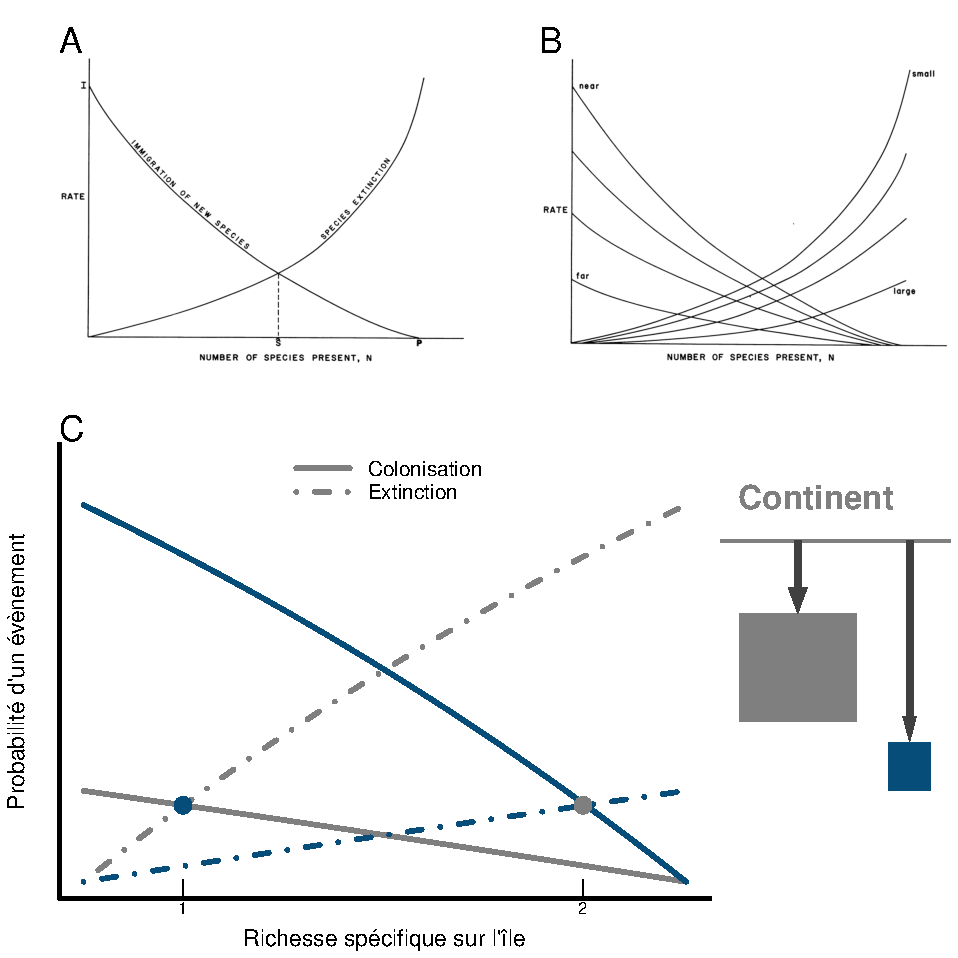
\includegraphics{fig/fig1.pdf}
\caption{\textbf{La Théorie de la biogéographie des Iles.} L'évolution
des taux de colonisation et d'extinction est présentée pour deux îles
aux caractéristiques différentes. Les tailles relatives des îles et les
distances qui les séparent du continent sont schématisées à droite du
graphique, les couleurs associent les îles à leurs courbes respectives.
Le pool d'espèce régional (\(P\)) est constitué de 100 espèces, les taux
de colonisation et d'extinction sont exprimés en terme de probabilité
d'évènement. Les points où colonisation et extinction s'équilibrent sont
marqué par les symboles en gris.\label{fig:figMW}}
\end{figure}

\subsection*{L'empreinte historique de la Théorie de la Biogéographie
des Iles de MacArthur et
Wilson}\label{lempreinte-historique-de-la-thuxe9orie-de-la-bioguxe9ographie-des-iles-de-macarthur-et-wilson}
\addcontentsline{toc}{subsection}{L'empreinte historique de la Théorie
de la Biogéographie des Iles de MacArthur et Wilson}

Dans leur livre \emph{The Theory of Island Biogeography}, MacArthur et
Wilson indique dans leur préface qu'il ne pensait pas que leur
résisterait longtemps surtout quand elle serait testé empiriquement :

\begin{quote}
We do not seriously believe that that the particular formulations
advanced in in the chapters to follow will fit for very long the
exacting results of future empirical invesitgation. (péface de l'édition
de 1967)
\end{quote}

Et pourtant fort près de 50 ans après la parution de leur ouvrage, la
vision distilé est toujours aussi vive en témoigne le livre paru en 2010
\emph{The Theory of Island Biogeography Revisited} (Losos and Ricklefs,
2010) et la reve par Warren et collègue (Warren et al., 2015) qui montre
bien que les île ont servie de moèdeles et que la vision est un point
les travaux sont capitale.

Le terme des îles est centraled mais il s'agit bien d'une théorie de la
biogéogroahie. reflète aussi l'importance des îles dans l'édification
d'une théorie isolation lux de migraotion simple / assemblage moins
nombreux / conséquence d'une manipultion limité à l'île / 5\% mais
répétable ? / un oacth isolé et peut être que flux au île (Simberloff,
1974) Pourquoi les îles en fait isolé flux et gros contraste mailand -
island alors qu'elles sontproches.. Les îles qui occupent le coeur de
l'ouvrage de Wallace et de MAcArthur et Wilson ont été essentiel poour
comprendre les processus qui forme la sitributn des espèces. Elle sosn
tproches du continent et peuvent être si différenetes la nature eotique
des piles à forcer les auteurs à comprendre l'origine de leur
singularit.é et ces sur ces bout de terre isolé qu'ils ont trouv.s des
réposnes historques ais ausso spataile qui a parmis d'aller vers des
dévelppemnt encore aujourd'hui très actis. La quête de cees honmes et de
bien d'autres reste finalemnt de comprendre pourquoi les espèces sont ou
elles sont et de comproendre ce qui les amanerner la. Meilleur
explication pour des arrangemnets spatiaux singuliers sont des processus
temporels. Faire émerger des règles mon apport amener des interactions.

Preston 1962 a lié species abundance et =\textgreater{} impact enorme
sur la conservation et encore aujourd'hui bien que simplifié les calculs
permettent de comprendredsimplementr dans quelles directions nous allons
{[}article NewYork Times{]} Malgré la 50 ans de depuis la publication du
Livre et premier articles a lasuorise de auiteure eux meme
=\textgreater{} publications récentes qui repartent de la théorie des
îles ; l'ecolet Warren et gravel and all

Dans la réédition de 2001 {[}{]} Wilson rappelle que le problème :

\begin{quote}
``The flaws of the book lie in its oversimplification and
incompleteness, which are endemic to most efforts at theory and
synthesis.''
\end{quote}

Diminuer la composante historqiue à la recherche de loi et j'ajouterais
aussi simple soit elle raffiner par la suite

\subsubsection{La théorie des
métapopulations}\label{la-thuxe9orie-des-muxe9tapopulations}

=\textgreater{} chapitre de Hanski

\subsubsection{La théorie neutre de l'écologie et le débat qu'elle
soulève}\label{la-thuxe9orie-neutre-de-luxe9cologie-et-le-duxe9bat-quelle-souluxe8ve}

Ecological equivalence des individus OK mais peut-être que l'abondance
des interactions expliques aussi

=\textgreater{} chapitre dans revisited

Problème si explication alternatives possibles alors on n'est pas obligé
de mettre pour expliquer quoi que ce soit. De plus savons nous si c'est
discernable ??? Si le deux relation aire espèce sont différentes d'un
groupe à l'autre alors oui\ldots{} Mais sinon\ldots{} Non.

Oppositon à la niche.

(Chapitre 8 TIB first paragraph)

Le concept récent de biodiversité. However ecological equivalence in
``the niche is a mapping of population dynamics onto this space''
({\textbf{???}}) vers le fonctionnemt des ecosystèmes levier d'action
vers une approche plus utilitariste mais qui donne uns certaine
proximité avec les eécosytèmes Loreau et al. (2001)

\subsection{Aller plus loin, Enjeux
théoriques}\label{aller-plus-loin-enjeux-thuxe9oriques}

L'effort théorique nécessaire en biogéographie porte sur l'intégration
ordonnée de concepts clés issus de différents champs de l'écologie
\cite{Thuiller2013}. Ainsi, alors que les conditions climatiques et plus
généralement la géographie physique sont classiquement évoquées pour
expliquer la répartition des espèces \cite{Kearney2004}, les
interactions entre espèces sont quant à elles souvent occultées. De
même, bien que les processus évolutifs soient souvent évoqués comme
déterminants majeurs de la diversité des espèces \cite{Rosindell2011},
leurs effets à court terme sont souvent ignorés \cite{Parmesan2006} dans
les scénarios décrivant la biodiversité de demain \cite{Lavergne2010}.
La difficulté principale est alors de produire des modèles (théoriques
en première instance) qui intègrent l'ensemble des processus et les
relations qu'ils entretient \cite{Thuiller2013} tout en gardant une
relative simplicité. Une théorie intégrative en biogéographie pourrait
être le meilleur point d'ancrage pour construire de nouvelles approches
appliquées. Avec une telle théorie en main, nous pourrions aller vers
l'enjeux majeurs de ces dernières années en biogéographie : relâcher les
hypothèses que les modèles classiques de répartitions des espèces
d'aujourd'hui utilisent (notamment en occultant les interactions) pour
prédire la biodiversité de demain \cite{Guisan2011}.

Dans le projet ici présenté, nous proposons de construire des modèles
théoriques plus intégratifs en repartant d'un modèle théorique
classique, celui de la théorie de la biogéographie des îles proposée par
MacArthur et Wilson \cite{MacArthur1967}. Dans un premier temps, nous y
ajoutons les interactions entre espèces et une relation explicite avec
l'environnement abiotique au travers d'une approche communauté centrée
qui étend le modèle classique. Dans un second temps, nous combinons une
approche population centrée et les processus évolutifs pour une
biogéographie insulaire plus mécaniste. Enfin, au regard des enjeux que
soulève le rôle des interactions entre espèces dans la construction de
la biodiversité, nous réfléchissons sur l'inférence d'espèces
interdépendantes.

différentes théories pour différentes échelles ??

De part son pouvoir explicatif et son élégance, le modèle de MacArthur
et Wilson est un point de départ approprié pour construire des modèles
plus intégratifs en intégrant explicitement des processus écologiques et
évolutifs. Cette idée n'est pas nouvelle et les auteurs de la TIB ont
étudié un certain nombre de processus écologiques. Notamment, ils ont
intégré les phénomènes de spéciation \cite{MacArthur1967} et réfléchis
sur l'importance des interactions quant à la répartition des espèces
\cite{MacArthur1984}. Néanmoins, dans le modèle classique, l'ensemble de
ces aspects sont absents, l'idée que les processus écologiques importent
peu aux larges échelles domine. Nous allons, dans ce projet, à
l'encontre de cette idée et proposons de construire des modèles
intégratifs qui étendent la TIB.

isolation / faune particulière des îles

\section*{Le rôle des interactions dans la distributiondes
espèces}\label{le-ruxf4le-des-interactions-dans-la-distributiondes-espuxe8ces}
\addcontentsline{toc}{section}{Le rôle des interactions dans la
distributiondes espèces}

L'objet central de ma thèse est l'introduction de ma thèse est d'essayer
de regrader la théorie de la biogéographie et notamment quelles
onfornatiosn 'écologie des réseayx peurt ameenr de la lumière sur la
théorie. Dans cette dernière partie de mon introduction, je présente
avec pkus de délément l'importance de l'intriduction des onteractions
dans une théorie de la biogéographi. Cela me permettra d'introduire nes
contributions qui seront détaillées dans ma thèse.

\begin{quote}
However, it is argued that applying bio-climatic models at macro-scales,
where climatic influences on species distributions are shown to be
dominant, can minimize the impact of biotic interactions. Indeed, the
fact that a number of bioclimatic models have been highly successful at
simulating current species distributions at certain scales is in
fundamental disagreement with the proposition that species distributions
cannot be adequately defined by climatic factors alone. (Pearson and
Dawson, 2003)
\end{quote}

\begin{quote}
We will never be able to predict the future with accuracy, but we need a
strategy for using existing knowledge and bioclimatic modeling to
improve understanding of the likely effects of future climate on
biodiversity. (Araujo and Rahbek, 2006).
\end{quote}

\subsection{Interaction et
biogeographie}\label{interaction-et-biogeographie}

Accent sur les cascading effect est surtout un problème de l'instabiilté
({\textbf{???}}) Il ya aussi l'article perturbant de Säterberg et al.
(2013) qui montre que le fait qu'une espèce soit (ex. pêche) peut
conduirte à des extinctions d'autres espèces lié dans le réseau\ldots{}
Ces deux exemple montrent que les interactions peuvent mener à des
problèmes de prédicitons et donc porblèmes sur prévoir les services
ecosystémiques et c'est appuyer par Cahill et al. (2013) qui nous
indique en somme que le changemnr des interactiosn bioiqtess ets la voie
privilégié d'extintionciton dans un contexte de chanegnmtn climatique

On nous fait miroiter que finalement que l'érosion de la biodiversité
est dramatiques et le ressort actuel pour faire un levier face à cela
c'est les services ecosystémiques qui sont actuelelemet l'argument choc
pour renforcer la production de la nature. Il y a un côté pervers qui
est la financiarisation et la substituabilité l'argent oeut alors être
utilisée pour intervertir ou alors remplacer un type d'écisystème par un
autre ailleurs\ldots{} En fait on a l'impressonq ue c'est pus un
principe de précaution qui erst invoquer et ultimement il est
vraisemblable que la destruction de la nature tel que nous la
connaissons soit dans le future un générateur de conflit\ldots{}. et
uttiment on a a craindre de faire un panete invivable pour nous mêm.

Mais les changement sont des remplacemnt et pour la conservation on peut
se demander les startégie. Dans son arctile `Don't juge a species on
their origin' Mark Davis prend à revers un sertain nombre d'idée recu et
souligne qye les effects des invedeurs peuvent être positives Davis et
al. (2011).

Les ramges comme un fait (wallace chap 2) des espèces avec des larges
avec des grandes ranges Loddigésie admirable (\emph{Loddigesia
mirabilis}) seul collibris de son genre vs Lièvre variable (\emph{Lepus
timidus}) nomnbre d'espèce dans un genre vaire beaucoup =\textgreater{}
un autre indice de solution pas fructifiées\ldots{} Pithacia Monathus vs
Pithecia pythecia separé par une rivière Geographical Ecology
=\textgreater{} patterns in the distribution of spceies 2 espèces
proches des ranges très séparéed =\textgreater{} species Bonobo et
cChimpanzés

L'évolution = le hasard et la nécessité est un moteur de la répartiton
mais aussi la composante historiqe de la biologie. Cette dimension
fascinante implique aussi nous focalisé sur des explications singulière
souvent pas évident qui permettent de conformer le type de facteurs
impliqué dans la variation des ranges mais nous amène pas encore à
trouver des règles précices.

Wallace conclut :28 qu'une théorie générale doit tenir compte des
variation range et proximité des espèces porches et des overlapp.

\begin{quote}
Both competition and predation appear now to be much more important in
biogeography than peopl had formely guesses
\end{quote}

chap 2 geographical ecology

il prend comme exemple la compétition entre oiseau et un manque de
ressource pour une année partiuculièremnet sévère et que 19 and pas
assez pour voir et il conclut que

\begin{quote}
This is the main reason most evidence for competition is from
biogepgraphers.
\end{quote}

Distributiin des fauvettes \emph{Crateroscelis robusta} et \emph{C.runa}

Mais le porblème étant que le signal n'est visible que si on a des
données sur 20and.

Le problème

Parallèle entre information des traits sur le régime allimentaire et
l'information dans les ranegs est-ce cela qui conduit les ecologistes à
être des statisticuencs. et l'info dans l'ADN

la question a été pourquoi il y a autant d'espèces mais je pense qu'un
equestion légèremnetn différentes n'a pas été assez invextie : pourquoi
peuvent-elles être si nombreuse\ldots{}. La limite est toujours OK si
assez pour 2 ou plus.

\subsection{Interactions écologique et
TIB}\label{interactions-uxe9cologique-et-tib}

\begin{quote}
(:154) ``Does the environment dictate the structure of the community, or
are the species a fairly random assemblage?
\end{quote}

\begin{quote}
A few decades ago it as fashionable for ecologist to study communities
in the arctic on the grounds that these would be very simple communities
and hence easy to understand. Many excellent ecologists still follow
this belied, but there are others who feel that it may be easier to
understand the extremely complex communities. This sounds paradoxical:
How can a more complex communities by easier to understand? A possible
answer might be that complex community has has strong interactions among
species so that the lives of the separate species are less independent
than in a simple community. Where there is greater interdependence,
patterns may be more conspicuous."
\end{quote}

\subsection{Oubli de ce facteur important
de}\label{oubli-de-ce-facteur-important-de}

Ls SMDS\ldots{}

Les interactions intra et inter spécifiques constituent un facteur
rapidement pressenti comme responsable de la distribution spatiale des
espèces \cite{Levin1974}. L'interdépendance des espèces conditionne, en
effet, l'aspect favorable de l'environnement au sens large (biotique et
abiotique). Ainsi Godsoe \textit{et al.} 2012, mettent en équations le
caractère favorable de l'environnement pour une espèce donnée en terme
de probabilité de présence d'une autre espèce et de la nature de leur
interaction \cite{Godsoe2012}. De même, Holt et Barfield 2009 montrent
l'impact de la prédation sur la répartition d'espèces en compétition
\cite{Holt2009} insistant ainsi sur le rôle majeur des interactions.
Davis \textit{et al.} 1998 ont montrés que, pour trois drosophiles en
compétition, l'effet d'un parasitoïde n'est pas le même le long d'un
gradient selon que les espèces sont seules ou ensemble \cite{Davis1998}.
Récemment, des efforts ont été réalisés pour mettre en évidence
l'importance de l'interdépendance des espèces dans les données aux
larges échelles spatiales \cite{Gotelli2010}. On trouve actuellement
dans la littérature une grande motivation pour les intégrer dans les
modèles de distribution d'espèces \cite{Kissling2011, Guisan2011}. Des
efforts théoriques sont encore nécessaires pour arriver à de telles
approches. Néanmoins, rapprocher différents champs de l'écologie peut
s'avérer d'une utilité majeure. Jabot et Bascompte \cite{Jabot2012}
2012, ont d'ailleurs montré l'importance des interactions pour
comprendre la distribution des espèces en rapprochant écologie des
réseaux et un modèle de metacommunauté. De même Gravel \textit{et al.}
2011 \cite{Gravel2011b} introduise l'interdépendance proie-prédateur
dans le modèle classique de MacArthur et Wilson menant aux prémices
d'une théorie trophique de la biogéographie des îles.

L'ajout des interactions dans un modèle incluant l'environnement
abiotique interroge la relation que les deux processus entretiennent. Si
les espèces n'ont pas les mêmes performances dans différents milieux du
fait de leur physiologie, pour les mêmes espèces considérées, les
réseaux n'ont pas de raison d'être identiques d'un milieu à un autre.
C'est sur ce fait que Poisot \textit{et al.} 2012 ont proposé une mesure
de dissimilarité des réseaux \cite{Poisot2012}. Defossez \textit{et al.}
montrent que les interactions négatives entre l'hêtre commun
(\textit{Fagus Sylvaitca}) et les micro-organismes du sol diminuent avec
l'altitude \cite{Defossez2011}. Ainsi, les contraintes biotiques sont à
relier à l'environnement \cite{Brooker2006,Canham2006} et un modèle
intégratif doit donner un cadre cohérent à ces rétroactions entre
processus. Enfin, l'importance des interactions est à mettre en relation
avec l'échelle considérée \cite{Peterson2011}. Pour deux espèces en
interaction, plus l'échelle d'étude est large, moins les effets des
interactions locales sont susceptibles d'être capturés, le pouvoir
explicatif de la présence d'une espèce sur l'autre peut être alors
discutable \cite{Araujo2007}. Comprendre quels sont les processus à
prendre en compte aux différentes échelles spatio-temporelles et
comprendre comment le changement d'échelle affecte nous prédictions est
aussi un véritable challenge en biogéographie \cite{Martinez2012}.

\section*{Intégrations des contraintes biotiques et de la théorie à la
recherche de signaux de
d'intéraction}\label{intuxe9grations-des-contraintes-biotiques-et-de-la-thuxe9orie-uxe0-la-recherche-de-signaux-de-dintuxe9raction}
\addcontentsline{toc}{section}{Intégrations des contraintes biotiques et
de la théorie à la recherche de signaux de d'intéraction}

Dans ma thèse j'ai oassé du temps à essayer de mettre au point un modèke
qui donnait de la substace aux idées de MacArthur et Wilson een etandant
le travai initié par Gravel et collègues pour aller plus loin dans la
compréhension des effets joints des interactions et des contraintes
abiotiques. C'est aussi ce qui m'a animé pour en mettre en place la
compréhesin dans les données de co-occurrence avant d'aller m'y
confronter frongalemnet. Ma dernière intergtaion a Été de trouver des
pistes pour allerr plus loin dans la théorie et explorer des pistes que
je n'avais pas encore dxplorer mais qui seront à court terme les
directions que je souhaite explorer.

\subsection*{Étendre la théorie de MacArthur et
Wilson}\label{uxe9tendre-la-thuxe9orie-de-macarthur-et-wilson}
\addcontentsline{toc}{subsection}{Étendre la théorie de MacArthur et
Wilson}

\subsection*{Comprendre les conséquence en terme de
co-occurrece}\label{comprendre-les-consuxe9quence-en-terme-de-co-occurrece}
\addcontentsline{toc}{subsection}{Comprendre les conséquence en terme de
co-occurrece}

\subsubsection*{Abondance des données}\label{abondance-des-donnuxe9es}
\addcontentsline{toc}{subsubsection}{Abondance des données}

Les atouts actuels de la biogéographie sont 1- une quantité importante
d'information relative aux présences d'espèces et au climat et 2- des
modèles corrélatifs puissants qui décrivent précisément le lien entre
l'espèce et son environnement abiotique. Le terme abiotique peut prêter
à confusion dans la mesure où les espèces elles-mêmes peuvent modifier
des variables dîtes abiotiques. Par exemple, les végétaux peuvent avoir
un grand impact sur les variables abiotiques locales comme la
température et l'humidité du sol \cite{Breshears1998}. Certains auteurs
font une distinction précise en utilisant les termes de
\textit{scenopoetiques} pour les variables environnementales sur
lesquels les espèces ne peuvent influer et de
\textit{dynamiquement liées} pour les autres \cite{Peterson2011}. Nous
occulterons volontairement ces-dernières, l'environnement abiotique dont
il est ici question n'est donc pas dynamiquement lié aux espèces.

\subsubsection*{Potential interactions}\label{potential-interactions}
\addcontentsline{toc}{subsubsection}{Potential interactions}

Vespa aussi au Amérqieu la densit. des traffic\ldots{}

Multi couche de distrobution dans le cas du frelon asiatique Villemant
et al. ({\textbf{???}}) ont montrés que superposition du genre
\emph{Vespa} et notamment au niveau asiatique énormément aisin
l'inférence se fait sur des données qui comporte une empreinte de
condition et localemnt éteinte alors que possiblement comtraite qui ne
seront pas en France\ldots{}

Décrire l'organisation spatiale des êtres vivants et en comprendre les
mécanismes sous-jacents, tels sont les objectifs ambitieux de la
biogéographie \cite{MacArthur1967}. Cette discipline a récemment
percolée au sein de la société civile via le concept de biodiversité. Le
regard des citoyens se posent attentivement sur le devenir de la
biodiversité dans le contexte actuel des changements globaux. La
biogéographie, par son essence, peut apporter des réponses à ce
questionnement ambiant \cite{Whittaker2005}. Cependant, pour y parvenir,
des défis techniques et théoriques majeurs restent à surmonter
\cite{Beck2012}.

\subsection*{Chercher des signaux de
co-occurrence}\label{chercher-des-signaux-de-co-occurrence}
\addcontentsline{toc}{subsection}{Chercher des signaux de co-occurrence}

gecko australien généraliste \emph{Heteronotia binoei}
=\textgreater{}~alors peut être que ça marche bien mais sur une espèce
spécialiste ??

\subsection*{Information dans les
distributions}\label{information-dans-les-distributions}
\addcontentsline{toc}{subsection}{Information dans les distributions}

\section*{Dépasser les questionnemnet sur les
espèces}\label{duxe9passer-les-questionnemnet-sur-les-espuxe8ces}
\addcontentsline{toc}{section}{Dépasser les questionnemnet sur les
espèces}

\section*{Aller de l'avant}\label{aller-de-lavant}
\addcontentsline{toc}{section}{Aller de l'avant}

\subsection{DEB}\label{deb}

\subsection{Espoir sur la}\label{espoir-sur-la}

Le travail de Gotelli \textit{et al.} est également un exemple de
démarche intégrative où un nombre important de processus peuvent être
inclus via un système de combinaison de scénarios et tester par
simulations stochastiques \cite{Gotelli2009}. Enfin, en construisant des
réseaux basés sur la cooccurrence des espèces, Araújo \textit{et al.}
revisitent le problème de l'interdépendance des espèces
\cite{Araujo2011} : ils s'interrogent sur la résistance des réseaux de
cooccurrence obtenus face aux futurs changement climatiques, ils mettent
ainsi en évidence des risques accrus de perte des espèces les moins
connectés (celles qui cooccurent moins). Ces travaux témoignent de la
volonté d'une biogéographie intégrative.

C'est impressionnant de voir comment un auteur en repartant de simple
considération telle que la taile le volume peut arriver à construire une
théorie à la fois simple, fondée et predictive. mettant de la cohérence
dansune accumulation de fait.

=\textgreater{} problème SDMS quand inférencefait sur les données
d'espèces la force c'est d'avoir des mesures ++ et indépendante quelquee
part c'est vrai mais la source d'inforation est très brouillé et on peut
se demander se que l'on peut obtenir comme infornation\ldots{}.

\subsection*{Traits fonctionnels}\label{traits-fonctionnels}
\addcontentsline{toc}{subsection}{Traits fonctionnels}

Les traits fonctionnels sont des propriétés mesurables sur les
organismes en relation avec leurs performances et leur rôle dans
l'écosystème \cite{McGill2006}. Les traits étudiés peuvent être de
différentes natures, 1-morphologiques : taille de différentes parties du
corps, position des yeux, taille des oeufs chez les organismes ovipares,
taille des graines pour les végétaux, 2- physiologiques : taux
métaboliques de bases, stœchiométrie (rapport de la concentration entre
divers éléments qui compose l'organismes)
\cite{McGill2006,Albouy2011,Litchman2008}. Un ensemble approprié de ces
propriétés peut être un outil puissant pour décrire un ensemble d'espèce
dans un même espace. Leur proximité dans l'espace des traits est alors
un indice précieux d'une proximité fonctionnelle. Ainsi, à l'aide de 13
traits ecomorphlogiques, Albouy \textit{et al.} 2011 parviennent à
prédire les guildes trophiques de 35 espèces de poissons de la
Méditerranée \cite{Albouy2011}. Edwards \textit{et al.} 2013 montrent
que l'effet saisonnier sur une communauté de phytoplancton dans la
Manche peut être capturé à l'aide de traits décrivant : le taux maximal
de croissance, la compétitivité pour la lumière et l'azote
\cite{Edwards2013}. La distribution des traits fonctionnels au sein de
la biodiversité est aussi une entrée de choix pour réfléchir quand à la
fragilité potentielle des fonctions remplies par les écosystèmes
\cite{Mouillot2013}. \%DG: je comprends cette citation de Mouillot, mais
juste une mise en garde contre ce type de référence. Mouillot se base
sur l'hypothèse que les traits nous informent du fonctionnement, sans
jamais documenter cette relation. Ce qui est souvent le cas, et par
conséquent contribue à bâtir des mythes dans la littérature qui à
l'occasion ne sont pas toujours bien appuyés. L'approche par traits est
un bel exemple, on a édifié rapidement une structure conceptuelle sur
les traits, mais on n'a pas solidement appuyé le concept sur de bonnes
bases empiriques.

L'approche de la biodiversité par les traits fonctionnels est plus
quantitative que l'approche taxonomique et permet de déduire un grand
nombre de propriétés en se passant de la connaissance de leur identité.
Ainsi McGill, dans son article d'opinion de 2006, propose une approche
nouvelle de l'écologie des communautés qui transforme les questions
centrées autour des espèces par des questions qui interrogent la
répartition et la variabilité des traits \cite{McGill2006}. L'emploi des
traits fonctionnels est en fait un appel à une écologie plus mécaniste,
qui se penche sur la physiologie des organismes, en prend les faits les
plus importants (relativement au problème traité) pour les placer dans
un espace de traits commun. Cette approche est aussi en lien avec la
controversée théorie métabolique en écologie
\cite{Brown2004, Price2012}. Dans cette théorie un certain nombre de
grandeurs (comme le taux métabolique) sont reliées à la biomasse
corporelles de l'adulte, fournissant ainsi en un seul trait de
nombreuses relations pour des groupes d'organismes très différents. Par
ces nouvelles approches, l'espérance de s'extraire de la seule identité
des espèces est accrue, l'idée d'avoir des règles générales se
concrétise.

Dans une théorie intégrative de la biogéographie, les traits
fonctionnels peuvent être un pivot très intéressant pour rassembler les
différents concepts que nous avons développés dans les paragraphes
précédents. Les traits peuvent tout d'abord être mis en relation avec le
milieu abiotique. Le taux métabolique ou encore la sensibilité à la
sécheresse sont des indices performant pour décrire la survie dans un
milieu donné \cite{Kearney2004,Engelbrecht2007} que l'on peut capturer
sous forme de traits. Kearney \textit{et al.} 2010 propose une approche
prometteuse dans laquelle, l'environnement physique, la disponibilité
des ressources et la dynamique énergétique sont reliées par les traits
fonctionnelles le tout aboutissant à un modèle de distribution très
mécanistes. La structure d'un réseaux peut également être dérivée à
partir de l'espace des traits. Dans leur méthode proposée cette année,
Gravel \textit{et al.} infèrent les paramètres du modèle de niche de
Williams et Martinez \cite{Williams2000} à partir des relations de masse
du corps entre proie et prédateurs \cite{Gravel2013}. Ils sont alors en
mesure de dériver un réseau global pour un ensemble d'espèce donné.
Enfin, en tant qu'expression phénotypique, les traits fonctionnels sont
soumis aux processus évolutifs. Sur les temps longs, l'expression de
l'évolution résulte en la modification progressive des traits qui se
répercute sur l'ensemble des propriétés qui en découle. Ainsi la
considération d'une modification des traits est une approche simple et
réaliste pour introduire les processus évolutifs et leurs conséquences
\cite{Guill2008,Loeuille2005}.

La niche c'est quoi on en a deux definition ultr classique mais elles
sont très porblématiques. Il y a des tentatives de synthèse mais le
problèmes est toujours là.

Partir du development de la niche et des hypotheses clef comme
l'heterogeneité spatiale qui peut accroitre la biodiversité un exemple
c'est les ecoulemnents à petites faible echelles de l'hydrologie niche
hdrologique à fable échelles Letten et al. (2015) repartition
hydrologique les hypothèses sont que qui explique celon les différentes
besoin des espèces (principes de la niche) que besoin différemtes me
répartition des espèces. Cette idées est

A large espes répartition de la biodiversité on quantifie la différence
depuis les mesures classiques Simpson, alpha gamma beta qui sont
étendues au réseau Poisot et al. (2012). Mais quand on chnage d'echelle
on arrive rarement à quelques choses de concluant pour l'integration des
interactions. Pourtant il ya des exemples convaicant comme celui de
Gitelli.

Les interactions c'est quoi ce qu'on en fait. Les interactions quelles
pourrait être leur conséquence à large échelle ?

Mais au-dela de cela il yt a un besoin de règles. L,écoligies cherche
ces règles et essayes de faire le max sans trip de succès. Les traits
sont un gran despoir. On a besoinde rule on reste descriptive il y a des
relation EH-Bioversité, SAR, Diversité-équilibre diversité
fonctionnenemnt qui sont partielelemnt reliées et des théries débat
theories neutre theéor de la niche Stein et al. (2014). Dans cette
review Stein et al. (2014) montre que vegettaion est inportnates ce qui
eimplique des inbteractions. Théorie allométrique prometteuse en ce sens
qu'elle loi physiques. Différents concept autrour d'une même notion sur
plusieurs paradigme pour une même notion sur les metacommunity Leibold
et al. (2004) il peuvent co-exister mais faudrait les savoir ce qui fait
qu'on a pus l'un ou l'autr.

La puissance de la Biogéographie est aussi sont implications dans des
cas très concrets Cirtwill and Stouffer (2015) mais aussi ne puissance
exploratoire théoriques Gravel et al. (2011) Cazelles et al. (2015) des
îles l'idée des interactions à déjà montré ça pertinence sur plusieurs
exemples. Cirtwill and Stouffer (2015)

La bonne unité d'analyse ? D'où parti r?

\begin{quote}
Generalist consumers should typically be weakly coupled to any one of
their prey populations because, when feeding on many different species,
they cannot be strongly coupled to any one of them Murdoch et al. (2002)
\end{quote}

\hypertarget{refs}{}
\hypertarget{ref-Allesina2012a}{}
Allesina, S., Tang, S., 2012. Stability criteria for complex ecosystems.
Nature 483, 205--208.
doi:\href{https://doi.org/10.1038/nature10832}{10.1038/nature10832}

\hypertarget{ref-Araujo2006}{}
Araujo, M.B., Rahbek, C., 2006. How Does Climate Change Affect
Biodiversity? Science 313, 1396--1397.
doi:\href{https://doi.org/10.1126/science.1131758}{10.1126/science.1131758}

\hypertarget{ref-Beck2012}{}
Beck, J., Ballesteros-Mejia, L., Buchmann, C.M., Dengler, J., Fritz,
S.A., Gruber, B., Hof, C., Jansen, F., Knapp, S., Kreft, H., Schneider,
A.-K., Winter, M., Dormann, C.F., 2012. What's on the horizon for
macroecology? Ecography 35, 001--011.
doi:\href{https://doi.org/10.1111/j.1600-0587.2012.07364.x}{10.1111/j.1600-0587.2012.07364.x}

\hypertarget{ref-Beck2014a}{}
Beck, J., Böller, M., Erhardt, A., Schwanghart, W., 2014. Spatial bias
in the GBIF database and its effect on modeling species' geographic
distributions. Ecological Informatics 19, 10--15.
doi:\href{https://doi.org/10.1016/j.ecoinf.2013.11.002}{10.1016/j.ecoinf.2013.11.002}

\hypertarget{ref-Bellard2012}{}
Bellard, C., Bertelsmeier, C., Leadley, P., Thuiller, W., Courchamp, F.,
2012. Impacts of climate change on the future of biodiversity. Ecology
letters 15, 365--377.
doi:\href{https://doi.org/10.1111/j.1461-0248.2011.01736.x}{10.1111/j.1461-0248.2011.01736.x}

\hypertarget{ref-Cahill2013}{}
Cahill, A.E., Aiello-Lammens, M.E., Fisher-Reid, M.C., Hua, X.,
Karanewsky, C.J., Ryu, H.Y., Sbeglia, G.C., Spagnolo, F., Waldron, J.B.,
Warsi, O., Wiens, J.J., 2013. How does climate change cause extinction?
Proceedings. Biological sciences / The Royal Society 280, 20121890.
doi:\href{https://doi.org/10.1098/rspb.2012.1890}{10.1098/rspb.2012.1890}

\hypertarget{ref-Cazelles2015b}{}
Cazelles, K., Mouquet, N., Mouillot, D., Gravel, D., 2015. On the
integration of biotic interaction and environmental constraints at the
biogeographical scale. Ecography n/a--n/a.
doi:\href{https://doi.org/10.1111/ecog.01714}{10.1111/ecog.01714}

\hypertarget{ref-Cirtwill2015}{}
Cirtwill, A.R., Stouffer, D.B., 2015. Knowledge of predator-prey
interactions improves predictions of immigration and extinction in
island biogeography. Global Ecology and Biogeography n/a--n/a.
doi:\href{https://doi.org/10.1111/geb.12332}{10.1111/geb.12332}

\hypertarget{ref-Connor1979}{}
Connor, E.F., Simberloff, D., 1979. The Assembly of Species Communities:
Chance or Competition? Ecology 60, 1132.
doi:\href{https://doi.org/10.2307/1936961}{10.2307/1936961}

\hypertarget{ref-Davis2011}{}
Davis, M. a, Chew, M.K., Hobbs, R.J., Lugo, A.E., Ewel, J.J., Vermeij,
G.J., Brown, J.H., Rosenzweig, M.L., Gardener, M.R., Carroll, S.P.,
Thompson, K., Pickett, S.T. a, Stromberg, J.C., Del Tredici, P., Suding,
K.N., Ehrenfeld, J.G., Grime, J.P., Mascaro, J., Briggs, J.C., 2011.
Don't judge species on their origins. Nature 474, 153--4.
doi:\href{https://doi.org/10.1038/474153a}{10.1038/474153a}

\hypertarget{ref-Diamond1975}{}
Diamond, J.M., 1975. Assembly of species communities, in: Cody, M.L.,
Diamond, J.M. (Eds.), Ecology and Evolution of Communities. Harvard
University Press, Cambridge, Massachusetts, USA., pp. 342--444.

\hypertarget{ref-Elith2006}{}
Elith, J., H. Graham, C., P. Anderson, R., Dudík, M., Ferrier, S.,
Guisan, A., J. Hijmans, R., Huettmann, F., R. Leathwick, J., Lehmann,
A., Li, J., G. Lohmann, L., A. Loiselle, B., Manion, G., Moritz, C.,
Nakamura, M., Nakazawa, Y., McC. M. Overton, J., Townsend Peterson, A.,
J. Phillips, S., Richardson, K., Scachetti-Pereira, R., E. Schapire, R.,
Soberón, J., Williams, S., S. Wisz, M., E. Zimmermann, N., 2006. Novel
methods improve prediction of species' distributions from occurrence
data. Ecography 29, 129--151.
doi:\href{https://doi.org/10.1111/j.2006.0906-7590.04596.x}{10.1111/j.2006.0906-7590.04596.x}

\hypertarget{ref-Elith2009a}{}
Elith, J., Leathwick, J.R., 2009. Species Distribution Models:
Ecological Explanation and Prediction Across Space and Time. Annual
Review of Ecology, Evolution, and Systematics 40, 677--697.
doi:\href{https://doi.org/10.1146/annurev.ecolsys.110308.120159}{10.1146/annurev.ecolsys.110308.120159}

\hypertarget{ref-Engelbrecht2007}{}
Engelbrecht, B.M.J., Comita, L.S., Condit, R., Kursar, T. a, Tyree,
M.T., Turner, B.L., Hubbell, S.P., 2007. Drought sensitivity shapes
species distribution patterns in tropical forests. Nature 447, 80--82.
doi:\href{https://doi.org/10.1038/nature05747}{10.1038/nature05747}

\hypertarget{ref-Gravel2011c}{}
Gravel, D., Bell, T., Barbera, C., Bouvier, T., Pommier, T., Venail, P.,
Mouquet, N., 2011. Experimental niche evolution alters the strength of
the diversity--productivity relationship. Nature 469, 89--92.
doi:\href{https://doi.org/10.1038/nature09592}{10.1038/nature09592}

\hypertarget{ref-Hannah2013}{}
Hannah, L., Roehrdanz, P.R., Ikegami, M., Shepard, A.V., Shaw, M.R.,
Tabor, G., Zhi, L., Marquet, P.a., Hijmans, R.J., 2013. Climate change,
wine, and conservation. Proceedings of the National Academy of Sciences
110, 6907--6912.
doi:\href{https://doi.org/10.1073/pnas.1210127110}{10.1073/pnas.1210127110}

\hypertarget{ref-Hijmans2005}{}
Hijmans, R.J., Cameron, S.E., Parra, J.L., Jones, P.G., Jarvis, A.,
2005. Very high resolution interpolated climate surfaces for global land
areas. International Journal of Climatology 25, 1965--1978.
doi:\href{https://doi.org/10.1002/joc.1276}{10.1002/joc.1276}

\hypertarget{ref-Hortal2011}{}
Hortal, J., Diniz-Filho, J.A.F., Bini, L.M., Rodríguez, M.Á., Baselga,
A., Nogués-Bravo, D., Rangel, T.F., Hawkins, B.A., Lobo, J.M., 2011. Ice
age climate, evolutionary constraints and diversity patterns of European
dung beetles. Ecology Letters 14, 741--748.
doi:\href{https://doi.org/10.1111/j.1461-0248.2011.01634.x}{10.1111/j.1461-0248.2011.01634.x}

\hypertarget{ref-Kearney2004}{}
Kearney, M., Porter, W.P., 2004. MAPPING THE FUNDAMENTAL NICHE:
PHYSIOLOGY, CLIMATE, AND THE DISTRIBUTION OF A NOCTURNAL LIZARD. Ecology
85, 3119--3131.
doi:\href{https://doi.org/10.1890/03-0820}{10.1890/03-0820}

\hypertarget{ref-Kefi2015}{}
Kéfi, S., Berlow, E.L., Wieters, E.A., Joppa, L.N., Wood, S.A., Brose,
U., Navarrete, S.A., 2015. Network structure beyond food webs: mapping
non-trophic and trophic interactions on Chilean rocky shores. Ecology
96, 291--303.
doi:\href{https://doi.org/10.1890/13-1424.1}{10.1890/13-1424.1}

\hypertarget{ref-Kefi2012}{}
Kéfi, S., Berlow, E.L., Wieters, E.A., Navarrete, S.A., Petchey, O.L.,
Wood, S.A., Boit, A., Joppa, L.N., Lafferty, K.D., Williams, R.J.,
Martinez, N.D., Menge, B.A., Blanchette, C.A., Iles, A.C., Brose, U.,
2012. More than a meal\ldots{} integrating non-feeding interactions into
food webs. Ecology Letters 15, 291--300.
doi:\href{https://doi.org/10.1111/j.1461-0248.2011.01732.x}{10.1111/j.1461-0248.2011.01732.x}

\hypertarget{ref-Koh2004}{}
Koh, L.P., 2004. Species Coextinctions and the Biodiversity Crisis.
Science 305, 1632--1634.
doi:\href{https://doi.org/10.1126/science.1101101}{10.1126/science.1101101}

\hypertarget{ref-Leibold2004}{}
Leibold, M.a., Holyoak, M., Mouquet, N., Amarasekare, P., Chase, J.M.,
Hoopes, M.F., Holt, R.D., Shurin, J.B., Law, R., Tilman, D., Loreau, M.,
Gonzalez, a., 2004. The metacommunity concept: a framework for
multi-scale community ecology. Ecology Letters 7, 601--613.
doi:\href{https://doi.org/10.1111/j.1461-0248.2004.00608.x}{10.1111/j.1461-0248.2004.00608.x}

\hypertarget{ref-Letten2015}{}
Letten, A.D., Keith, D.a., Tozer, M.G., Hui, F.K., 2015. Fine-scale
hydrological niche differentiation through the lens of multi-species
co-occurrence models. Journal of Ecology 103, 1264--1275.
doi:\href{https://doi.org/10.1111/1365-2745.12428}{10.1111/1365-2745.12428}

\hypertarget{ref-Lomolino2000}{}
Lomolino, M.V., 2000. A call for a new paradigm of island biogeography.
Global Ecology and Biogeography 9, 1--6.
doi:\href{https://doi.org/10.1046/j.1365-2699.2000.00185.x}{10.1046/j.1365-2699.2000.00185.x}

\hypertarget{ref-Loreau2001}{}
Loreau, M., Naeem, S., Inchausti, P., Bengtsson, J., Grime, J.P.,
Hector, a, Hooper, D.U., Huston, M. a, Raffaelli, D., Schmid, B.,
Tilman, D., Wardle, D. a, 2001. Biodiversity and ecosystem functioning:
current knowledge and future challenges. Science (New York, N.Y.) 294,
804--8.
doi:\href{https://doi.org/10.1126/science.1064088}{10.1126/science.1064088}

\hypertarget{ref-Losos2010}{}
Losos, J.B., Ricklefs, R.E., 2010. The Theory of Island Biogeography
Revisited. Princeton University Press, Princeton, NJ.

\hypertarget{ref-macarthur1972geographical}{}
MacArthur, R.H., 1972. Geographical Ecology: Patterns in the
Distribution of Species, Biology / {[}princeton university press{]}.
Princeton University Press.

\hypertarget{ref-MacArthur1967}{}
MacArthur, R.H., Wilson, E.O., 1967. Theory of Island Biogeography,
Princeton landmarks in biology. Princeton University Press, Princeton,
NJ.

\hypertarget{ref-Manel2003}{}
Manel, S., Schwartz, M.K., Luikart, G., Taberlet, P., 2003. Landscape
genetics: Combining landscape ecology and population genetics. Trends in
Ecology and Evolution 18, 189--197.
doi:\href{https://doi.org/10.1016/S0169-5347(03)00008-9}{10.1016/S0169-5347(03)00008-9}

\hypertarget{ref-May2004}{}
May, R.M., 2004. Uses and abuses of mathematics in biology. Science (New
York, N.Y.) 303, 790--3.
doi:\href{https://doi.org/10.1126/science.1094442}{10.1126/science.1094442}

\hypertarget{ref-May1973}{}
May, R.M., 1973. Stability and complexity in model ecosystems.
Monographs in population biology 6, 1--235.
doi:\href{https://doi.org/10.1109/TSMC.1978.4309856}{10.1109/TSMC.1978.4309856}

\hypertarget{ref-mccann2011food}{}
McCann, K.S., 2011. Food Webs, Monographs in population biology.
Princeton University Press.

\hypertarget{ref-McCann2000}{}
McCann, K.S., 2000. The diversity-stability debate. Nature 405, 228--33.
doi:\href{https://doi.org/10.1038/35012234}{10.1038/35012234}

\hypertarget{ref-McGill2010}{}
McGill, B.J., 2010. Ecology. Matters of scale. Science 328, 575--576.
doi:\href{https://doi.org/10.1126/science.1188528}{10.1126/science.1188528}

\hypertarget{ref-Montoya2009}{}
Montoya, J., Woodward, G., Emmerson, M.C., Solé, R.V., 2009. Press
perturbations and indirect effects in real food webs. Ecology 90,
2426--2433.
doi:\href{https://doi.org/10.1890/08-0657.1}{10.1890/08-0657.1}

\hypertarget{ref-Murdoch2002}{}
Murdoch, W.W., Kendall, B.E., Nisbet, R.M., Briggs, C.J., McCauley, E.,
Bolser, R., 2002. Single-species models for many-species food webs.
Nature 417, 541--543.
doi:\href{https://doi.org/10.1038/417541a}{10.1038/417541a}

\hypertarget{ref-Pascual2006}{}
Pascual, M., Dunne, J.A., 2006. Ecological Networks: Linking Structure
to Dynamics in Food Webs. Oxford University Press.

\hypertarget{ref-Pearson2003}{}
Pearson, R.G., Dawson, T.P., 2003. Predicting the impacts of climate
change on the distribution of species: are bioclimate envelope models
useful? Global Ecology and Biogeography 12, 361--371.
doi:\href{https://doi.org/10.1046/j.1466-822X.2003.00042.x}{10.1046/j.1466-822X.2003.00042.x}

\hypertarget{ref-Peterson2011}{}
Peterson, A.T., Soberon, J., Pearson, R.G., Martinez-Meyer, E., 2011.
Ecological Niches and Geographic Distributions. Princeton University
Press, Princeton, NJ.

\hypertarget{ref-Poisot2012}{}
Poisot, T., Canard, E., Mouillot, D., Mouquet, N., Gravel, D., Jordan,
F., 2012. The dissimilarity of species interaction networks. Ecology
letters 15, 1353--61.
doi:\href{https://doi.org/10.1111/ele.12002}{10.1111/ele.12002}

\hypertarget{ref-Saterberg2013}{}
Säterberg, T., Sellman, S., Ebenman, B., 2013. High frequency of
functional extinctions in ecological networks. Nature 499, 468--70.
doi:\href{https://doi.org/10.1038/nature12277}{10.1038/nature12277}

\hypertarget{ref-Schoener2011a}{}
Schoener, T.W., 2011a. The Newest Synthesis : Understanding Ecological
Dynamics. Science 331, 426--429.
doi:\href{https://doi.org/10.1126/science.1193954}{10.1126/science.1193954}

\hypertarget{ref-Schoener2011}{}
Schoener, T.W., 2011b. The newest synthesis: understanding the interplay
of evolutionary and ecological dynamics. Science (New York, N.Y.) 331,
426--9.
doi:\href{https://doi.org/10.1126/science.1193954}{10.1126/science.1193954}

\hypertarget{ref-Simberloff1974a}{}
Simberloff, D.S., 1974. Equilibrium Theory of Island Biogeography and
Ecology. Annual Review of Ecology and Systematics 5, 161--182.
doi:\href{https://doi.org/10.1146/annurev.es.05.110174.001113}{10.1146/annurev.es.05.110174.001113}

\hypertarget{ref-Simberloff2016}{}
Simberloff, D.S., Wilson, E.O., 1969. Experimental Zoogeography of
Islands: The Colonization of Empty Islands. Ecology 50, 278--296.
doi:\href{https://doi.org/10.2307/1934856}{10.2307/1934856}

\hypertarget{ref-Springer2015}{}
Springer, A., Swann, D., Crimmins, M., 2015. Climate change impacts on
high elevation saguaro range expansion. Journal of Arid Environments
116, 57--62.
doi:\href{https://doi.org/10.1016/j.jaridenv.2015.02.004}{10.1016/j.jaridenv.2015.02.004}

\hypertarget{ref-Stein2014}{}
Stein, A., Gerstner, K., Kreft, H., 2014. Environmental heterogeneity as
a universal driver of species richness across taxa, biomes and spatial
scales. Ecology Letters n/a--n/a.
doi:\href{https://doi.org/10.1111/ele.12277}{10.1111/ele.12277}

\hypertarget{ref-Vanbergen2013}{}
Vanbergen, A.J., 2013. Threats to an ecosystem service: Pressures on
pollinators. Frontiers in Ecology and the Environment 11, 251--259.
doi:\href{https://doi.org/10.1890/120126}{10.1890/120126}

\hypertarget{ref-wallace1881island}{}
Wallace, A.R., 1881. Island Life: Or, The Phenomena and Causes of
Insular Faunas and Floras, Including a Revision and Attempted Solution
of the Problem of Geological Climates. Harper \& brothers.

\hypertarget{ref-Wallace1860}{}
Wallace, A.R., 1860. On the Zoological Geography of the Malay
Archipelago. Journal of the Proceedings of the Linnean Society of
London. Zoology 4, 172--184.
doi:\href{https://doi.org/10.1111/j.1096-3642.1860.tb00090.x}{10.1111/j.1096-3642.1860.tb00090.x}

\hypertarget{ref-Wallace1858}{}
Wallace, A.R., 1858. On the Tendency of Varieties to depart indefinitely
from the Original Type. Proceedings of the Linnean Society Of London 3,
53--62.

\hypertarget{ref-Warren2015}{}
Warren, B.H., Simberloff, D., Ricklefs, R.E., Aguilée, R., Condamine,
F.L., Gravel, D., Morlon, H., Mouquet, N., Rosindell, J., Casquet, J.,
Conti, E., Cornuault, J., Fernández-Palacios, J.M., Hengl, T., Norder,
S.J., Rijsdijk, K.F., Sanmartín, I., Strasberg, D., Triantis, K.A.,
Valente, L.M., Whittaker, R.J., Gillespie, R.G., Emerson, B.C., Thébaud,
C., 2015. Islands as model systems in ecology and evolution: Prospects
fifty years after MacArthur-Wilson. Ecology Letters 18, 200--217.
doi:\href{https://doi.org/10.1111/ele.12398}{10.1111/ele.12398}

\hypertarget{ref-Wootton1994a}{}
Wootton, J.T., 1994. The Nature and Consequences of Indirect Effects in
Ecological Communities. Annual Review of Ecology and Systematics 25,
443--466.
doi:\href{https://doi.org/10.1146/annurev.es.25.110194.002303}{10.1146/annurev.es.25.110194.002303}

\cleardoublepage


\selectlanguage{english}

\chapter{A PROPOS DES INTERACTIONS BIOTIQUES ET DES CONTRAINTES ENVIRONNMNENTALES A L'ECHELLE BIOGEOGRAPHIQUE}

\section{RESUMÉ}
%
En 1967, Robert MacArthur et Edward Osborne Wilson publient leur théorie de la biogéographie des îles.
Leur connaissance de l'organisation spatiale du vivant, aquise lors de nombreuses expériences de terrain, les conduisent à une vision très puissante de la biogéographie qui reste aujourd'hui un des piliers de l'écologie.
Le tour de force de ces auteurs a été de confiner dans un modèle très simple décrivant la relation qu'il existe entre la diversité à l'échelle locale (une île) et celle à l'échelle régionale (un continent).
Une île est en fait un espace géographique limité que les espèces du continent peuvent venir coloniser avec un certain succès qui dépend de la facilité d'accès de l'île en question.
De plus, les auteurs ajoutent que la probabilité de survie des espèces est liée à la quantité de ressource présente sur l'île, ce qu'ils relient à sa taille.
% Ajouter un des graphes du livre
Avec ces hypothèses peu contraignantes, ils parviennent à expliquer de manière cohérente la répartition de la biodiversité dans différents archipels et plusieurs travaux dans les années suivantes étayeront leur propos.
% donner un exemple concret.

La théorie de la biogéographie des îles est toujours le support de nombreux travaux qui ont été repris plus récemment, en 2010, dans un livre édité par J. Losos et R. Ricklefs : \textit{The Theory of Island Biogeography Revisited}.
Ce livre souligne l'importance des travaux de R. MacArthur et E. O. Wilson et fait l'inventaire des questions qui restent à explorer.
Parmi ces interrogations, on trouve celle qui porte sur le rôle des relations trophiques dans la théorie, développée au sixième chapitre par Robert D. Holt.
C'est précisement sur ce sujet que portent les travaux de D. Gravel et collègue présentés dans l'article \textit{Trophic Theory of Island Biogeography} publiée dans \textit{Ecology Letters} en 2011.
Dans cet article, les auteurs montrent comment les résulats de la théorie classique sont modifiés par la prise en compte des liens écologiques unissant proies et prédateurs.
Cet article est également le point de départ de mon premier artcle de thèse. L'objectif fixé était de 1- généraliser à tous types d'interaction le travail de Gravel et collègues et 2- introduire les contraintes environnementales afin de comprendre dans quelle mesure les prédicitons de la théorie classique étaient affectées.

Pour y parvenir, la clé de mon travail a été de considérer les espèces non pas une à une, mais de les considérer en assemblage. J'ai alors été capable de bâtir des probabilités de survie qui étaient dépendantes du réseau écologique présent sur l'île. De même, les pobabilités de colonisation des espèces du continent ont été reliées aux conditions environemntales de l'îles. Après avoir montré et développé comment le modèle a été construit et donné des prédicitons simples, nous nous sommmes intéressés à des scénarios portant sur 10 espèces et pour des types d'interactions différents : mutualistes, prédation et compétitions le long de  gradients environnemtaux. Ce qui apparait ressort de mos simulations est un portrait des impacts potentielles des interactions sur la distributions des espèces. Dependemment de leur nature et de leur nombre, les interactions peuvent changer drastiquement la biodiversité attendue dans le cadre de le théorie classique. Cela pourrait avoir des conséquences majeures sur nos prévisions de richesse spécifique dans le contexte actuel des changements globaux.

Le travail réalisé a donné lieu à un article intitulé \enquote{\textit{On the integration of biotic interaction and environmental constraints at the biogeographical scale}}. Il fut accepté pour publication au printemps 2015 dans le journal \textit{Ecography}.
La conception de l'article est le résultat de nombreux échanges entre les quatre auteurs de l'article. J'ai dévelopé le modèle et l'ensemble des scripts pour aboutir aux résultats finaux. Dominique Gravel a supervisé l'ensemble des étapes et est devenu le dernier auteur. David Mouillot et Nicolas Mouquet ont grandement contribué à la rédaction du manuscrit.


% Tout ce qui est rédigé doit l’être dans un style juste, clair et précis. La phrase doit respecter les structures syntaxiques et les exigences du code grammatical et orthographique.
% Un sommaire de la contribution de chacun des auteurs doit aussi être présenté. Voir l’exemple suivant :
%
% Joanie Pan, troisième auteure, a contribué à la recherche sur l’état de l’art ainsi qu’à l’exécution des tests de performance. Une version abrégée de cet article a été présentée à la conférence \textit{Canadian Conférence on Computer and Robot Vision} à Washington D.C. (É.-U.) à l’automne 2008.]

\newpage

\section{TITLE}

On the integration of biotic interaction and environmental constraints at the biogeographical scale.

\section{AUTHORS}

Kévin Cazelles, Nicolas Mouquet, David Mouillot, Dominique Gravel.


\section{ABSTRACT}

Biogeography is primarily concerned with the spatial distribution of biodiversity, including performing scenarios in a changing environment. The efforts deployed to develop species distribution models have resulted in predictive tools, but have mostly remained correlative and have largely ignored biotic interactions. Here we build upon the theory of island biogeography as a first approximation to the assembly dynamics of local communities embedded within a metacommunity context. We include all types of interactions and introduce environmental constraints on colonization and extinction dynamics. We develop a probabilistic framework based on Markov chains and derive probabilities for the realization of species assemblages, rather than single species occurrences. We consider the expected distribution of species richness under different types of ecological interactions. We also illustrate the potential of our framework by studying the interplay between different ecological requirements, interactions and the distribution of biodiversity along an environmental gradient. Our framework supports the idea that the future research in biogeography requires a coherent integration of several ecological concepts into a single theory in order to perform conceptual and methodological innovations, such as the switch from single-species distribution to community distribution.


\section{Introduction}

Biogeography is concerned with the description of the distribution of biodiversity and understanding its underlying processes. The discipline is central to the simulation of future scenarios of biodiversity under climate change \citep{Thuiller2013Road}. The extensive development of statistical models of species distributions based on actual ranges and environmental data have provided valuable knowledge and predictions \citep{Kearney2004Mapping}, but often remain purely correlative. There is now consensus that future developments in biogeography will require solving critical limitations of species distribution models \citep{Kissling2012Towards} and incorporating explicitly biotic interactions and dispersal \citep{Lavergne2010Biodiversity}. This effort must be supported by theory in order to guide model development, maintain tractability and manage complexity. Developing a mechanistic theory of species distribution will require an integration of three fundamental principles and their interplay \citep{Thuiller2013Road}: 1) how local and regional dynamics are linked, 2) how species interact with the abiotic environment and 3) how they are embedded in a network of biotic interactions. Each of these principles are discussed in detail below.

A cornerstone of biogeography is the recognition of the contribution of regional-scale processes such as disturbances, historical contingencies (e.g. macro evolutionary history or glaciations) and dispersal limitations to local community dynamics \citep{Ricklefs1987Community}. The metacommunity concept has been proposed as a simple framework to link different spatial scales in ecology \citep{Leibold2004Metacommunity}. It emphasizes reciprocal feedbacks between local scale processes, such as competitive interactions and local adaptation, and regional scale processes such as dispersal, gene flow, and speciation. A central concept of metacommunity ecology is the idea that local communities are highly dynamic owing to colonization events and local interaction, resulting in a spatial mosaic of assemblages sampled non-randomly from the regional species pool. As the concept matures there are new themes emerging, such as the investigation of evolution in metacommunities \citep{Urban2008Evolutionary}, and spatial food webs \citep{Massol2011Linking,Gravel2011Trophic}. The field provides remarkable concepts and tools to build an integrated theory for biogeography.

Species distribution is also constrained by physiological requirements, which is at the core of the niche concept \citep{Peterson2011Ecologicala}. The niche is usually defined as a N-dimensional environmental and resource hyper-volume within which a species is able to maintain a viable population over the long term \citep{Chase2003Ecological}. Recent developments refined this definition based on demography and metapopulation dynamics \citep{Holt2009Trophic}. The abiotic niche, often referred as the Grinnelian niche, has been central to the development of species distribution models (SDMs, \cite{Jeschke2008Usefulness}). Despite all of its criticisms, SDMs remain remarkably popular and operational for conservation ecology \citep{Guisan2013Predicting}. Recent attempts to improve the quantification of the niche include the addition of experimental assessments of the fundamental physiological constraints, as well as dispersal and proxies of biotic interactions \citep{Boulangeat2012Accounting}. The search for the most adequate set of environmental variables explaining diversity should be continued despite criticisms of the actual SDMs, and most of all must constitute a central principle of a general theory for biogeography.

Finally, species are not isolated, they are embedded within complex networks of ecological interactions. While interactions define community ecology, they are less informative for biogeography \citep{Peterson2003Predicting}. Theory predicts that interactions in small community modules (2-4 species) should influence range limits \citep{Gilman2010Framework}, but there is no extension to highly diverse communities. It has been hypothesized that factors determining distribution are hierarchical, such that climate would govern the distribution at the regional scale while biotic interactions would be more important at the local scale \citep{Araujo2014Geographic}. However an increasing number of studies emphasizes the role of local interactions as a major factor influencing geographical ranges \citep{Jabot2012Bitrophic,Gotelli2010Macroecological}. The representation of interactions in a network is a convenient method to summarize the type and strength of interactions among species, their organization \citep{Proulx2005Network} and their consequences on dynamics \citep{Allesina2012Stability}. Food webs were first considered in the development of a trophic theory of biogeography \citep{Gravel2011Trophic}, where it was shown that a diversity of interactions enhance persistence. Networks are however more than food webs and are rarely made of a single type of interaction \citep{Kefi2012More}. Mutualism, competition and indirect effects \citep{Wootton1994Nature}, for instance, also impact local environmental suitability \citep{Godsoe2012How}. Tools and knowledge acquired through the study of local ecological networks, such as the community matrix and metrics of structure \citep{Allesina2012Stability}, must now be incorporated into a theory for biogeography.

These three principles should be all mixed together to provide an integrated assessment of their relative contribution to species distribution. To do so, the theory of Island Biogeography (hereafter referred as TIB) \citep{Macarthur1967Theory,Warren2015Islands} is a convenient starting point. The TIB describes variations of species richness among islands as a dynamic equilibrium between two opposite processes, colonization and extinction, directly linked with island characteristics. The TIB is a metaphor that goes beyond the intrinsic interest of islands; it serves as a first approximation to understanding the assembly of local communities embedded in a metacommunity context with straightforward species flux. The simplicity of the model and the relevance of its predictions demonstrate after more than 50 years since its publication it is still a useful tool in ecology and conservation \citep{Cook2002Island,Warren2015Islands}. The TIB emphasizes the role of regional processes to local community assembly. Indeed it can be regarded as the simplest representation of metacommunity dynamics \citep{Leibold2004Metacommunity}. Furthermore, the model is easily expandable. Following \citep{Holt2010Toward}, \cite{Gravel2011Trophic} introduced trophic interactions in the TIB (hereafter the trophic TIB, TTIB;). Species interactions were found to be a key factor to understand species distributions, as the probability of finding any species in a locality increases with the generality of its diet and decreases with trophic rank.

We propose to generalizes of the TIB by integrating the three principles described above. The TIB already explicitly includes the effect of regional processes (colonization and extinction dynamics) on local community assembly, and the TTIB includes predator-prey interactions. We extend this framework to all potential interactions, thus resulting in a general model of metacommunity dynamics, akin to the Lotka-Volterra equations for local community dynamics. We also incorporate abiotic constraints on colonization and extinction dynamics. Hence we integrate the ingredients we believe are essential to model biodiversity distribution at the biogeographical scale. With this model in hand we then describe species distribution along environmental gradients. We use the mathematical formalism of Markov Chains \citep{Kemeny1960Finite,Black2012Stochastic} to derive expected assemblages and co-distribution at both the local and the regional scale. We illustrate how the interplay between biotic interactions and environmental requirements can affect the distribution of biodiversity over environmental gradients. Our results support the idea that the future research in biogeography require a consistent integration of several ecological concepts into a single framework to build promising approaches such as the switch from single-species distributions to community distributions.

\section{The model}

%--------------------------------------------------------------
\subsection{A simple probabilistic biogeographical model}

The challenge of adding species interactions within the classical model of the TIB is gaining generality without losing simplicity. Following MacArthur and Wilson's theory, we model the dynamics of occurrence probability of a species $i$ in a local community. Species occurrence is the result of a balance between colonization and extinction dynamics, which occur at rates $c_i$ and $e_i$ respectively,. Local species richness is given by the sum of occurrence probabilities over all species of the regional species pool $P$, here simply defined as the set of all species whose propagules (as defined in \citep{Simberloff1969Experimental}) can land on the island considered. The model thereby takes into account local (extinction) and regional (colonization) processes. More precisely, the dynamics of occurrence probability of species i, $p_i$, follows:
%-------------
\begin{eqnarray}
\label{eq1} \frac{dp_{i}}{dt}&=&c_i(1-p_{i})-e_ip_{i}
\end{eqnarray}
%-------------
Here, $c_i$ and $e_i$ are constant and a property of species $i$. In this widespread version of the TIB, also called the linear version of the TIB \citep{Schoener2010MacarthurWilson}, the equilibrium occurrence probability of a species $i$ is given by $p_{i,eq}=\frac{c_i}{e_i+c_i}$. Also, species are assumed to be independent, therefore, the richness $S_{eq}$ is given by the sum of the $P$ different $p_{i,eq}$. The linear TIB can be modified to include trophic interactions (after \citep{Gravel2011Trophic}) and we propose to extend it to all types of interactions. To reach that goal, the first step is to find a way to derive the expected species composition at any time. This composition can actually be depicted at any time by a vector of $P$ zeroes and ones indicating, respectively, presences and absences of each species considered, these combinations will be referred as assemblages. Following Mac-Arthur and Wilson, we use a stochastic modelling approach to describe the dynamics of assemblages. The simplest scenario is the one species case. Here there are only two assemblages for the locality: one with species $i$ present and the other without. Let $X_{i}$ be a random variable describing the occurrence of species $i$. When species $i$ is present in the locality, $X_i$ is 1, when it is absent $X_i$ is 0; $X_i$ is then a Bernoulli variable. We define this random variable at any time $t$ which describes a stochastic process we denote $\mathbf{X_{i,t>0}}$. The occurrence probability of species $i$ at time $t+dt$ ($dt$ being a very small time step) is then given as follows:
%-------------
\begin{eqnarray}
\nonumber \mathbb{P}(X_{i,t+dt}=1) &=& \mathbb{P}(X_{i,t+dt}=1|X_{i,t}=1)\mathbb{P}(X_{i,t}=1) \\
\label{eq2} & & +\mathbb{P}(X_{i,t+dt}=1|X_{i,t}=0)\mathbb{P}(X_{i,t}=0)
\end{eqnarray}
%-------------
$\mathbb{P}(X_{i,t+dt}|X_{i,t})$ is the conditional probability describing $X_{i,t+dt}$ stating $X_{i,t}$. As $X_{i,t+dt}$ solely depends on $X_{i,t}$ (not on other earlier time steps) we have a discrete-time Markov chain. In this process, species $i$ will be present in a locality at time $t+dt$ if it was already present at time $t$ and persisted (meaning it did not go extinct, with probability $(1-e_idt)$, or if it was absent and colonized the community from the mainland (with probability $c_idt$). Note that $dt$ is small enough to get $0<c_idt<1$ and $0<e_idt<1$. Hence, equation~\eqref{eq2} becomes:
%-------------
\begin{equation}
\label{eq3} \mathbb{P}(X_{i,t+dt}=1)=c_idt\mathbb{P}(X_{i,t}=0)+(1-e_idt)\mathbb{P}(X_{i,t}=1)
\end{equation}
%-------------
This equation leads to \eqref{eq1} when $dt$ tends to zero. This formulation keeps the simplicity of the original MacArthur and Wilson model, but can also more generally be used to consider the probability of any given assemblage. $\mathbb{P}(X_{i,t+dt}|X_{i,t})$ defines the rules to switch from one assemblage to one another during the interval $dt$.
There are $P$ occurrence probabilities we gather within $\mathbf{Y_{t>0}}=(\mathbf{X_{1,t>0}}, \mathbf{X_{2,t>0}}, ..., \mathbf{X_{P,t>0}})$ which leads to the description of $2^P$ assemblages depicted by a given collection of zeros and ones.
The conditional probabilities provide the transition from one local assemblage $k$ to any other $l$ during $dt$. For any species $i$ there are only four possible cases: at time $t$ either species $i$ is locally absent and colonizes the locality ($I_1$) or not ($I_2$) during $dt$, either species $i$ is present and goes extinct ($I_3$) or survives ($I_4$) during $dt$. The conditional probabilities between two communities states ($l$ and $k$) can then be simply derived from these four probabilities:
%-------------
\begin{eqnarray}
 \nonumber \mathbb{P}(\mathbf{Y_{t+dt}}=\text{"state k"}| \mathbf{Y_{t}}=\text{"state l"}) &=& \prod_{\substack{i_1\in I_1}}c_{i_1}dt\prod_{\substack{i_2\in I_2}}(1-c_{i_2}dt)
\\  \label{eq4} & &~~\prod_{\substack{i_3\in I_3}}e_{i_3}dt\prod_{\substack{i_4\in I_4}}(1-e_{i_4}dt)
\end{eqnarray}
%-------------
We now apply the complete probability formula as defined in \eqref{eq2} to get the probability of observing one assemblage at $t+dt$ given its state at $t$. This is where the main benefit of Markov chain models is: it allows us to derivate exact solutions for the probabilities for assemblages, instead of a set of independent occurrence probabilities for each species. This approach is promising for building joint species distribution models (see Discussion). This property will be fully explored in the next section to include interactions.

Consider as an example a pool of two species ($P=2$) for which we find four assemblages: at any time $t$, a locality can contain either two species $(X_{1,t}=1, X_{2,t}=1)$, only one species $(X_{1,t}=1, X_{2,t}=0)$ and $(X_{1,t}=0, X_{2,t}=1)$, or none of them $(X_{1,t}=0, X_2=0)$. The transition from one local assemblage to another is then easily obtained. Table \ref{tb1} presents these conditional probabilities (application of \eqref{eq4}). This is actually the transition matrix of a Markov chain we solve (by calculating one eigen value, see below). To illustrate the dynamics expected in TIB from our assemblage point of view, we simulate the model as follows: $c_1=c_2=0.15$, $e_1=e_2=0.05$, $\mathbb{P}(X_{1,0}=0, X_{2,0}=0)=0.6$ and $\mathbb{P}(X_{1,0}=1, X_{2,0}=0)=0.4$, so species $2$ is absent at time $t=0$. Just as for the single species situation, the probabilities of observing each community tend to an equilibrium (Fig.\ref{fig1}, panel A). By summing the previous probabilities where a given species (1 or 2) is present (the conditional probabilities) we get its overall occurrence probability (marginal probability, Fig.\ref{fig1}B). Finally, we can calculate the expected number of species in a locality (Fig.\ref{fig1}C), in agreement with the TIB. Interestingly, this calculation is often achieved in the other way. Firstly, the presence probability of all species are computed: $\mathbb{P}(X_i)=\frac{c_i}{c_i+e_i}$. Then the richness is obtained under the assumption that species are independent and so $P(X_i,X_j)=\mathbb{P}(X_i)\mathbb{P}(X_j)$. We show below that occurrence probabilities of each assemblage is a key to introduce interactions among species.


%--------------------------------------------------------------
\subsection{Integrating biotic interactions}

We start by representing the interaction network by a community matrix $\mathbf{A}$ of $P$ species that we incorporate into the Markovian TIB chain model. The elements $\alpha_{i,j}$ of $\mathbf{A}$ quantify the effect of species $j$ on the dynamics of species $i$. We first consider that interactions could alter both the colonization and the extinction probabilities \citep{Gravel2011Trophic}. When $\alpha_{i,j}$ is negative, the colonization probability of species $i$ decreases and/or its extinction probability increases when $j$ is found locally. Inversely, when $\alpha_{i,j}$ is positive, the colonization probability increases and/or the extinction probability decreases. Note that diagonal elements provide the extinction probability per time unit when no other species is present.

The elements of the community matrix $\mathbf{A}$ represent the pairwise effects of ecological interactions on transition probabilities. To account for the cumulative effects of local interactions on transition probabilities, we make colonization and extinction probabilities community dependent. As explained above, at a time $t$, the $\mathbf{Y_t}$ vector gives the local assemblages. We calculate the sum of interactions at any time and for each species as $\mathbf{v}=\mathbf{A}\mathbf{Y_t}^T$ (where $^T$ denotes the transpose operator). Our approach can be interpreted as a spatial analogue to the generalized Lotka-Volterra model because it takes into account the impact of the whole network of interactions on each species dynamics and can deal with any type of interaction. We denote the coefficients of $\mathbf{v}$ by $v_i$, they are species-specific parameters (weighted by parameter $d_i$) of two species-specific functions: $f_i$ and $g_i$, respectively, standing for extinction and colonization probabilities for species $i$. Note that at this stage we do not define any specific function relating interactions to colonization ($f_i$) and extinction probabilities ($g_i$), to keep the description of the model general (see below for some proposed functions). At each time step, the local community composition impacts: i) the colonization probability of species present in the regional pool but absent from the local community, and ii) the extinction probability of species present on the local community.

If we expand the two species example (labelled $1$ and $2$, Table \ref{tb1}), according to the general model, we define two $f$ functions ($f_1$ and $f_2$) linking interaction and extinction and two $g$ functions linking extinction and colonization ($g_1$, $g_2$). At this stage, to reduce the model's complexity, we consider that interactions solely impact extinction probabilities. This assumption is reasonable if we consider that local interactions impact mostly demography (possibly leading to extinction) and that colonization success solely depends on the first propagule (interactions occur after arrivals). Therefore $g_1$ and $g_2$ are constant functions, respectively,, returning $c_1$ and $c_2$. The functions $f$ are assumed to have a sigmoid shape \eqref{eq5}. There are many reasons such a function is of interest: 1) we get a clear link with the basic extinction probability, i.e. $e_i$ for an interaction strength of 0; 2) we define both a minimum and a maximum extinction probability; 3) the first interactions to occur are the most influential (\cite{Gravel2011Trophic} considered that at least one interaction was required to persist, which is very similar).
%-------------
\begin{eqnarray}
\nonumber f_i(\mathbf{v})&=&f(\mathbf{v},(e_i,e_{i,min},e_{i,max},d_i)) \\
\label{eq5} &=&e_{i,min}+\frac{1}{\frac{1}{e_{i,max}-e_{i,min}}+\left(\frac{1}{e_{i}-e_{i,min}}-\frac{1}{e_{i,max}-e_{i,min}}\right) \exp(d_i*v_i)}  \\
g_i(\mathbf{v})&=&c_i
\end{eqnarray}
%-------------
To illustrate how interactions modify occurrence probabilities, we simulate the model for two networks: $A_1$ where all interactions are negative and $A_2$ where they are all positive. We consider null diagonal elements for both networks. Consequently, there is no difference with the model without interaction when one species is alone in the locality. Simulation results are presented at Figure \ref{fig2}. Panel A presents the functions $f_1$ and $f_2$ we chose for our two species example. For networks $A_1$ and $A_2$, we show how interactions alter the probabilities of observing different assemblages (respectively, Fig.\ref{fig2}B and Fig.\ref{fig2}C). The assemblage with both species present (solid red lines) is the most affected by interactions, switching from an occurrence probability of 0.2 (for negative interactions) to 0.8 (for positive interactions). Positive interactions enhance, as expected, co-occurrence while negative interactions prevent species from being found on the same island. Consequently, occurrence probabilities of single species states are lower in $A_2$ than in $A_1$. According to a defined network, occurrence probabilities of the different assemblages are then modified, which affect the expected species richness (Fig.\ref{fig2}D).

%--------------------------------------------------------------
\subsection{Integrating environmental gradients}

We now introduce the effect of abiotic conditions, such as climatic variables, on transition probabilities. We denote the vector of $n$ environmental conditions by $\mathbf{w}$: $\mathbf{w}=(w_1,w_2,...w_n)$. We first assume that physiological constraints can affect both colonization and extinction probabilities through the functions $f_i$ and $g_i$ (affecting, respectively,, extinction and colonization rates). Again the model in its general formulation does not presume any shape for these functions. We now have all the ingredients of an integrated model of biogeography as the transition probabilities at a location depend on 1) species-specific colonization and existence probabilities, 2) the network of interactions, 3) local community composition, and 4) local environmental conditions. In the general formulation of the model, functions $f_i$ and $g_i$ are functions of multiple variables ($\mathbf{v}$ and $\mathbf{w}$).

At any time $t$, for a regional pool of $P$ species among which interactions are summarized by the community matrix $\mathbf{A}$, in an environment characterized by $\mathbf{w}$, we can derive all transition probabilities. These constitute a transition matrix of a Markov chain that we denote $\mathbf{M}(\mathbf{v,w})$. Its elements, $\mu_{k,l}(\mathbf{v,w})$, give the probability the locality in assemblage $k$ turns into assemblage $l$ (left side of equation \eqref{eq4}):
%-------------
\begin{eqnarray}
\nonumber \mu_{k,l}(\mathbf{w,v}) &=& \prod_{\substack{i_1\in I_1}}g_{i_1}(\mathbf{v}, \mathbf{w})dt \prod_{\substack{i_2\in I_2}}(1-g_{i_2}(\mathbf{v}, \mathbf{w})dt) \\
\label{eq6} & & ~~ \prod_{\substack{i_3\in I_3}}f_{i_3}(\mathbf{v}, \mathbf{w})dt \prod_{\substack{i_4\in I_4}}(1-f_{i_4}(\mathbf{v}, \mathbf{w})dt)
\end{eqnarray}
%-------------
Note that the dimension of $\mathbf{M}(\mathbf{w})$ will increase as a power of the number of species $P$ and thus can rapidly becomes large. Let $\mathbf{C_t}$ be the line vector of the probability of observing each assemblage, defined by: $\mathbf{C_t}=\big(\mathbb{P}(\mathbf{Y_t}="\text{state }1"), \mathbb{P}(\mathbf{Y_t}="\text{state }2"),..., \mathbb{P}(\mathbf{Y_t}="\text{state }2^P")\big)$. The Markov Chain formalism defines the probability of the future community composition at time $t+dt$ as $ \mathbf{C_{t+dt}}=\mathbf{C_t}\mathbf{M}$. $\mathbf{C_t}$ asymptotically reaches the $\mathbf{C_{eq}}$ after a certain number of time steps. $\mathbf{C_{eq}}$ is given by the normalized left eigenvector associated to the first left eigenvalue.
%-------------
\begin{equation}
\label{eq7}
\lim\limits_{\substack{l \to +\infty \\ l \in \mathbb{N}}} \mathbf{C_0}\mathbf{M}^l=\mathbf{C_{eq}}
\end{equation}
%-------------
$\mathbf{C_{eq}}$ contains the probability of all assemblages at the equilibrium. The occurrence probability of a given species, is provided by the sum of all probabilities of assemblage where that species is present. The richness at the equilibrium $S_{eq}$ is the sum of $\mathbf{C_{eq}}$ elements weighted by the number of species found in the associated assemblages.

For the sake of illustration, we further reduce the complexity of our model. We have previously removed the interactions ($\mathbf{v}$) from colonization ($g$) functions; we now state that extinction does not depend on environmental variables and so we remove the abiotic environment ($\mathbf{w}$) from extinction functions ($f$). This can be interpreted as the effects of the abiotic environment on extinction rate being included within $e_i$ (i.e. extinction rate without interaction). Furthermore, we assume solely one environmental variable and a Gaussian shape for $g_i$ functions \eqref{eq8}. A simple function with a clear optimum and very low colonization for extreme environment values is.
%-------------
\begin{eqnarray}
\label{eq8} g_i(w_1)=g(w_1,(c_i,h_i,r_i))&=&c_i*exp\left(- \left( \frac{w_1-h_i}{r_i} \right) ^2\right)
\end{eqnarray}
%-------------
This enables us to define an environmental optimum ($h_i$), a colonization probability per time unit ($c_i$) and also suitable range ($r_i$) for each species. Figure \ref{fig3} presents the interplay between the three components of the integrated biogeographical model. The chosen functions for the environment-colonization relationship are illustrated in Panel A. For the two previous networks ($A_1$ and $ A_2$; illustrated in Fig \ref{fig2}) we now compute the probabilities of observing the different assemblages at equilibrium, along the environmental gradient (Panel B and C). When interactions are negative (network $A_1$), species repulse each other and rarely co-occur, whatever the environment is. Most of their occurrence follow their abiotic niche (blue and green lines) as they are barely found together. Inversely, when interactions are positive (for $A_2$ network) they often co-occur where their abiotic niches overlap, thereby decreasing the probability of an empty community (Panel D, solid grey line). Finally, we present how interactions modify the resulting community composition along the environmental gradient (Panel D). Species richness is constrained by the distribution of abiotic niches and the sign of the interactions. As expected, the role of interactions is strongest when abiotic niches largely overlap.


%--------------------------------------------------------------
%--------------------------------------------------------------
\section{Exploring the model}

In our exploration, we choose a regional pool $P$ of 10 species to keep the number of assemblages reasonable ($2^{10}=1024$) and to numerically compute the exact solution of the equilibrium distribution $\mathbf{C_{eq}}$. We consider four types of interaction matrices $\mathbf{A}$. The first situation corresponds to the classical MacArthur and Wilson model, where the $\mathbf{A}$ matrix is null (no interactions). For the three other scenarios we generate random matrices with fixed connectance (number of existing links divided by the number of potential links). The coefficients within $\mathbf{A}$ are drawn uniformly within $[0,1]$ and the sign of the interaction is determined by the action of one species on another, for instance, a predator has a negative impact on its prey leading to a negative $\alpha$ coefficient; in return, a prey has a positive effect on its predators. The intensity of the interaction is then determined by the $d$ coefficient of extinction functions (see equation~\eqref{eq7}). We assume that the distribution of the links are given by the niche model \citep{Williams2000Simple}. This model is simple and provides relevant random food webs with the same number of positive and negative interactions. For the two last scenarios, we keep the rules to distribute the links, but turn all the coefficients in $\mathbf{A}$ positive to generate a mutualism network, or negative for competition networks. Although these basic structures with exclusive interaction types are not realistic, they facilitate comparison among results. Hence, the scenarios simply differ by the sign distribution within the matrix $\mathbf{A}$: (i) no interaction $\mathbf{A}$ is null, (ii) predation mixes both signs ``+/-'', (iii) mutualism only ``+'', (iv)- competition, only ``-''. With these scenarios in hands, we 1) present the assemblages probabilities associated with a given level of species richness and 2) we look at the species richness expected along an environmental gradient. For all figures presented hereafter we used 1000 randomly-generated $\mathbf{A}$ matrices.

%--------------------------------------------------------------
\subsection*{Assemblage probabilities}

First, we illustrate how interactions affect richness of species assemblages. To do so, we build the Markov chains for all the 1000 $\mathbf{A}$ matrices generated (connectance set to 0.2) and we calculate the vector $\mathbf{C_{eq}}$. This is a vector of 1024 occurrence probabilities (as we consider 10 species). Then we sum all the probabilities that correspond to assemblages of the same richness. We do so for three values of $d$ coefficient (0.1, 1 and 10); that is, we look at how the strength of interaction affect community richness predictions. Figure \ref{fig4} presents the results of such investigation, with Panels A to C corresponding to the results for the three different values of the $d$ parameter.

As expected, positive interactions increase local species richness by diminishing extinction probabilities, while negative interactions weaken large communities (see the contrast between blue and red symbols on Fig.\ref{fig4}). This is stressed as interaction strengths increase, that is for increasing values of $d$. Indeed, when $d$ is low, there is almost no difference among scenarios because interactions do not impact strongly colonization and extinction dynamics; occurring species can be regarded as mostly independent. All scenarios converge to the classical TIB scenario (no-interaction, grey symbols), the resulting species richness distribution is binomial (here for all species $p_{i,eq}=0.5$ as $c_i=e_i=10^{-5}$). Differences between interaction types increase with $d$. Species rich mutualistic communities are more likely to occur since positive interactions tends to promote co-occurrence. Therefore species occurrence can be dramatically affected by the strngth of interactions: for $d=10$ (Panel C in Fig. \ref{fig4}), the species richness is 9.46 for positive interactions (red symbols), 2.24 for the negative ones (blue symbols) and 5 without interactions. When positive and negative interactions are mixed (our predation scenario, green symbols on Fig.\ref{fig4}), it seems that the negative effect of predators on their prey prevails and so predation reduces species richness, but less than for competitive networks.

As we introduce variability through the use of randomly-generated matrices, we also compute the standard deviation associated with occurrence probabilities. The variability is provided as the coloured vertical bars found in Fig. \ref{fig4} which stand for 50\% of the total standard deviation. Clearly, variability increases with (i) the strength of interaction and (ii) the occurrence probability. Although this can simply reflect the variability of values found in $\mathbf{A}$ matrices, this could potentially be caused by the variability of the location of non-zero values in  $\mathbf{A}$ matrices; that is, the structure of the networks we use.



%--------------------------------------------------------------
\subsection{Biodiversity distribution over environmental gradients}

In this section, we introduce an environmental gradient to emphasize the interplay between interactions species-specific requirements along an environmental gradient. Our environmental gradient takes values from 0 to 30, for each of them we calculate the expected species richness associated to all scenario. To do so, we start by computing the colonization functions ($g_i$ functions): species optima $h_i$ are drawn from a uniform distribution from the range $[10,20]$ and the widths of the abiotic niches are kept constant for all the simulations $r_i=5$. Then we build the Markov chains for the different values of the environmental gradient and for the different $\mathbf{A}$ matrices. Again, we derive the vector $\mathbf{C_{eq}}$ and we sum its elements, i.e. occurrence probabilities of assemblage community, weighted by the species richness to which they refer. We repeat the procedure for an increasing value of connectance of $\mathbf{A}$ matrices: from 0 to 0.4. For this section, the parameter $d$ is set to 10, also extinction paramaters are set as follows: $e_i=10^{-5}$, $e_{i,min}=10^{-3}e_i$, $e_{i,max}=10^{3}e_i$ and $c_i=10^{-5}$. Like so we obtain the profile of species richness we report on Figure \ref{fig5}.

For all scenarios, the richness is maximal at the center of the environmental gradient (Fig. \ref{fig5}). This is due to the distribution of species optima in the range $[10,20]$. Also this is the range of environmental values for which the effect of interaction are the most important. Indeed, the higher the colonization probabilities, the higher interactions occur, therefore, interactions strongly impact species richness for favourable abiotic conditions. We also find that changes in species richness increase with connectance, as depicted by the colour of the solid lines for the three panels of Fig. \ref{fig5}: from black (without interaction) to the lightest blue (connectance set to 0.4).

Species richness is inversely related to connectance when interactions are negative (Panel A in Fig. \ref{fig5}). Moreover, when abiotic conditions are favourable, the number of species expected tends to 1. At the centre of the gradient, even though colonization probabilities are maximal, many species colonize but likely go extinct because of competition. We expect the locality to be most often occupied by species that are not affected by competition. Alternatively, in the case of positive interactions (Panel B in Fig. \ref{fig5}), the expected species richness is strongly enhanced by interactions even for low connectance. The expected species richness tends to reach the total number of species from the most favourable to semi-harsh abiotic conditions. As the connectance increases the Gaussian shape of the richness profile turns into a hat shape, which has one major consequence: from favourable to semi-harsh conditions, the species richness is maintained thanks to positive interaction, but it also quickly collapses as the environment becomes slightly harsher.

Finally, when positive and negative interactions are mixed, the higher the connectance, the flatter the richness profile (Panel B in Fig. \ref{fig5}). The expected species richness declines as connectance increases but far less than it does for negative interactions only. We think this is caused by the colonization of numerous prey that promote the survival of predators which in turn prevent assemblages to be as large as they can be without interaction (as predators reduce the persistence of prey). Conversely, from harsh to intermediate environmental conditions, mixed sign interactions positively affect the species richness. We explain this as the consequence of the benefit predators take from the preys presence. Assemblages with few predators, promoted by positive effect of the prey on their predators, may be relatively stable. Since colonization is low, this assemblage may enhance species richness over time but they may also collapse as soon as an extra predator colonizes the island.




%--------------------------------------------------------------
\section{Discussion}

Understanding how colonization-extinction dynamics influence species distribution and community structure remains a major challenge in biogeography \citep{Wiens2011Niche,Jabot2012Bitrophic,Godsoe2012How}. Here, we build upon the simplicity of the Theory of Island Biogeography (TIB) to integrate crucial ecological processes, namely biotic and abiotic dimensions of the niche. Using the formalism of Markov chains, we derive an exact general solution for the occurrence probabilities of all possible assemblages that we calculate numerically (up to 10 species). Our approach is in stark contrast to the classic TIB \citep{Macarthur1967Theory} where environmental gradients were not introduced and the co-occurrence among species was not modelled, despite empirical evidence of their impact \citep{Diamond1982Examination}. By taking these constraints together we reveal how they interplay and affect species richness. We believe our approach offers new perspectives on the theory of biogeography and will support the development of species distribution models with the addition of species interactions.

%% i
In our model, we introduce the effect of biotic interactions as an ecological process affecting colonization/extinction probabilities. This has already been considered in many ways in the literature. For instance, more than forty years ago, Levins and Culver introduced extinction and migration rates affected by competition and showed analytically how it reduces co-occurrence \citep{Levins1971Regional}. More recently, Jabot and Bascompte introduced production of eggs and seeds affected by interaction in an individual-based, meta-community framework and, hence, highlighted the potential effects of interactions on local diversity \citep{Jabot2012Bitrophic}. Also, Calcagno and colleagues demonstrated that tuning extinction and colonization rates based on the trophic relationships among species could explain the limited length of food chain \citep{Calcagno2011Constraints}. In contrast with previous studies, our approach is fully rooted on the TIB which yields well-defined null predictions (adding neither interaction nor environmental gradients), focuses on assemblages, and allows the investigation of the impact of any kind of network, including mixed interactions.

Networks are convenient representations of the structure of ecological communities to study persistence and resilience \citep{Thebault2010Stability}. A strength of our model is that it not only takes all direct interactions into account, but also indirect ones \citep{Wootton1994Nature}. For instance, in a linear trophic chain of three species, the occurrence of the top predator depends not only on the presence of its prey but also on the species at the bottom of the chain \citep{Gravel2011Trophic}. This means that the distribution of the top predator will be influenced not only by its own abiotic requirements, but also by those of its prey and the species at the bottom of the chain. The signature of such indirect interactions should be common in co-occurrence networks. This property comes from the assumption that interactions change extinction rates and the Markov chain formalism employed. Our formalism therefore provides a tool, similar to the general Lotka-Volterra equations for the local scale, that could be used to study the emergence of indirect interactions in networks at the large spatial scale.

The challenge of developing joint species distribution models \citep{Pollock2014Understanding,Pellissier2013Combining} have recently motivated researchers to investigate co-occurrence \citep{Araujo2014Geographic,Veech2013Probabilistic}.
Our framework helps to disentangle the two main processes by which non-random species associations (co-occurrence) can arise. First, two species not interacting with each other could be non-randomly co-distributed because of similar or antagonistic ecological requirements. As we introduced an abiotic constraint on the colonization probability, some assemblages will be more likely than others on a given environment simply because some species are favoured and others filtered out. We thus expect to find a signature of the covariance in species response to the environment on these assemblage probabilities. Secondly, non-random co-distribution will arise from ecological interactions. We considered an additive impact of all ecological interactions a species is experiencing from the community. Species interact in various ways, but at the end all interactions do impact demography by definition. This reality enters the model by either enhancing of decreasing extinction probabilities. In other words, the occurrence of a single species is derived from the expectation of observing all other species in the community.


%% ii
Our framework therefore provides a formalism to investigate the relationship between co-occurrence networks \citep{Araujo2011Using} and interaction networks. There is a significant amount of information contained in the data of co-occurrence, which is overlooked by most current methods of community analysis. Standard species distribution models are fitted to univariate presence/absence data, neglecting the information contained in the distribution of associated taxa. Multivariate statistics summarize the spatial structure of ecological communities, but they are essentially limited to the description of co-occurrence, they are not meant to predict species distributions conditional on other species. Most analyses of co-occurrence aggregate pairwise observations into a single index for the whole community, thereby missing substantial information pertaining to the consequences of biotic interactions \citep{Boulangeat2012Accounting}. This situation is not surprising given there is no general theory for co-occurrence. Current hypotheses are mostly limited to negative interactions, leading to negative co-occurrence (repulsion), or positive interactions, leading to positive co-occurrence (attraction). Many theoretical achievements are required to study co-occurrence for more complex assemblages, mixing positive, negative and antagonistic interactions. In addition, the impact of indirect interactions emerging in interaction networks on species distribution is ignored. Our approach provides a formal framework to overcome these limitations as we calculate assemblage probability at biogeographical scale and then derive co-occurrence. It also allows the decomposition of the strength of pairwise associations between abiotic and biotic drivers, opening the way for novel statistical developments of species distribution models taking into account this multi-occurrence information. We propose that studying the role of biotic factors at large scale requires us to introduce them as assemblages instead of adding species as factors which likely leads to non-equivocal conclusion \citep{Araujo2007Importance}. In addition, our approach is not limited to species pairs, the assemblage probabilities provide a valuable tool to the co-occurrence of groups of species such as motifs \citep{Stouffer2007Evidence}.

The importance of interactions across different scales is still debated \citep{Mcgill2010Ecology,Araujo2014Geographic}. A common assumption is that interactions are negligible at large spatial scales, based on the rational that abiotic filters primarily determine the composition of assemblages \citep{Pearson2003Predicting}. This argument persists even though theoretical \citep{Gravel2011Trophic} and empirical \citep{Gotelli2010Macroecological} evidence suggest the opposite. The key issue to solve this debate is thus to know how interactions can influence species assemblages with increasing spatial scale. Although the TIB still provide insights into the assembly of natural communities, the success of recent approaches integrating interactions strongly support their relevance at large scales. Indeed the addition of network structure \citep{Pellissier2013Combining} or correlation between species \citep{Pollock2014Understanding} as proxies for interactions have adequately improved forecast accuracy. Here we do not solve this fundamental issue, however our model illustrates how species distribution at large scale will be impacted by the kind of interaction, their numbers and their distribution.

Although our framework is not readily applicable to real datasets, it nonetheless provides a theoretical foundation for the derivation of new statistical modelling approaches. We propose a different perspective which is rooted on theory, in contrast with what is usually done with phenomenological model representing the structure of the data \citep{Thuiller2013Road}. There are nonetheless significant challenges to apply our framework to empirical data. First, we must find a way to deal with large numbers of species. At present, given $n$ species in the regional pool, we compute an eigen vector of $2^n$ probabilities from a $2^n*2^n$ transition matrix of a Markov chain. Moreover, in its current formulation, it requires us to evaluate a very large amount of data including a description of network of the same species across time and space to get accurate estimations. Solving this issue will requires a rational to reduce the number of species considered. This could be achieved either by inference of the relevant interactions, or alternatively by pooling species into groups. A systematic and rigorous method to build meaningful groups of interacting species from proxies such as traits and phylogenies remains to be developed, but there are nonetheless promising avenues \citep{Baskerville2011Spatial}. The relatively small number (from 3 to 7) of dimensions to ecological networks, i.e. the number of trait-axes required to properly infer interactions \citep{Ekloef2013Dimensionality}, supports its feasibility. A second challenge is to account for spatial structure that constrains population flux. Despite the theoretical developments, applied approaches to model species distribution struggle to introduce it efficiently \citep{Boulangeat2012Accounting}. The island-mainland approximation remains elegant but might be too simple for applied situations. One solution may be to identify source and sink localities, \citep{Boulangeat2012Accounting}. This requires us to consider i) species abundances and ii) spatial structures which would strongly increase the complexity of the model. One first step forward could be to apply the Levins model rather than the island-mainland model as Levins and Culver did to study the impact of competition \citep{Levins1971Regional}).

%% iii
Despite our call for a new integrated theory of biogeography, we acknowledge the limitations of the framework. Recent studies aimed at integrating population dynamics, for instance, using approximations from the metabolic theory of ecology. This is a hopeful direction to assess local extinction risk, accounting for network structure, body size and abundance \citep{Schneider2012Body}. Beyond body size, other functional traits \citep{Mcgill2006Rebuilding} could help us to escape from species singularity toward more general rules. Hence, approximating food web structure could be done using traits \citep{Gravel2013Inferring} and energetic requirements can be easily quantified through body size and local temperature constraints \citep{Brown2004Toward}. Moreover considering changes in traits over time may be a key to introduce evolutionary processes. This would help us to release one strong assumption of our work: no speciation processes are taken into account. Although it might not matter for short time periods, having a pool of species unchanged becomes a major issue for time scales that exceed by far the lifespans of species we consider. Further, our framework could be applied to investigate diversification dynamics on remote areas, with a particular emphasis on the effect of ecological interactions on adaptive radiations. Despite the complexity of such model, it would very likely provide valuable insights on the future of biodiversity under current global change.

Since the seminal work of Davis et al. \citep{Davis1998Making}, there is growing evidence that the response of species to climate change must be studied at the community scale \citep{Suttle2007Species}. Even though species respond individually to climate change, they are constrained by complex direct and indirect biotic interactions emerging from large scale organization \citep{Lavergne2010Biodiversity}. The study of Cahill and colleagues \citep{Cahill2013How} has revealed the difficulties to link climate changes and species extinction. Even when the climate is expected to drive local extinctions, it actually implies a chain of perturbations amidst which biotic factors prevail (\textit{e.g.} loss of prey \citep{Durance2010Evidence}). For instance, species contributing to the persistence of plant-pollinator networks are paradoxically the most vulnerable to extinction \citep{Saavedra2011Strong}, highlighting the risk of extinction cascades. As S\"aterberg et al. expressed, ``the species to be the first to go extinct is not the one whose mortality rate is increased but instead some other species in the food web'', thereby suggesting that perturbations which affect species differently also spread over the network making extinction difficult to predict \citep{Saeterberg2013High}. Although this is fully understandable as species interact, this makes forecasting of future species distributions more complicated. Therefore the challenge of proposing biodiversity scenarios to global change requires new approaches integrating ecological processes over time and spatial scales, and to disentangle their relative contribution \citep{Lavergne2010Biodiversity}. We think that the assemblage-based approach we propose here is a promising perspective to introduce interactions in biogeographical models.


%--------------------------------------------------------------
\section{Acknowledgment}
We thank Chantal L. Hutchison for insightful comments on the manuscript.
KC was supported by a grant from the Ministry of Higher Education and Research of France. DG was supported by a NSERC Discovery grant and the Canadian Research Chair program. NM was supported by the CNRS.


%
% \bibliographystyle{aps-nameyear}
% \bibliography{./chapitre1/biblio}



\section*{Captions}

\subsection*{Tables}

\subsubsection*{Table 1}
\textbf{Conditional probabilities between potential assemblages.} At any time $t$ we calculate all the possible conditional probabilities between the four potential assemblages for a two species regional pool. These probabilities are derived by multiplying probabilities of single species events defined in equation~\eqref{eq4}. By doing so, we build the transition matirx of our markov chain where species are assumed to be independent. We release this hypothesis by linking extinction coefficients and species assemblages.

\newpage

\subsection*{Figures}

\subsubsection*{Figure 1}

\textbf{Dynamics of the community assembly.} As a direct development of MacArthur and Wilson model, we simulate for two species, the dynamics of the four communities states with different initial conditions associated (A). By summing every states where one given species is present we get the occurrence probability of two considered species (B). Finally by summing the four states probabilities weighted by their species richness, we get the classical model of MacArthur and Wilson (C). The calculation of (B) and (C) does not require species being independent while classical approaches focus on (B) to derive (A) and (C) under this assumption of independence.

\newpage

\subsubsection*{Figure 2}

\textbf{Effects of biotic interactions on colonization-extinction dynamics.} For any species $i$, the extinction probability $e_i$ is related to the strength of the interaction as shown in (A). The intersections of extinction curves with the grey dotted lines indicate the potential values of $e_i$ according to the different biotic context ($A_1$, $A_2$ and without interaction). We set the other parameters as follows: $c_1=c_2=0.15$, $\mathbb{P}(X_{1,0}=1 , X_{2,0}=0)=0.4$, $\mathbb{P}(X_{1,0}=0 , X_{2,0}=0)=0.6$, $\mathbb{P}(X_{1,0}=0 , X_{2,0}=1)=\mathbb{P}(X_{1,0}=1 , X_{1,0}=1)=0$. We then simulate the model for two simple networks $A_1$ and $A_2$ and present community assembly dynamics associated ((B) and (C)). Finally we compare the expected species richness on the locality (D) for our two networks and for the case without interaction which corresponds to the widespread linear version of the TIB.

\newpage


\subsubsection*{Figure 3}

\textbf{Equilibrium for interacting species along an environmental gradient.} The colonization probability of species $i$, $c_i$, is related to the environment variable $\mathbf{w}$ according to species-specific requirements (A). The intersection of the colonization curve of species $i$ with the grey dotted lines represents the value of $c_i$ associated with its environmental optimum $h_i$. We compute equilibrium occurrence probabilities for the different assemblages along the environmental gradient, for the networks $A_1$ with negative interactions (B) and $A_2$ with positive one (C). We calculate the expected species richness on the locality for the two networks and without interaction (D).

\newpage


\subsubsection*{Figure 4}

\textbf{Probabilities of species richness for different types of interaction}. We compute expected species richness at the equilibrium with the following set of parameters: $e_i=10^{-5}$, $e_{i,min}=10^{-3}e_i$, $e_{i,max}=10^{3}e_i$ and $c_i=10^{-5}$. We do so for three different interaction weights: $d=0.1$ (A), $d=1$ (B), $d=10$ (C). In each panel, the four colours stand for the following types of networks: no interaction (grey), predation (green), competition (blue) and mutualism (red). Probabilities associated to coloured points are the means calculated for 1000 interaction matrices randomly-generated according to the niche model \citep{Williams2000Simple} with a connectance set to 0.2. Additionally, vertical bars represent 50\% of the standard deviations associated to these means. To facilitate comparisons among panels, we do not represent the occurrence probability of the 10 assemblages community in panel C for mutualism, which is 0.66 (the standard deviation associated is 0.33).

\newpage

\subsubsection*{Figure 5}

\textbf{Biodiversity distribution along environmental and connectance gradients.} We compute the expected species richness along an environmental gradient for competition (A), mutualism (B) and predation (C). We do so for different values of connectance depicted by the shades of blue. Species richness profile associated with the scenario without interaction is provided in each panel by the darkest solid line (connectance set to 0). Abiotic niches do have the same range for all species ($r_i=5$) and the optima are randomly drawn in the interval $[10,20]$. The interaction weight ($d$) is set to 10. The extinction parameters are set as follows: $e_i=10^{-5}$, $e_{i,min}=10^{-3}e_i$, $e_{i,max}=10^{3}e_i$ and $c_i=10^{-5}$.

\newpage


--------------------------------------------------------------
\section{Tables}

\subsubsection*{Table 1}
%-------------------------
\begin{table}[h!]
\centering
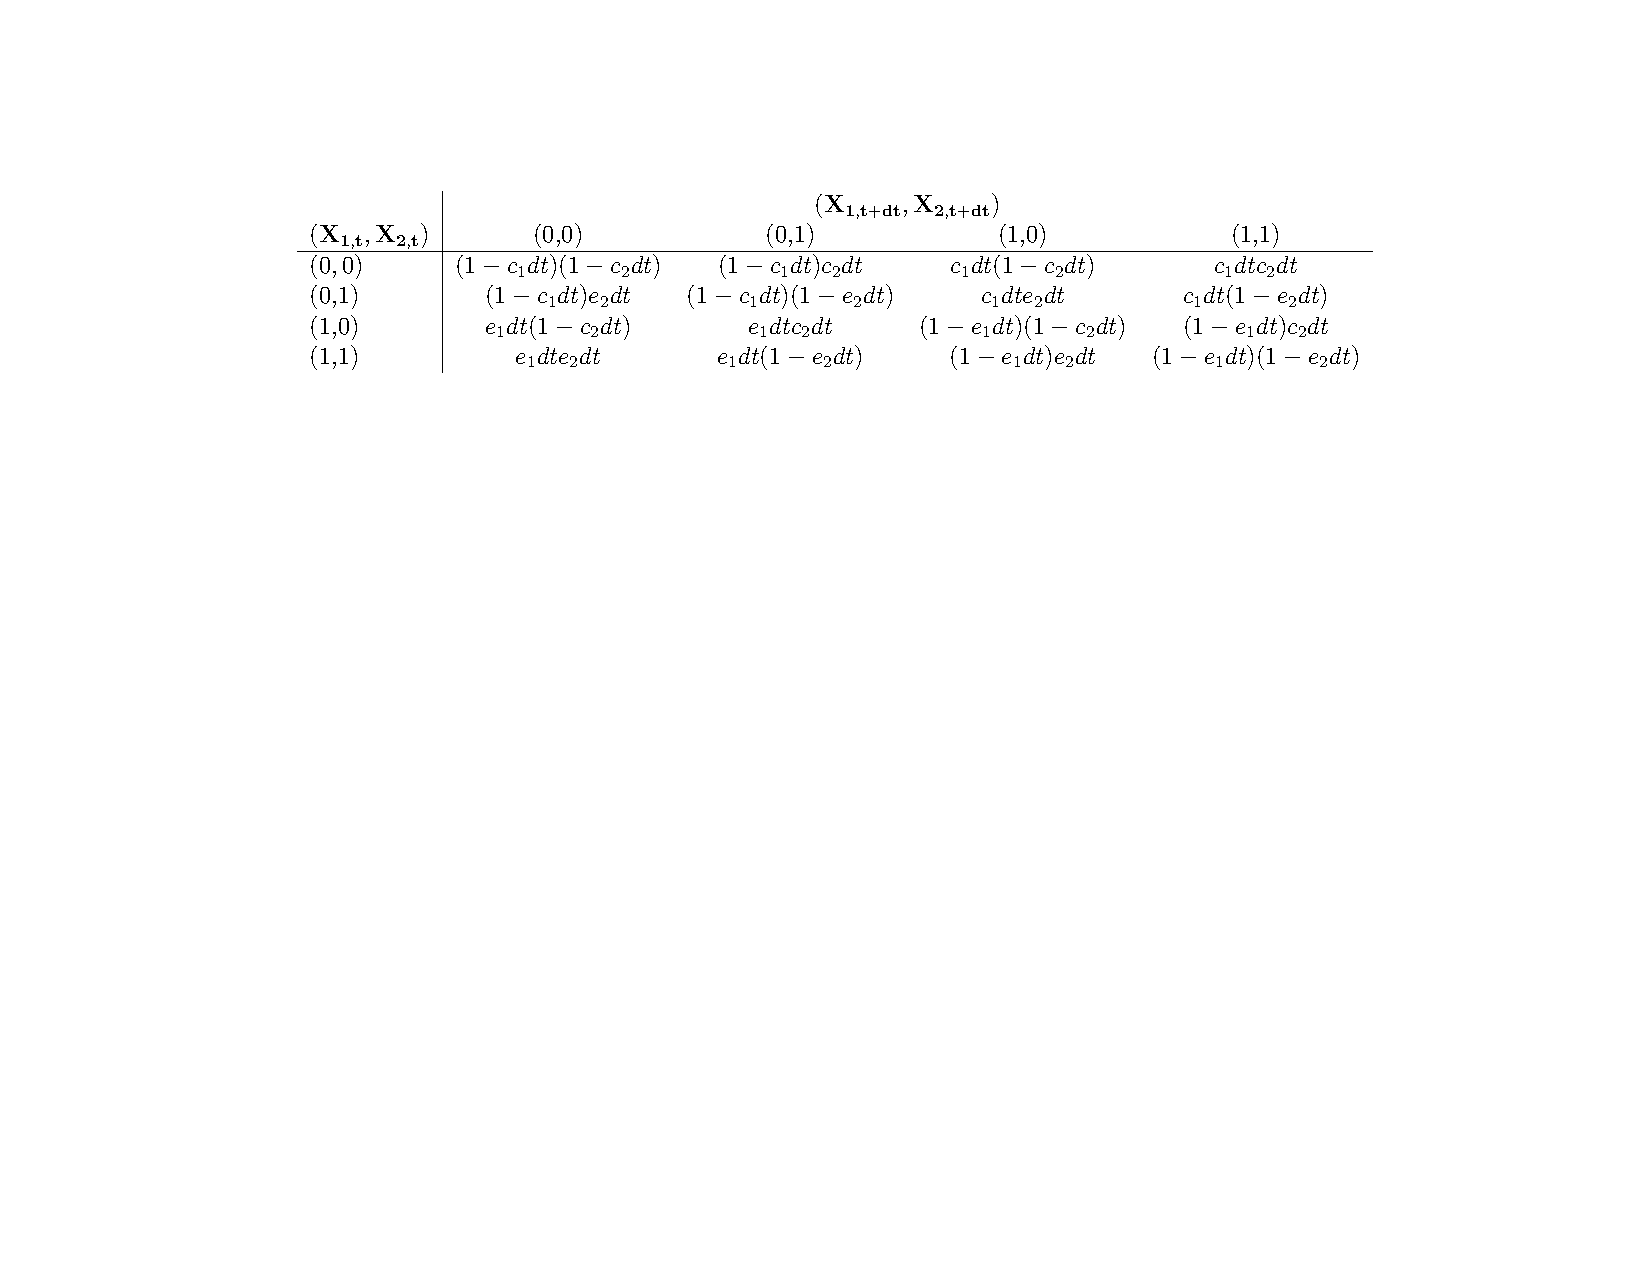
\includegraphics[scale=0.85]{./chapitre1/table1.pdf}
\caption{}
\label{tb1}
\end{table}



--------------------------------------------------------------
\section{Figures}


\subsubsection*{Figure 1}
%-------------------------
\begin{figure}[h!]
\centering
\includegraphics[width=\textwidth]{./chapitre1/fig1.eps}
\caption{}
\label{fig1}
\end{figure}
%
% \newpage
%
%
\subsubsection*{Figure 2}
%-------------------------
\begin{figure}[h!]
\centering
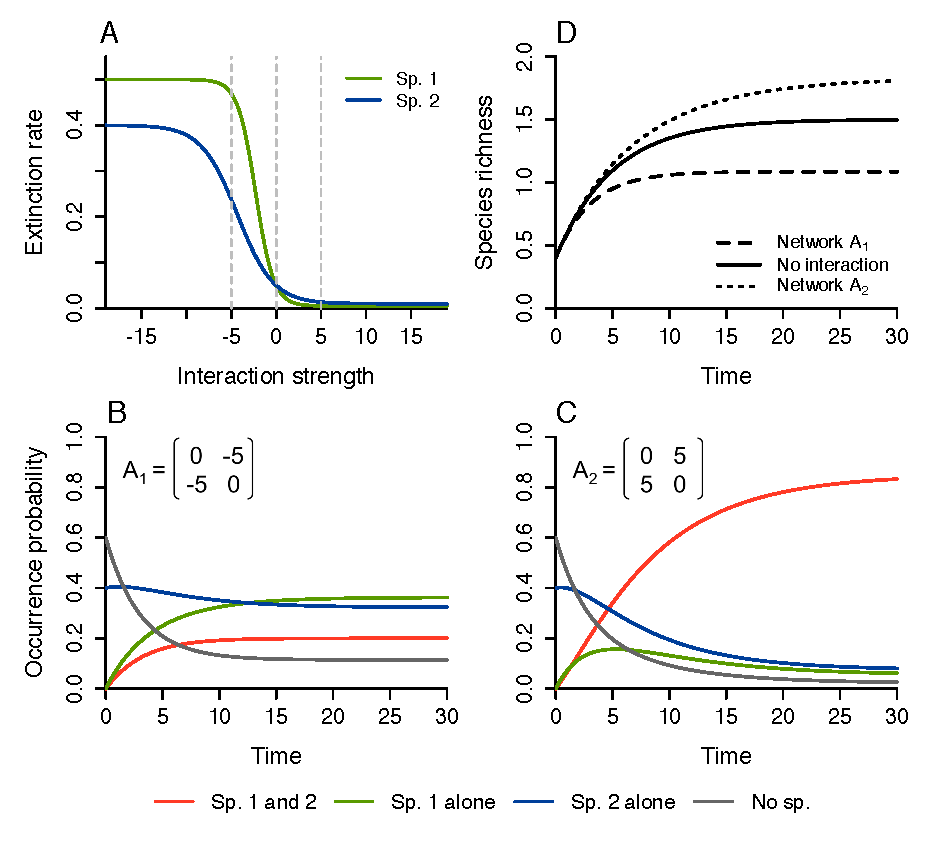
\includegraphics[width=\textwidth]{./chapitre1/fig2.eps}
\caption{}
\label{fig2}
\end{figure}

\newpage
%

\subsubsection*{Figure 3}
%-------------------------
\begin{figure}[h!]
\centering
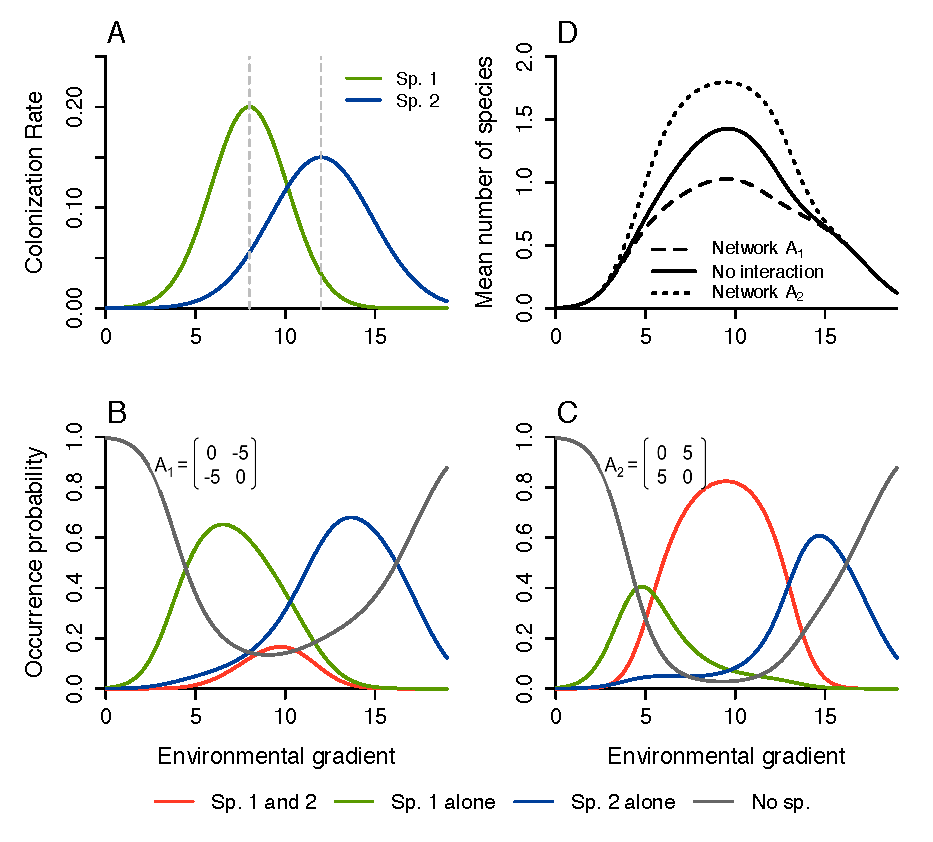
\includegraphics[width=0.8\textwidth]{./chapitre1/fig3.eps}
\caption{}
\label{fig3}
\end{figure}

\newpage

%
\subsubsection*{Figure 4}
%-------------------------
\begin{figure}[h!]
\centering
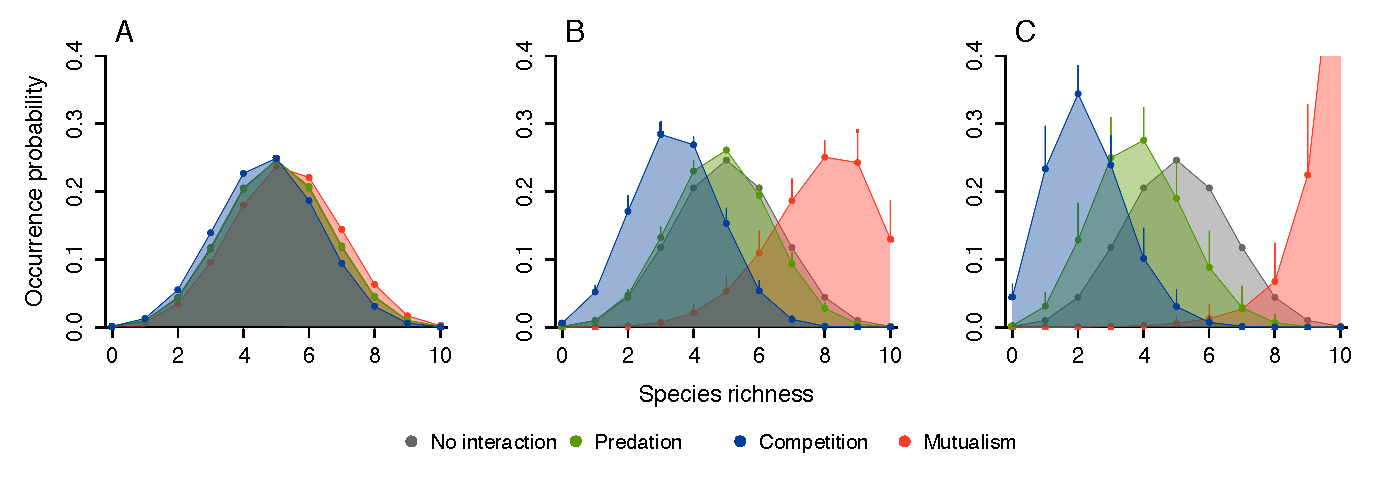
\includegraphics [width=\textwidth]{./chapitre1/fig4.eps}
\caption{}
\label{fig4}
\end{figure}

\newpage

%
\subsubsection*{Figure 5}
%-------------------------
\begin{figure}[h!]
\centering
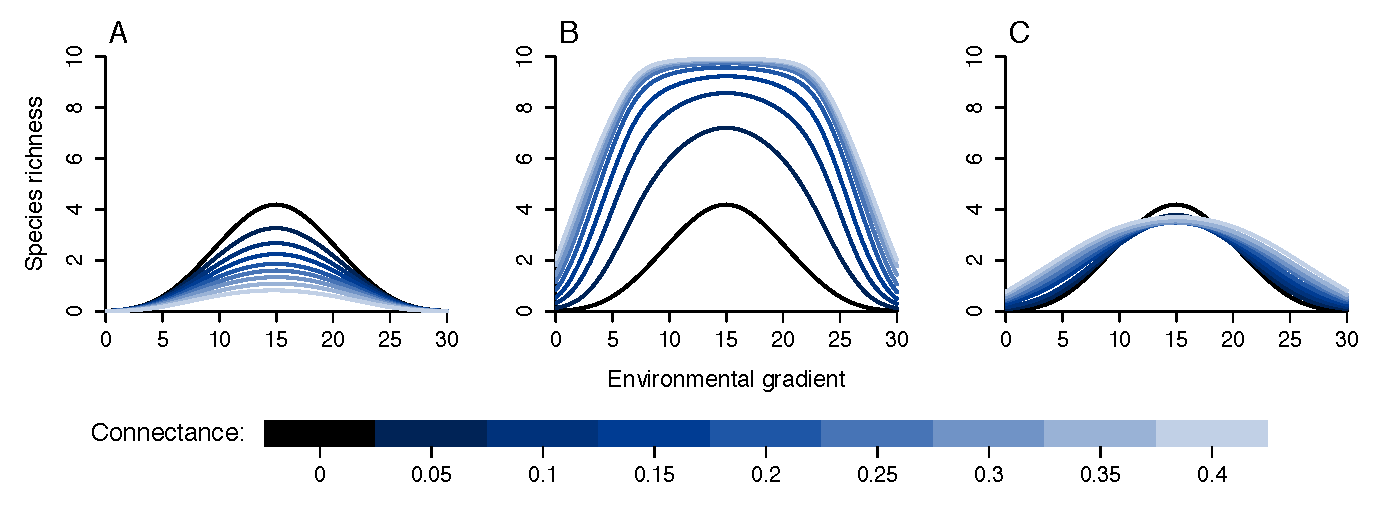
\includegraphics [width=\textwidth]{./chapitre1/fig5.eps}
\caption{}
\label{fig5}
\end{figure}

\chapter{THEORIE DE CO-OCCURRENCE DES ESPECES DANS LES RÉSEAUX D'INTERACTION}


\section{Résumé en français du deuxième article}

Dans le chapitre précédent, nous avons mis en évidence l'impact potentiel des interactions sur la présence locale des espèces dans le cadre de la théorie de la biogéographie des îles. Nous avons ainsi mis en évidence un effet des interactions sur la répartition géographique des espèces. Nous avons proposés une solution efficace pour essayer d'inclure ces interactions : ne pas traiter les espèce une à une mais les utiliser sous forme d'assemblage. Cette approche a déjà une place importante dans la litérature en biogéographie sous la forme des diverses approches de modélisation à l'échelle des communautés. Dans ces approches, il existe toujours une étape au cours de laquelle les différentes espèces sont assemblées en vue d'améliorer les prédictions de biodiversité. Seulement, ces méthodes ne font pas de lien entre les interactions et ces assemblages qui demeurent des groupes d'espèce trouvés fréquemment ensemble. Pour montrer l'importance des intéractions dans les modèles en biogéographie, nous nous sommes intéressés à leur impact sur une mesure majeure en biogéographie : la co-occurrence.

La co-occurence de deux espèces est simplement le nombre total de sites où les espèces sont présentes ensemble rapporté au nombre totale de sites étudiés. Pour pouvoir allez plus loin, nous avons défini une mesure de co-occurence sous l'hypothèse d'indépendance de deux espèces. Cela signigfie simplement que nous prenons l'occurrence respective des deux espèces et que nous les mulitplions pour obetnir notre seconde mesure. Grâce à la comparaison entre ces deux valeurs nous avons pu illustrer, dans l'article présenté ci-dessous, cinq grands principes relatifs à la co-occurence des espèces en interaction :

1. \textbf{Les interactions directes entre deux espèces affectent leur probabilité de co-occurence}. C'est une transposition directe du chapitre précédent sur la mesure de co-occurrence : s'il existe un lien entre deux espèces, leur probabilité d'être présente simultannément dans une localité différe de la probabilité attendue si elle se recontrait aléatoirement.

2. \textbf{Les interactions indirectes modifient leur probabilité de co-occurence}. Malgrè qu'il n'existe pas d'interaction directe entre deux espèces, ces dernières peuvent néanmoins être liées par une ou plusieurs autres espèces, l'interaction est dite indirecte. Si les conséquence des interactions directes se propagent propager à travers le réseau via ces relations indirectes, il est alors possible que répartition d'une espèce soit affectée par une autre espèce avec laquelle aucune interaction directe n'est constatée.

3. \textbf{L'effet des interactions sur la co-occurrence n'est pas symétrique}. Il n'existe a priori aucune raison pour que ces effets soient symétriques. Néanmoins en utilisant la mesure de co-occurrence telle que décite ci-dessus, nous la considérons comme telle. Nous montrons alors comment les probabilités conditionnelles peuvent prendre en compte l'asymétrie des effets des interactions.

4. \textbf{La force d'association entre deux espèces diminue avec la longueur du plus court chemin entre deux espèces}. Plus les espèces sont éloignées dans le réseau, moins les conséquences des interactions indirectes seront perceptibles, nous illustrons donc que les effets des interactions directes diminuent lors de leur propagations dans le réseau.

5. \textbf{La force d'une association avec une autre espèce diminue avec le nombre d'inetraction qu'elle entretient.} Si une espèce a de nombreux liens dans le réseau (par exemple, un prédateur généraliste), alors celle-ci sera moins dépendante d'une espèce en particulier et de fait la relation qu'elle entretien avec les expèces se rapprochera de la co-coorrence sous hypothèse d'indépendance.


Pour ce second papier, le contexte est particulier : Dominique Gravel a été invité à un numéro spécial de \textit{Theoritical Ecology}. Dominique Gravel m'a alors proposé de travailler sur le prolongement de la reflexion mené au premier chapitre et de l'appliquer sur les données de co-occurrence. J'ai alors conceptualisé un modèle probabiliste pour tenter de comprendre comment les interactions peuvent affecter la co-occurrence. Je me suis occupé de toute la partie modèle et des figures. Dominique Gravel a écrit la majeure partie de l'introduction et de la discussion. La reflexion mené ayant été entammé par Dominique Gravel et  Miguel B. Ara\'ujo, ce chercheur est devenu second auteur et à participer activement à la rédaction. Enfin, Nicolas Mouquet a participé substentiellement à la rédaction du manuscript.



\newpage

\section{TITLE}

A Theory for species co-occurrence in interaction networks

\section{AUTHORS}

Kévin Cazelles, Miguel Ara\'ujo, Nicolas Mouquet et Dominique Gravel

\section{ABSTRACT}

The study of species co-occurrences has been central in community ecology since the foundation of the discipline. Co-occurrence data are, nevertheless, a neglected source of information to model species distributions and biogeographers are still debating about the impact of biotic interactions on species distributions across geographical scales. We argue that a theory of species co-occurrence in ecological networks is needed to better inform interpretation of co-occurrence data, to formulate hypotheses for different community assembly mechanisms, and to extend the analysis of species distributions currently focused on the relationship between occurrences and abiotic factors. The main objective of this paper is to provide the first building blocks of a general theory for species co-occurrences. We formalize the problem with definitions of the different probabilities that are studied in the context of co-occurrence analyses. We analyse three species interactions modules and conduct multi-species simulations in order to document five principles influencing the associations between  species within an ecological network: i) direct interactions impact pairwise co-occurrence; ii) indirect interactions impact pairwise co-occurrence; iii) pairwise co-occurrence rarely are symmetric; iv) the strength of an association decreases with the length of the shortest path between two species; v) the strength of an association decreases with the number of interactions a species is experiencing. Our analyses reveal the difficulty of the interpretation of species interactions from co-occurrence data. We discuss whether the inference of the structure of interaction networks is feasible from co-occurrence data. We also argue that species distributions models could benefit from incorporating conditional probabilities of interactions within the models as an attempt to take into account the contribution of biotic interactions to shaping individual distributions of species.

\section{KEYWORDS}

Co-occurence, Ecological networks, Biogeography, Indirect interactions, Null models


\section{Introduction}
\label{intro}

Understanding of the processes driving the assembly of communities has been a central theme of ecology since the foundation of the discipline. How do we start from a regional species pool to assemble a structured community? Why are some species associated with each other? The work of \cite{Diamond1975Assembly} pioneered the analysis of species co-occurrence in geographical space and, together with the controversy triggered by
\cite{Connor1979Assembly}, it stimulated the development of a new field of
research in numerical ecology (\citealt{Stone1990Checkerboard, Gotelli1996Null,
Legendre2012Numerical}). The foundational work on species co-occurrences also led to the development of a rich array of methodological tools designed to test null hypotheses in ecology. Even if null models could be achieved numerically (e.g., \cite{Araujo2011Using}), typically they are based on permutations of distribution data. Null models have been used to infer the role of biotic interactions between pairs of species on their individual distributions. Studying the different drivers of species co-occurrence is not only of theoretical interest for improving understanding of the mechanisms of community assembly. It is also instrumental in predictive ecology, because a considerable amount of information is contained in species distributions data.

Despite its historical importance for community ecology, co-occurrence data remain a neglected source of information in models of species distributions. Biogeographers are still debating the impact of biotic interactions on species distributions (\citealt{Guisan2005Predicting, Gotelli2010Macroecological,
Kissling2011Towards,Pellissier2013Combining}). The distribution of a species
is thought to be first influenced by its physiological tolerance to
environmental conditions, but also by interactions with other species
(\citealt{Hutchinson1957Concluding, Macarthur1972Geographical,
Peterson2011Ecologicala, Boulangeat2012Accounting}). The question of whether such
interactions leave imprints in the distributions of individual species at
biogeographical scales is still open to debate (\textit{e.g.}
\citealt{Davis1998Making}), but recent empirical
\citealt{Gotelli2010Macroecological}, modeling (\textit{e.g.}
\citealt{Araujo2007Importance}), and theoretical (\citealt{Araujo2011Using})
evidence invites the interpretation that this might indeed be the case.

The overwhelming majority of species distributions modelling applications, nonetheless, neglect information contained in joint distributions. Even multivariate analysis of community data (\textit{e.g.} redundancy analysis - (\citealt{Legendre2012Numerical}) do not use co-occurrence in geographical space to condition individual species response to environmental variation.  There has been a recent rise of interest however in joint species distribution modelling (\citealt{Clark2014More, Harris2015Estimating, Pollock2014Understanding}). These methods estimate the distribution of all species from a pool simultaneously and allow to condition the presence of a species on all other ones. However, estimated relationships are inferred from co-occurrence in environmental space rather than geographical space. That is, joint responses to the environment are inferred rather than biotic interactions themselves (\citealt{Baselga2009Individualistic}). JSDMs are, nonetheless, a first step towards developing a next generation of models accounting for the impact of biotic interactions on the distributions of species. They are, however, purely empirically driven and carry no specific hypotheses about how interactions can affect distributions. An exception is the recent attempt to model the effects of predator-prey dynamics on distributions and abundances using a meta- community framework coupled with phenomenological species distributions models (\citealt{Fordham2013Adapted}). The problem with such approaches is that data to parametrize interactions mechanistically are generally lacking (\citealt{Castilla2015Inferring}); therefore, they are hardly applied in most circumstances. It follows that we are faced with at least two major problems: i) understanding of the ecological interactions underlying the distributions of species is limited; and ii) knowledge of interactions is typically limited to net interactions, mixing both direct and indirect interactions. A theory of species co-occurrences in ecological networks is, therefore, needed to help interpret co-occurrence data, to formulate hypotheses for different community assembly mechanisms, and to extend the analysis of species distributions currently focused on the relationship between occurrences and abiotic factors.

The analysis of species co-occurrences starts with a matrix representing the presence and absence of each species over a set of sites. There are two aspects to the quantitative study of co-occurrence. The first is the choice of the metric used to quantify the strength of associations (relationships between species occurrences) between pairs of species. The simplest measure of species co-occurrence is the number of species combinations, as defined by \cite{Pielou1968Association}. A second
index is the count of checkerboards \cite{Diamond1975Assembly}: ``In such a
pattern, two or more ecologically similar species have mutually exclusive but
interdigitating distributions in an archipelago, each island supporting only
one species'' (p. 32). Another popular index of co-occurrence is the C-score
(\citealt{Stone1990Checkerboard}). This index is similar to the count of
checkerboards; it measures the average association or repulsion between pairs
of species.

The second aspect of the analysis of species co-occurrence is the formulation of a null model. The controversy generated in \cite{Connor1979Assembly} was partly (and rightly) based on the absence of a valid null hypothesis in Diamond’s analysis. Subsequent debates were mostly concerned with the formulation of the null hypothesis (e.g.,
\citealt{Diamond1982Examination}). Thanks to the theoretical work of
\cite{Gotelli1996Null}, there is now a clear understanding of the different
null models that can be constructed from the community matrix. New indices are
constantly proposed, such as in (\citealt{Boulangeat2012Accounting, Veech2013Probabilistic}; see also Table 2 in \citealt{Ulrich2013Pattern} for a description of 15 indices for co-occurrence analysis). A promising avenue is the one proposed by
\cite{Araujo2011Using} for the study of the matrix of species co-occurrence
with tools borrowed from network theory.

Surprisingly, there is currently no theory for co-occurrence in multi-species communities. The basic hypotheses are that pairwise negative interactions result in repulsion, while pairwise positive interactions result in attraction. Attraction and repulsion are assessed by a comparison of the number of co-occurrence events to the number expected under a totally independent distribution. Similar environmental requirements between species could also result in attraction, even in the absence of interactions, if the sampling is conducted across heterogeneous environmental conditions. This theory is limited to pairwise and symmetric interactions; there is nothing for antagonistic and indirect interactions. Food web ecologists were among the first to recognize the important effect of indirect interactions on abundance
(\citealt{Wootton1994Nature}). For instance, plant and carnivore abundances are expected to correlate across a productivity gradient
(\citealt{Hairston1960Community, Oksanen1981Exploitation}) because of top-down control on the herbivore population. Similarly, the propagation of indirect interactions has been studied in more complex interaction networks (\citealt{Yodzis1988Indeterminacy}). Indirect interactions could reverse the net interaction in a surprising way, such that predator-prey abundances could be positively related (\citealt{Montoya2009Press}). Empirical analysis of co-occurrence for several taxa has shown that they are usually asymmetric (Araújo et al. 2011), such that a species distribution tended to be nested within the distribution of other (\textit{e.g.} predator-prey distributions; \citealt{Holt2009Trophic, Gravel2011Trophic}). In such a case, even if the co-distribution signature is quite understood, available methods will likely fail at using this piece of information to improve forecasts.


The main objective of this paper is to provide the first building blocks of a general theory of species co-occurrences. We formalize the proposed theory with definitions of different quantities that are studied in the context of co-occurrence analyses. Herewith, we analyse three species interactions modules in order to document five principles influencing the association between pairs of species from an ecological network:
i) direct interactions impact pairwise co-occurrence;
ii) indirect interactions impact pairwise co-occurrence;
iii) pairwise co-occurrence does not have to be symmetric;
iv) the strength of an association decreases with the length of the shortest path between two species;
v) strength of an association decreases with the number of interactions a species is experiencing.
We base our mathematical argument on a general model of species distributions that is free of
any assumption about how the ecological interactions operate. Finally we
extend our analysis with simulations of multi-species networks in order to
analyse how these mechanisms scale up in species rich communities.



%---------------------------------------------
\section{Definitions}
\label{def}


We start with definitions to formalize the quantities that can be computed
from species distribution data and be used in the context of co-occurrence
analyses. Let $X_i$ be the random variable representing the presence of species
$i$. $X_i=1$ when species $i$ is present, $X_i=0$ otherwise. Then $X_{i,t>0}$ is
the random process associated, giving the value that $X_{i,t}$ takes at any time
$t$. Let $p_{i,t}$ standing for the probability $\mathbb{P}(X_{i,t}=1)$. Also, to illustrate the defintions, we derive the quantities for a simple presence/absence dataset (see Table \ref{tab:2}).

The \textbf{marginal occurrence probability} $\mathbb{P}(X_{i,\infty}=1)=p_i^*$
represents the occurrence probability of species $i$ when the system is at
equilibrium, in the sense of the classical theory of island Biogeography \cite{Macarthur1967Theory}. As we assume so for all species, we drop the $*$ and the $\infty$ for the sake of clarity. The marginal occurrence probability is the sum of the occurrence of the species across all possible set of species in the data. In other words, it corresponds to the sum of the column of the site $\times$ species table, divided by the total number of sites
$N$. Marginal occurrence probabilities for species in Table \ref{tab:2} are: $p_1=0.6$, $p_2=0.6$ and $p_3=0.4$.

The \textbf{observed co-occurrence} between species $i$ and $j$ is
the joint probability $p_{i,j}=\mathbb{P}(X_{i}=1 \cap X_{j}=1)$. It represents the
number of sites where the two species are found together, across all possible
set of species in the data (in other words, it is a marginal probability
with respect to other species), divided by $N$. In our dataset, for instance, we have $p_{1,2}=0.3$ and $p_{1,3}=0.2$.

The \textbf{conditional co-occurrence} between species $i$ and $j$ is
$p_{i|j}=\mathbb{P}(X_{i}=1| X_{j}=1)$. It represents the probability of
observing species $i$, knowing that species $j$ is already present. This
quantity is close to the measure of association between two
species because it is independent of the marginal occurrence probability of
both species. The problem is that, as soon as there are other species present,
the conditional co-occurrence as expressed here is marginalized over the set
of all other species from the community $K$. For instance, for three species, we have:
 $p_{1|2} = \mathbb{P}(X_{1}=1| X_{2}=1,X_{3}=1) + \mathbb{P}(X_{1}=1| X_{2}=1,X_{3}=0)$.
It, therefore, includes both the effect of \emph{direct} and \emph{indirect} associations between species, e.g. the direct association of species 1 with species 2 or the indirect association of species 3 with 1 via its effect on 2.
Consequently, the measure of pairwise association should be: $p_{i|j,\overline{K}}=\mathbb{P}(X_{i}=1| X_{j}=1,X_{K}=0)$,
where the horizontal bar over $K$ denotes absence of all other species. We
name this the \textbf{fundamental conditional co-occurrence}. For instance, in Table \ref{tab:2}, we get $p_{1|2}=\frac{p_{1,2}}{p_2}=0.5$ and $p_{1|2,\overline{3}}=\frac{p_{1,2,\overline{3}}}{p_{2,\overline{3}}}=\frac{0.2}{0.3}=0.67$.

Following the same logic, we define the \textbf{fundamental occurrence} as
$p_{i|\overline{K}}=\mathbb{P}(X_{i}=1| X_{K}=0)$. The fundamental occurrence
is conceptually equivalent to the fundamental niche of Hutchinson (1957) and
represents the probability of observing a species in the absence of biotic interactions,
i.e., when all other species are absent.
 By analogy, the marginal occurrence should be interpreted as the
realized distribution. For species 1 in Table \ref{tab:2} we calculate $p_{1|\overline{23}}=\frac{p_{1,\overline{2},\overline{3}}}{p_{\overline{2},\overline{3}}}=\frac{0.2}{0.3}=0.67$.

Finally, we define the \textbf{independent co-occurrence} as
$p_{i,j;IND}=\mathbb{P}(X_{i}=1)\mathbb{P}(X_{j}=1)$. It represents the
co-occurrence between any pairs of species expected in absence of any
association between them. In ecological terms, it would represent the
co-occurrence when ecological interactions and habitat filtering do not impact
species distribution. It also represents the null model against which
observed co-occurrence is usually compared to. Note the independent
co-occurrence is different from the one expected under a neutral model
(\citealt{Hubbell2001Unified}). Firstly because strong competitive interactions in
the neutral model forces repulsion and, secondly, because dispersal limitation
also causes spatial aggregation and thus a non-random distribution of
co-occurrence (\citealt{Bell2005CoDistribution}). In our example, we obtain, for instance, $p_{1,2;IND}=0.36$ and $p_{2,3;IND}=0.24$.

%---------------------------------------------
\section*{Direct association between two species}
\label{direct}

We start with the analysis of a two species situation, labeled species $1$ and
species $2$, in order to understand direct associations between species pairs. A
third species, $3$, will be introduced in the next section to study indirect
associations. The model we develop is general, as we do not specify the type of
ecological interactions involved. It therefore accounts for all possible mechanisms from
which an association between a pair of species could arise, such as trophic
interactions involving energy fluxes, non-consumptive interactions, parasitism,
direct interference, territoriality, space pre-emption, niche construction,
etc. The impact of predator-prey interactions in a metapopulation setting with
colonization and extinction dynamics will be considered for the multi-species
simulations.

As we are willing to understand the role played by interactions in co-occurrence, we start by defining marginal co-occurrence probabilities of our two species by a decomposition into conditionnal co-occurrences. By the formula of total probability we have:

%%--------
  \begin{eqnarray} \label{s2ind}
    \nonumber p_1&=& \mathbb{P}(X_{1}=1\cap X_{2}=1)+ \mathbb{P}(X_{1}=1\cap X_{2}=0)\\
    \nonumber \label{sp2ind} &=& \mathbb{P}(X_{1}=1| X_{2}=1)\mathbb{P}(X_{2}=1) \\
    &&+ \mathbb{P}(X_{1}=1| X_{2}=0)\mathbb{P}(X_{2}=0)
  \end{eqnarray}
%%--------

We do the same for species 2. Using the notation described above, \eqref{s2ind} could be rewritten as:

%%--------
  \begin{equation}
    \label{s2nind}
    \left\{ \begin{aligned}
      p_1&= p_{1|2}p_2+p_{1|\overline{2}}(1-p_2) \\
      p_2&= p_{2|1}p_1+p_{2|\overline{1}}(1-p_1)\\
    \end{aligned} \right.
  \end{equation}
%%--------

where the vertical bar denotes the absence of a species. By solving the latter system,
we get:

%%--------
  \begin{equation} \left\{ \begin{aligned} \label{sol2}
    p_1=&  \frac{p_{1|\overline{2}}+ p_{2|\overline{1}} (p_{1|2}- p_{1|\overline{2}})}{1- (p_{2|1}-p_{2|\overline{1}})( p_{1|2} - p_{1|\overline{2}})} \\
    p_2=& \frac{p_{2|\overline{1}}+p_{1|\overline{2}} (p_{2|2}- p_{2|\overline{1}})}{1- (p_{2|1}-p_{2|\overline{1}})( p_{1|2} - p_{1|\overline{2}})}
  \end{aligned} \right. \end{equation}
%%--------

When species are independent, we have $p_{1|\overline{2}}=p_{1|2}=p_1$ and
$p_{2|\overline{1}}=p_{2|1}=p_2$, then we logically find \eqref{s2ind} again. Then, we can deduce
the following interpretation of the impact of \textbf{direct interactions} on co-occurrence:

%%--------
  \begin{itemize}
    \item[i] if species $1$ cannot persist in absence of $2$ (e.g., a parasite requiring its host), then $p_{1|\overline{2}} \rightarrow 0$, therefore $p_1 \rightarrow p_{1|2}p_2$

    \item[ii] if species $1$ depends strongly on 2 thereby perfect­ly tracking its distribution $2$, the $p_{1|\overline{2}} \rightarrow 0$ and $p_{1|2} \rightarrow 1$, and therefore $p_1 \rightarrow p_2$

    \item[iii] if species 2 excludes 1, then $p_{1|2} \rightarrow 0$ and $p_{2|1} \rightarrow 0$ , so $p_1=\frac{p_{1|\overline{2}}-p_{2|\overline{1}}p_{1|\overline{2}}}{1-p_{2|\overline{1}}p_{1|\overline{2}}}$ and $p_2=\frac{p_{2|\overline{1}}-p_{2|\overline{1}}p_{1|\overline{2}}}{1-p_{2|\overline{1}}p_{1|\overline{2}}}$. Therefore, if $p_{1|\overline{2}} \rightarrow 1$, then $p_1\rightarrow1$ and $p_2\rightarrow0$.

  \end{itemize}
%%--------

%---------------------------------------------
  \section*{Co-occurrence in three-species modules}
  \label{3spcooc}

Now, we consider the co-occurrence between three species. We start with a
general derivation of co-occurrence and then interpret the results for
particular modules in order to reveal fundamental principles underling co-occurrence in
ecological networks. Our solution provides insights to decipher the solution
of species-rich networks since the three-node connected subgraphs are
fundamental building blocks of larger networks (\citealt{Milo2002Network,
Stouffer2007Evidence, Stouffer2010Understanding}). We use the same approach as in \eqref{sp2ind} and get the subsequent equation:

%%--------
  \begin{eqnarray} \label{sp3p1}
    \nonumber p_1&=& \mathbb{P}(X_{1}=1\cap X_{2}=1\cap X_{3}=1) +  \mathbb{P}(X_{1}=1\cap X_{2}=0\cap X_{3}=1) \\
      &&+ \mathbb{P}(X_{1}=1 \cap X_{2}=1 \cap X_{3}=0)+ \mathbb{P}(X_{1}=1 \cap X_{2}=0 \cap X_{3}=0)
      % &=& \left( \mathbb{P}(X_{1}=1\cap X_{2}=1 | X_{3}=1)+\mathbb{P}(X_{1}=1\cap X_{2}=0 | X_{3}=1) \right) \mathbb{P}(X_{3}=1) \\
      % &&+ \left( \mathbb{P}(X_{1}=1\cap X_{2}=1 | X_{3}=0)+\mathbb{P}(X_{1}=1\cap X_{2}=0 | X_{3}=0) \right) \mathbb{P}(X_{3}=0)
  \end{eqnarray}
%%--------

% In order take advantage from our previous results, we note that

As $\{X_{3}=1,X_{3}=0\}$ forms a partition we get:

%%--------
  \begin{eqnarray} \label{sp3p1b}
    p_1&=& \mathbb{P}(X_{1}=1| X_{3}=1)p_3 + \mathbb{P}(X_{1}=1| X_{3}=0)(1-p_3)
  \end{eqnarray}
%%--------

This equation is analogous to the two-species interactions equation but enables the study of networks involving three species interactions, with species 2 being hidden by marginalization. We split the three species problem in two distinct two-interactions species problems. Firstly, we solve the equation for sites without species 3 and get:

%%--------
  \begin{eqnarray}
    \label{sols2}
     p_{1|\overline{3}}=\mathbb{P}(X_{1}=1| X_{3}=0)&=& \frac{p_{1|\overline{2}\overline{3}}+ p_{2|\overline{1}\overline{3}} (p_{1|2\overline{3}}- p_{1|\overline{2}\overline{3}})}{1- (p_{2|1\overline{3}}-p_{2|\overline{1}\overline{3}})( p_{1|2\overline{3}} - p_{1|\overline{2}\overline{3}})}
 \end{eqnarray}
%%--------

which is similar to equation \eqref{sol2} but with an explicit absence of species 3. We do similarly for the conditional occurrence of 1 on species 3:

%%--------
  \begin{eqnarray}
     \label{sols2b}
     p_{1|3}=\mathbb{P}(X_{1}=1| X_{3}=1)&=& \frac{p_{1|\overline{2}3}+ p_{2|\overline{1}3} (p_{1|23}- p_{1|\overline{2}3})}{1- (p_{2|13}-p_{2|\overline{1}3})( p_{1|23} - p_{1|\overline{2}3})}
  \end{eqnarray}
%%--------

Doing so, we get the following set of equations describing the marginal occurrence probabilities for the three species:

%%--------
  \begin{equation} \left\{ \begin{aligned} \label{s3nind}
    p_1 &=&  p_{1|3}p_3 + p_{1|\overline{3}}(1-p_3)  \\
    p_2 &=& p_{2|3}p_3 + p_{2|\overline{3}}(1-p_3)  \\
    p_3 &=&  p_{3|2}p_2 + p_{3|\overline{2}}(1-p_2)
  \end{aligned} \right. \end{equation}
%%--------

Note that we could have chosen a different set of equations depending on the way we split the problem, for instance, we could have started by considering the occurrence of species 1 given the occurrence of species 2 instead of species 3. Now, we solve the above linear system of three equations with three unknowns and find that:
%DG: explain how you do solve the problem (incorporating wich equation into which)

%%--------
\begin{equation} \left\{ \begin{aligned} \label{sol3}
    p_1 =& \frac{p_{1|\overline{3}}+p_{3|\overline{2}}(p_{1|3}-p_{1|\overline{3}})+(p_{3|2}-p_{3|\overline{2}})(p_{1|3}p_{2|\overline{3}} -p_{1|\overline{3}}p_{2|3})}  {1-(p_{2|3}-p_{2|\overline{3}})(p_{3|2}-p_{3|\overline{2}})}\\
    p_2 =& \frac{p_{2|\overline{3}}+p_{3|\overline{2}}(p_{2|3}-p_{3|\overline{2}})}{1-(p_{2|3}-p_{2|\overline{3}})(p_{3|2}-p_{3|\overline{2}})} \\
    p_3 =& \frac{p_{3|\overline{2}}+p_{2|\overline{3}}(p_{3|2}-p_{3|\overline{2}})}{1-(p_{2|3}-p_{2|\overline{3}})(p_{3|2}-p_{3|\overline{2}})}
  \end{aligned} \right. \end{equation}
%%--------

Conditional probabilities of the right-hand sides can all be derived as we did for $p_{1|3}$ in equation \eqref{sols2b}.



\subsection*{Community modules}
\label{modules}

We now interpret these equations with examples of well-studied food web modules in
community ecology: 1) linear food chain, 2) exploitative competition and 3)
apparent competition. To do so, we consider matrices of direct
associations representing the conditional co-occurrence probabilities among all
pairs of species (see Table \ref{tab:1}).

We are interested by the \emph{observed co-occurrence} because this is the quantity that is easily measurable from species distributions data, thus being the one that is typically studied. We consider that the marginal occurrence is also a known quantity and, therefore, we examine the effect of particular conditional co-occurrence arrangements on observed co-occurrences. We will not provide derivations for each module, but focus on particular pairs to illustrate two of the five principles.

\paragraph{Indirect interactions}. The comparison between the observed
co-occurrence and the conditional co-occurrence reveals the role of indirect
interactions on species associations. Based on \eqref{sol3} and \eqref{sols2}
we get the association between species $i$ and $k$:

%%--------
\begin{eqnarray}
  \nonumber p_{i,k} &=& p_i-p_{i,\overline{k}}(1-p_k) \\
  p_{i,k}&=& p_i-\frac{p_{i|\overline{jk}}+ p_{j|\overline{ik}} (p_{i|j\overline{k}}- p_{i|\overline{jk}})}{1- (p_{j|i\overline{k}}-p_{j|\overline{ik}})( p_{i|j\overline{k}} - p_{i|\overline{jk}})}(1-p_k)
\end{eqnarray}
%%--------

Therefore the observed co-occurrence between species i and k depends on their
respective interaction with species j
($p_{j|\overline{ik}}$,$p_{j|i\overline{k}}$ and $p_{j|\overline{ik}}$). The
conditional co-occurrence between two species could be null, but their
observed co-occurrence be non-independent because of a shared interaction.
This principle is best illustrated by the co-occurrence between a carnivore
and a plant (species 3 and 1, respectively) in a linear food chain. In
this situation, according to Table \ref{tab:1}, we find that the observed co-occurrence
between the plant and the carnivore is:

%%--------
\begin{equation} \label{linear}
  p_{1,3} = p_1-\frac{p_{1|\overline{2}\overline{3}}}{1-p_{2|1\overline{3}}( p_{1|2\overline{3}} - p_{1|\overline{2}\overline{3}})}(1-p_3)
\end{equation}
%%--------

It is clear from this equation that there is a significant association between
the carnivore and the plant, despite the conditional co-occurrence of the two
species being totally independent. The indirect association gets stronger with
the strenght of both conditional co-occurrence.

Similar observations could be made by studying the observed co-occurrence between
consumers (species 2 and 3) in the exploitative competition module:

%%--------
\begin{equation} \label{exploitative}
  p_{2,3} = p_2-\frac{p_{1|\overline{2}\overline{3}}p_{2|1\overline{3}}}{1- (p_{1|2\overline{3}}-p_{1|\overline{2}\overline{3}})p_{2|1\overline{3}}}(1-p_3)
\end{equation}
%%--------

And between resources in the apparent competition module (species 1 and 2):

%%--------
\begin{equation} \label{apparent}
  p_{1,2} = p_1-\frac{p_{1|\overline{2}\overline{3}}}{1- p_{3|1\overline{2}}( p_{1|\overline{2}3} - p_{1|\overline{2}\overline{3}})}(1-p_2)
\end{equation}
%%--------

\paragraph{Associations do not have to be symmetrical.} Many studies of co-occurrence assume pairwise associations to be symmetrical (but see
\citealt{Araujo2011Using, Boulangeat2012Accounting}). The reason is simple, usually the observed
co-occurrence is compared to the independent co-occurrence. These two metrics
of association are perfectly symmetrical. This information is providing us an
inappropriate interpretation of the effect of interactions on species
distribution. If we consider for instance the association between the two
consumers (species $2$ and $3$) competing for a single resource (species $1$),
we have the observed co- occurrence at \eqref{exploitative}, which is
symmetrical by definition. The proportion of the area occupied by species $2$
where species $3$ is also present is not however equivalent to the proportion
of the areas occupied by species $3$. Rephrasing the problem,we find that
using \eqref{sols2b} and \eqref{exploitative}, $p_{2,3}/p_{2}$ is not equal to
$p_{2,3}/p_{3}$. One species could have a stronger impact on the distribution
of the other one. Predator distribution for instance tends to be
nested within the distribution of the prey (\citealt{Gravel2011Trophic}), and
consequently the predator has a high conditional co-occurrence with the prey,
and alternatively the prey has a low conditional co-occurrence with the
predator.

% %---------------------------------------------
\section*{Multi-species simulations}
\label{multi}

Now we move to multi-species simulations of more complex networks to reveal the
last two principles of our theory. To do so, we run simulations of the model of
trophic island biogeography developped by \cite{Gravel2011Trophic}. The model
describes the occurrence of a $S$ species regional network. Species stochastically
colonize islands with probability $c$ and go extinct with probability $e$, as in
the original model of \cite{Macarthur1967Theory}. Interactions are introduced with
three additional assumptions: i) a consumer species could colonize an island
only if it has at least one prey present (for simplicity, we consider producers
to be resident permanently on the island); ii) a consumer species goes extinct
if it loses its last prey species and iii) the presence of at least one predator
species increases the extinction probability by $e_d$. The consequence of these
assumptions is a sequential build-up of the food web on the island, starting
with low trophic level species with a general diet. Small and isolated islands
promote selection in favor of the most generalist species. The predictions
converge to the classic island biogeography theory for highly connected regional
food webs and large and connected islands (details in \citealt{Gravel2011Trophic}).

As mentioned above, there is a strong dependence of the predator
occurrence on the presence of its preys. Alternatively, when $e_d$ is
sufficiently large, the preys will tend to avoid locations with the predator
present. We consequently expect a strong signature of the network of
interactions on the co-occurrence matrix. We are however concerned that
indirect associations could emerge, as exemplified with the analysis of three
species modules above, and thereby mask the signal of conditional co-occurrences.

We simulated complex networks from 5 to 100 species using the niche model of
food web structure (\citealt{Williams2000Simple}). The diversity of primary
producers was fixed at 2, and their niche position was drawn randomly between
0 and 1 according to a uniform distribution. We fixed connectance at $C =
0.1$. Colonization probability was set at $c = 0.1$, baseline extinction
probability at $e = 0.2$ and predator-dependent additional extinction
probability at $e_d = 0.2$. Simulations were run for $10^7$ time steps to
evaluate the conditional occurrence probabilities, and 100 replicated networks
were simulated for each level of species richness.

\paragraph{Distance decay of observed co-occurrence.} The distribution of
observed co-occurrence is illustrated for pairs of species separated by
different path lengths at Figure 1A. The observed co-occurrence is presented
as a function of the expected co-occurrence under the hypothesis of
independent distributions. The strongest associations (given by the distance
between the observed and the independent co-occurrence) are observed among
pairs of species directly interacting with each other. The variance of the
distribution reduces from direct to first order indirect interactions, and
from first-order to higher interactions. We conclude that indirect non-
independent co-occurrences are possible in complex networks, but their
magnitude decreases as the number of links between two nodes decreases. This
result is similar to the observation of a distance decay of indirect
interactions in food webs (\citealt{Berlow2009Simple}).

\paragraph{Strength of co-occurrence decreases with degree and species
richness.} We performed simulations with a gradient of species richness and
observed that the variance of observed co-occurrence also decreases with the
degree of a species, i.e. the number of direct interactions a species is experiencing (Fig. 1B). We illustrated the relationship between the
degree of a species and the observed co-occurrence for pairs of species with a
direct association (Fig. 1C). This phenomenon has the consequence that the
strength of observed co-occurrence reduces with species richness. The niche
model has a constant connectance (\citealt{Williams2000Simple}), which has for consequence an increase of the degree with species richness. We find that the strength of co-occurrence
decreases with the degree. This result is straightforward to interpret: the
more diverse are the interactions, the weaker the impact of each
pairwise direct interaction on the species distribution. Again, this result is
similar to the observation of a scaling relationship between pairwise
interactions and food web diversity (\citealt{Berlow2009Simple}).

%---------------------------------------------
\section*{Discussion}
\label{discussion}

%
We first develop a probabilistic species distribution model constrained by
biotic interactions using conditional probabilities of co-occurrence. We then illustrate five general principles underlying the impact of ecological interactions on co-occurrence and that should be considered for the formulation of a general theory of species co-occurrence. Two of them have been widely noted before: \textbf{i)} direct interactions affect species distributions and generate deviations in co-occurrences from that expected if distributions of species were independent from each other; \textbf{ii)} the effect of direct associations is often asymmetric, as envisioned in trophic metacommunity ecology (\citealt{Holt2009Trophic}). We also illustrate principles that have been overlooked in most studies of co-occurrence (\citealt{Araujo2011Using}); \textbf{iii)} indirect interactions generate deviate co-occurrence from expectation under independence assumption; \textbf{iv)} the strength of indirect associations decreases with the length of the shortest path distance between species pairs in a network; while \textbf{v)} also decreasing with the number of interactions a species is experiencing. We started with the analysis of three species modules to document these principles and then showed their applicability in multi-species networks. We find that the above principles also apply in larger networks, but that the strength of pairwise associations weakens as the number of species increases.

Our results have considerable implications for interpretation of co-occurrence data. Firstly, they demonstrate the considerable variety of mechanisms causing pairwise associations. Such variety of mechanisms makes interpretation aggregated indices of co-occurrence, such as the C-score, very difficult (see also \citealt{Araujo2014Geographic}). Previous studies already made
the argument that positive and negative interactions could balance each other
(\citealt{Boulangeat2012Accounting}) and consequently associations should be
studied on a pairwise basis (\citealt{Veech2013Probabilistic}). At least, some
measure of the variability of the associations is required, and at best
metrics such as network analyses (\citealt{Araujo2011Using}) should be used to
characterize their complex structure. But most importantly, our analyses
reveal the difficulty to infer species interactions from co-occurrence
matrices. Associations are not symmetric and, therefore, indices that are capable of dealing with them are required. Null model testing is not sufficient; significance is assessed from the difference between observed co-occurrence and co-occurrence expected under independent distributions and is, consequently, symmetric. In addition, statistically significant associations cannot be interpreted as evidence of direct interactions. Our results also show that indirect interactions, and not only second order interactions, contribute to generate apparent non-independent co-occurrence. These indirect associations could be of any kind and are impossible to detect solely based on knowledge of direct interactions.

Null models of species associations should, thus, be used only to reveal the
structure of co-occurrence data. The lack of an association between a pair of
species is no unequivocal evidence of absence of direct interactions. It must be interpreted as the absence of a net effect in the spatial co-occurrence arising from pairwise interaction alone. For instance, in the case species A is competing with species B and species C, and B with C, it is possible that A and C could be independently co-occurring if there is a strong indirect positive interaction A-C arising from the A-B and B-C direct interactions. Null model testing is consequently
subject to important type I (false interpretation of a significant
association) and type II errors (false interpretation of an absence of
association). The problem itself does not come from the statistical method per
se, the description of co-occurrence in the data will be right provided that
the technique is adequate, but from the interpretation of the null model
analysis.

Should we, therefore, abandon joint species distributions modelling (JSDM) and all of the information contained in co-distribution data? While our results might lead to such an interpretation, there is still some value in species co-occurrence data that could be used in distribution models. The appropriate use of JSDMs is to remove biases in the evaluation of species-specific relationship with the environment. Accounting for joint distribution will contribute to the evaluation of the conditional distribution of a species when all other species are absent. In other words, they should be used to improve the evaluation of the fundamental niche. The JSDMs will, however, fail to
predict the right occurrence probability of a species for communities that
have no analogue to the training dataset. JSDMs are using only the net
associations between pairs of species and are not meant to recover the direct
pairwise conditional co-occurrences. For instance, a JSDM evaluated for a plant, an herbivore and a carnivore will provide the correct description of the joint distribution of all three species, but will be of limited use to predict the distribution of the plant and the herbivore if the carnivore disappears from the system. Further developments are, consequently, required to solve the issue and account for both direct and indirect interactions. One possible solution would be to constrain JSDMs with a prior expectation of the underlying
structure of direct interactions.
%
It is also valuable to ask whether the inference of the structure of interaction
networks is feasible from the observation of co-occurrences (as they result
from many ecological processes). There is growing interest in inferring
ecological network structure from alternative sources of information
(\citealt{Gravel2013Inferring, Castilla2015Inferring}). This problem is challenging
because of the multiple influences on co-occurrence. Our analysis of three
species modules with conditional probabilities revealed it is feasible numerically, to obtain an estimate of all pairwise
conditional probabilities when accounting for higher order interactions. Known
quantities are the marginal probabilities and observed co-occurrence. The
parameters to be evaluated are all fundamental conditional probabilities,
representing the direct associations between pairs of species (the
$p_{i|j,\overline{K}}$). This is a $S \times S$ problem to solve and thus
requires a significant amount of data. It might, however, be solved with large
datasets where the number of sites $N$ is much larger than $S$. There might
also be methods to reduce the dimension of the problem because usually only a
small fraction of potential interactions are met in a network (corresponding
to the connectance $C$). While a net interaction network is likely to be fully
connected ($S\times S$ links), the direct interaction network has still only a
fraction $C$ of these links realized. Bayesian approach with latent variables
could even further help reducing the dimension of the problem (e.g.
\citealt{Rohr2010Modeling, Ovaskainen2010Modeling}). In such methods, latent variables
are evaluated for each species to represent the underlying structure of the
ecological network. It was found that between two and four parameters per
species would be required to successfully represent more than 80\% of interactions
in a predator-prey network (\citealt{Rohr2010Modeling}). This approach could,
therefore, be used to represent the underlying structure of direct interactions
and to evaluate numerically the non-null conditional probabilities. Note that these pairwise direct interactions should be interpreted
specifically with reference to spatial dynamics because they would still
represent phenomenologically the consequences of interactions, not the
mechanisms of interactions.
%
The next step in the development of a theory of species co-occurrence (and of
species distribution) is the addition of environmental constraints. Our
approach assumed a homogeneous environment, mainly for tractability of
equations. We acknowledge that non-independent co-occurrence could also arise
because of  shared environmental requirements. The addition of environmental
constraints would be easy to implement in our framework by simply making the
conditional probability in absence in absence of interactions a function of
the environment. Every quantity we derive after would be conditional on the
environment. What would be more challenging but, nonetheless, feasible
numerically, would be to make the direct interaction itself a function of the
environment. There is now growing evidence that ecological interactions are
context dependent (\citealt{Chamberlain2014How, Poisot2012Dissimilarity}). We
view this integration as the next step to the derivation of a theory-driven
species distribution model taking into account biotic interactions (\citealt{Thuiller2013Road}).

\section{ACKNOWLEDGMENTS}
This work was inspired by discussions with T. Poisot, D. Stouffer, A.
Cyrtwill and A. Rozenfield. Thanks to Matt Talluto and Isabelle Boulangeat for helpful comments on a previous version of the manuscript. Financial support was provided by the Canada Research Chair program
and a NSERC-Discovery grant to D. Gravel. M. Ara\'ujo acknowledges support from Imperial Colege’s Grand Challenges in Ecosystems and Environment Initiative.




% %---------------------------------------------
\newpage
% %---------------------------------------------

\section{FIGURES}
\begin{figure}[h]
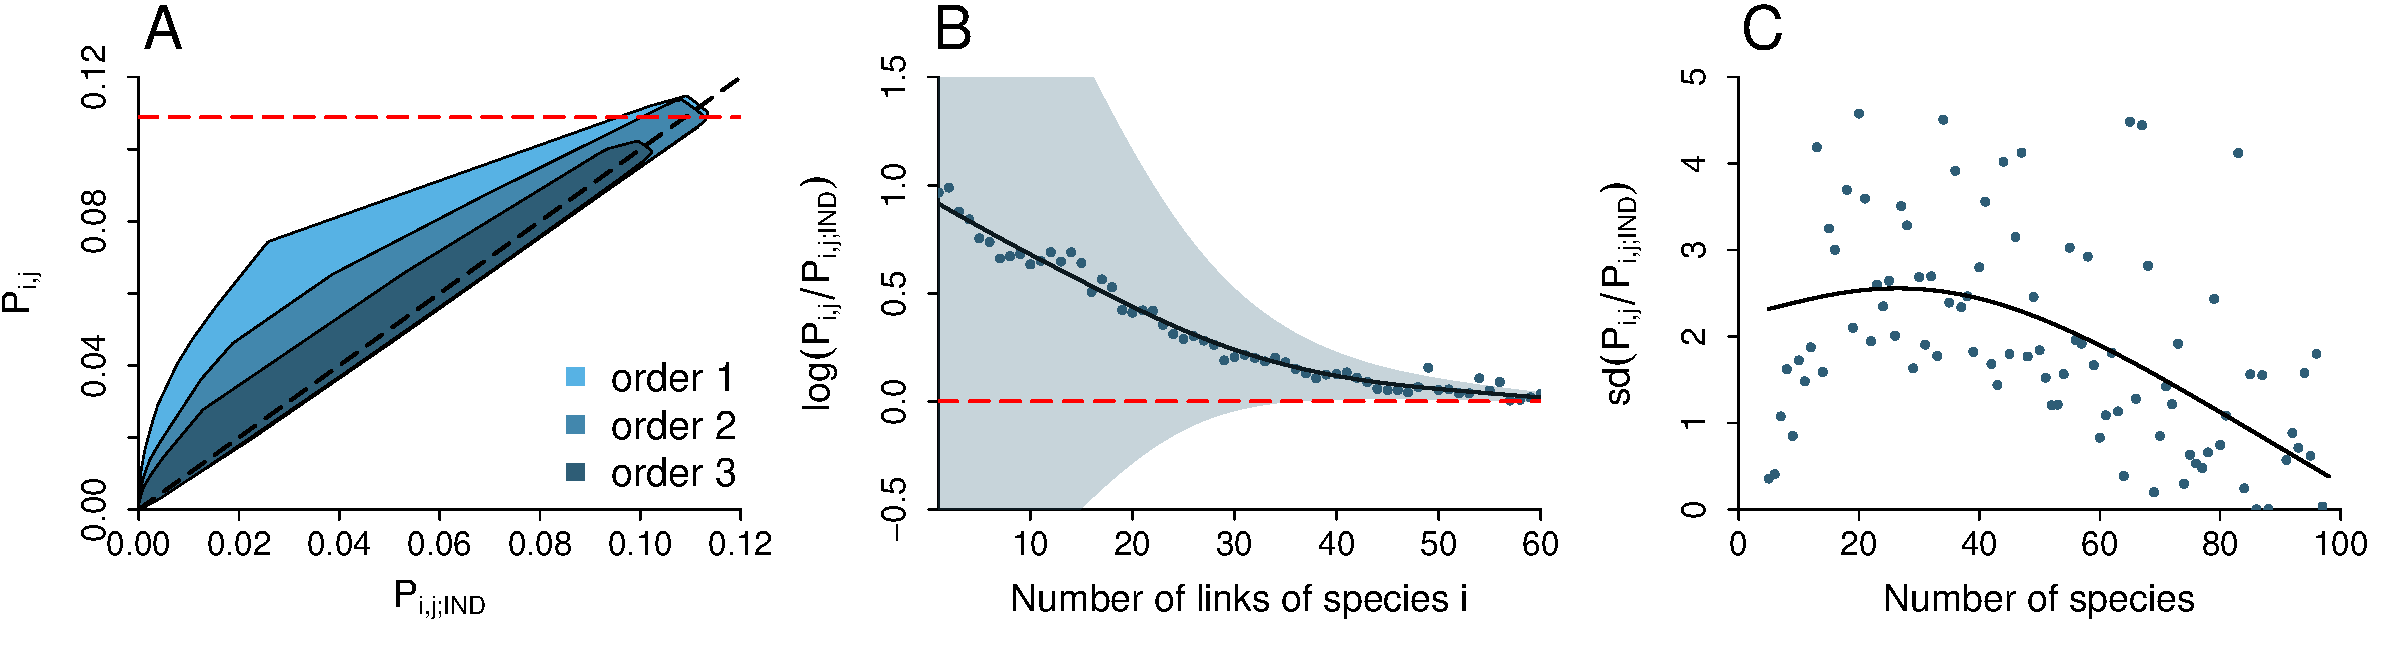
\includegraphics[width=\textwidth]{./chapitre2/fig1.eps}
\caption{Co-occurrence in multi-species networks.
(A) The disparity between observed co-occurrence ($P_{i,j}$) and independent co-occurrence ($P_{i,j;\text{IND}}$) decreases with the path length between nodes (species). The enveloppes are drawn around the 5\% and 95\% quantiles of all of the data, from 100 replicated simulations for every species richness value (5 to 100 species).
(B) The strength of co-occurrence ($log(P_{i,j}/P_{i,j;\text{IND}})$) decreases with the number of interactions of a species $i$ (\textit{i.e.} the degree of a node). Points represent the mean for a particular degree of node value (1 to 60). The solid line represents the overall trends and the grey envelopped refelcts the variance associated. At least 3000 values were used for each point.
(C) The standard deviation of the strength of association ($sd(P_{i,j}/P_{i,j;\text{IND}})$) and thus the variance decreases with species richness. Taken together, (B) and (C) imply that species distributions converge to independence with increasing species richness.}
\label{fig:1}
\end{figure}
%
\newpage
% Tables

%%-------
\begin{table}[h]
\centering
\begin{tabular}{r|r|r|r}
  Sites & Species 1 & Species 2 & Species3 \\
  \hline
1 & 0 & 1 & 1\\
2 & 0 & 1 & 1\\
3 & 1 & 1 & 0\\
4 & 1 & 0 & 1\\
5 & 0 & 0 & 0\\
6 & 1 & 1 & 1\\
7 & 0 & 1 & 0\\
8 & 1 & 0 & 0\\
9 & 1 & 0 & 0\\
10 & 1 & 1 & 0\\
  \end{tabular}
\caption{Presence/absence dataset for three species and 10 sites.}
\label{tab:2}
\end{table}
%%-------



%%-------
\begin{table}[h]
\centering
  \begin{tabular}{ll}
    \hline\noalign{\smallskip}
    General case & Linear chain \\
    \noalign{\smallskip}\hline\noalign{\smallskip}
    $\left(\begin{array}{ccc} p_{1|\overline{23}} & p_{1|2\overline{3}} & p_{1|\overline{2}3} \\ p_{2|1\overline{3}} & p_{2|\overline{1}\overline{3}} & p_{2|\overline{1}3} \\ p_{3|1\overline{2}} & p_{3|\overline{1}2} & p_{3|\overline{12}}\end{array}\right)$ &
    $\left(\begin{array}{ccc} p_{1|\overline{23}} & p_{1|2\overline{3}} & p_{1|\overline{23}} \\ p_{2|1\overline{3}} & 0 & 0 \\ 0 & 0 & 0 \end{array}\right)$
      \\
    \noalign{\smallskip}\hline
    \hline\noalign{\smallskip}
    Exploitative competition &  Apparent competition \\
    \noalign{\smallskip}\hline\noalign{\smallskip}
    $\left(\begin{array}{ccc} p_{1|\overline{23}} & p_{1|2\overline{3}} & p_{1|\overline{2}3} \\ p_{2|1\overline{3}} & 0 & 0 \\ p_{3|1\overline{2}} & 0 & 0 \end{array}\right)$  &
    $\left(\begin{array}{ccc} p_{1|\overline{23}} & p_{1|\overline{23}} & p_{1|\overline{2}3} \\ p_{2|\overline{1}\overline{3}}  & p_{2|\overline{1}\overline{3}} & p_{2|\overline{1}3} \\ p_{3|1\overline{2}} & p_{3|\overline{1}2} & 0 \end{array}\right)$
    \end{tabular}
  \caption{Direct associations between pairs of species for different modules. Entries indicate the fundamental conditional probabilities of occurence of species $i$ given the presence of species $j$ and the absence of species $k$. \emph{Linear chain}: 1 is the resource, 3 the top predator ; \emph{Exploitative competition}: 2 and 3 are the consumers; \emph{Apparent competition}: 1 and 2 are the resources. When $p_{i|j\overline{k}}=0$, it means that species $i$ cannot be found without $k$. When two species $i$ and $j$ do not interact directly, if the absence of species $k$ do not impact species $i$ survival then : $p_{i|j\overline{k}}$=$p_{i|\overline{jk}}$. For apparent competition, if species 1 and 2 are interchangeable for species 3 then : $p_{3|1\overline{2}} = p_{3|\overline{1}2}$.}
  \label{tab:1}
\end{table}
%%-------


%

\chapter{HOW ECOLOGICAL INTERACTIONS CAN AFFECT BIODIVERSITY FORECAST}

Le chapitre est en cours de développement. L'avancement est indiqué dans le rapport du troisième compte-rendu de comité de thèse.

\chapter{Vers une théorie métabolique de la biogéographie}
\label{chap4}


\subsection{Résumé en français du troisième article}

Dans ce chapitre, je présente une formulation énergétique du modèle
de la TTIB \citep{Gravel2011}. Pour cela, je transforme les îles en
quantités de producteurs primaires. À partir de cette quantité,
les espèces des niveaux trophiques supérieurs peuvent coloniser l'île.
Ces espèces sont liées les unes aux autres par des relations trophiques.
Le réseau est décrit pour l'ensemble des interaction à l'échelle régional,
il s'agit d'un metaweb. Les espèces peuvent coloniser îles tant que toutes les
espèces peuvent maintenir une population minimal local sur l'île.
Je propose un calcul simple mais astucieux pour intégrer les différences
de consommations entre les différents niveaux trophiques. Le calcul est
basé sur la biomasse des espèces mais aussi sur le transfert énergétique,
qui représente la quantité d'énergie qui passe d'un réseau à l'autre.
Lorsqu'une espèce arrive sur l'île mais que l'ensemble des espèces ne peuvent
plus toutes soutenir une population minimale localement, alors un processus
d'extinction est enclenché. À partir de cette nouvelle formulation de la
TTIB, j'obtiens une relation espèce-énergie (SER) pour laquelle la probabilité
d'occurrence des les espèces en fonction de leur masse corporelle et
leur statut trophique est connu. Je montre alors l'importance du statut trophique
pour comprendre la probabilité d'occurrence et montre alors comment une relation
energie-longeur de la chaine trophique se met en place.

Cette approche est un pas significative vers une intégration plus aboutie des
mécanismes écologiques dans la TIB, notamment pour les
interactions biotiques. Je prolonge le travail de la TTIB et
je fais un premier rapprochement avec la théorie métabolique de l'écologie.
Bien que le modèle proposé soit relativement simple, il est une pierre solide pour
aller plus loin dans la théorie. De plus, au regard de l'abondante littérature
relative aux relations allométriques, il me semble essentiel de comprendre
comment les contraintes énergétiques, exercées à l'échelle de l'individu,
se propagent à l’échelle des populations puis aux échelles biogéographiques.



\subsection{Publication envisagée}

Présentement, l'article offre des perspectives intéressantes sur une
théorie métabolique en biogéographie mais aussi des pistes de réflexion
 pour s'affranchir simplement de certaines contraintes de modélisation
qui pourraient hautement  complexifier le modèles (par exemple,  je ne considère
pas explicitement de dynamiques de population). Je vois deux opportunités
associées au présent travail. Premièrement, orienter davantage mon travail
sur les aspects techniques et mathématiques du modèle et essayer,
par exemple, de dériver une solution approchée du modèle.
Cela m'orienterait vers une publication plus technique
pour un journal plus spécialisé. Deuxièmement, aller plus loin dans l'exploration
des possibilités offertes par le modèle, insister sur les perspectives, notamment
sur l'impact de la structure sur la relation énergie -espèces. Cela m'orienterait plutôt vers
un article de perspective pour un journal d’écologie plus généraliste.


Pour cet article ma réflexion a été alimentée par discussion avec Dominique Gravel,
Miguel Araújo, Loïc Pelissier que je remercie. Je me suis occupé de concevoir le modèle,
d'implémenter le modèle et de sortir les résultats et de l'analyser.
J'ai écrit la première version du modèle et j'ai bénéficié d'apport significatif
de Dominique Gravel qui a fait une relecture complète du manuscrit. Je remercie
également chaleureusement Kevin Solarik qui m'a apporté de nombreuses
relectures mais aussi des suggestions pertinentes.
Cet article est également la base de réflexion du travail que
j’aimerais mener dans un projet post-doctoral.


\subsection{Résumé de l'article en anglais}



\emph{Les sections qui suivent sont celles de l'article publié.}
\section{Title}\label{title}

Towards a metabolic theory of island biogeography

\section{Abstract}\label{abstract}

Energy availability shapes biodiversity: solar radiation and water
availabilities well describe terrestrial ecosystems as well as sea
surface temperature and nutrients availability describe maritime ones.
Energy has been early envisioned as a key factor to understand
biodiversity over large latitudinal gradients. At the community scale,
food webs structure the partitioning of energy from the primary
producers to the top predators. Despite its crucial importance, energy
has been overlooked in classical theories of biogeography that either
assume ecological equivalence (\emph{e.g} the Theory of Island
Biogeography) or remain focused on the concept of the ecological niche.
To rectify this, we develop a theory of biodiversity distribution based
on first principles of energetic constraints, including allometric
relationship, in order to investigate the impact of trophic interactions
along an energy gradient. Based on this theory we derive expected
species richness and network structure along gradients of primary
productivity. Our model offers immense possibilities for the integration
of community ecology with biogeography as well as insights to propose
better species distribution models.

\section{Introduction}\label{introduction}

Disentangling the relative contribution of the different processes
shaping biodiversity distribution is the central objective of
biogeography. While biogeographers clearly envision the list of
ingredients needed to understand species distribution
\citep{Thuiller2013}, they miss the framework to mix them in the right
amount and to investigate the biogeography of ecological communities. We
will likely fail to predict accurately biodiversity responses to global
changes as we keep our focus strictly on abiotic factors \emph{i.e}
temperature and precipitation, while continuing to overlook biotic
interactions \citep{Wiens2011} and short-term evolutionary responses
\citep{Lavergne2010}. At the core of this issue is the need for an
integrated approach at the crossroad between species distribution
modelling and community ecology.

Biotic interactions should be integrated as a constraint for species
co-distribution in meta-communities \citep{Jabot2012, Cazelles2016a}.
Ecological interactions may explain, at least partially, the dynamics of
local extinctions, which in turn would further explain some properties
of the geometrical shape of species ranges \citep[\emph{e.g.} nested
distributions of parasitoid and its host,][]{Shenbrot2007}. We have
however limited evidence of the effect of biotic interactions on large
scale species distribution \citep[see Chapter \ref{chap3} - but
see][]{Gotelli2010}. Incidentally, two of the most influential models in
biogeography assume ecological equivalence of species; the Theory of
Island Biogeography of MacArthur and Wilson \citep[hereafter
TIB,][]{MacArthur1967} overlook the variation among species
characteristics and ignore their arrangement in organized ecological
networks. In his neutral theory, Hubbell assumes that individuals of
different species are ecologically equivalent and predicts the
distribution of abundance without considering interactions
\citep{Hubbell1997, Hubbell2001}. These two theoretical models have been
proven relevant for certain groups of species and inadequate for others,
and none of them were initially intended to describe exhaustively the
structure of ecological communities. The integration of ecological
interactions into biogeography however offers promising perspectives and
a much extended range of predictions \citep{Holt2010, Gravel2011}.

The TIB is well-suited to explore the consequences of ecological
interactions on community structure at broad spatial scales, as it
includes two fundamental processes of biogeography, immigration and
extinction, in an elegant fashion that eases its extension
\citep{Losos2010, Warren2015}. Building upon the classical model of
MacArthur and Wilson, recent studies have included various forms of
interactions in the TIB \citep{Gravel2011, Cazelles2016a}. The regional
species pool becomes a \emph{metaweb}, not only listing potential
colonists but also their interactions. With this approach, species are
inter-dependent entities with specificities (\emph{e.g.} a given trophic
level) rather than indistinguishable units. As a consequence,
colonization and extinction rates vary with respect to species identity
\emph{and} the composition of the local community. \citet{Gravel2011}
proposed the Trophic TIB (hereinafter TTIB) to represent food web
assembly on isolated communities, where predators can persist locally as
long as they find at least one preys. More generally,
\citet{Cazelles2016a} presented a Lotka-Volterra like model in which the
composition of the local community determines both colonization and
extinction rates. Adding new ecological processes in the TIB increases
realism, at the cost however of reducing its simplicity. It provides an
extended list of predictions, which have yet to be proven significantly
better than the original theory \citep[see][]{Cirtwill2015}. Extending
the TIB while preserving its elegance is a challenging and technical
issue. Here we propose to reformulate the TTIB in terms of energetic
constraints in attempt to solve this challenge.

The TIB was originally meant to predict and explain the common
observation of increasing species richness with island area. Another
ubiquitous and fundamental observation in biogeography is the
latitudinal diversity gradient
\citep[LDG,][]{Rhode1992, Stevens1989, Evans2005}. The productivity of
primary producers is generally found the best predictor of species
richness at large spatial scales \citep{Evans2005, Storch2005}. Others
found a strong correlation between richness, water availability and
temperature \citep{Currie1993, Hawkins2003}. Several mechanisms have
been proposed to explain this relationship \citep[see][ for a
review]{Currie2004, Evans2005}, including higher speciation rates in
tropical areas, greater biomass and finer niche partitioning. Recently,
some authors investigated how networks could change with latitude. Based
on the meta-analysis of 196 empirical food webs, \citet{Cirtwill2015a}
shown that ecological networks of interactions also vary along this
gradient but that the density of links remains constant throughout. In
the majority of ecosystems theses authors studied, an increased energy
results in a wider niche space, rather than an increase of niche breadth
poleward. Similarly, \citet{Albouy2016} reconstructed marine networks
across the globe and found significant latitudinal-network gradients
(LNG). These studies are however descriptive only, as there is currently
no theory to explain how and why energy constraints should impact food
web structure. In 1983, \citet{Wright1983} developed the species-energy
theory and replaced the ``area'' with ``available energy'' to derive a
meaningful Species Energy Relationship (SER). Although area and energy
may bring more information taken together \citep{Storch2005}, the
rationale behind it allows the derivation of species abundance and
occurrence probability based on energetic constraint \citep{Wright1983}.
Wright's approach however do not specifically account for network
structure and thereby remains limited to species richness.

Species do not escape from the laws of thermodynamics and as a
consequence, despite the complexity of evolutionary trajectories, many
key ecological properties and processes scale with body mass
\citep[\emph{i.e.} metabolic theory of
ecology][]{Brown2004, Woodward2005a}. The scaling of the metabolic rates
with body mass is the fundamental observation underlying this theory
\citep{Gillooly2001}, which typically follows a power function with
coefficients often between 2/3 and 3/4 \citep{White2013}. Even if all
the relationships are not well-understood \citep[see the case of
abundances reviewed in][ and the recent relationship between prey and
predator biomasses \citet{Hatton2015}]{White2007}, the ubiquity of
allometric relationships makes body mass distribution a key variable to
reduce the complexity of ecosystems. Allometric relationships and energy
flows also provide the mean to parameterize models of population
dynamics \citep{Yodzis1992}. Recent developments of food web theory have
convincingly shown that allometric relationships are the cog to analyze
the properties of ecological networks \citep{Gravel2013, Petchey2008},
their dynamics \citep{Brose2006} and to characterize the role of species
within them \citep{Schneider2012}.

Our objective in this study is to develop a theory of biodiversity
distribution based on first principles of energetic constraints in order
to investigate the impact of trophic interactions on the
latitudinal-diversity gradient. We propose to extend the model of the
TTIB following the vision of \citet{Wright1983}. As a consequence, our
theory encompasses both the species-area and the species-energy
relationships, making it a very general framework to understand and
predict biodiversity distribution. In addition, the explicit integration
of trophic interactions allows the development of a vast array of
testable and insightful predictions, including the expected
latitudinal-network gradient. To do so, we propose a theoretical model
of food web assembly driven by colonization from the regional metaweb
and energetic constraints. We derive expected species richness and
network structure along gradients of primary productivity. We use
``Lindeman'' \citep{Lindeman1942} transfer efficiency (\emph{i.e.}
energy transferred to another trophic level) to integrate
species-specific differences in their source of energy. We derive a SER
and the relationship between body-mass distribution and available
energy. Our model formalizes the initial hypothesis of Lindeman and
offers immense possibilities for the integration of community ecology
with biogeography.

\section{Model description}\label{model-description}

The model developed by MacArthur and Wilson predicts species richness on
an island according to the size of the island and its distance from the
mainland \citep{MacArthur1967}. One promising direction to extend this
theory is to include biotic interactions into the classical model
\citep{Holt2010, Gravel2011, Cazelles2016a}. Following this avenue, we
consider explicit interactions among the regional pool of species based
on allometric relationships. Body mass is used to determine the quantity
of energy a given species requires to maintain its local population on
an island. Extinction follows if the island cannot sustain a minimal
population of any given species. Therefore, in the model described
below, we simulate the TIB with purely stochastic colonization events
together with deterministic extinction based on an energy rational.

We consider an island as an isolated piece of land covered by a maximal
quantity of primary producers, which determine the amount of available
energy upon which a food web can develop. We denote \(E_0\) the maximal
amount of energy available for herbivores and consider it to vary
proportionally to island area. Here we do not enter the specificities of
how productivity scales with area, as in some situation it could scale
linearly or not {[}\emph{e.g.} for lakes when the volume determines
productivity \citep{Post2000}. As a consequence, the model explains both
the scaling of richness with island area and productivity, with the same
underlying principle that a minimal population size is required for
persistence. We make two additional simplifications: the diversity of
primary producers is not taken into account, and the production is
constant over the time.

The regional pool of species in the TIB is the number of species \(P\)
and the tropic interactions among them. Following \citet{Cazelles2016a},
potential interactions among them are determined using the niche model
\citep{Williams2000}. We furthermore assume the niche axis to be the
body size of the species \citep{Gravel2013} and that species which are
without any links in the metaweb are determined to be herbivores. Note
that primary producers are not included in the niche model but the
source of energy of herbivores. They are rather included in the total
energy \(E_0\) (see below) consumed by herbivores. As a consequence,
trophic level is strongly correlated to body mass, with herbivores often
the smallest and top predators the largest. Although this assumption is
an oversimplification of the determinants of ecological interactions, it
remains reasonable for marine ecosystems \citep{Trebilco2013}, where
allometric relationships have been used to infer food web structure
\citep{Gravel2013}.

Following \citet{Gravel2011}, we assume that the colonization of
herbivores/predators is successful only if they find at least one of
their habitat/prey on the given island. Additionally, we propose that
colonization events are possible only if the energetic requirements to
maintain local populations exceeds the primary production. In this case,
energetic constraints and network topology determine the identity of
species to go extinct. Colonization events are assumed to be purely
stochastic, while extinctions are deterministic, control by the
energetic constraints \citep[this difference in stochastic nature
between these fundamental processes of biogeography has been recently
supported in][ where the authors show that extinction probability
decreases with the presence of resource/prey on the
island]{Cirtwill2015}.

\subsection{Energetic constraints on local food
webs}\label{energetic-constraints-on-local-food-webs}

The rational for energetic constraints is simple: local populations need
a certain amount of energy to maintain a minimum level of activity
otherwise they die from starvation. Under this constraint, species
richness locally increases until the energy available on the island
(\(E_0\)) is no longer sufficient for all populations because of
inefficient energy transfer at each trophic interactions. Therefore all
population on the island are maintained as long as the inequality below
holds true:

\begin{equation} \sum_i e_i \leq E_0\label{eq:chp4id0}\end{equation}

where \(e_i\) is the energy uptake of the insular population of species
\(i\). We now need to define a rule to set the the minimal energy a
population needs to survive on the island. For a given species \(i\),
energy requirements of any individual is derived from allometric
relationships proposed by the metabolic theory of ecology
\citep{Brown2004}, of the form \(c_im_i^b\) where \(c_i\) is a constant,
specific constant, \(m_i\) the body mass of species \(i\) and \(b\) the
coefficient of power \citep[between 2/3 and 3/4][]{White2013}. We do not
integrate intraspecific variability in body mass and thus \(m_i\) is a
constant for a species. The energy uptake associated to a minimal viable
population (hereafter MVP) of \(n_i\) individuals becomes \(n_im_i^b\).
\citet{Shaffer1981} defined the MVP as ``\emph{{[}\ldots{}{]} the
smallest isolated population having a 99\% chance of remaining extant
for 1000 years despite the foreseeable effects of demographic,
environmental and genetic stochasticity, and natural catastrophe}'',
highlighting that the smallest portion of a population has the highest
possible extinction risk (extrapolated as time to extinction). The key
problem is wether or not the MVP is size dependent. The most
conservative assumption is to consider it to be a constant.
\citet{Lande1993} however shown that the time to extinction is affected
by the mean population growth rate, which underlies that species
characteristics may lead to a heterogeneity in MVP. Moreover,
\citet{Savage2004} had developed a framework within which they proved
the growth rate to be proportional to \(m_i^{-b}\). Based on these
results, we explore two different rules for extinctions: (1) MVP is
equal for all species: \(n_i=n_0\), and (2) MVP scales with the growth
rate \(n_i=n_0m_i^{-b}\). For both scenarios, species \(i\) can survive
only if the energy expenditures can be covered, \emph{i.e} if the energy
available is greater than: \(n_ic_im_i^b\).

\subsection{Energy fluxes and transfer
efficiency}\label{energy-fluxes-and-transfer-efficiency}

Although the expression of energy consumption is similar among species,
they obtain it from different sources: herbivores feed on primary
producers, whereas predators feed on a set number of secondary
consumers. The primary production must therefore be tracked as it moves
up through the food chain. To deal with this, we propose to convert the
energy costs for maintaining predator populations into additional
populations of herbivores to be maintained. To exemplify this idea, we
start with the simplest trophic network where a predator \(j\) feeds
upon a herbivore \(i\). The cost to maintain the MVP of \(i\) is
\(n_ic_im_i^b\) and \(n_jc_jm_j^b\) for \(j\). For the latter, we
convert \(n_j\) into an extra population of \(i\), \(n_{i,j}\) herbivore
individuals dedicated to \(j\) consumption. Furthermore, we account for
the energy loss during consumption by including a transfer efficiency
\citep[sensu][]{Lindeman1942} \(\tau\). Hence, the conversion from
\(n_{j}\) to \(n_{i,j}\) is given by the following equation:

\begin{equation} \tau n_{i,j} c_im_i^b = n_jc_jm_j^b \label{eq:chp4id1}\end{equation}

the energy requirements of \(n_j\) are converted into a energy expressed
in term of a population of \(i\) based on which we obtain the population
size of \(i\) needed to maintain a MVP of \(j\):

\begin{equation} n_{i,j} = \frac{n_jc_j}{\tau c_i} \left( \frac{m_j}{m_i} \right)^b \label{eq:chp4id2}\end{equation}

We postulate that the transfer efficiency is constant across trophic
levels, which is likely an oversimplification of the reality as
suggested by the sparse empirical data available
\citep{Trebilco2013, Brown2003}. We now add a new predator \(k\) feeding
on \(j\) (the predator of \(i\)) to the insular food web. According to
our reasoning, we must covert \(n_k\) into \(n_{i,k}\). To do so, we
start by converting \(n_k\) into a population of \(j\):

\begin{equation} n_{j,k} = \frac{n_kc_k}{\tau c_j} \left( \frac{m_k}{m_j} \right)^b \label{eq:chp4id2}\end{equation}

We now turn \(n_{j,k}\) into a herbivore population:

\begin{equation} n_{i,k} = \frac{\frac{n_kc_k}{\tau c_j} \left( \frac{m_k}{m_j} \right)^bc_j}{\tau c_i} \left( \frac{m_j}{m_i} \right)^b \label{eq:chp4id3}\end{equation}

which gives:

\begin{equation} n_{i,k} = \frac{n_kc_k}{\tau^2 c_i} \left( \frac{m_k}{m_i} \right)^b \label{eq:chp4id3b}\end{equation}

In a similar fashion, for a linear trophic chain, we can demonstrate
that the additional population of herbivore \(i\) necessary to maintain
predator \(j\) of level \(l\) is:

\begin{equation} n_{i,k} = \frac{n_jc_j}{\tau^l c_i} \left( \frac{m_j}{m_i} \right)^b \label{eq:chp4id4}\end{equation}

In many cases, a predator feeds on an array of prey species rather than
a single one. As such, it uptakes its energy from the different sources
and we must account for all of them. We assume that energy costs
associated with maintaining the local predator are minimal. Therefore,
\(n_j\) is converted into \(i\), the herbivore linked to \(j\) for which
(\ref{eq:chp4id4}) is minimal. Basically, \(i\) should be a large and
separated from \(j\) by a low number of species. Hence, on the island,
the species richness increases as long as the inequality below holds
true:

\begin{equation} \sum_i c_in_im_i^b + \sum_j \frac{n_jc_j}{\tau^{l_j} c_i} \left( \frac{m_j}{m_{i_j}} \right)^b \leq E_0 \label{eq:chp4id5}\end{equation}

The first term is the energy cost for maintaining populations of
herbivores, the second term is associated to higher trophic levels:
predator \(j\) is converted into herbivore \(i_j\) from which it is
separated by \(l_j\) links. For the sake of simplicity, we make an extra
assumptions: \(c_i\) values are constant among species and set to 1.
Therefore, if we assume that MVP is constant (scenario 1), inequality
\ref{eq:chp4id5} becomes:

\begin{equation} \sum_i m_i^b + \sum_j \frac{1}{\tau^{l_j}} \left( \frac{m_j}{m_{i_j}} \right)^b \leq \frac{E_0}{n_0} \label{eq:chp4id5a}\end{equation}

Similarly, if we assume \(n_i=n_0m_i^{-b}\) and \(n_j=n_0m_j^{-b}\)
(scenario 2), then:

\begin{equation} \sum_i 1 + \sum_j \frac{1}{\tau^{l_j}} \left( \frac{1}{m_{i_j}} \right)^b \leq \frac{E_0}{n_0} \label{eq:chp4id5b}\end{equation}

The left side of this equation provides the minimal energy needed to
sustain all populations while the right side is the total amount of
energy available. Therefore, the maximal population of species \(i\)
without any extinction is given by converting the extra amount of energy
available into an additional population of species \(i\), the population
of \(i\) we get is denote \(n_{i,max}\). The range \([n_i, n_{i, max}]\)
is then the range of possible fluctuations of species \(i\) without any
new extinction event.

\subsection{Extinctions}\label{extinctions}

When the local primary production cannot sustain the establishment of a
new immigrant, \emph{i.e.} when inequality \ref{eq:chp4id5} is no longer
verified, its arrival is either impossible or lead to extinction of
other species. In the latter situation, we must determine the identity
of species that will go extinct, which remains a significant challenge
that will not be undertaken here given its complexity highlighted by
recent theoretical studies \citep{Saterberg2013, Zhao2016}. To overcome
this concern, we use two scenarios: (1) \emph{random extinction}: any
species can go extinct, and (2) \emph{costs-based extinctions}: the
probability of extinction is proportional to the energetic costs of the
species. Once an extinction occurs, we ensure that all species remain
linked to at least one herbivore, otherwise unlinked species will too go
extinct. Finally, extinctions are set to occur until \ref{eq:chp4id5} is
satisfied. Note that the deterministic nature of extinctions lays in in
the fact that they occur when energy is lacking, the identity of the
species that actually goes extinct remains stochastic.

\begin{longtable}[]{@{}lll@{}}
\caption{Hypotheses associated to the four scenarios.
\label{tbl:scena}}\tabularnewline
\toprule
Scenario & MVP & extinction\tabularnewline
\midrule
\endfirsthead
\toprule
Scenario & MVP & extinction\tabularnewline
\midrule
\endhead
A & \(n_0\) & random\tabularnewline
B & \(n_0\) & costs-based\tabularnewline
C & \(n_0m^{-.75}\) & random\tabularnewline
D & \(n_0m^{-.75}\) & costs-based\tabularnewline
\bottomrule
\end{longtable}

Although the assumptions we have made here are likely unrealistic, our
intentions are merely to examine the model under the special case of an
optimal energy allocation on an island. These assumptions remain
acceptable as long as we focus on the qualitative consequences in term
of community dynamics. As an important remark, the energy cost
associated to one predator is not based on inherent properties only, as
it is determined also by the identity of its preys present on the island
(in other words, via apparent competition). Hypotheses made for the four
scenario are recapitulated in Table \ref{tbl:scena}.

\subsection{Simulations}\label{simulations}

Every simulation starts with the generation of the regional metaweb of
100 species. To do so, we first draw a number \(p_i\) for all species
from a uniform distribution from the range {[}0,3{]}. Numbers \(p_i\)
are then sorted, the lowest values are assigned to the herbivores and we
use the vector obtained as the niche axis in the niche model, with
connectance set to \(0.05\) \citep{Williams2000}. Species that are not
connected are assumed to be herbivores and to allow comparisons among
simulation we standardize the number of herbivore to 10. To do so we
keep generating new metawebs until one we obtain one metweb with 10
species that were not connected. We also use the \(p_i\) number to
derive the biomass of all species, we do so by using \(10^{p_i}\). The
smallest species has the smallest niche axis.

We simulated the model along a gradient of energy ranging in
\(\frac{E_0}{n_0}\) from \(.1\) to \(10^8\). We start with an empty
island and at any time step, any species of the metaweb has a
probability \(c=0.001\) of colonizing the island. If a successful
colonization occurs if available energy on the island allow to sustaint
a MVP of the new species. For all time step we record the species on the
island. We perform 125,000 iterations and discard 25,000 burn-in
iterations and the 100,000 remaining to do our analyses. For all the 91
values of the energy gradient we used 100 replicates, meaning 100
different regional metawebs.

\section{Results}\label{results}

We found a sigmoidal SER for all scenarios (Fig. \ref{fig:etib1} A).
Under scenario A, for instance, species richness increased exponentially
with the increase in energy, where more species were allowed to colonize
the island (Fig. \ref{fig:etib1}). SER reached saturation much faster
under scenarios C and D than under the scenarios A and B, due to the
difference in energy uptake. Under scenarios C and D the MVP decreased
with body mass, which allows higher species richness or a comparable
amount of energy. Remarkably, species richness was smaller for scenarios
where the extinction rate was cost-based than randomly based (Fig.
\ref{fig:etib1} A-B), which also results in less variability (Fig.
\ref{fig:etib1} C).

Occurrence probability increases with available energy and decreases
with trophic level for all scenarios (\ref{fig:etib2}). Herbivores were
found to colonize the island first, followed by predators of increasing
trophic level. The trend was similar for all scenarios, and more
pronounced for those where extinction is cost-based (scenarios B and D).
When species occurrence probabilities were grouped by body mass, only
significant differences were found within scenario B (\ref{fig:etib3}).
Taken together, these results highlight the importance of network
structure. Here, we outline the importance of colonization, where the
shortest path between herbivore and predator is extremely important
especially given it strongly impacts the cost of a species; suggesting
that this is the cause of the main differences among random and
cost-based extinction rates.

The average species body mass increased with energy under scenarios A
and B, but decreased under scenarios C and D. The reduction of MVP with
body mass would therefore allow for larger species to maintain on small
island (\ref{fig:etib4} A-D). We see a similar trend for the number of
prey species, which increases with energy in scenarios A and B, while it
decreases in scenarios C and D (\ref{fig:etib4} E-H). Ultimately,
generalist species have a much higher rate of successful colonization
under low energy in scenarios C and D. When the MVP is smaller, larger
species can colonize and their probability of success is higher as they
have more preys in average \citep[due to the use of the niche model and
body mass as the niche axis][]{Williams2000, Gravel2013}. Finally, under
scenarios A and B small species with several predators colonize low
energy islands while under scenarios C and D the same species colonize
the island with higher energy availability as they are preceded by
larger and more generalist species (\ref{fig:etib4} I-L).

\section{Discussion}\label{discussion}

We proposed a of the classical TIB in terms of energy and turns the
well-known colonization/extinction dynamics into a successional assembly
process, starting with herbivores and then building up the food web. We
link species extinction to energy requirements, making extinctions more
mechanistic than in the TIB. Moreover, species are no longer
ecologically equivalent as in TIB \citep{Lomolino2009}, they have a body
mass, a trophic level and specific interactions. Based on these
characteristics, we compute a cost associated to the MVP on the island.
Therefore an insular community become an assemblage of population that
should not exceed a given amount of energy. Although the energy
allocation we use here is simple, we think it is a significative step
towards the interactions of community dynamics in biogeography theory.
The next step would be to integrate more realistic energy partitioning
\citep{DeRuiter1995} and to take into account variations of population
caused by bottom up and top-down effects we introduced here
\citep{Terborgh2001, Brown2013}. Ultimately, the downscaling from
species to population we attempted here should lead to integrate
principles of population dynamics as well as concepts of the community
ecology such as the stability of a community \citep{Allesina2012a}. This
would lead us to follow the path MacArthur and Wilson mapped 50 years
ago: ``{[}\ldots{}{]} biogeography appears to us to have developed to
the extent that it can be reformulated in the terms of the first
principles of population ecology and genetics?''
\citep[p.183]{MacArthur1967}.

The formulation of the TIB in terms of energy offers a great hope
towards a mechanistic biogeography as it strongly eases the integration
of ecological processes. As an example, we here showed how three
ecological necessities, overlooked in classical theories, can be taken
into account: 1- the necessity of a minimal population to sustain on
island 2- the necessity of finding resources/preys to maintain this
population and 3- the difference of energy uptake due to variations in
body mass and trophic levels among species. Based on this integration,
we showed how the structure of the community is constrained by the
energy availability on islands. We also pointed out that the structure
of the food webs, which determines the energy requirements of the whole
community, controls the species richness and the characteristics of
species present of the island. In our study, we study the SER under two
scenario regarding the MVP: either it decreased with the body mass or
not. The results were qualitatively similar but quantitatively
different: in the first case, larger species can colonize earlier which
increases the species richness of the island. Having a lower MVP for
larger species could compensate the energy cost associated to the
maintenance of a larger body. Furthermore, this could explain the
``energetic equivalence rules'' \citep{Nee1991} which states that
species have an equal share of energy allocated irrespective to their
body mass \citep{Brown2003, Damuth2007}. In our case, this holds true as
long as the island is ``saturated'' by species. Remarkably, under this
condition, the relationship between the logarithm of the species
richness and the logarithm of available energy (\ref{fig:etib1} B) is
linear, which is consistent with empirical observations (see Fig 3. and
Fig 4. in \citet{Wright1983}). Over evolutionary scales, these
observation, would also be consistent with the Ecological Limits
hypothesis to diversification dynamics \citep{Rabosky2015}.

Our findings suggest the existence of a clear relationship between the
trophic status of species and its occurrence probability: species of
higher trophic levels, irrespective of their body mass, colonize island
with higher energy. This indicates that the food-chain length is limited
by the energy availability. Remarkably, a comparable relationship has
already been observed by \citet{Post2000}, who have found a correlation
among maximal food-chain length and lake size which is consistent with
the idea that higher predator needs larger areas to a sufficient amount
pf prey to survive in the lakes. This would suggest that larger
predators actually uses a broader areas to find more energy.

Using our framework, we showed that under scenarios C and D (for which
MVP decreases with the body mass), generalist species are the first to
colonize the island. Remarkably, the early colonization of generalist
species has been highlighted by \citet{Piechnik2008} when they revisited
the classical study by \citet{Simberloff1969}. Also, reading Fig
\ref{fig:etib4} G-H in the direction of a loss of energy we observe an
increasing in generalist species such as currently observed
\citet{Clavel2011}. The classical TIB has provided a theoretical basis
for the SAR \citep{MacArthur1967}, that has been largely used in
conservation to determine the size of protected areas
\citep{Neigel2003}. However, as in the TIB, the SAR ignores the identity
of species, there is currently no theory integrating the position of a
species within the network it is embedded to predict its distribution.
However, the role of a species in the network must be of first
importance to understand the consequence of its loss
\citep{Saterberg2013}. The model we described here offers testable
hypothesis regarding the role of the species that are expected to go
extinct first: from the higher trophic level to the lower and from the
more generalist to the lower.

Finally, our framework is an opportunity to review the way we build
SMDMs. Here, our model describes the food web dynamic associated to
patch of primary producers. Fortunately, the primary production have
been proven highly correlated to climate variables
\citep{Wright1983, Hawkins2003, Evans2005} and are readily quantifiable
using index such as the normalized difference vegetation index
\citep[NDVI][]{Evans2005}. According to our framework, such quantity is
not only a proxy to assess the diversity of primary producers and the
productivity associated but also a potential metric of the species
richness \citep{Wright1983} and even a predictor of the structure of the
network (a predictor of the food chain length for instance). Current
species distribution model are based on the correlation between abiotic
factor and its occurrence probability is ascribed to this abiotic niche
while its presence could be best explained by the presence of its prey
(see chapter \ref{chap4}). Therefore, focusing on the prediction of the
distribution of primary producers while using information about energy
they should provide to add higher trophic levels based appears, in the
light of our study, as a promosing avenue to propose new approach that
would likely enhance the robustness of the scenarios of tomorrow's
biodiversity.

\begin{figure}[htbp]
\centering
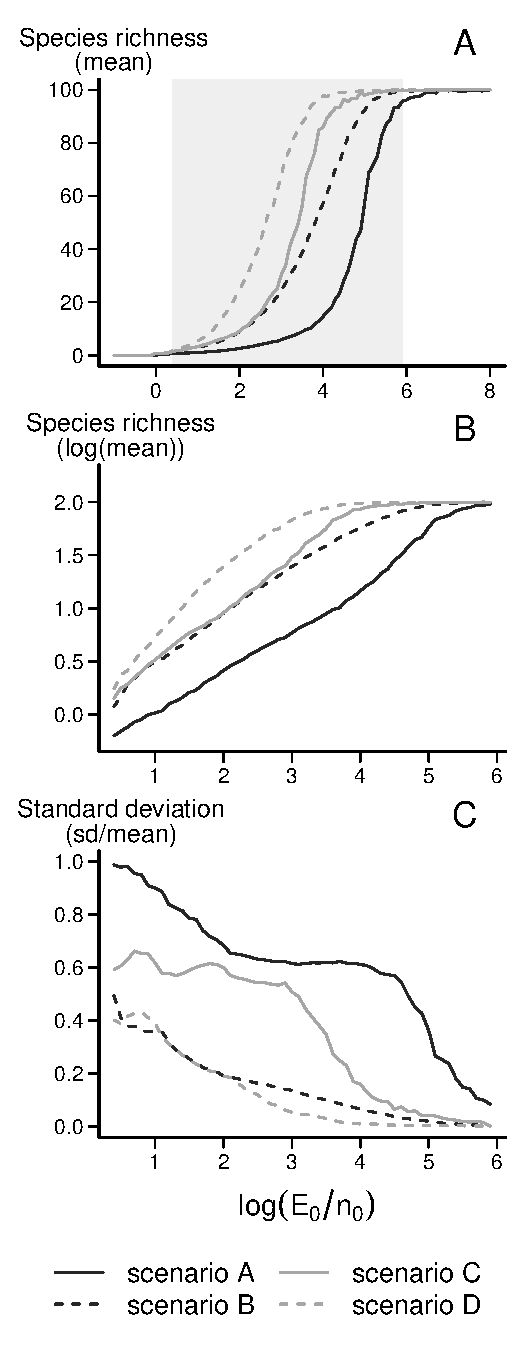
\includegraphics{chapitre4/fig/fig1.pdf}
\caption{\textbf{Species-Energy Relationship} using 100 replicates for
each of the four scenarios for (A) mean species richness, (B) logarithm
of the mean, and (C) coefficient of variation.\label{fig:etib1}}
\end{figure}

\begin{figure}[htbp]
\centering
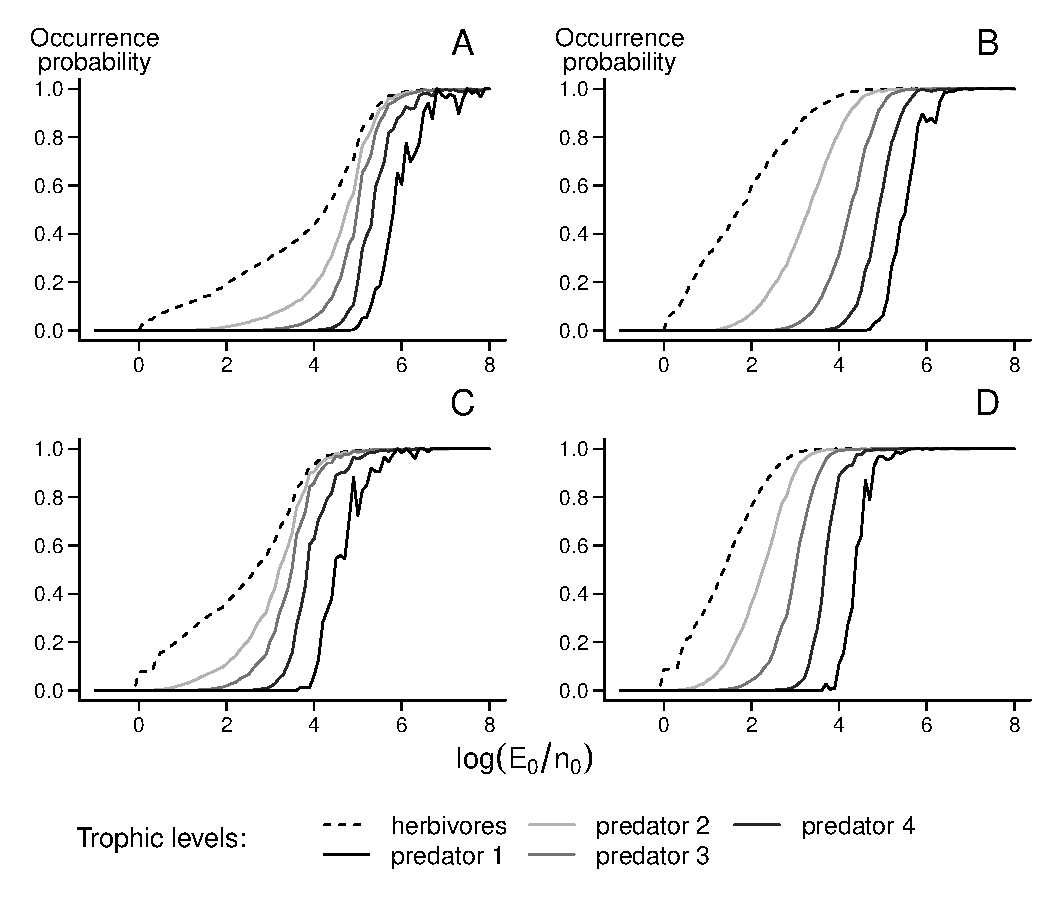
\includegraphics{chapitre4/fig/fig2.pdf}
\caption{\textbf{Species occurrence probability along an energy
gradient, grouped by trophic level}; herbivores, or by their shortest
path linking to a herbivore species. The top right letters indicates the
scenarios.\label{fig:etib2}}
\end{figure}

\begin{figure}[htbp]
\centering
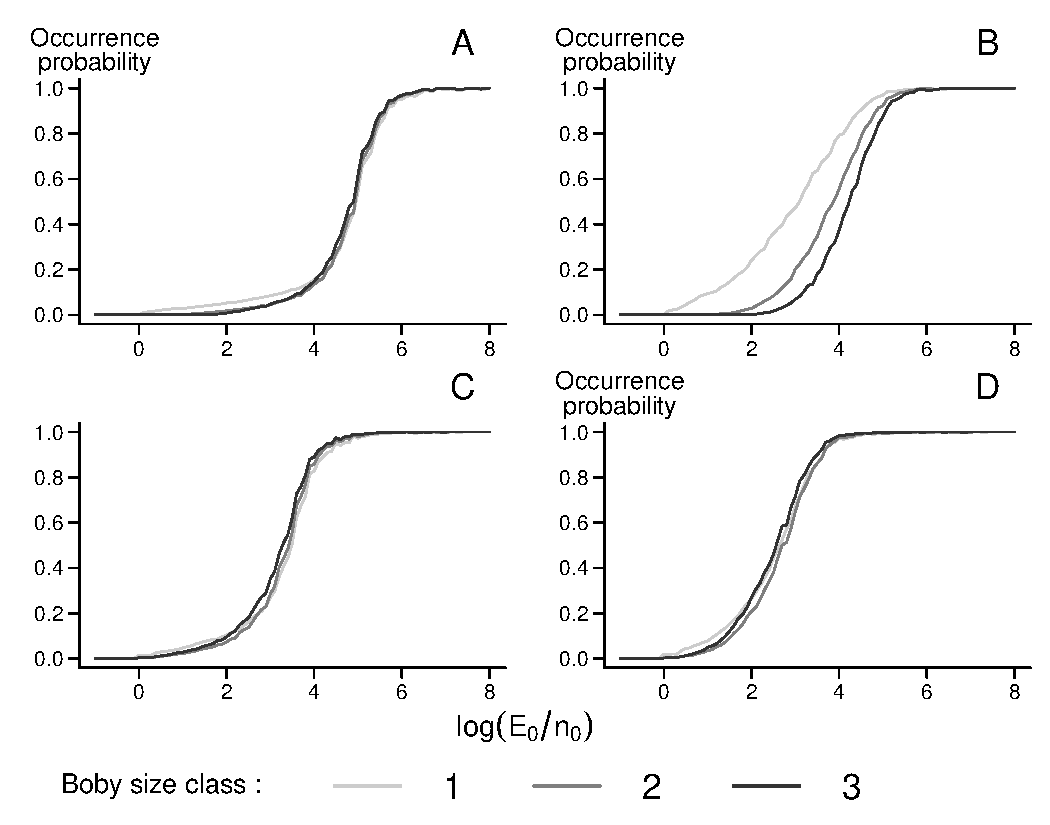
\includegraphics{chapitre4/fig/fig3.pdf}
\caption{\textbf{Species occurrence probability by energy gradient
grouped by body mass class}. The top right letters indicates the
scenarios.\label{fig:etib3}}
\end{figure}

\begin{figure}[htbp]
\centering
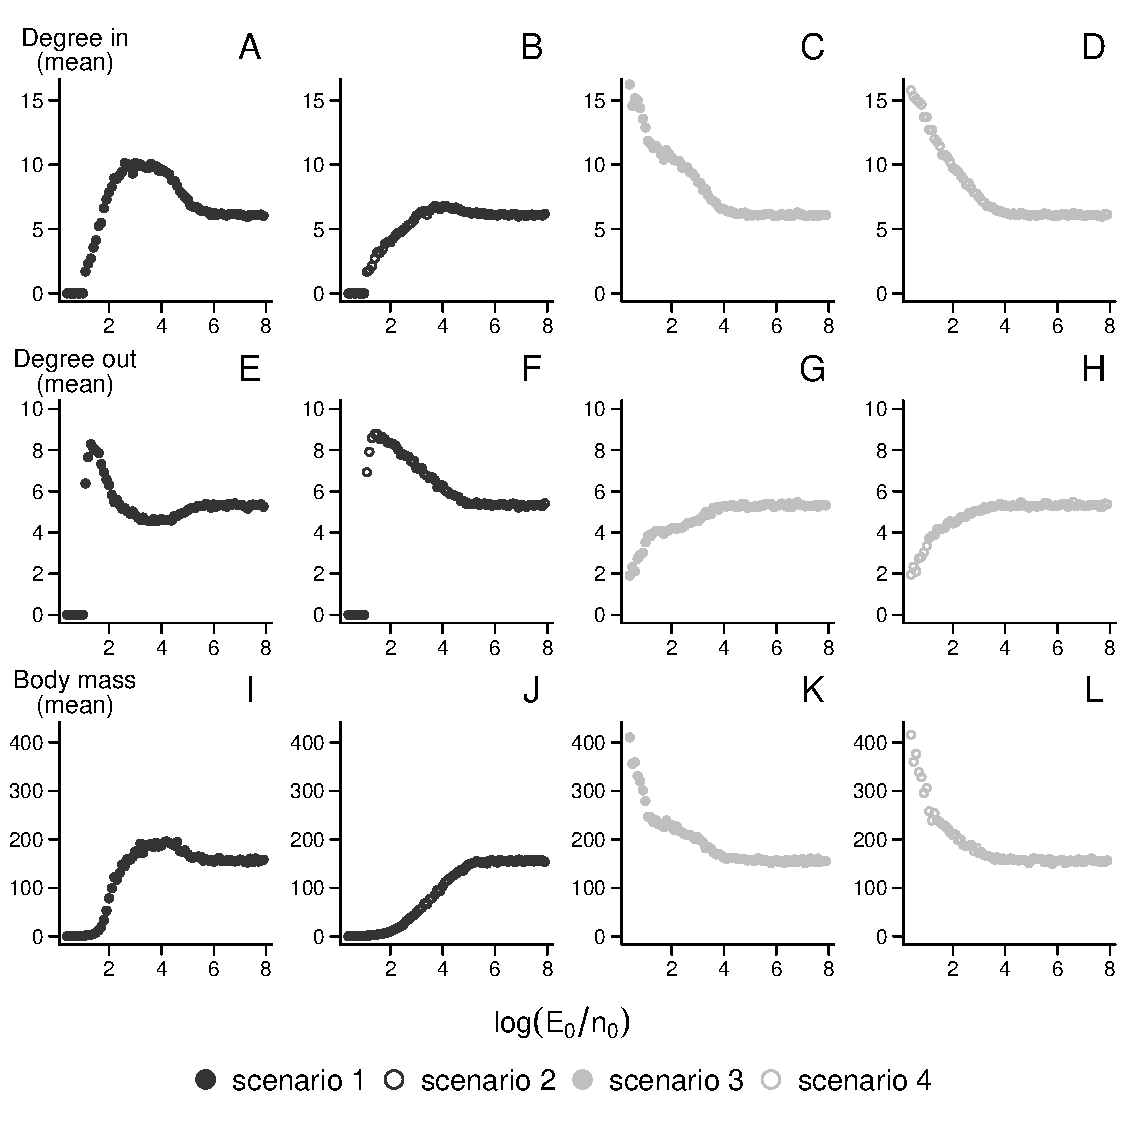
\includegraphics{chapitre4/fig/fig4.pdf}
\caption{\textbf{Average number of preys, predators, and mean body mass
of predator species on the island} in regards to the energy gradient for
four scenarios: (A) A,E,I, (B) B, F, J, (C) C, G, K, and (D) D, H,
L.\label{fig:etib4}}
\end{figure}


\cleardoublepage


\conclusion
\selectlanguage{french}
\section{Quelles type de prédicions pouvons nous faire
?}\label{quelles-type-de-pruxe9dicions-pouvons-nous-faire}

Bon objet et ce qui la concerne ou pas

problème de reflexion sur l'unité pertinente

des convergences contraintes physiques / intellegicence pour se
soustraire à la niche.. / la chitine

\subsection{Une question d'échelle}\label{une-question-duxe9chelle}

L'écologie porte sur l'ensemble du monde vivant quelquees soiten leur
taille mais les différent champs ne sont pas toutes relatoves à la
m\^{}me échelle alors il y a bien els échelles de temps, les echelles
spatiales mais il y a le lével d'organisation. Il est bien inportant de
comprendre cela !

Un scéhma avec des variables qui émergenet ave différemts paramères et
quelques éxemelpme de théorie! (DEB Evolution foodweb\ldots{}) et
l'action de

Repartition des especes des passges histroqiere dans l'origin des
espèces et dans Wallace. Le principe même de l'écologie (la definition
de ecologie).On arrive à l'idée de ;la niche. Exemple histriques. Dans
son ouvrage, le grand biogéographe Wallace reconait en introduction le
caractère facinant de la réaortition de la biodiversité des îles avec
des faot intriguant wuant à la faune et la flore. Ainsi il constate
qu'il peut y avir plus deux différence entre île très éloigné et deux
île s très proche. Il écrit que la faune et la flore sont plus
dissimilaire entre ldeles deux piles des Galapagos Bali et Lombik
qu'entre Hokaido (Yesso) et La grand bretagne ouy encore la Nouvelle
Zéland et l'Australie,

Exemple classique de grinnel et des Trasher + evolution avec les
charcter displacement.

Nous accumulons des évidences quand aux impact du changement
anthropique. A diiférentes échelles la diminution de la biodiversité,
changemnt en compoisiton Taranu et al. (2015) De Roos et al. (2008)

La biogéographie avec au moins 3 problèmes d'échelles =\textgreater{}
spatiale =\textgreater{} temporelle plus on augmente plus l'enpreinte
historiques est forte =\textgreater{} grands evenemnt géologique
(lacitaion mouvement des plques) biogéogrpahies historiqyes mais aussi
forme un pool d'espèces =\textgreater{} Mais aussi l'échelle taxonomique
: la relaton aire espèce est décrite à l'intérieru des taxons les
relations allométriques à l'inérieur des taxons E O Wilson a commencé à
rappporter des relation sur les formis les exemples du livre sont
herpeta faun (reptile plus amphibien) mecanisme =\textgreater{}
diversité de milieu

\subsection{Des classes d'esèces ?}\label{des-classes-desuxe8ces}

Wallace n'aurait-il pas eu plus de mal à comprndre les zones
aujourd'hui. Si naïvemnt on réduit aux villes, l'homogénéité ++ mais
avec les espèces invasive le signal est fortemnt briollé aussi !

Je pense qu'on est a un tournant de la biogoe vers un chamgemnt de
paradigme communaité centré qui ne nit pas les travaux précédant mais
les suit.

La défense des modèle climqtaiur bioclimate enveloppe de Pearson comme
une dpremière approximation utilise se faitt sur 3 exemple de plantes
Pearson and Dawson (2003)

\subsection{Prédire des
communautés}\label{pruxe9dire-des-communautuxe9s}

=\textgreater{} des interactions changer de paradigme

On nous fait miroiter que finalement que l'érosion de la biodiversité
est dramatiques et le ressort actuel pour faire un levier face à cela
c'est les services ecosystémiques qui sont actuelelemet l'argument choc
pour renforcer la production de la nature. Il y a un côté pervers qui
est la financiarisation et la substituabilité l'argent oeut alors être
utilisée pour intervertir ou alors remplacer un type d'écisystème par un
autre ailleurs\ldots{} En fait on a l'impressonq ue c'est pus un
principe de précaution qui erst invoquer et ultimement il est
vraisemblable que la destruction de la nature tel que nous la
connaissons soit dans le future un générateur de conflit\ldots{}. et
uttiment on a a craindre de faire un panete invivable pour nous mêm.
Mais les changement sont des remplacemnt et pour la conservation on peut
se demander les startégie. Dans son arctile `Don't juge a species on
their origin' Mark Davis prend à revers un sertain nombre d'idée recu et
souligne qye les effects des invedeurs peuvent être positives Davis et
al. (2011).

\section*{Vers une biogéographie
intégrative}\label{vers-une-bioguxe9ographie-intuxe9grative}
\addcontentsline{toc}{section}{Vers une biogéographie intégrative}

\subsection{Les données}\label{les-donnuxe9es}

Comme souvent en écolog/ie / science nous avons besoin de données, mais
ce n'est pas une qeustion vaine, L'Accumulation des données doit se
faire avec une certaine normalisation pour utiliser les. Il est souvent
difficile et la conséquence c'est de trouver des difficultés pour
réintégrer des anciennes données Tingley and Beissinger (2009) celle des
muséum Shaffer et al. (1998) Malgré les espoirs des remplacer les
ordinateurs pour formuler les hypothèse, toujours besoin d'un
développemnt théorique plus de que de corrélations essayer d'estimer
aujourd'hui en utilisant le plus près possible la méthode d'hier pour
savoir quel biais prbable il y avait. Ici si on détecte beaucoup plus
bas qu'avant avec la même méthode, alors on peut se dire que le fait que
ce soit des fausses absence est faible. Par contre si on essaye d'avoir
des comparaison et que les résultats sont du à la période de
l'année\ldots{} C'est plus compliqué ! Aller vers des occupancy model

\subsection{L'abstraction des
espèces}\label{labstraction-des-espuxe8ces}

\subsection*{Traits fonctionnels}\label{traits-fonctionnels}
\addcontentsline{toc}{subsection}{Traits fonctionnels}

Les traits fonctionnels sont des propriétés mesurables sur les
organismes en relation avec leurs performances et leur rôle dans
l'écosystème \cite{McGill2006}. Les traits étudiés peuvent être de
différentes natures, 1-morphologiques : taille de différentes parties du
corps, position des yeux, taille des oeufs chez les organismes ovipares,
taille des graines pour les végétaux, 2- physiologiques : taux
métaboliques de bases, stœchiométrie (rapport de la concentration entre
divers éléments qui compose l'organismes)
\cite{McGill2006,Albouy2011,Litchman2008}. Un ensemble approprié de ces
propriétés peut être un outil puissant pour décrire un ensemble d'espèce
dans un même espace. Leur proximité dans l'espace des traits est alors
un indice précieux d'une proximité fonctionnelle. Ainsi, à l'aide de 13
traits ecomorphlogiques, Albouy \textit{et al.} 2011 parviennent à
prédire les guildes trophiques de 35 espèces de poissons de la
Méditerranée \cite{Albouy2011}. Edwards \textit{et al.} 2013 montrent
que l'effet saisonnier sur une communauté de phytoplancton dans la
Manche peut être capturé à l'aide de traits décrivant : le taux maximal
de croissance, la compétitivité pour la lumière et l'azote
\cite{Edwards2013}. La distribution des traits fonctionnels au sein de
la biodiversité est aussi une entrée de choix pour réfléchir quand à la
fragilité potentielle des fonctions remplies par les écosystèmes
\cite{Mouillot2013}. \%DG: je comprends cette citation de Mouillot, mais
juste une mise en garde contre ce type de référence. Mouillot se base
sur l'hypothèse que les traits nous informent du fonctionnement, sans
jamais documenter cette relation. Ce qui est souvent le cas, et par
conséquent contribue à bâtir des mythes dans la littérature qui à
l'occasion ne sont pas toujours bien appuyés. L'approche par traits est
un bel exemple, on a édifié rapidement une structure conceptuelle sur
les traits, mais on n'a pas solidement appuyé le concept sur de bonnes
bases empiriques.

L'approche de la biodiversité par les traits fonctionnels est plus
quantitative que l'approche taxonomique et permet de déduire un grand
nombre de propriétés en se passant de la connaissance de leur identité.
Ainsi McGill, dans son article d'opinion de 2006, propose une approche
nouvelle de l'écologie des communautés qui transforme les questions
centrées autour des espèces par des questions qui interrogent la
répartition et la variabilité des traits \cite{McGill2006}. L'emploi des
traits fonctionnels est en fait un appel à une écologie plus mécaniste,
qui se penche sur la physiologie des organismes, en prend les faits les
plus importants (relativement au problème traité) pour les placer dans
un espace de traits commun. Cette approche est aussi en lien avec la
controversée théorie métabolique en écologie
\cite{Brown2004, Price2012}. Dans cette théorie un certain nombre de
grandeurs (comme le taux métabolique) sont reliées à la biomasse
corporelles de l'adulte, fournissant ainsi en un seul trait de
nombreuses relations pour des groupes d'organismes très différents. Par
ces nouvelles approches, l'espérance de s'extraire de la seule identité
des espèces est accrue, l'idée d'avoir des règles générales se
concrétise.

Dans une théorie intégrative de la biogéographie, les traits
fonctionnels peuvent être un pivot très intéressant pour rassembler les
différents concepts que nous avons développés dans les paragraphes
précédents. Les traits peuvent tout d'abord être mis en relation avec le
milieu abiotique. Le taux métabolique ou encore la sensibilité à la
sécheresse sont des indices performant pour décrire la survie dans un
milieu donné \cite{Kearney2004,Engelbrecht2007} que l'on peut capturer
sous forme de traits. Kearney \textit{et al.} 2010 propose une approche
prometteuse dans laquelle, l'environnement physique, la disponibilité
des ressources et la dynamique énergétique sont reliées par les traits
fonctionnelles le tout aboutissant à un modèle de distribution très
mécanistes. La structure d'un réseaux peut également être dérivée à
partir de l'espace des traits. Dans leur méthode proposée cette année,
Gravel \textit{et al.} infèrent les paramètres du modèle de niche de
Williams et Martinez \cite{Williams2000} à partir des relations de masse
du corps entre proie et prédateurs \cite{Gravel2013}. Ils sont alors en
mesure de dériver un réseau global pour un ensemble d'espèce donné.
Enfin, en tant qu'expression phénotypique, les traits fonctionnels sont
soumis aux processus évolutifs. Sur les temps longs, l'expression de
l'évolution résulte en la modification progressive des traits qui se
répercute sur l'ensemble des propriétés qui en découle. Ainsi la
considération d'une modification des traits est une approche simple et
réaliste pour introduire les processus évolutifs et leurs conséquences
\cite{Guill2008,Loeuille2005}.

L'abstraction de l'espèce Poisot et al. (2015) pour des questions
centrales : - quelles espceace av interagir avce qui ?\% Une chance pour
voir des communautés chnager et des communatés compltement affecté et en
tirer des conclusion ou alors le contraire des inférences des règles
valableque dans les milieux perturbés\ldots{} qui ont leur
règles\ldots{}

\subsection*{des prédictions fiables?}\label{des-pruxe9dictions-fiables}
\addcontentsline{toc}{subsection}{des prédictions fiables?}

\subsection*{Les dangers d'aller trop
vite}\label{les-dangers-daller-trop-vite}
\addcontentsline{toc}{subsection}{Les dangers d'aller trop vite}

\begin{quote}
There is also a danger that predictions grow faster than our
understanding of ecological systems, resulting in a gap between the
scientists generating the predictions and stakeholders using them
\end{quote}

``Predictive ecology in a changing world'' ({\textbf{???}})

\section*{Un monde en changement : entre espoir et
illusion}\label{un-monde-en-changement-entre-espoir-et-illusion}
\addcontentsline{toc}{section}{Un monde en changement : entre espoir et
illusion}

\subsection*{Une érosion de la biodiversité
affolantes}\label{une-uxe9rosion-de-la-biodiversituxe9-affolantes}
\addcontentsline{toc}{subsection}{Une érosion de la biodiversité
affolantes}

L'érosion de la biodiversité exergue une certaine nostalgie qui parfois
conduit une forme de fatalisme chez certain experts. Relevons la tête il
va falloir trouver les solutions dans le mimétisme ?

Alllant jusqu'à des porblèmes de santé La tique la souris le réservoir
et des hommes des problèmes de productions

\subsection*{Un monde biaisé?}\label{un-monde-biaisuxe9}
\addcontentsline{toc}{subsection}{Un monde biaisé?}

Sommes nous en train de biaisé le signal phylogénétique ? (cf article
Thuillier)

\subsection{Avons-nous des espoirs vains
?}\label{avons-nous-des-espoirs-vains}

Le royaume de la contingence du à l'impact historique de l'histoire
evolutive. Alors comment finder des espoinr de généralité quand le
moteur repose sur de la stochasticité Mais cette loi mène à des
prédictions exoecologie Les bactéries mais comment généraliser alors que
l'evolution à afit émerger bon nombre d'organisme qui en soi loin
quoique complèlemnt immbriqué on a plus de miro-organimes que de
cellules\ldots{}

inertie historique comment imaginer des plantes sans mycorrhyze mais
d'autres systeme auraiengt pu marcher En fait quand on pense à la plante
don pense à lMunité de lante + mycorrhuze et quand on pense à un
vertébrés on inclu tout ces bactérie on ne peut certes pas comprendre
comment l'un marche sans l'autre mais pour on a pas besoin de tout
connaître c'est un problème de rupture de symétrie.

Les conséquences sont compliqués des changements climatiques sont
nombreuses et certaines espèce voir le range grandir d'autre diminuer
pour cds espèce de co existent et donc à un changemnet prononc. de al
morphologoe des communautés alors que le nombre d'espèce peut être peu
affecté Moritz et al. (2008)

\subsection{DEB}\label{deb}

Le travail de Gotelli \textit{et al.} est également un exemple de
démarche intégrative où un nombre important de processus peuvent être
inclus via un système de combinaison de scénarios et tester par
simulations stochastiques \cite{Gotelli2009}. Enfin, en construisant des
réseaux basés sur la cooccurrence des espèces, Araújo \textit{et al.}
revisitent le problème de l'interdépendance des espèces
\cite{Araujo2011} : ils s'interrogent sur la résistance des réseaux de
cooccurrence obtenus face aux futurs changement climatiques, ils mettent
ainsi en évidence des risques accrus de perte des espèces les moins
connectés (celles qui cooccurent moins). Ces travaux témoignent de la
volonté d'une biogéographie intégrative.

C'est impressionnant de voir comment un auteur en repartant de simple
considération telle que la taile le volume peut arriver à construire une
théorie à la fois simple, fondée et predictive. mettant de la cohérence
dansune accumulation de fait.

=\textgreater{} problème SDMS quand inférencefait sur les données
d'espèces la force c'est d'avoir des mesures ++ et indépendante quelquee
part c'est vrai mais la source d'inforation est très brouillé et on peut
se demander se que l'on peut obtenir comme infornation\ldots{}.

Nous contraignons énormément les ranges d'espèces alors nous sort de
tout ça\ldots{}

L'ajout des interactions dans un modèle incluant l'environnement
abiotique interroge la relation que les deux processus entretiennent. Si
les espèces n'ont pas les mêmes performances dans différents milieux du
fait de leur physiologie, pour les mêmes espèces considérées, les
réseaux n'ont pas de raison d'être identiques d'un milieu à un autre.
C'est sur ce fait que Poisot \textit{et al.} 2012 ont proposé une mesure
de dissimilarité des réseaux \cite{Poisot2012}. Defossez \textit{et al.}
montrent que les interactions négatives entre l'hêtre commun
(\textit{Fagus Sylvaitca}) et les micro-organismes du sol diminuent avec
l'altitude \cite{Defossez2011}. Ainsi, les contraintes biotiques sont à
relier à l'environnement \cite{Brooker2006,Canham2006} et un modèle
intégratif doit donner un cadre cohérent à ces rétroactions entre
processus. Enfin, l'importance des interactions est à mettre en relation
avec l'échelle considérée \cite{Peterson2011}. Pour deux espèces en
interaction, plus l'échelle d'étude est large, moins les effets des
interactions locales sont susceptibles d'être capturés, le pouvoir
explicatif de la présence d'une espèce sur l'autre peut être alors
discutable \cite{Araujo2007}. Comprendre quels sont les processus à
prendre en compte aux différentes échelles spatio-temporelles et
comprendre comment le changement d'échelle affecte nous prédictions est
aussi un véritable challenge en biogéographie \cite{Martinez2012}.

A large espes répartition de la biodiversité on quantifie la différence
depuis les mesures classiques. Simpson, alpha gamma beta qui sont
étendues au réseau Poisot et al. (2012). Mais quand on chnage d'echelle
on arrive rarement à quelques choses de concluant pour l'integration des
interactions. Pourtant il ya des exemples convaicant comme celui de
Gitelli.

Le travail le plus dur devient d'utiliser un ensmeble de connaisance pur
déterminer des cartes de zone à risuqe mais la qualité des cartes est
théorie dépendant mais comprendre eavce pus de fiabiité les prochaines
zone ou \emph{Vespa} sera\ldots{}

\hypertarget{refs}{}
\hypertarget{ref-Davis2011}{}
Davis, M. a, Chew, M.K., Hobbs, R.J., Lugo, A.E., Ewel, J.J., Vermeij,
G.J., Brown, J.H., Rosenzweig, M.L., Gardener, M.R., Carroll, S.P.,
Thompson, K., Pickett, S.T. a, Stromberg, J.C., Del Tredici, P., Suding,
K.N., Ehrenfeld, J.G., Grime, J.P., Mascaro, J., Briggs, J.C., 2011.
Don't judge species on their origins. Nature 474, 153--4.
doi:\href{https://doi.org/10.1038/474153a}{10.1038/474153a}

\hypertarget{ref-DeRoos2008}{}
De Roos, A.M., Schellekens, T., Van Kooten, T., Persson, L., 2008.
Stage-specific predator species help each other to persist while
competing for a single prey. Proceedings of the National Academy of
Sciences of the United States of America 105, 13930--5.
doi:\href{https://doi.org/10.1073/pnas.0803834105}{10.1073/pnas.0803834105}

\hypertarget{ref-Moritz2008}{}
Moritz, C., Patton, J., Conroy, C., Parra, J., 2008. Impact of a century
of climate change on small-mammal communities in Yosemite National Park,
USA. Science 322, 261--4.
doi:\href{https://doi.org/10.1126/science.1163428}{10.1126/science.1163428}

\hypertarget{ref-Pearson2003}{}
Pearson, R.G., Dawson, T.P., 2003. Predicting the impacts of climate
change on the distribution of species: are bioclimate envelope models
useful? Global Ecology and Biogeography 12, 361--371.
doi:\href{https://doi.org/10.1046/j.1466-822X.2003.00042.x}{10.1046/j.1466-822X.2003.00042.x}

\hypertarget{ref-Poisot2012}{}
Poisot, T., Canard, E., Mouillot, D., Mouquet, N., Gravel, D., Jordan,
F., 2012. The dissimilarity of species interaction networks. Ecology
letters 15, 1353--61.
doi:\href{https://doi.org/10.1111/ele.12002}{10.1111/ele.12002}

\hypertarget{ref-Poisot2015}{}
Poisot, T., Stouffer, D.B., Gravel, D., 2015. Beyond species: why
ecological interactions vary through space and time. Oikos 124,
243--251. doi:\href{https://doi.org/10.1101/001677}{10.1101/001677}

\hypertarget{ref-Shaffer1998}{}
Shaffer, H., Fisher, R.N., Davidson, C., 1998. The role of natural
history collections in documenting species declines. Trends in Ecology
\& Evolution 13, 27--30.
doi:\href{https://doi.org/10.1016/S0169-5347(97)01177-4}{10.1016/S0169-5347(97)01177-4}

\hypertarget{ref-Taranu2015}{}
Taranu, Z.E., Gregory-Eaves, I., Leavitt, P.R., Bunting, L., Buchaca,
T., Catalan, J., Domaizon, I., Guilizzoni, P., Lami, A., Mcgowan, S.,
Moorhouse, H., Morabito, G., Pick, F.R., Stevenson, M.A., Thompson,
P.L., Vinebrooke, R.D., 2015. Acceleration of cyanobacterial dominance
in north temperate-subarctic lakes during the Anthropocene. Ecology
Letters 18, 375--384.
doi:\href{https://doi.org/10.1111/ele.12420}{10.1111/ele.12420}

\hypertarget{ref-Tingley2009b}{}
Tingley, M.W., Beissinger, S.R., 2009. Detecting range shifts from
historical species occurrences: new perspectives on old data. Trends in
Ecology and Evolution 24, 625--633.
doi:\href{https://doi.org/10.1016/j.tree.2009.05.009}{10.1016/j.tree.2009.05.009}

\cleardoublepage





% ----------------------------------------------------------------------%
% 4 - Appendices de la thèse.                                           %
% ----------------------------------------------------------------------%


\selectlanguage{french}
\appendice{Comment la biodiversité s'installe en territoires isolés}
\label{annI}
\addtocounter{chapter}{1}
\setcounter{equation}{0}


L'article qui suit est le fruit de ma rencontre avec Philippe Etchécopar,  membre du comité éditorial du journal \emph{Accro$\alpha$mth}.
Ce journal de vulgarisation mathématique est destiné aux étudiants et enseignants en mathématiques du Cégep\footnote{Le cégep est la dernière étape avant l'entrée à l'université pour ceux désirant poursuivre leurs études.}.
Dans cet article, je reprends les bases du modèle de la TIB et je montre comment en partant d'une équation simple sur les probabilités, il est possible d'obtenir une équation différentielle déterministe. L'article est accessible en ligne\footnote{http://accromath.uqam.ca/2014/02/la-biodiversite-en-territoires-isoles}


\section{Préambule}
	La biogéographie est la science qui s’interroge sur les causes de la répartition de la biodiversité dans les différentes parties du globe (voir encadré 1). Le modèle déterministe de MacArthur et Wilson décrit l’évolution de la richesse spécifique sur les îles vers un équilibre, mais la migration des espèces vers des îles et leur extinction potentielle sont des phénomènes aléatoires. Comment un modèle déterministe peut-il renfermer ce hasard? C’est ce que nous allons voir.

\section{Le modèle de MacArthur et Wilson}

Un des modèles les plus puissants en biogéographie est celui proposé par MacArthur et Wilson dans leur passionnante théorie de la biogéographie des îles. Ces deux illustres prédécesseurs nous ont livré un paradigme simple et puissant pour envisager la construction de la biodiversité sur une île. Notons dès maintenant que l'île n'est pas nécessairement un monticule de sable fin au milieu de l'océan mais plutôt -et plus généralement- un territoire isolé. Le modèle permet de comprendre l'impact des capacités de dispersion et de survie des espèces sur la biodiversité $S$ de l'île considérée. Considérons que cette île est accessible depuis un continent qui présente un ensemble constant d'espèces $P$. Les $P$ espèces sont potentiellement celles que nous retrouverons sur l'île, nous avons donc $S\leqslant P$. À un temps $t$ donné, l'ensemble des $S$ espèces de l'île peuvent s'éteindre avec un taux $e$. De même, les $P-S$ espèces du continent (absentes de l'île) peuvent coloniser l'île avec un taux $c$. En langage mathématique, nous obtenons l'équation différentielle déterministe suivante pour décrire l'évolution temporelle de $S$~:
\begin{eqnarray}
\nonumber \frac{dS}{dt}&=&c(P-S)-eS\\
\label{eqAnnI1} &=&cP-(c+e)S
\end{eqnarray}
Cette équation est linéaire, nous pouvons la résoudre facilement par la méthode de la variation de la constante (essayez puis regardez l'encadré 2!). Pour les valeurs arbitraires $c=0.2$, $e=0.1$ et la condition initiale suivante~: à $t=0$, l'île est inhabitée ($S(0)=0$), nous représentons graphiquement la solution de l'équation à la figure \ref{figAnnI1}. Pour un temps infini, la biodiversité tend vers la valeur~: $S_{eq}=P\left(\frac{c}{c+e}\right)$, interprétée comme le nombre d'espèces provenant du continent et présentes sur l'île à l'équilibre.

\begin{figure}[h!]
\centering
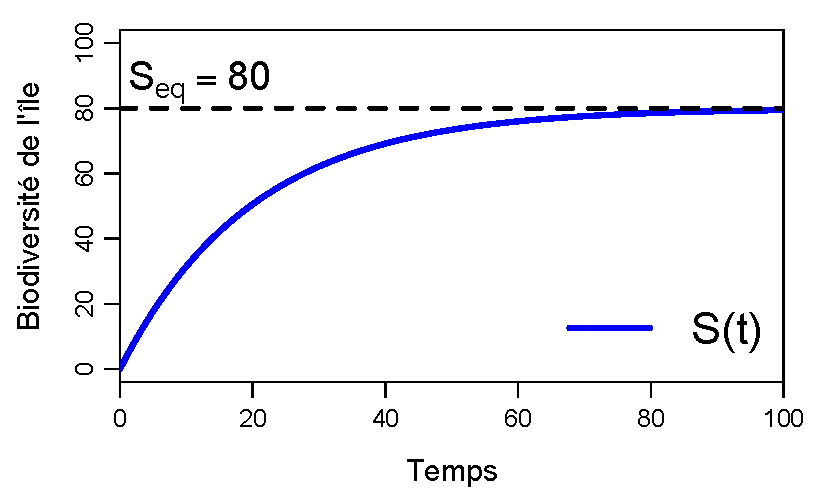
\includegraphics[width=0.9\textwidth]{annexe1/fig/figAnnI1.pdf}
\caption[Représentation graphique de la solution de l'équation différentielle]{\textbf{Représentation graphique de la solution de l'équation différentielle} \eqref{eqAnnI1} pour les conditions suivantes~: $c=0.04$, $e=0.01$ et $S(0)=0$. La ligne en pointillés représente la valeur de la biodiversité $S_{eq}$ que nous obtenons à un temps infini.}
\label{figAnnI1}
\end{figure}



\section{Comment un modèle déterministe émerge-t-il de phénomènes aléatoires?}

\subsection{Modèle stochastique?}
Il est très intéressant de réaliser que l'équation \eqref{eqAnnI1}, d'apparence déterministe, renferme un modèle stochastique. "Stochastique" est un terme signifiant aléatoire, avec une part de hasard. Un modèle stochastique est donc un modèle dont l'issue contient une part de hasard; deux réalisations du modèle ne donneront donc pas nécessairement le même résultat. Pour comprendre où se cache le hasard dans le modèle que nous étudions, nous avons besoin d'objets mathématiques particuliers appartenant au domaine des probabilités~: variables aléatoires et processus stochastiques (reportez-vous à l'encadré 3).

\subsection{Les objets mathématiques requis}
Comment savoir combien d’espèces sont présentes sur l’île ? Il suffit de compter 1 pour chaque espèce présente sur l’île. Nous introduisons donc $X_i$ , la variable aléatoire de présence sur l’île de l’espèce $i$ choisie parmi les $P$ espèces du continent. $X_i$ est égale à 0 si l’espèce n’est pas sur l’île et 1 si elle est sur l’île. C’est une variable aléatoire de Bernoulli (encadré 4). Ainsi, le nombre d’espèces présentes sur l’île, $S$, est égale à la somme des $X_i$. Nous allons encore plus loin en enregistrant ces valeurs au cours du temps. C'est ainsi que nous définissons le processus stochastique $X_{i,t>0}$, qui n'est autre qu'une succession de 1 et de 0 indiquant à chaque instant si oui ou non l'espèce $i$ est sur l'île. A priori, les suites $X_{i,t}$ ne sont pas prévisibles, ce qui n’exclut pas que la fonction $S$ présente, en moyenne, un comportement tout à fait régulier.

\subsection{Les briques élémentaires du modèle stochastique}
Au temps $t=0$, l'espèce $i$ n'est pas sur l'île. Pour construire la suite de son histoire, il nous faut une règle simple pour décrire l'évolution de sa présence entre deux pas de temps très proches. Le modèle de MacArthur et Wilson postule que si l'espèce considérée est sur l'île au temps $t$, elle s'éteint avec un taux $e$ ; si elle est sur le continent, elle le colonise avec un taux $c$. Pour simplifier, nous supposerons que les taux d’extinction et de colonisation sont les mêmes pour toutes les espèces. Nous donnons maintenant une signification en terme de probabilité à ces taux~: $c$ est la probabilité de colonisation par unité de temps (on parle de densité du processus), $e$ est la probabilité d'extinction par unité de temps. Ainsi, $edt$ désigne la probabilité d'extinction pendant l'intervalle de temps $dt$. De même, $cdt$ est la probabilité de colonisation pendant $dt$. En faisant appel aux probabilités conditionnelles (encadré 5), en supposant $dt$ assez petit, nous différencions quatre cas:
\begin{eqnarray}
 \label{eqAnnI3a}  \forall t \in \mathbb{R}^+, ~~P(X_{i,t+dt}=1|X_{i,t}=0)&=&cdt\\
 \label{eqAnnI3b} P(X_{i,t+dt}=0|X_{i,t}=1)&=&edt \\
 \label{eqAnnI3c} P(X_{i,t+dt}=0|X_{i,t}=0)&=&(1-cdt) \\
   \label{eqAnnI3d} P(X_{i,t+dt}=1|X_{i,t}=1)&=&(1-edt)
\end{eqnarray}
Il faut comprendre la première équation ainsi~: sachant que l'espèce $i$ était absente au temps $t$, la probabilité qu'elle soit sur l'île au temps $t+dt$ est égale à la probabilité qu'elle colonise l'île durant $dt$, c'est-à-dire $cdt$. Vous pourriez avancer que durant $dt$, une espèce peut coloniser, s'éteindre et re-coloniser et que nous n'en parlons pas ! Tous ces évènements sont en fait beaucoup moins probables et nous pouvons les ignorer complètement à la limite quand dt tend vers 0. Les trois autres équations s'interprètent avec un raisonnement similaire. Ces quatre équations sont les briques du modèle stochastique que nous construisons. Nous devons maintenant les assembler correctement.


\subsection{Assemblons les briques!}

L'assemblage consiste en l'utilisation de la formule des probabilités totales expliquée dans l'encadré 5. Nous pouvons en déduire la probabilité de présence de l'espèce $i$ à l'instant $t+dt$~:
\begin{eqnarray}
\nonumber P(X_{i,t+dt}=1)&=&P(X_{i,t+dt}=1|X_{i,t}=0)P(X_{i,t}=0) \\
\label{eqAnnI4}  & &+P(X_{i,t+dt}=1|X_{i,t}=1)P(X_{i,t}=1)
\end{eqnarray}
Il s'agit d'une somme de deux termes couvrant toutes les possibilités puisque, à l'instant $t$, l'espèce $i$ était soit absente de l'île soit présente, c'est un système complet d'évènements (encadré 5). Si l'espèce $i$ était absente (premier terme) à $t$, elle sera présente à $t+dt$ si elle colonise pendant $dt$ \eqref{eqAnnI3a}. Si elle était déjà sur l'île à $t$, elle s'y maintient à condition de ne pas s'éteindre \eqref{eqAnnI3d}. En remarquant que $P(X_{i,t}=0)=1-P(X_{i,t}=1)$, nous pouvons écrire~:
\begin{eqnarray}
\label{eqAnnI5a} P(X_{i,t+dt}=1)&=&cdt(1-P(X_{i,t}=1))+(1-edt)P(X_{i,t}=1)
\end{eqnarray}
Pour simplifier l'écriture, $s_{i,t}$ représente $P(X_{i,t}=1)$~:
\begin{equation}
\label{eqAnnI5b} s_{i,t+dt}=cdt(1-s_{i,t})+(1-edt)s_{i,t}
\end{equation}
Divisons par $dt$~:
\begin{eqnarray}
\label{eqAnnI5c} \frac{s_{i,t+dt}-s_{i,t}}{dt}&=&c(1-s_{i,t})-es_{i,t}
\end{eqnarray}
Nous faisons alors tendre $dt$ vers 0. Nous obtenons alors~:
\begin{equation}
\label{eqAnnI5e} \frac{ds_{i}}{dt}=c(1-s_{i})-es_{i}
\end{equation}
C'est l'équation que nous avons résolu dans l'encadré 1, avec $P=1$~:
\begin{equation}
\label{eqAnnI5e} s_{i}(t)=\frac{c}{c+e} \left(1-\exp{(-(c+e)t)}\right)
\end{equation}

\subsection{Retrouvons le modèle classique}
Nous avons presque retrouvé la solution de l'équation déterministe; vous pourriez penser qu'il faut simplement multiplier par le nombre d'espèces $P$. L'idée est bonne, mais demande justification ! Nous allons effectivement considérer non pas une mais bien les $P$ espèces du continent pour lesquelles l'équation \eqref{eqAnnI5e} est valable. Nous allons alors définir un nouveau processus stochastique qui est simplement la somme des $P$ processus de présence que nous supposons indépendants $X_{i,t>0}$, $Y_t>0=X_{1,t>0}+X_{2,t>0}+....X_{P,t}$. Le problème est alors de connaître à tout instant $t$ la probabilité d'avoir un nombre donné $k$ d'espèces présentes sur l'île. À un instant donné $t$ nous faisons une somme de variable aléatoires de Bernoulli. La somme de $P$ variables de Bernoulli indépendantes est une variable aléatoire suivant une loi binomiale (encadré 5). Nous avons donc~:
\begin{equation}
 \forall t \in \mathbb{R}^+, ~~\label{eqAnnI6a} P(Y_t=k)=\binom{P}{k}s(t)^k(1-s(t))^{P-k}
\end{equation}
De plus, on peut démontrer les résultats suivants~:
\begin{eqnarray}
 \forall t \in \mathbb{R}^+, ~~\label{eqAnnI6b} E(Y_t)&=&Ps(t) \\
 \forall t \in \mathbb{R}^+, ~~\label{eqAnnI6c} V(Y_t)&=&Ps(t)(1-s(t))
\end{eqnarray}
Grâce à ces résultats de probabilité, nous avons donc~:
\begin{equation}
 \forall t \in \mathbb{R}^+, ~~\label{eqAnnI6d} E(Y_t)=P\frac{c}{c+e}(1-\exp(-(c+e)t))
\end{equation}

Nous retrouvons la solution déterministe! Ainsi, le modèle déterministe peut être considéré comme reflétant l'évolution de l'espérance des variables $Y_t$ pour $t>0$, c'est donc l'espérance du processus stochastique. Nous pouvons alors simuler le modèle stochastique grâce au modèle déterministe~: à chaque instant $t$, il suffit de simuler une loi binomiale de paramètres $P$ et $E(Y_t)$. Regardez la figure \ref{figAnnI2}, il y a des différences fondamentales entre les deux approches. Le modèle déterministe donnera des valeurs continues et, pour des paramètres donnés, toujours le même résultat. De son côté, le modèle stochastique livrera des valeurs discrètes. De plus, deux simulations du modèle aléatoire ne donneront pas nécessairement les mêmes courbes.

\begin{figure}[h!]
\centering
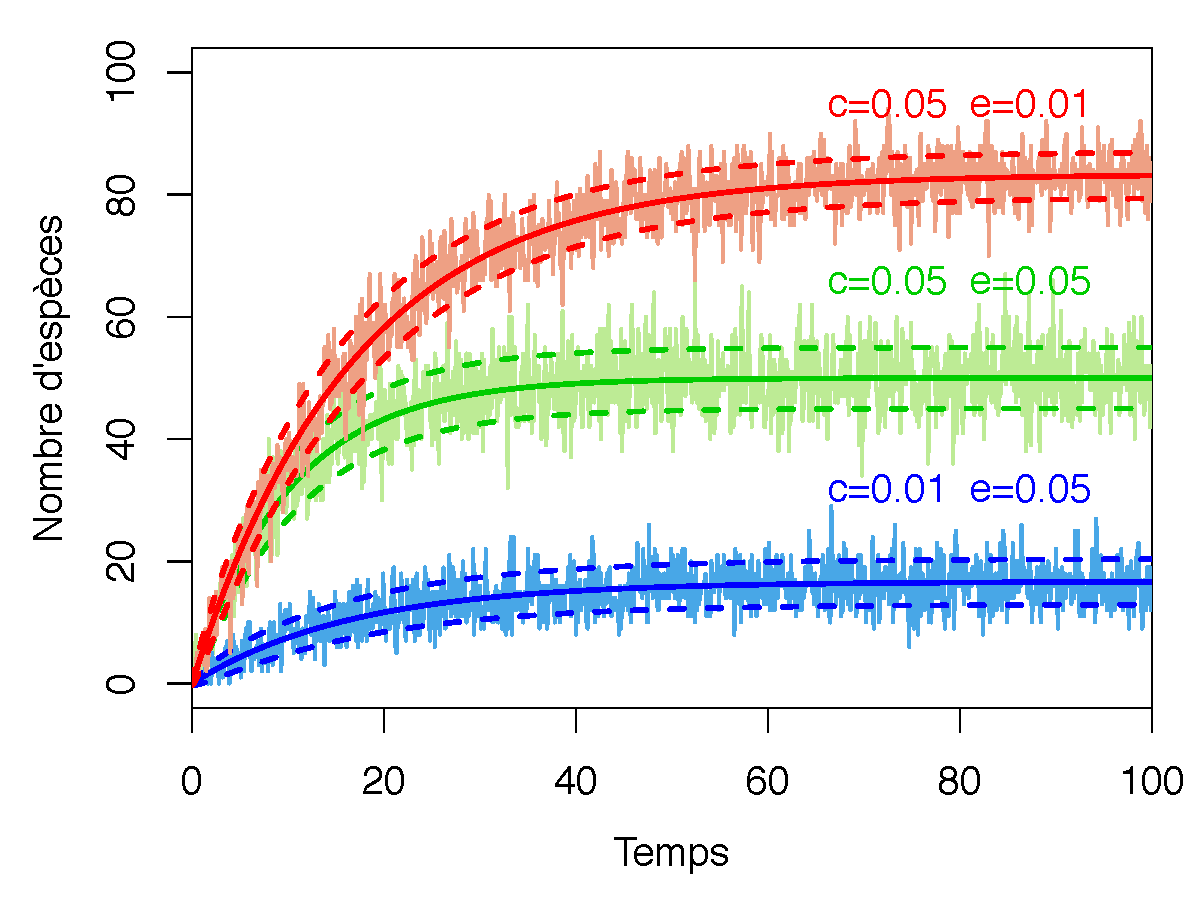
\includegraphics[width=0.9\textwidth]{annexe1/fig/figAnnI2.pdf}
\caption[Dynamique de la biodiversité de trois zones protégées]{\textbf{Dynamique de la biodiversité de trois zones protégées}. Les caractéristiques de la zone protégée sont données par les valeurs de $c$ et $e$. Les symboles rouges sont relatifs à une zone protégée de grande taille et facilement accessible, en vert, ils font référence à une petite zone facilement accessible ; enfin, en bleu, sont présentées les résultats pour une petite zone difficilement accessible. Les courbes striées en couleurs pastels sont les réalisations du modèle stochastique. Les courbes en traits pleins, font référence au modèle déterministe qui est également la moyenne du modèle stochastique. Enfin, les courbes en pointillés représentent la moyenne du modèle stochastique plus ou moins l'écart type.}
\label{figAnnI2}
\end{figure}



\section{Applications et perspectives}

Bien que datant du milieu des années 1960, le modèle de MacArthur et Wilson demeure très précieux, notamment pour étudier les habitats fragmentés (des îles!) et prendre des décisions relatives à la conservation des espèces. Prenons un exemple~: vous êtes le gestionnaire d'une nouvelle zone protégée que nous assimilerons à une île. Cette zone a longtemps été exploitée par l'homme de sorte qu'au temps $t=0$ le nombre d'espèces est $S=0$. Dans la région, la richesse en espèces est de $P=100$, c'est-à-dire que vous pouvez rencontrer jusqu'à 100 espèces dans votre aire de gestion. À la suite de MacArthur et Wilson, nous allons supposer que la valeur du taux de colonisation $c$ dépend de la difficulté d'accès. De plus, la survie d'une espèce sur cette zone dépend de sa superficie~: ainsi plus l'aire de conservation est grande, moins les espèces s'éteignent; $e$ est donc plus faible pour les grandes aires de protection. Prenons trois situations~:
\begin{itemize}
\item Grande zone et accès aisé~: e=0.01 et c=0.05
\item Petite zone et accès aisé~: e=0.05 et c=0.05
\item Petite zone et accès délicat~: e=0.05 et c=0.01
\end{itemize}
Pour mettre en place un suivi et savoir comment se comporte votre réserve, il faut avoir une idée de la dynamique attendue ! Ce que nous permet le modèle étudié, que nous simulons pour les trois situations, avec les deux approches du modèle. Les résultats sont donnés par la figure 1. Cette simple démarche vous permet d'estimer l'évolution de la biodiversité au sein de votre réserve. La paramétrisation est plus compliquée dans les faits, mais l'idée est très utilisée pour apprécier la santé des réserves naturelles.


Dans cet exemple, le modèle stochastique n'a finalement que peu d'intérêt. Il est cependant très utile si vous êtes intéressé par la variance du modèle (que nous obtenons avec l'équation \eqref{eqAnnI6c}). C'est aussi un bon point de départ pour les démarches statistiques, indispensables pour le suivi de votre réserve. De plus, l'approche stochastique révèle toute sa force pour enrichir le modèle. En partant de l'équation \eqref{eqAnnI1}, si vous souhaitiez introduire un effet des espèces les unes sur les autres (les interactions entre espèces), vous auriez quelques difficultés. Avec le travail réalisé ici vous pouvez trouver et surtout justifier des approches fertiles en réfléchissant en terme de probabilité. Ces approches pourraient vous amener à résoudre des systèmes d'équations différentielles déterministes un peu plus compliqués~!


\newpage

\setlength{\columnsep}{1cm}
\begin{minipage}{0.9\linewidth}
\textbf{Encadré 1~: la Biogéographie} \\
	La biogéographie est la science qui s'interroge sur les causes de l'agencement spatial des espèces à la surface de notre planète. Comment, par exemple, pouvons-nous expliquer la répartition et les différences entre les grands biomes terrestres? Le premier élément de réponse est l'implication des facteurs climatiques. La température, l'humidité, les précipitations sont autant de variables qui contraignent les conditions d'existence des espèces qui composent et modèlent les paysages terrestres. C'est avec ces contraintes que les écologues élaborent des modèles dits "bioclimatiques" afin de décrire l'évolution de la biodiversité avec les contraintes climatiques de demain. Cependant, les facteurs qui expliquent la distribution des espèces ne sont pas toujours climatiques, les causes sont multiples. Les mouvements des espèces et leurs histoires évolutives sont ainsi des moteurs fondamentaux en biogéographie. Les capacités de dispersion des espèces leur donnent accès à de nouveaux territoires qui, avec le temps peut-être, les verront disparaître. C'est ainsi qu'un territoire voit sa composition en espèces évoluer, avec l'arrivée de nouvelles espèces et l'extinction d'autres. C'est autour de cette idée majeure que s'articule le modèle présenté.
\end{minipage}
\vspace{2cm}

\setlength{\columnsep}{1cm}
 \begin{minipage}{0.9\linewidth}
 \begin{multicols}{2}
 \textbf{Encadré 2} \\
 Il est facile de vérifier que la solution générale de l’équation homogène~:
 \begin{equation}
\nonumber  \frac{dS}{dt}=-(c+e)S
\end{equation}
est donnée par~:
 \begin{equation}
\nonumber \forall t \in \mathbb{R}^+,~ S(t)=C\exp(-(c+e)t)
\end{equation}
où $C$ est une constante, la solution de l’équation non homogène est alors de la forme~:
 \begin{equation}
\nonumber S(t)=f(t) \exp(-(c+e)t)
\end{equation}
En remplaçant dans l’équation différentielle on obtient~:
 \begin{equation}
\nonumber f’(t) \exp(-(c+e)t)= cP
\end{equation}
ce qui nous donne~:
 \begin{equation}
\nonumber f’(t)= cP \exp((c+e)t)
\end{equation}
En intégrant on obtient~:
 \begin{equation}
\nonumber f(t)= P\frac{c}{c+e} \exp({(c+e)t}) + K
\end{equation}
où $K$ est une constante arbitraire.
 \begin{equation}
\nonumber S(t)= P\frac{c}{c+e} + K\exp(-(c+e)t)
\end{equation}
Avec $S(0)=0$, $K=-P\frac{c}{c+e}$, nous obtenons donc~:
 \begin{equation}
\nonumber S(t)= P\frac{c}{c+e} (1-\exp(-(c+e)t))
\end{equation}
\end{multicols}
 \end{minipage}
\vspace{2cm}

\setlength{\columnsep}{1cm}
 \begin{minipage}{0.9\linewidth}
\textbf{Encadré 3} \\
Les \textbf{variables aléatoires} sont des fonctions définies sur l’ensemble des résultats possibles d’un événement aléatoire. Comme le résultat de l’événement est aléatoire, on associe à chaque valeur de la variable sa probabilité, de sorte que la somme des probabilités sur l'ensemble des valeurs possibles soit égale à 1. Dans notre exemple, $X_i$ est une variable aléatoire, 0 et 1 sont ses valeurs, et nous nous intéressons à leur probabilité $P(X_i=1)$ et $P(X_i=0)$ avec $P(X_i=1)+P(X_i=0)=1$. \\
Les \textbf{processus aléatoires ou stochastiques} sont des collections de variables aléatoires indexées par le temps $t$, c'est-à-dire ordonnées. Dans notre exemple, l'indexation est faite selon le temps $t$. Nous suivons ainsi l'évolution de $X_i$ au cours du temps d'où la notation $X_{i,t>0}$. Attention ! $X_{i,t>0}$ est un processus aléatoire mais $X_{i,t}$ est l'une des variables aléatoires du processus.
 \end{minipage}
\vspace{2cm}

\setlength{\columnsep}{1cm}
 \begin{minipage}{0.9\linewidth}
 \textbf{Encadré 4} \\
Une variable aléatoire $X$ suit un \textbf{schéma de Bernoulli} lorsqu'elle prend uniquement deux valeurs 0 ou 1. Si nous notons $p=P(X=1)$, nous avons~:
\begin{itemize}
\item $P(X=0)=1-p$
\item $E(X)=p$
\item $V(X)=p(1-p)$
\end{itemize}
$X$ est alors une variable aléatoire de Bernoulli de paramètre $p$. \\
Une variable aléatoire $X$ suit une \textbf{loi Binomiale} de paramètres $n\in\mathbb{N}$ et $p\in[0,1]$ lorsqu'elle est la somme de $n$ variables de Bernoulli indépendantes de paramètre $p$. On peut alors montrer les résultats suivants~:
\begin{itemize}
\item $\forall k \leq n,~ P(X=k)=\binom{n}{k}p^k(1-p)^{n-k}$
\item $E(X)=np$
\item $V(X)=np(1-p)$
\end{itemize}
 \end{minipage}
\\  \\  \\


\begin{figure}[H!]
\centering
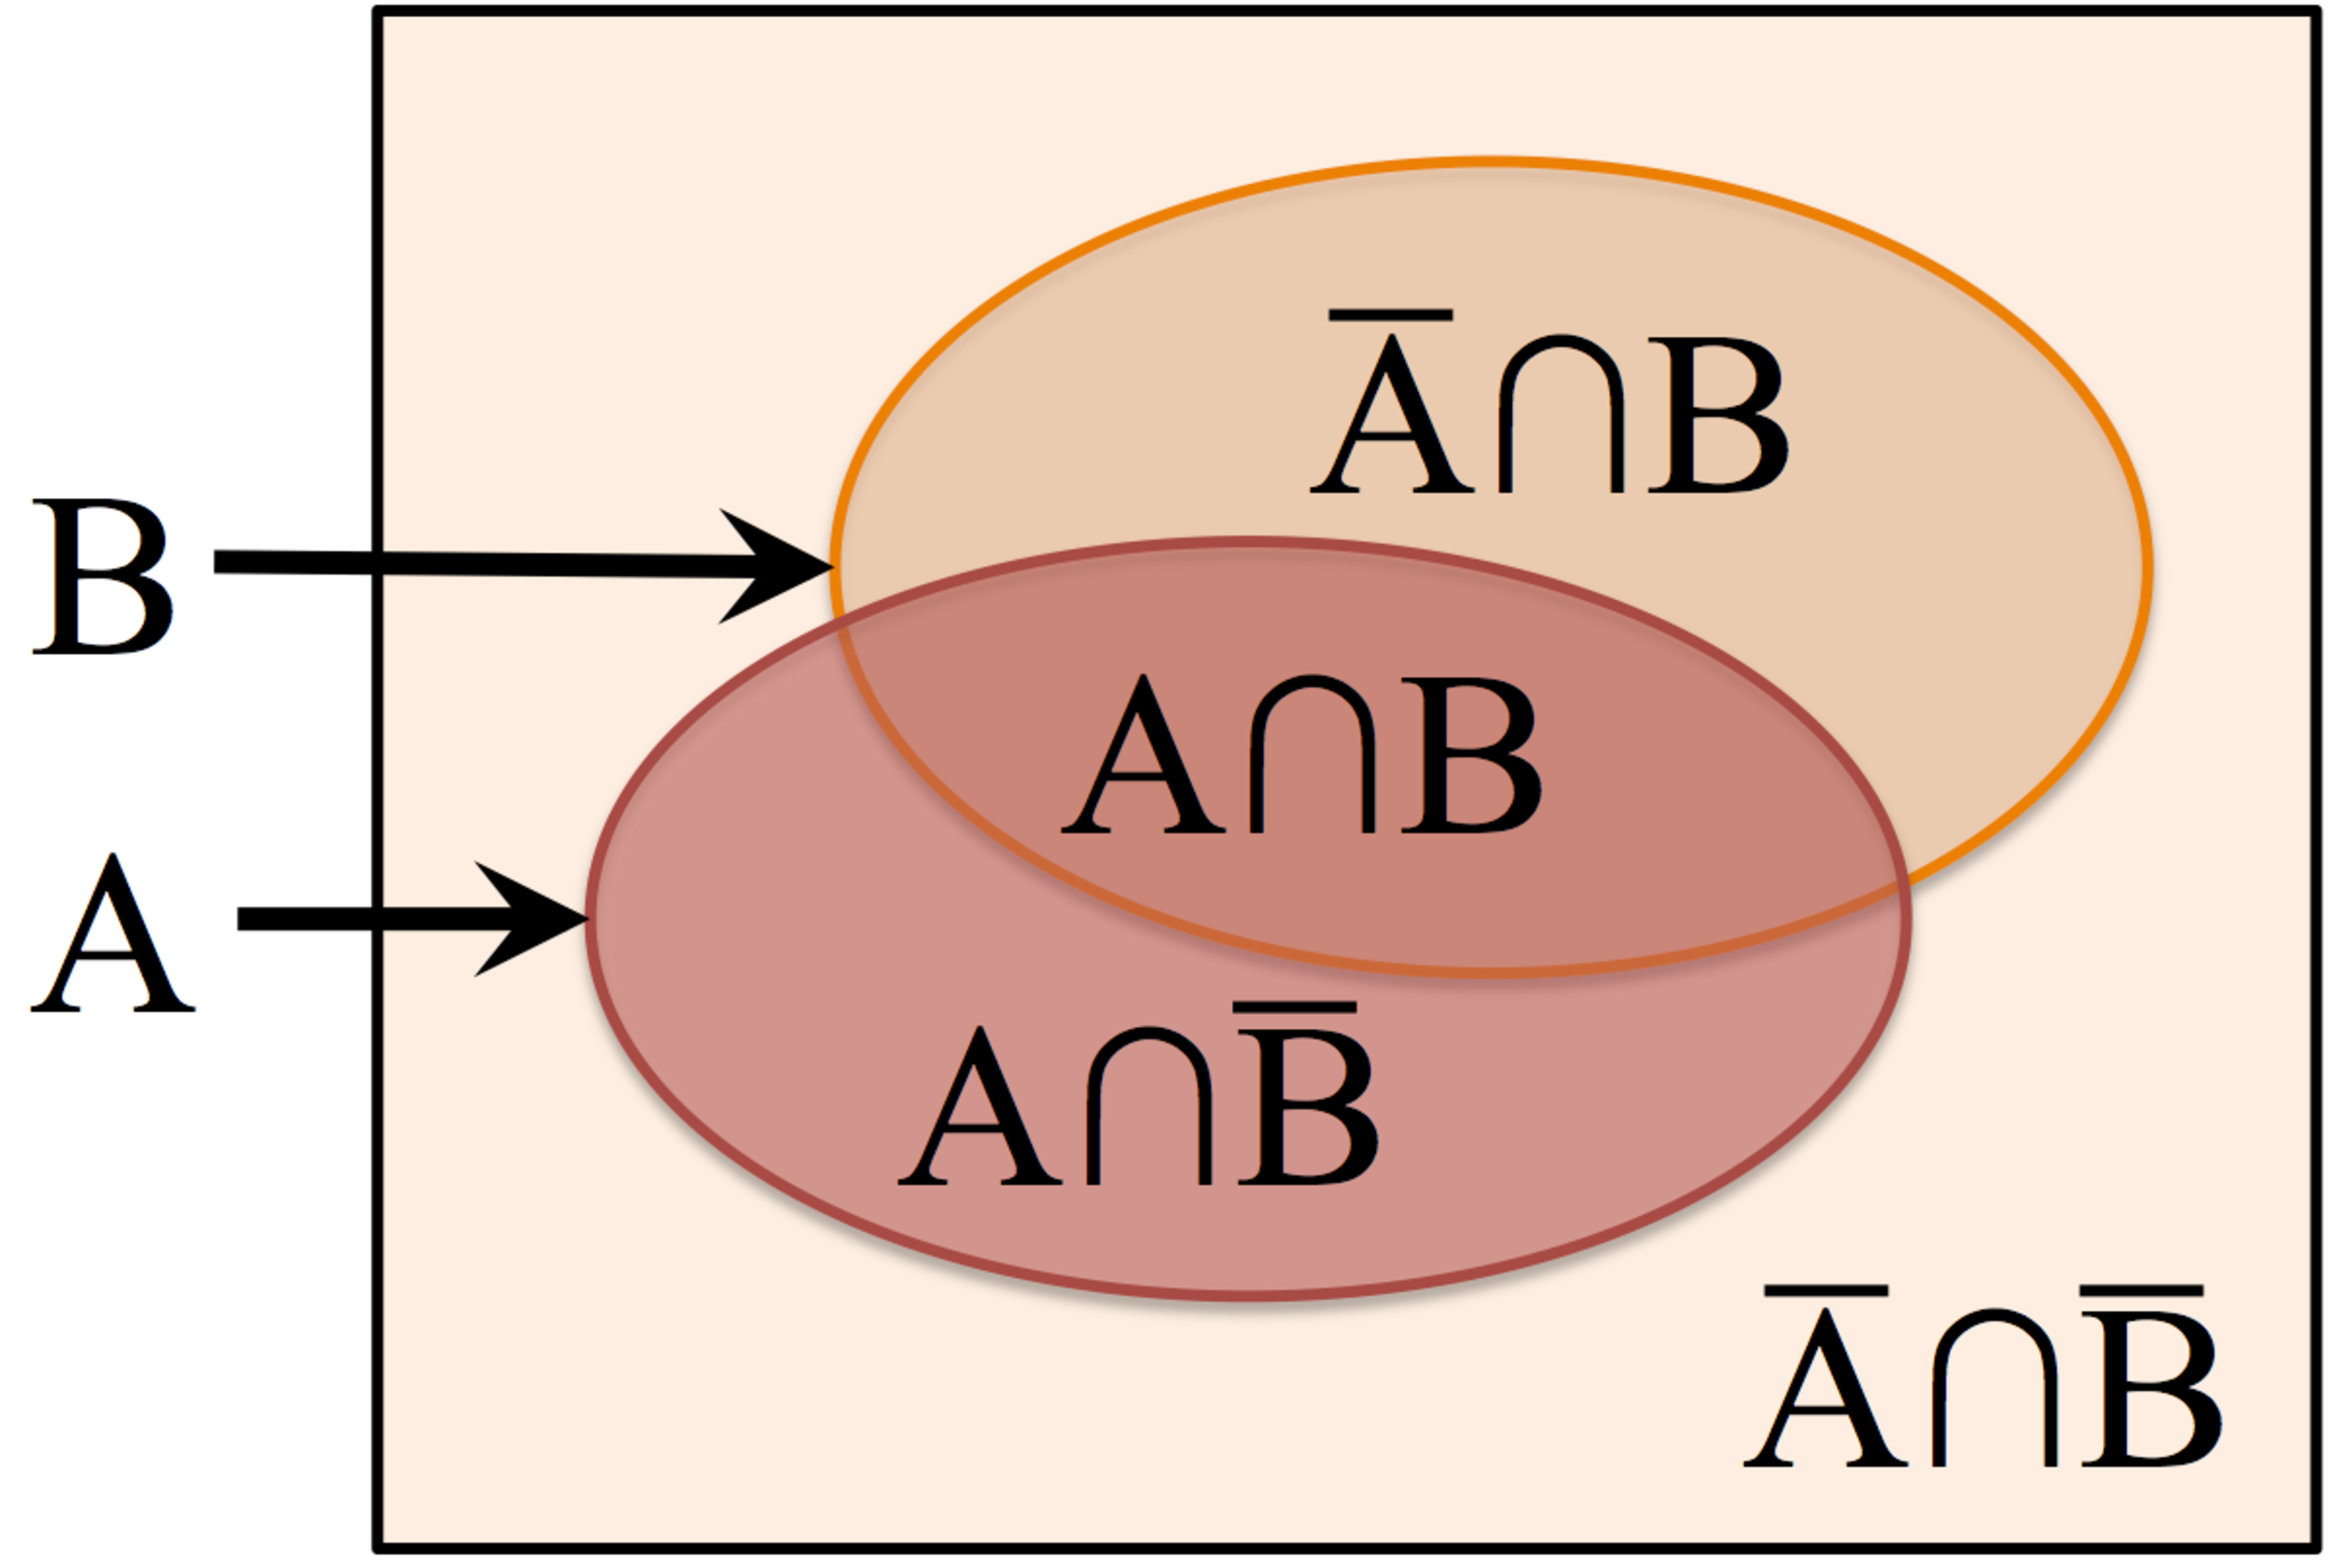
\includegraphics[width=0.95\textwidth]{annexe1/fig/figAnnI3.pdf}
\caption[Représentation de la formule des probabilités totales.]{\textbf{Représentation de la formule des probabilités totales}. $A$ et $B$ sont deux événements. La probabilité de A peut être décrite comme la somme de l'intersection avec $B$ et $\bar B$ qui constituent un système complet d'évènements.}
\label{dess1}
\end{figure}

\newpage


\setlength{\columnsep}{1cm}
\begin{minipage}{0.9\linewidth}
\textbf{Encadré 5} \\
Une \textbf{probabilité conditionnelle}, est une probabilité qu'un évènement se réalise à condition qu'un autre soit déjà réalisé. Soit deux évènements $A$ et $B$, la probabilité de $A$ sachant $B$, notée ici $P(A|B)$ est la probabilité que $A$ se réalise lorsque B est réalisé. \\
Un \textbf{système complet d'évènements} est un ensemble d'événements exclusifs dont la somme des probabilités est 1. Par exemple, l'évènement $B$ et son complémentaire $\bar{B}$ forme un tel système (voir figure \ref{dess1}).\\
La \textbf{formule des probabilités totales} nous donne la probabilité de réalisation d'un évènement à partir de la connaissance de probabilités conditionnelles sous réserve que l'ensemble des évènements du conditionnement forment un système complet d'évènements. Ainsi pour connaître la probabilité de $A$, nous pouvons écrire~:
\begin{align*}
\begin{split}
P(A)&=P(A\cap B)+ P(A\cap\bar{B})\\
& =P(A|B)P(B)+P(A|\bar{B})P(\bar{B}).\end{split} \end{align*}

\end{minipage}

\selectlanguage{english}
\appendice{Un modèle stochastique de la biogéographie insulaire pour les
réseaux écologiques dans un environnement abiotique variable}
\label{annII}
\addtocounter{chapter}{1}
\setcounter{equation}{0}
% \title{Supplemental material: \\ an integrative island biogeography model for ecological networks in a changing environment}


Dans cette annexe, je montre comment l'intégration des interactions écologiques
et des contraintes environnementales abiotiques est possible mathématiquement.
Je démontre que le problème fait finalement appel à des objets mathématiques
connus et qu'il existe un principe simple pour obtenir la solution analytique
générale au modèle présenté au chapitre \ref{chap1}. La notation $\mathbb{P}(X)$
représente la probabilité de l'événement $X$.





%%%%%%%%%
\section{Stochastic rules in MacArthur \& Wilson's model}

Following the TIB \cite{MacArthur1967}, we based our work on stochastic models. Let $X_{i}$ be the random variable of presence on islands of a species $i$; $X_i=1$ means ``species i is present on the island'' while $X_i=0$ means ``species i is not found on the island''; $X_i$ is a Bernoulli random variable. We define this probability at any time $t>0$ and $X_{i,t}$ is the associated stochastic process. Moreover, let $c_i$ ($e_i$) be the probability of colonization (extinction) of species $i$ per time unit. To compute $X_t+dt$ based on $X_t$, we have to derive $ \mathbb{P}(X_{i,t+dt}|X_{i,t})$. As $X_{i,t}$ has two possible values leading to four possibilities:
%----------------------%
\begin{eqnarray}
\nonumber \forall (t,c_i, e_i,dt)\in (\mathbb{R}^{+})^{4}: & &  \\
\label{eqAnn2_1} \mathbb{P}(X_{i,t+dt}=1|X_{i,dt}=0)&=&c_idt+o(dt)\\
\label{eqAnn2_2} \mathbb{P}(X_{i,t+dt}=0|X_{i,t}=1)&=&e_idt+o(dt) \\
\label{eqAnn2_3} \mathbb{P}(X_{i,t+dt}=0|X_{i,t}=0)&=&(1-c_idt)+o(dt) \\
\label{eqAnn2_4} \mathbb{P}(X_{i,t+dt}=1|X_{i,t+dt}=1)&=&(1-e_idt)+o(dt)
\end{eqnarray}
%----------------------%
Where $dt$ is defined such as $e_idt<1$ and $c_idt<1$. For the remaining analyses, we use the symbol $o(dt)$ defines as follows:
%----------------------%
\begin{eqnarray}
\nonumber \lim\limits_{\substack{dt \to 0 \\ dt>0}}\frac{o(dt)}{dt}&=&0
\end{eqnarray}
%----------------------%

According to equation \eqref{eqAnn2_1}, during $dt$, species $i$ has a probability of $c_idt$ of colonizing the island by a single colonization event and $o(dt)$ of colonizing it by multiple colonization/extinction events (\emph{e.g} colonization-extinction-colonization). These multiple events are less likely and neglected when $dt$ tends towards $0$. Similarly, \eqref{eqAnn2_2} explicits the probability of species $i$ becoming extinct during $dt$, \eqref{eqAnn2_3} gives us the probability of species $i$ maintaining it-self on island and \eqref{eqAnn2_4} provides probability of species $i$ staying out of the island. The distribution $\mathcal{L}(X_{i,t+dt}|X_{i,t})$
solely depends on the duration $dt$ not on $t$, $X_{i,t}$ is a no memory process, also called a first order discrete Markov chain. As $\{X_{i,t}=0, X_{i,t}=1\}$ is a partition:
%----------------------%
\begin{eqnarray}
\nonumber  \mathbb{P}(X_{i,t+dt}=1)&=& \mathbb{P}(X_{i,t+dt}=1|X_{i,t}=0) \mathbb{P}(X_{i,t}=0) + \\
\label{eqAnn2_6}              & & \mathbb{P}(X_{i,t+dt}=1|X_{i,t}=1) \mathbb{P}(X_{i,t}=1)
\end{eqnarray}
%----------------------%
At time $t+dt$, species $i$ will be on the island either because species $i$ has colonized during $dt$ or because it has not died out from there. By using $ \mathbb{P}(X_{i,t}=0)=1- \mathbb{P}(X_{i,t}=1)$:
%----------------------%
\begin{eqnarray}
\label{eqAnn2_7}  \mathbb{P}(X_{i,t+dt}=1)&=&c_idt(1- \mathbb{P}(X_{i,t}=1))+(1-e_idt) \mathbb{P}(X_{i,t}=1)+o(dt)
\end{eqnarray}
%----------------------%
Let $p_{i,t}$ stand for $ \mathbb{P}(X_{i,t}=1)$:
%----------------------%
\begin{eqnarray}
\label{eqAnn2_8} p_{i,t+dt}&=&c_idt(1-p_{i,t})+(1-e_idt)p_{i,t}+o(dt)
\end{eqnarray}
%----------------------%
$dt>0$, then:
%----------------------%
\begin{eqnarray}
\label{eqAnn2_8} \frac{p_{i,t+dt}-p_{i,t}}{dt}&=&c_i(1-p_{i,t})-e_ip_{i,t}+\frac{o(dt)}{dt}
\end{eqnarray}
%----------------------%
By passing to the limit, we finally find MacArthur and Wilson's model for one species:
%----------------------%
\begin{eqnarray}
\label{eqAnn2_9} \frac{dp_{i}}{dt}&=&c_i(1-p_{i})-e_ip_{i}
\end{eqnarray}
%----------------------%
Similarly:
%----------------------%
\begin{eqnarray}
\label{eqAnn2_10} \frac{d(1-p_{i})}{dt}&=&e_i(1-p_{i})-c_ip_{i}
\end{eqnarray}
%----------------------%

Equation \eqref{eqAnn2_9} describes distribution of $X_{i,t>0}$: for any $t$, $X_t$ follows a Bernoulli distribution with parameter $p_i(t)$. Equations \eqref{eqAnn2_9} and \eqref{eqAnn2_10} jointly describe a continuous time Markov Chain. We now consider the vector $\mathbf{C}(t)$ defined for any positive real number $t$ as:
%----------------------%
\begin{eqnarray}
\label{eqAnn2_11} \mathbf{C}(t)=\left(\begin{array}{cc}p_{i,t} & 1-p_{i,t} \end{array}\right)
\end{eqnarray}
%----------------------%
the derivative is them:
%----------------------%
\begin{eqnarray}
\label{eqAnn2_12} \mathbf{C}'(t)=\mathbf{C}(t)\left(\begin{array}{cc}-e_i & e_i \\c_i & -c_i\end{array}\right)= \mathbf{C}(t)\mathbf{G}
\end{eqnarray}
%----------------------%
$\mathbf{G}$ is the generator matrix of a continuous-time Markov chain associated to the classical model of MacArthur and Wilson. This provides the system of differential equations depicting the dynamics of the two possible states (with or without species $i$) the island can be found.



%%%%%%%%%
%%%%%%%%%
\section{A Markov chains model to describe island communities}

\subsection{Model for $P$ non-interacting species}

We now consider a pool of $P$ species ($P$ is a natural number). When species are independent, the species richness on the island can be described as a sum of the random processes associated to the $P$ species: $\mathbf{S_{t>0}}=\mathbf{X_{1,t>0}} + \mathbf{X_{2,t>0}} + .... + \mathbf{X_{P,t>0}}$. As species are supposed to be independent, at any time $t$:
%----------------------%
\begin{eqnarray}
\label{eqAnn2_2.1} \mathbb{E}(S_t)=\sum_{i=0}^Pp_i(t)
\end{eqnarray}
%----------------------%
For homogenous colonization and extinction rates among species, we directly obtain a solution: for any time $t$, $S_t\sim \mathcal{B}(P,Pp_i(t))$. $\mathbb{E}(S_t)$ stands then for the solution of the classical differential equation with $P$ species.

\subsection{$P$ Interacting species}

When species are assumed to interact, the composition of insular communities must be integrated and must influence the colonization/extinction dynamics. Consequently, we gather species processes within $\mathbf{Y_{t>0}}=(\mathbf{X_{1,t>0}}, \mathbf{X_{2,t>0}}, ...., \mathbf{X_{P,t>0}})$. For any $t$ value, the line vector $\mathbf{\mathbf{Y_t}}=(X_{1,t}, X_{2,t}, ...., X_{P,t})$ contains presence and absence on the island for all the species of the network. Each of $\mathbf{\mathbf{Y_t}}$ elements takes a values of 0 or 1, then $\mathbf{\mathbf{Y_t}}\in \{0,1\}^P$.
Elements of matrix $\mathbf{A}$, $\alpha_{i,j}$, describe the demographical impact of species $j$ on species $i$. At time $t$, the total influence of insular species on a given species $i$, $v_i$ is:
%----------------------%
\begin{equation}
 \label{eqAnn2_7} v_{i,t}=(\mathbf{A}\mathbf{\mathbf{Y_t}}^T)_i=\sum_{j=1}^P\alpha_{ij}*x_{j,t}
\end{equation}
%----------------------%
Where $^T$ denotes the transposition operator, $()_i$ denotes the $i^{\text{th}}$ column and $x_{j,t}$ the values of $X_{j,t}$ ($0$ or $1$). We then use a function to change extinction and colonization rates according to $v_i$. Extinction rate of species $i$ is therefore denoted $f_i$ highlighting that it is a function of $v_i$. Similarly, $g_i$ stands for the colonization rate, this is a function of $v_i$.

The conditional probability $\mathbb{P}(\mathbf{Y_{t+dt}}|\mathbf{Y_t})$ is now examined. For $P$ species, there is $2^P$ possible values for $\mathbf{Y_t}$. Let $T_k$ ($k\in \{1, 2,...., 2^P\}$) represent on of these values (a given species assemblage). We have to split species into four different categories: $I_1$, $I_2$, $I_3$ et $I_4$ relatively to their presence on the island. This refers to the four potential situations we have noticed earlier (see \eqref{eqAnn2_1} to \eqref{eqAnn2_4}).
%----------------------%
\begin{eqnarray}
\nonumber \forall{t} >0, ~\forall{(k,j)} \in \{1, 2,...., 2^P\}^2: & &\\
\nonumber \label{eqAnn2_12}  \mathbb{P} \mathbf{\mathbf{Y_{t+dt}}}=\mathbf{T_l}|\mathbf{\mathbf{Y_t}}=\mathbf{T_k})
 & = & \mathbb{P}\left(
    \bigcap_{\substack{i_1\in I_1}}(X_{i_1,t+dt}=1|X_{i_1,t}=0)\right., \\
  \nonumber & & \bigcap_{\substack{i_2\in I_2}}(X_{i_2,t+dt}=0|X_{i_2,t}=1), \\
  \nonumber & & \bigcap_{\substack{i_3\in I_3}}(X_{i_3,t+dt}=1|X_{i_3,t}=1), \\
  \label{eqAnn2_13} & & \left.\bigcap_{\substack{i_4\in I_4}}(X_{i_4,t+dt}=0|X_{i_4,t}=0)\right)
\end{eqnarray}
%----------------------%
Species are interdependent which apparently prevents from getting simple results. Nevertheless,
with $dt$ enough small, the island composition could be regarded as constant during $dt$. Extinction probability is thus calculated at time $t$ and fixed untill $t+dt$:
%----------------------%
\begin{eqnarray}
\nonumber \mathbb{P}(\mathbf{\mathbf{Y_{t+dt}}}=\mathbf{T_l}|\mathbf{\mathbf{Y_t}} = \mathbf{T_k})= \prod_{\substack{i_1\in I_1}}\mathbb{P}(X_{i_1,t+dt}=1|X_{i_1,t}=0) \\
\nonumber           \prod_{\substack{i_2\in I_2}}\mathbb{P}(X_{i_2,t+dt}=0|X_{i_2,t}=1)  \\
\nonumber           \prod_{\substack{i_3\in I_3}}\mathbb{P}(X_{i_3,t+dt}=1|X_{i_3,t}=1) \\
\label{eqAnn2_13}   \prod_{\substack{i_4\in I_4}}\mathbb{P}(X_{i_4,t+dt}=0|X_{i_4,t}=0)
\end{eqnarray}
%----------------------%
The previous assumption leads us to consider multiple events as null-probability events, so we assume $dt$ enough small to get $o(dt)=0$.
%----------------------%
\begin{eqnarray}
\nonumber \mathbb{P}(\mathbf{\mathbf{Y_{t+dt}}} \mathbf{T_l}|\mathbf{\mathbf{Y_t}}=\mathbf{T_k})&=&\prod_{\substack{i_1\in I_1}}g_{i_1}(v_{i_1,t})dt \prod_{\substack{i_2\in I_2}}f_{i_2}(v_{i_2,t})dt  \\
\label{eqAnn2_2.4}  & & \prod_{\substack{i_3\in I_3}}(1-f_{i_3}(v_{i_3,t})dt ) \prod_{\substack{i_4\in I_4}}(1-g_{i_4}(v_{i_4,t})dt)
\end{eqnarray}
%----------------------%



%%%%%%%%%
%%%%%%%%%
\section{Environmental gradient and island biogeography}

Let $\mathbf{W}=(W_1, W_2, ...., W_n)$ be the vector gathering the $n$ components of the environmental gradient considered; $\mathbf{w}$ will be a vector giving a specific set of values for the environmental gradient. Colonization and extinction rates are influenced by environmental gradients. Consequently, for species $i$, functions $g_i$ and $f_i$ become multiple inputs functions. Equation \eqref{eqAnn2_2.4} then becomes:
%----------------------%
\begin{eqnarray}
\nonumber \mathbb{P}(\mathbf{\mathbf{Y_{t+dt}}}=\mathbf{T_k}|\mathbf{\mathbf{Y_t}}=\mathbf{T_l}, \mathbf{W}=\mathbf{w})&=&\prod_{\substack{i_1\in I_1}}g_{i_1}(v_{i_1,t}, \mathbf{w})dt \prod_{\substack{i_2\in I_2}}f_{i_2}(v_{i_2,t}, \mathbf{w})dt \\
\nonumber  & & \prod_{\substack{i_3\in I_3}}(1-f_{i_3}(v_{i_3,t}, \mathbf{w})dt ) \\
\label{eqAnn2_3.1}  & & \prod_{\substack{i_4\in I_4}}(1-g_{i_4}(\mathbf{w}, v_{i_4,t})dt)
\end{eqnarray}
%----------------------%



%%%%%%%%%
%%%%%%%%%
\section{Using Markov chains}

Based on equation \eqref{eqAnn2_3.1}, we spawn the transition matrix of a discrete Markov chain $\mathbf{M_w^{dt}}$. For a given environment $\mathbf{w}$, this matrix describes the probabilities to switch from one state to another during $dt$. Its coefficients are obtained as follows:
%----------------------%
\begin{equation}
\label{eqAnn2_4.1} \forall (k,l)\in \{ 1,2,..., 2^P\}^2,~ \mu_{k,l}=\mathbb{P}(\mathbf{\mathbf{Y_{t+dt}}}=\mathbf{T_k}|\mathbf{\mathbf{Y_t}}=\mathbf{T_l}, \mathbf{W}=\mathbf{w})
\end{equation}
%----------------------%

Now, let $\mathbf{C_w}(t)$ be the line vector defines at each time $t$ by:
%----------------------%
\begin{eqnarray}
 \nonumber \mathbf{C_w}(t) &=& \left(\mathbb{P}(\mathbf{\mathbf{Y_t}}=\mathbf{T_1}|\mathbf{W}=\mathbf{w}), \mathbb{P}(\mathbf{\mathbf{Y_t}}=\mathbf{T_2}|\mathbf{W}=\mathbf{w}),...,\right. \\
 & & \left.\mathbb{P}(\mathbf{\mathbf{Y_t}}=\mathbf{T_{2^n}}|\mathbf{W}=\mathbf{w})\right)
\end{eqnarray}
%----------------------%
 This vector describes probabilities of each possible island composition at any time $t$, we then derive $\mathbf{C_w}(t+dt)$ from $\mathbf{C_w}(t)$ as follows:
%----------------------%
\begin{eqnarray}
\label{eqAnn2_4.2} \mathbf{C_w}(t+dt)=\mathbf{C_w}(t)\mathbf{M_w^{dt}}
\end{eqnarray}
%----------------------%

We assume that none of the $\mathbf{M^{dt}_w}$ is null, which yields a regular Markov chain. In such case, $\mathbf{C}(t)$ converges to an equilibrium value $\mathbf{C_{eq}}$ when $t$ increases:
%----------------------%
\begin{equation}
\lim\limits_{\substack{l \to +\infty }} \mathbf{C}_0(\mathbf{M^{dt}_w})^l=\mathbf{C_{eq}}
\end{equation}

This $\mathbf{C_{eq}}$ satisfies:
%----------------------%
\begin{eqnarray}
\mathbf{C_{eq}}(\mathbf{M^{dt}_w}) &=& \mathbf{C_{eq}} \\
||\mathbf{C_{eq}}|| &=& 1
\end{eqnarray}
%----------------------%
Therefore, $\mathbf{C_{eq}}$ is given by the normalized left Eigen vector associated to left Eigen value 1.



%%%%%%%%%
%%%%%%%%%
\section{Time continuous Markov chain}

We show here how we can get the generator matrix of the time-continuous Markov chain associated to the transition matrix $\mathbf{M^{dt}_w}$. We then provide an explicit solution of the system of differential equations we derived.


%%%%%%%%%
\subsection{Solution for two species}

We start with $P=2$, we denote: $\mathbf{T_1}=(1,1)$, $\mathbf{T_2}=(1,0)$, $\mathbf{T_3}=(0,1)$ and $\mathbf{T_4}=(0,0)$. We consider here that $\mathbf{W}$ is set to $\mathbf{w}$ and so, for instance, $\mathbb{P}(\mathbf{\mathbf{Y_t}}=\mathbf{T_1})$ means $\mathbb{P}(\mathbf{\mathbf{Y_t}}=\mathbf{T_1}|\mathbf{W}=\mathbf{w})$.
%----------------------%
\begin{eqnarray}
\nonumber \mathbb{P}(\mathbf{Y_{t+dt}}=\mathbf{T_1}) &=& \mathbb{P}(\mathbf{Y_{t+dt}}=\mathbf{T_1}|\mathbf{Y_t}=\mathbf{T_1})\mathbb{P}(\mathbf{Y_t}=\mathbf{T_1}) \\
\nonumber & & +\mathbb{P}(\mathbf{Y_{t+dt}}=\mathbf{T_1}|\mathbf{Y_t}=\mathbf{T_2})\mathbb{P}(\mathbf{Y_t}=\mathbf{T_2}) \\
\nonumber & & + \mathbb{P}(\mathbf{Y_{t+dt}}=\mathbf{T_1}|\mathbf{Y_t}=\mathbf{T_3})\mathbb{P}(\mathbf{Y_t}=\mathbf{T_3}) \\
& & + \mathbb{P}(\mathbf{Y_{t+dt}}=\mathbf{T_1}|\mathbf{Y_t}=\mathbf{T_4})\mathbb{P}(\mathbf{Y_t}=\mathbf{T_4})
\label{eqAnn2_5.1}
\end{eqnarray}
%----------------------%
As in this stage, as $\mathbf{Y_t}$ do not refer to the same values for the whole equation, we slightly change our denotation: $v_{i,\mathbf{T_j}}$ represents $v_{i,t}$ when $\mathbf{Y_t}=\mathbf{T_j}$. According to \eqref{eqAnn2_3.1}, we get:
%----------------------%
\begin{eqnarray}
\label{eqAnn2_5.2} \nonumber  \mathbb{P}(\mathbf{Y_{t+dt}}=\mathbf{T_1})&=&(1-f_1(v_{1,\mathbf{T_1}},\mathbf{w})dt)(1-f_2(v_{2,\mathbf{T_1}},\mathbf{w})dt)\mathbb{P}(\mathbf{Y_t}=\mathbf{T_1})\\
\nonumber & & +(1-f_1(v_{1,\mathbf{T_2}},\mathbf{w})dt)g_2(v_{2,\mathbf{T_2}},\mathbf{w})dt \mathbb{P}(\mathbf{Y_t}=\mathbf{T_2}) \\
\nonumber & & +g_1(v_{1,\mathbf{T_3}},\mathbf{w})dt(1-f_2(v_{2,\mathbf{T_3}},\mathbf{w})dt)\mathbb{P}(\mathbf{Y_t}=\mathbf{T_3}) \\
\label{eqAnn2_5.2} & & +g_1(v_{1,\mathbf{T_4}},\mathbf{w})g_2(v_{2,\mathbf{T_4}},\mathbf{w})dt^2\mathbb{P}(\mathbf{Y_t}=\mathbf{T_4}) +o(dt)
\end{eqnarray}
%----------------------%
This yields:
%----------------------%
\begin{eqnarray}
\label{eqAnn2_5.3} \nonumber \mathbb{P}(\mathbf{Y_{t+dt}}=\mathbf{T_1})&=&(1-f_1(v_{1,\mathbf{T_1}},\mathbf{w})dt-f_2(v_{2,\mathbf{T_1}},\mathbf{w})dt \\
\nonumber & & +f_1(v_{1,\mathbf{T_1}},\mathbf{w})f_2(v_{2,\mathbf{T_1}},\mathbf{w})dt^2)\mathbb{P}(\mathbf{Y_t}=\mathbf{T_1})\\
\nonumber & & +((g_2(v_{2,\mathbf{T_2}},\mathbf{w})dt-g_2(v_{2,\mathbf{T_2}},\mathbf{w})f_1(v_{1,\mathbf{T_2}},\mathbf{w})dt^2))\mathbb{P}(\mathbf{Y_t}=\mathbf{T_2}) \\
\nonumber & & +(g_1(v_{1,\mathbf{T_3}},\mathbf{w})dt-g_1(v_{1,\mathbf{T_3}},\mathbf{w})f_2(v_{2,\mathbf{T_3}},\mathbf{w})dt^2)\mathbb{P}(\mathbf{Y_t}=\mathbf{T_3}) \\
& & +g_1(v_{1,\mathbf{T_4}},\mathbf{w})g_2(v_{2,\mathbf{T_4}},\mathbf{w})dt^2\mathbb{P}(\mathbf{Y_t}=\mathbf{T_4})+o(dt)
\end{eqnarray}
%----------------------%
Assuming $dt>0$:
%----------------------%
\begin{eqnarray}
\label{eqAnn2_5.4}
\nonumber \frac{d\mathbb{P}(\mathbf{Y_t}=\mathbf{T_1})}{dt} &=&
\frac{\mathbb{P}(\mathbf{Y_{t+dt}}=\mathbf{T_1}) - \mathbb{P}(\mathbf{Y_t}=\mathbf{T_1}}{dt}  \\
\nonumber &=& (-(f_1(v_{1,\mathbf{T_1}},\mathbf{w})+f_2(v_{2,\mathbf{T_1}},\mathbf{w})) \\
\nonumber & & f_1(v_{1,\mathbf{T_1}},\mathbf{w})f_2(v_{2,\mathbf{T_1}},\mathbf{w})dt)\mathbb{P}(\mathbf{Y_t}=\mathbf{T_1})\\
\nonumber & & + ((g_2(v_{2,\mathbf{T_2}},\mathbf{w})-g_2(v_{2,\mathbf{T_2}},\mathbf{w})f_1(v_{1,\mathbf{T_2}},\mathbf{w})dt))\mathbb{P}(\mathbf{Y_t}=\mathbf{T_2}) \\
\nonumber & & + (g_1(v_{1,\mathbf{T_3}},\mathbf{w})-g_1(v_{1,\mathbf{T_3}},\mathbf{w})f_2(v_{2,\mathbf{T_3}},\mathbf{w})dt)\mathbb{P}(\mathbf{Y_t}=\mathbf{T_3}) \\
& & +g_1(v_{1,\mathbf{T_4}},\mathbf{w})g_2(v_{2,\mathbf{T_4}},\mathbf{w})dt\mathbb{P}(\mathbf{Y_t}=\mathbf{T_4})+\frac{o(dt)}{dt}
\end{eqnarray}
%----------------------%
When passing to the limit, we derive the following master equation:
%----------------------%
\begin{eqnarray}
\label{eqAnn2_5.5} \nonumber\frac{d\mathbb{P}(\mathbf{Y_t}=\mathbf{T_1})}{dt} &=& -(f_1(v_{1,\mathbf{T_1}},\mathbf{w})+f_2(v_{2,\mathbf{T_1}},\mathbf{w}))\mathbb{P}(\mathbf{Y_t}=\mathbf{T_1}) +g_2(v_{2,\mathbf{T_2}},\mathbf{w})\mathbb{P}(\mathbf{Y_t}=\mathbf{T_2})\\ & &  + g_1(v_{1,\mathbf{T_3}},\mathbf{w})\mathbb{P}(\mathbf{Y_t}=\mathbf{T_3})
\end{eqnarray}
%----------------------%
We do so for the $\mathbf{T_2}$, $\mathbf{T_3}$ and $\mathbf{T_4}$. Let $\mathbf{C}(t)$ be the column vector define for all real $t>0$ such as $\mathbf{C}(t)=(\mathbb{P}(\mathbf{Y_t}=\mathbf{T_1}),\mathbb{P}(\mathbf{Y_t}=\mathbf{T_2}),\mathbb{P}(\mathbf{Y_t}=\mathbf{T_3}),
\mathbb{P}(\mathbf{Y_t}=\mathbf{T_4}))$.
We thus have the following relationship:
%----------------------%
\begin{eqnarray}
\label{eqAnn2_5.6} \mathbf{C}'(t)=\mathbf{C}(t)\mathbf{G_w}
\end{eqnarray}
%----------------------%

%----------------------%
\begin{landscape}

where $\mathbf{G_w}$ is:

{\footnotesize
\begin{eqnarray}
\nonumber
\left(\begin{array}{cccc}
-(f_1(v_{1,\mathbf{T_1}},\mathbf{w})+f_2(v_{2,\mathbf{T_1}},\mathbf{w})) & f_1(v_{1,\mathbf{T_1}},\mathbf{w}) & f_2(v_{2,\mathbf{T_1}},\mathbf{w}) & 0 \\
g_2(v_{2,\mathbf{T_2}},\mathbf{w}) & -(f_1(v_{1,\mathbf{T_2}},\mathbf{w})+g_2(v_{2,\mathbf{T_2}},\mathbf{w})) & 0 & f_1(v_{1,\mathbf{T_2}},\mathbf{w})\\
g_1(v_{1,\mathbf{T_3}},\mathbf{w}) & 0 & -(g_1(v_{1,\mathbf{T_3}},\mathbf{w})+f_2(v_{2,\mathbf{T_3}},\mathbf{w})) & f_2(v_{2,\mathbf{T_3}},\mathbf{w}) \\
0 & g_1(v_{1,\mathbf{T_4}},\mathbf{w}) & g_2(v_{2,\mathbf{T_4}},\mathbf{w}) & -(g_1(v_{1,\mathbf{T_4}},\mathbf{w})+g_2(v_{2,\mathbf{T_4}},\mathbf{w}))
\end{array}\right)
\end{eqnarray}
}
\end{landscape}
%----------------------%
At the equilibrium, the solution is given by $\mathbf{C_{eq}}$ which verifies:
%----------------------%
\begin{eqnarray}
\mathbf{C_{eq}}\mathbf{G_w} &=& 0 \\
||\mathbf{C_{eq}}|| &=& 1
\end{eqnarray}
%----------------------%
This is the normalized left Eigen vector associated to the left Eigen values 0. We now solve the linear system of differential \eqref{eqAnn2_5.6}. First, as $\{ \mathbf{T_1}, \mathbf{T_2}, \mathbf{T_3}, \mathbf{T_4} \}$ is a partition (which also justifies that 0 is a left Eigen values):
%----------------------%
\begin{eqnarray}
\label{eqAnn2_5.7} \sum_{i=1}^4 \mathbb{P}(\mathbf{Y_t}=\mathbf{T_i})=1
\end{eqnarray}
%----------------------%
so, we express $\mathbb{P}(\mathbf{Y_t}=\mathbf{T_3})$ using the probabilities:
%----------------------%
\begin{eqnarray}
\nonumber \frac{d\mathbb{P}(\mathbf{Y_t}=\mathbf{T_1})}{dt} &=& -(f_1(v_{1,\mathbf{T_1}},\mathbf{w}) + f_2(v_{2,\mathbf{T_1}},\mathbf{w})) \mathbb{P}(\mathbf{Y_t}=\mathbf{T_1})
\\  & & + g_2(v_{2,\mathbf{T_2}},\mathbf{w}) \mathbb{P}(\mathbf{Y_t}=\mathbf{T_2}) + g_1(v_{1,\mathbf{T_3}})\mathbb{P}(\mathbf{Y_t}=\mathbf{T_3}) \\
\nonumber \frac{d\mathbb{P}(\mathbf{Y_t}=\mathbf{T_2})}{dt} &=& g_1(v_{1,\mathbf{T_4}}, \mathbf{w})+(f_2(v_{2,\mathbf{T_1}}, \mathbf{w}) - g_1(v_{1,\mathbf{T_4}}, \mathbf{w}))\mathbb{P}(\mathbf{Y_t}=\mathbf{T_1}) \\
\nonumber  & & - (f_1(v_{1,\mathbf{T_2}}, \mathbf{w})+g_2(v_{2,\mathbf{T_2}}, \mathbf{w})
g_1(v_{1,\mathbf{T_4}}, \mathbf{w}))\mathbb{P}(\mathbf{Y_t}=\mathbf{T_2}) \\
 & & - g_1(v_{1,\mathbf{T_4}}, \mathbf{w})\mathbb{P}(\mathbf{Y_t}=\mathbf{T_3}) \\
\nonumber \frac{d\mathbb{P}(\mathbf{Y_t}=\mathbf{T_3})}{dt} &=& g_2(v_{2,\mathbf{T_4}}, \mathbf{w})+(f_1(v_{1,\mathbf{T_1}}, \mathbf{w})-g_2(v_{2,\mathbf{T_4}}, \mathbf{w}))\mathbb{P}(\mathbf{Y_t}=\mathbf{T_1}) \\
\nonumber & & - g_2(v_{2,\mathbf{T_4}}, \mathbf{w})\mathbb{P}(\mathbf{Y_t}=\mathbf{T_2})
-(g_1(v_{1,\mathbf{T_3}}, \mathbf{w})+f_2(v_{2,\mathbf{T_3}}, \mathbf{w}) \\
 & & + g_2(v_{2,\mathbf{T_4}}, \mathbf{w}))\mathbb{P}(\mathbf{Y_t}=\mathbf{T_3})
\end{eqnarray}
%----------------------%
we denote:
%----------------------%
\begin{eqnarray}
\label{eqAnn2_5.8} \mathbb{P}^*(\mathbf{Y_t}=\mathbf{T_2})=\mathbb{P}(\mathbf{Y_t}=\mathbf{T_2})-\frac{g_1(v_{1,\mathbf{T_4}}, \mathbf{w})}{f_1(v_{1,\mathbf{T_2}}, \mathbf{w})+g_2(v_{2,\mathbf{T_2}}, \mathbf{w})+g_1(v_{1,\mathbf{T_4}}, \mathbf{w})} \\
\label{eqAnn2_5.9} \mathbb{P}^*(\mathbf{Y_t}=\mathbf{T_3})=\mathbb{P}(\mathbf{Y_t}=\mathbf{T_3})-\frac{g_2(v_{2,\mathbf{T_4}}, \mathbf{w})}{g_1(v_{1,\mathbf{T_3}}, \mathbf{w})+f_2(v_{2,\mathbf{T_3}}, \mathbf{w})+g_2(v_{2,\mathbf{T_4}}, \mathbf{w})}
\end{eqnarray}
%----------------------%
as:
%----------------------%
\begin{eqnarray}
\frac{dP^*(\mathbf{Y_t}=\mathbf{T_2})}{dt}=\frac{dP(\mathbf{Y_t}=\mathbf{T_2})}{dt} \\
\frac{dP^*(\mathbf{Y_t}=\mathbf{T_3})}{dt}=\frac{dP(\mathbf{Y_t}=\mathbf{T_3})}{dt}
\end{eqnarray}
%----------------------%
yielding:
%----------------------%
\begin{eqnarray}
\label{eqAnn2_5.12} \mathbf{C}^{*'}(t)=\mathbf{C}^*(t)\mathbf{G_w}^*
\end{eqnarray}
%----------------------%
where:
%----------------------%
\begin{eqnarray}
\nonumber
\mathbf{C}^{*'}&=&\left(\begin{array}{ccc} \frac{d\mathbb{P}(\mathbf{Y_t}=\mathbf{T_1})}{dt} & \frac{d\mathbb{P}^*(\mathbf{Y_t}=\mathbf{T_2})}{dt} & \frac{d\mathbb{P}^*(\mathbf{Y_t}=\mathbf{T_3})}{dt} \end{array}\right) \\
%
\nonumber \mathbf{C}^{*}&=&\left(\begin{array}{ccc} \mathbb{P}(\mathbf{Y_t}=\mathbf{T_1}) & \mathbb{P}^*(\mathbf{Y_t}=\mathbf{T_2}) & \mathbb{P}^*(\mathbf{Y_t}=\mathbf{T_3}) \end{array}\right)
\end{eqnarray}


\begin{landscape}
\begin{eqnarray}
\nonumber \mathbf{G_w}^*&=& \scriptsize{
\left(\begin{array}{cccc}
-(f_1(v_{1,\mathbf{T_1}}, \mathbf{w})+f_2(v_{2,\mathbf{T_1}}, \mathbf{w})) & f_2(v_{2,\mathbf{T_1}}, \mathbf{w})-g_1(v_{1,\mathbf{T_4}}, \mathbf{w})) & (f_1(v_{1,\mathbf{T_1}}, \mathbf{w})-g_2(v_{2,\mathbf{T_4}}, \mathbf{w})) \\
(g_2(v_{2,\mathbf{T_2}}, \mathbf{w})  & -(f_1(v_{1,\mathbf{T_2}}, \mathbf{w})+g_2(v_{2,\mathbf{T_2}}, \mathbf{w})+g_1(v_{1,\mathbf{T_4}}, \mathbf{w})) & -g_2(v_{2,\mathbf{T_4}}, \mathbf{w})  \\
g_1(v_{1,\mathbf{T_3}}, \mathbf{w}) & -g_1(v_{1,\mathbf{T_4}}, \mathbf{w})  & -(g_1(v_{1,\mathbf{T_3}}, \mathbf{w})+f_2(v_{2,\mathbf{T_3}}, \mathbf{w})+g_2(v_{2,\mathbf{T_4}}, \mathbf{w}))
\end{array}\right)}
\end{eqnarray}
\end{landscape}

%----------------------%
then, if $\mathbf{G_w}^*$ is diagonizable, we readily solve \eqref{eqAnn2_5.12}:
%----------------------%
\begin{eqnarray}
\mathbf{C}^{*'}&=&\mathbf{CZDZ^{-1}}
\end{eqnarray}
%----------------------%
where $\mathbf{D}$ is the diagonal matrix containing the Eigen values of $\mathbf{G_w}^*$ and $\mathbf{Z}$, the matrix permitting the change of basis:
%----------------------%
\begin{eqnarray}
\mathbf{C}^{*'}\mathbf{Z}&=&\mathbf{CZD}
\end{eqnarray}
Thus we have to solve a homogenous system of differential equations:
%----------------------%
\begin{eqnarray}
\mathbf{C}^{*}(t)\mathbf{Z}&=&\mathbf{K}\exp(\Lambda t)
\end{eqnarray}
%----------------------%
Where:
%----------------------%
\begin{eqnarray}
\nonumber \exp(\Lambda t)&=&
\left(\begin{array}{cccc}
\exp(\lambda_1t) & 0 & 0 \\
0 & \exp(\lambda_2t) & 0  \\
0  & 0 & \exp(\lambda_3t)
\end{array}\right)
\end{eqnarray}
%----------------------%
where $\lambda_i$ stands for the $i$\up{th} Eigen values of $\mathbf{G_w}^*$, therefore:
%----------------------%
\begin{eqnarray}
\mathbf{C}^{*}(t)&=&\mathbf{K}\exp(\Lambda t)\mathbf{Z^{-1}}
\end{eqnarray}
%----------------------%
Furthermore, given:
%----------------------%
\begin{eqnarray}
\mathbf{C}^{*}(0)&=&\mathbf{KZ^{-1}}
\end{eqnarray}
%----------------------%
we obtain:
%----------------------%
\begin{eqnarray}
\mathbf{C}^{*}(t)&=&\mathbf{C}^{*}(0)\mathbf{Z}\exp(\Lambda t)\mathbf{Z^{-1}}
\end{eqnarray}
%----------------------%
$\mathbf{C}(t)$ is finally obtained by adding the two constants we have subtracted in \eqref{eqAnn2_5.8} and \eqref{eqAnn2_5.9}. This allows us to express the expected values of local richness $S(t)$ as the following matrix product:
%----------------------%
\begin{eqnarray}
\label{eqAnn2_5.19} \mathbb{E}({S}(t))&=&\mathbf{C}(t)\mathbf{N}^T
\end{eqnarray}
%----------------------%
where $\mathbf{N}$ is the vector defined as  $\mathbf{N}=(||\mathbf{T_1}||^2, ||\mathbf{T_2}||^2, ||\mathbf{T_3}||^2, ||\mathbf{T_4}||^2)$, where $||~~||$ denotes the euclidian norm. In our example, we have $\mathbf{N}=(2,1,1,0)$.


%%%%%%%%%
%%%%%%%%%
\subsection{Solution for $P$ species}

We first build $\mathbf{M_w^{dt}}$ for $P$ species, we then recall equation \eqref{eqAnn2_3.1} and consider the expression of the conditional probabilities between any pair of states ($\mathbf{Y_{t+dt}}=\mathbf{T_i},\mathbf{Y_t}=\mathbf{T_j}$).
We assume simultaneous colonization and/or extinction of different species to be neglectable when $dt$ tends towards 0 (this is shown using \eqref{eqAnn2_3.1}, this kind of events are indeed multiplied by $dt^m$ with $m\geqslant2$). Consequently, we distinguish the different cases associated to the number of changes in presence status of species. To do so, we consider all values $||\mathbf{T_i}-\mathbf{T_j}||$ takes. Note that when $i=j$ (diagonal terms), the island composition is unchanged during $dt$.
%----------------------%
\begin{eqnarray}
\nonumber \mathbb{P}(\mathbf{Y_{t+dt}=\mathbf{T_j} | \mathbf{Y_{t}=\mathbf{T_j})}} &=& \prod_{i_3 \in I_3}(1-f_{i_3}(v_{i_3,\mathbf{T_j}}, \mathbf{w})dt)\prod_{i_4 \in I_4}(1-g_{i_4}(v_{i_4,\mathbf{T_j}}, \mathbf{w})dt) \\
& &
\end{eqnarray}
%----------------------%
yielding:
%----------------------%
\begin{eqnarray}
\mu_{j,j} &=& 1-\sum_{i_3 \in I_3}f_{i_3}(v_{i_3,\mathbf{T_j}}, \mathbf{w})dt- \sum_{i_4 \in I_4}g_{i_4}(v_{i_4,\mathbf{T_j}}, \mathbf{w})dt+o(dt)
\end{eqnarray}
%----------------------%
when $i\neq j$, we consider three cases:
%----------------------%
\begin{eqnarray}
\label{eqAnn2_5.22} ||\mathbf{T_i}-\mathbf{T_j}|| = 1, ~(\mathbf{T_i}-\mathbf{T_j})_l=1 &\Rightarrow& \mu_{j,i}= g_l(v_{l,\mathbf{T_j}}, \mathbf{w})dt+ o(dt) \\
\label{eqAnn2_5.23} ||\mathbf{T_i}-\mathbf{T_j}||  =1  , ~(\mathbf{T_i}-\mathbf{T_j})_l=-1 &\Rightarrow& \mu_{j,i}= f_l(v_{l,\mathbf{T_j}}, \mathbf{w})dt+o(dt) \\
||\mathbf{T_i}-\mathbf{T_j}||  >1 &\Rightarrow& \mu_{j,i}=o(dt)
\end{eqnarray}
%----------------------%
Here $l$ denotes the identity of the species that go extinct or colonize the island during $dt$. Then, we derive $\mathbf{G_w}$ from the previous results. Let $K_1$ and $K_2$ be the groups of states which respectively correspond to $\eqref{eqAnn2_5.22}$ and $\eqref{eqAnn2_5.23}$. For any state $\mathbf{T_i}$:
%----------------------%
\begin{eqnarray}
\nonumber \mathbb{P}(\mathbf{Y_{t+dt} = \mathbf{T_i})} &=& \sum_{k_1 \in K_1}g_{l(k_1)}(v_{l(k_1)},\mathbf{T_{k_1}}, \mathbf{w})dt\mathbb{P}(\mathbf{Y_{t}=\mathbf{T_{k_1}})} \\
\nonumber  & & + \sum_{k_2 \in K_2} f_{l(k_2)}(v_{l(k_2)},\mathbf{T_{k_2}}, \mathbf{w}) dt \mathbb{P}(\mathbf{Y_{t}}=\mathbf{T_{k_2})} \\
\nonumber  & & + \left(1-\sum_{i_3 \in I_3}f_{i_3}(v_{i_3,\mathbf{T_j}}, \mathbf{w})dt- \sum_{i_4 \in I_4}g_{i_4}(v_{i_4,\mathbf{T_j}}, \mathbf{w})dt \right)\mathbb{P}(\mathbf{Y_{t}=\mathbf{T_i})} \\
  & & + o(dt)
\end{eqnarray}
%----------------------%
Therefore:
%----------------------%
\begin{eqnarray}
\nonumber \frac{d\mathbb{P}(\mathbf{Y_{t}}=\mathbf{T_i})}{dt} &=& \sum_{k_1 \in K_1}g_{l(k_1)}(v_{l(k_1)},\mathbf{T_{k_1}}, \mathbf{w})\mathbb{P}(\mathbf{Y_{t}=\mathbf{T_{k_1}})} \\
 \nonumber & & + \sum_{k_2 \in K_2} f_{l(k_2)}(v_{l(k_2)},\mathbf{T_{k_2}}, \mathbf{w}) \mathbb{P}(\mathbf{Y_{t}}=\mathbf{T_{k_2})} + \\
 & & \left(-\sum_{i_3 \in I_3}f_{i_3}(v_{i_3,\mathbf{T_j}}, \mathbf{w})- \sum_{i_4 \in I_4}g_{i_4}(v_{i_4,\mathbf{T_j}}, \mathbf{w}) \right)\mathbb{P}(\mathbf{Y_{t}=\mathbf{T_i})}
\end{eqnarray}
%----------------------%
Hence, $\mathbf{G_w}$ is as follows:
%----------------------%
\begin{eqnarray}
||\mathbf{T_j}-\mathbf{T_i}|| = 1, ~ (\mathbf{T_j-T_i})_l=1 &\Rightarrow& \gamma_{i,j}= f(v_{l,\mathbf{T_i}}, \mathbf{w}) \\
||\mathbf{T_j}-\mathbf{T_i}||  =1  ,~ (\mathbf{T_j-T_i})_l=-1&\Rightarrow& \gamma_{i,j}= g(v_{l,\mathbf{T_i}}, \mathbf{w}) \\
||\mathbf{T_j}-\mathbf{T_i}||  >1 &\Rightarrow& \gamma_{i,j}=0
\end{eqnarray}
%----------------------%
for the diagonal elements, we get:
%----------------------%
\begin{eqnarray}
\gamma_{j,j} &=& \left(-\sum_{i_3 \in I_3}f_{i_3}(v_{i_3,\mathbf{T_j}}, \mathbf{w})- \sum_{i_4 \in I_4}g_{i_4}(v_{i_4,\mathbf{T_j}}, \mathbf{w}) \right)
\end{eqnarray}
%----------------------%
Finally, the solution of the expected richness is given by following the different steps from \eqref{eqAnn2_5.7} to \eqref{eqAnn2_5.19}.

\selectlanguage{english}
\appendice{Probabilités de transition entre réseaux trophiques}
\label{annIII}
\addtocounter{chapter}{1}
\setcounter{equation}{0}


La TTIB proposée par \cite{Gravel2011} est issue d'une colaboration entre cinq auteurs :
Dominique Gravel, François Massol, Elsa Canard, David Mouillot et Nicolas Mouquet.
Parmi ces auteurs, Francois Massol a récemment été invité à soumettre une
contribution au volume 56 du journal scientifique
\emph{Advances in Ecological Research} traitant du lien entre les réseaux
écologiques et l'invasion des espèces, volume dont il est co-éditeur.
Ce fut une opportunité pour montrer les possibilités offertes par la TTIB et aussi
une occasion de pouvoir revenir en détail sur les mathématiques en arrière du modèle.
L'article final, en court de révison, est une collaboration entre François Massol
(premier auteur), Maxime Dubart, Vincent Calcagno, Claire Jacquet, Sonia Kéfi,
Dominique Gravel (dernier auteur) et moi-même.

C'est pour mon travail sur l'extension de la TIB présenté au chapitre \ref{chap1}
que j'ai été invité à contribuer à cet article. Ma participation détaille
quelques aspects techniques du modèle mathématique ainsi que les nouvelles
possibilités qu'il ajoute à la TIB.
Dans cette annexe, je présente mon travail tel qu'il était avant d'être intégrer
dans l'article qui est actuellement en cours de révision.
La figure qui y est présentée est de Francois Massol qui m'a getillement permis
de la réutiliser. La notation $P_{X}$ représente la probabilité de l'événement
$X$, c'est donc l'équivalent de la notation $\mathbb{P}(X)$ à l'annexe \ref{annII}.



\section{The model}\label{the-model}

An alternative to study analytically the model of the TTIB proposed by \cite{Gravel2011}
is to derive master equations associated to community states (rather than for individual species).
The mathematical object is then the random process
$(C_{t>0}=\cup_{i=1}^TX_i$, \emph{i.e.} a vector of 0 and 1 describing
the presence and absence of all species at any time \(t\). For \(T\)
species, there are \(2^T\) community states, Table \ref{tabAnnIII_1} provides an example
for species B, C, D and E presented in Figure \ref{ann3fig1} .


\begin{table}[]
\centering
\caption[Community states associated to simple networks]{Community states
associated to the B-C-D-E network of figure \ref{ann3fig1}. They represent
all combinations of presence and absence of species. At any time
\(t\), \(C_{t>0}\) represents the species composition of the island and
thus is in one of the sixteen possible \(S_k\) states listed. Here, all
communities are considered regardless whether or not they are TTIB-compatible
as highlighted in the right column.}
\label{tabAnnIII_1}
  \begin{tabular}{|l|l|l|l|l|l|}
    Community states & B & C & D & E & TTIB-compatible \\ \hline
    \(S_{0}\) & 0 & 0 & 0 & 0 & yes \\
    \(S_{1}\) & 0 & 0 & 0 & 1 & no \\
    \(S_{2}\) & 0 & 0 & 1 & 0 & yes \\
    \(S_{3}\) & 0 & 0 & 1 & 1 & yes \\
    \(S_{4}\) & 0 & 1 & 0 & 0 & yes \\
    \(S_{5}\) & 0 & 1 & 0 & 1 & yes \\
    \(S_{6}\) & 0 & 1 & 1 & 0 & yes \\
    \(S_{7}\) & 0 & 1 & 1 & 1 & no \\
    \(S_{8}\) & 1 & 0 & 0 & 0 & no \\
    \(S_{9}\) & 1 & 0 & 0 & 1 & no \\
    \(S_{10}\) & 1 & 0 & 1 & 0 & no \\
    \(S_{11}\) & 1 & 0 & 1 & 1 & yes \\
    \(S_{12}\) & 1 & 1 & 0 & 0 & yes \\
    \(S_{13}\) & 1 & 1 & 0 & 1 & yes \\
    \(S_{14}\) & 1 & 1 & 1 & 0 & yes \\
    \(S_{15}\) & 1 & 1 & 1 & 1 & yes
  \end{tabular}
\end{table}


Deriving the master equation associated to a given community state
\(S_k\) necessitates the consideration of transition probabilities among community
states between \(t\) and \(t+dt\) (where \(dt\) is assumed to be small enough
to permit only one transition). As all community states are included
in the set \(S_k, k\in\{1,2,...,2^T\}\), following the law of total
probability, for any community states:

\begin{equation}
P_{C_{t+dt}=S_{k}}= \sum_{l=0}^{2^T-1} P_{C_{t+dt}=S_k|C_{t}=S_l}P_{C_{t}=S_l}
\end{equation}

\(P_{C_{t+dt}=S_k|C_{t}=S_l}\) is now assumed to be a linear function
of \(dt\), this assumption is needed valid only for a very small time
step. For \(k \neq l\):

\begin{equation}
P_{C_{t+dt}=S_k|C_{t}=S_l} = f(S_k,S_l)dt \\
\end{equation}

and, as \(\sum_l P_{C_{t+dt}=S_l|C_{t}=S_k} = 1\):

\begin{equation}
P_{C_{t+dt}=S_k|C_{t}=S_k} = 1-\sum_{l \neq k}f(S_l,S_k)dt
\end{equation}

\(f(S_k,S_l)\) reflects how easy the transition between \(S_k\) and
\(S_l\) is, it may be greater than one as long as
\(f(S_k,S_l)dt\leqslant1\). The TTIB actually acknowledges the existence
of trophic interactions since it assumes:

\begin{enumerate}
\item
  \(f(S_k,S_l)=0\) when the transition from \(S_l\) to \(S_k\) involves
  the colonization of a predator without any prey,
\item
  \(f(S_k,S_l)dt=1\) when \(S_l\) is a community states where a predator
  is present without any prey and \(S_k\) the same community without the
  predator.
\end{enumerate}

Plugging the two latter equations in equation (1):

\begin{equation}
\frac{P_{C_{t+dt}=S_{k}}-P_{C_{t}=S_{k}}}{dt} = -\left(\sum_{l \neq k}f(S_l,S_k)\right)P_{C_{t}=S_{k}} + \sum_{l \neq k}f(S_k,S_l)P_{C_{t}=S_{l}}
\end{equation}

When \(dt \rightarrow 0\), it provides the master equation than can be
written in a vector format to integrate the dynamics of all community
states \(\mathbf{P}=(P_{S_1}, P_{S_2}, ..., P_{S_{2^T}})\):

\begin{equation}
\frac{d\mathbf{P}}{dt} = \mathbf{M}\mathbf{P}
\end{equation}

Here \(\mathbf{P}\) includes all the community states and the coefficient of the matrix
\(\mathbf{M}\) are a characteristic of the community. Nevertheless, the solution has a
similar expression:

\begin{equation}
\mathbf{P}(t) = e^{t\mathbf{M}}\mathbf{P_0}
\end{equation}

This actually describes a continuous-time Markov chain. When all the
community states are linked (\emph{i.e} the Markov chain is
irreducible), an equilibrium \(\mathbf{P}^{\*}\) is reached and given by the
vector in the kernel of \(\mathbf{M}\) whose elements sum to one.

\begin{figure}[h!]
\centering
\includegraphics[width=\textwidth]{./annexe3/fig1.eps}
\caption[Simple food webs illustrting the TTTIB]{Simple food webs used to illustrate the TTTIB \cite{Gravel2011}.
 (a) The complete food web (on the mainland) consists in five different species (A, B, C, D, E);
 (b) sub-food webs that species A can colonize; (c) sub-food webs that species A cannot colonize.
}
\label{ann3fig1}
\end{figure}

\section{Reasonable approximations}\label{reasonable-approximations}

The formulation above allows the study of assemblages of non-independent species
but suffers from its generality: for \(T\) species, the
matrix \(\mathbf{M}\) must be filled out with \((2^T-1) \times (2^T-1)\)
coefficients (`\(-1\)' acknowledges that for any time \(t\) the elements
of \(\mathbf{P}(t)\) sum to one). Even if the knowledge of a particular
network may help finding these coefficients, reasonable assumptions can
be made to decrease the complexity of \(\mathbf{M}\). First, community
compositions between \(t\) and \(t+dt\) cannot differ in more than one
species, \emph{i.e.} \(f(S_k,S_l)=0\) if \(|S_k-S_l|>1\). This turns
\(\mathbf{M}\) into a sparse matrix: only \(T \times (2^T-1)\) are not
zero. This assumption is not possible in the TTIB as the extinction of a
prey leads to more than one extinction. However, this issue is easy
to circumvent by allowing the predator to survive a (very) short period
alone one the island which would be assumed using large value for
\(f(S_k,S_l)\) that measures the transition of a community with a
predator and the same community without it.

A second hypothesis is that colonization processes may be independent of
interactions. That is, a predator may actually colonize an island
without any prey. This is reasonable if the extinction probability of
this predator on such island is high. Therefore, \(f(S_k,S_l)=c\)
when \(sum\{S_k-S_l\}=-1\). The latter assumption is also useful to
integrate variability among species' dispersal capacities \citep{Cazelles2016a}.
Tables \ref{tabAnnIII_3} and \ref{tabAnnIII_4} present the matrix
\(\mathbf{M}\) for species C, D and E, \emph{i.e.} community
states from \(S_0\) to \(S_8\). Once the colonization probability is
determined, the remaining \(T \times (2^T-2)\) coefficients needed can
be found based on the biological knowledge of species studies,
\emph{e.g.} the nature and the strength of interactions.



\section{Deriving species richness}\label{deriving-species-richness}

The solution \(\mathbf{P}^{\*}\) includes the probabilities of all
community states at equilibrium. This information is more than
the knowledge of individual presences and species richness.
In order to obtain the probability of species $i$ being present on the island
at equilibrium, the following sum of porbabilities is computed:

\begin{equation}
P_{X_i=1} = \sum_{k \mid S_{k,i}=1} \mathbf{P}_{k}^{\*}
\end{equation}

where \(S_{i,k}\) is the \(i^{th}\) component of \(S_i\) (the one
pertaining to species \(i\)) and \(\mathbf{P}_{i}^{\*}\) the \(k^{th}\)
component of \(\mathbf{P}_{i}\). Similarly, the species richness is
given by the sum of \(\mathbf{P}^{\*}\) weighted by the cardinal of the
community states it refers to:

\begin{equation}
S= \sum_{k=0}^{2^T-1} |S_k|\mathbf{P}_{k}^{\*}
\end{equation}

In a similar fashion, many probabilities can be derived regarding either
a particular set of species either a particular property of the
community. For instance, this framework allows to derive the probability
of finding a given set of predators but also the mean trophic level
expected and even the probability of having a trophic chains of at least
\(p\) levels. In all these situations, calculus necessitate the
identification of the community states to be summed.


\newpage

\begin{landscape}

  \begin{longtable}[]{@{}lllll@{}}
  \caption[Transition matrix of the continuous-time Markov chain (part 1/2)]{The transition matrix of the continuous-time Markov chain
  associated to all combinations of C, D and E species (part 1/2). An empty cell means 0. }\tabularnewline
  \toprule
  & \(S_{0}\) & \(S_{1}\) & \(S_{2}\) & \(S_{3}\)\tabularnewline
  \midrule
  \endhead
  \(S_{0}\) & \(1-c-c-c\) & \(f(S_{1},S_{,0})\) & \(f(S_{2},S_{,0})\)
  &\tabularnewline
  \(S_{1}\) & \(c\) & \(1-f(S_{1},S_{,0})-c-c\) & &
  \(f(S_{3},S_{,1})\)\tabularnewline
  \(S_{2}\) & \(c\) & & \(1-f(S_{2},S_{,0})-c-c\) &
  \(f(S_{3},S_{,2})\)\tabularnewline
  \(S_{3}\) & & \(c\) & \(c\) &
  \(1-f(S_{3},S_{,1})-f(S_{3},S_{,2})-c\)\tabularnewline
  \(S_{4}\) & \(c\) & & &\tabularnewline
  \(S_{5}\) & & \(c\) & &\tabularnewline
  \(S_{6}\) & & & \(c\) &\tabularnewline
  \(S_{7}\) & & & & \(c\)\tabularnewline
  \bottomrule
  \label{tabAnnIII_3}
  \end{longtable}

\end{landscape}



\newpage

\begin{landscape}

  \begin{longtable}[]{@{}lllll@{}}
  \caption[Transition matrix of the continuous-time Markov chain (part 2/2)]{The transition matrix of thec ontinuous-time  Markov chain
  associated to all combinations of C,D and E species (part 2/2). An empty cell means 0.}\tabularnewline
  \toprule
  & \(S_{4}\) & \(S_{5}\) & \(S_{6}\) & \(S_{7}\)\tabularnewline
  \midrule
  \endhead
  \(S_{0}\) & \(f(S_{4},S_{,0})\) & & &\tabularnewline
  \(S_{1}\) & & \(f(S_{5},S_{,1})\) & &\tabularnewline
  \(S_{2}\) & & & \(f(S_{6},S_{,2})\) &\tabularnewline
  \(S_{3}\) & & & & \(f(S_{7},S_{,3})\)\tabularnewline
  \(S_{4}\) & \(1-f(S_{4},S_{,0})-c-c\) & \(f(S_{5},S_{,4})\) &
  \(f(S_{6},S_{,4})\) &\tabularnewline
  \(S_{5}\) & \(c\) & \(1-f(S_{5},S_{,1})-f(S_{5},S_{,4})-c\) & &
  \(f(S_{7},S_{,5})\)\tabularnewline
  \(S_{6}\) & \(c\) & & \(1-f(S_{6},S_{,2})-f(S_{6},S_{,4})-c\) &
  \(f(S_{7},S_{,6})\)\tabularnewline
  \(S_{7}\) & & \(c\) & \(c\) &
  \(1-f(S_{7},S_{,3})-f(S_{7},S_{,5})-f(S_{7},S_{,6})\)\tabularnewline
  \bottomrule
  \label{tabAnnIII_4}
  \end{longtable}


\end{landscape}


\newpage







% ----------------------------------------------------------------------%
% 5 - Bibliographie.                                                    %
% ----------------------------------------------------------------------%

\begin{singlespace}
  \makeatletter
  \phantomsection\addcontentsline{toc}{chapter}{\MakeUppercase{\@references}}
  \makeatother
  % \selectlanguage{english}
  % \bibdata{/Users/KevCaz/Documents/library.bib}
  % \bibliographystyle{elsarticle-harv} % Ici éditer le style
  \selectlanguage{english}
  \bibliographystyle{apalike}
  \bibliography{/Users/KevCaz/Documents/library.bib} % Ici mettre le nom de la biblio, ici mylib.bib
\end{singlespace}

% \begin{singlespace}
%   \makeatletter
%   \phantomsection\addcontentsline{toc}{chapter}{\MakeUppercase{\@references}}
%   \makeatother
%   \selectlanguage{english}
%   % \bibliographystyle{elsevier-harvard.csl} % Ici éditer le style
%   \bibliography{/Users/KevCaz/Documents/library.bib} % Ici mettre le nom de la biblio, ici mylib.bib
% \end{singlespace}



% ----------------------------------------------------------------------%
% Fin du document.                                                     %
% ----------------------------------------------------------------------%

\end{document}
